\documentclass[12pt,a4paper]{article}
\usepackage[english, vietnamese]{babel}
\selectlanguage{vietnamese}
\usepackage[T5,T1]{fontenc}
% \usepackage{mathptmx}[ptm]
%\usepackage[utf8]{inputenc}
\usepackage[utf8]{vietnam}
%\usepackage[francais]{babel}
\usepackage{a4wide,amssymb,epsfig,latexsym,array,hhline,fancyhdr}
% \usepackage[american]{babel}
% Disable autostyle and automatic punctuation detection to avoid csquotes warnings for T5 encoding
% (T5 encoding lacks space-factor codes; the punctuation tracker may fail)
\usepackage[autostyle=false,autopunct=false]{csquotes}
% Suppress the csquotes T5 warning by filtering it out
\usepackage{silence}
\WarningFilter{csquotes}{No space factor codes}
% Improve URL line-breaking for long URLs (helps fix overfull boxes)
\usepackage{xurl}
\usepackage[style=numeric, citestyle=numeric, backend=biber, sorting=none, language=english]{biblatex}
% Format citations as superscript numbers
\DeclareCiteCommand{\cite}
  {\usebibmacro{prenote}}
  {%
    \mkbibsuperscript{%
      \scriptsize
      \printtext[bibhyperref]{[\printfield{labelnumber}]}%
    }%
  }
  {}
  {\usebibmacro{postnote}}

% \usepackage{apacite}
\usepackage[toc,page]{appendix}
\usepackage{pifont,amssymb}
\newcommand{\emptysquare}{$\square$}
\newcommand{\checkedsquare}{\makebox[0pt][l]{\raisebox{1pt}[0pt][0pt]{\large\hspace{1pt}\cmark}}$\square$}
\newcommand{\cmark}{\ding{51}}

\newcommand{\ngay}{\number\day}
\newcommand{\thang}{\number\month}
\newcommand{\nam}{\number\year}

\DeclareFieldFormat{labelnumberwidth}{\mkbibbrackets{#1}}

\defbibenvironment{bibliography}
  {\list
     {\printtext[labelnumberwidth]{%
      \printfield{labelprefix}%
      \printfield{labelnumber}}}
     {\setlength{\labelwidth}{\labelnumberwidth}%
      \setlength{\leftmargin}{\labelwidth}%
      \setlength{\labelsep}{\biblabelsep}%
      \addtolength{\leftmargin}{\labelsep}%
      \setlength{\itemsep}{\bibitemsep}%
      \setlength{\parsep}{\bibparsep}}%
      \renewcommand*{\makelabel}[1]{\hss##1}}
  {\endlist}
  {\item}

\addbibresource{newrefs.bib}
% \newcommand*{\captionsource}[2]{%
% \centering
%   \caption[{#1}]{%
%     #1%
%     \\\hspace{\linewidth}%
%     \textbf{Source:} #2%
%   }%
% }
\DefineBibliographyStrings{english}{
  references = {Tài liệu tham khảo},
}
\usepackage{vcell}
\usepackage{tabularray}
%\usepackage{soul}

\usepackage[makeroom]{cancel}
\usepackage{amsmath}
\usepackage{amsthm}
\usepackage{multicol,longtable,amscd}
\usepackage{diagbox}%Make diagonal lines in tables
\usepackage{booktabs}
\usepackage{alltt}
\usepackage[framemethod=tikz]{mdframed}% For highlighting paragraph backgrounds
\usepackage{caption,subcaption}
\usepackage{float}
\usepackage{lastpage}
\usepackage[lined,boxed,commentsnumbered]{algorithm2e}
\usepackage{enumerate}
\usepackage{color}
\usepackage{graphicx}							% Standard graphics package
\usepackage{array}
\usepackage{tabularx, caption}
\usepackage{multirow}
\usepackage{multicol}
\usepackage{enumitem}
\usepackage{rotating}
\usepackage{graphics}
\usepackage{geometry}
\usepackage{setspace}
\usepackage{epsfig}
\usepackage{tikz}
\usepackage{titlesec}
\usepackage{url}
\usepackage{ragged2e}
\usepackage{makecell}
\usepackage{amsmath}
\usepackage{amssymb}
\usepackage{xcolor}
% \usepackage[style=apa]{biblatex}
% \usepackage{natbib}
% \bibliographystyle{ieeetr}

% 'snakes' is deprecated; use the decorations libraries instead (provides equivalent functionality)
% See PGF warning: "Snakes have been superseded by decorations..."
\usetikzlibrary{arrows,backgrounds,calc,decorations.pathmorphing,decorations.pathreplacing,decorations.markings}
\usepackage{hyperref}
\hypersetup{urlcolor=blue,linkcolor=black,citecolor=black,colorlinks=true}
\usepackage{listings}
\usepackage[vi-VN]{datetime2}

\usepackage{xcolor}
\usepackage{newunicodechar}
\newunicodechar{⭐}{\ding{72}}
\newunicodechar{☆}{\ding{73}}
\usepackage{pifont}

%\usepackage{pstcol} 								% PSTricks with the standard color package

\usepackage[normalem]{ulem}

\newtheorem{theorem}{{\bf Định lý}}
\newtheorem{property}{{\bf Tính chất}}
\newtheorem{proposition}{{\bf Mệnh đề}}
\newtheorem{corollary}[proposition]{{\bf Hệ quả}}
\newtheorem{lemma}[proposition]{{\bf Bổ đề}}
\theoremstyle{definition}
\newtheorem{exer}{Bài toán}

\def\thesislayout{	% A4: 210 × 297
	\geometry{
		a4paper,
		total={160mm,240mm},  % fix over page
		left=30mm,
		top=30mm,
	}
}
\def\thesisheadlayout{	% A4: 210 × 297
	\geometry{
		a4paper,
		total={160mm,240mm},  % fix over page
		left=30mm,
		top=10mm,
	}
}
\thesislayout
\lstset{
    language=R,
    basicstyle=\footnotesize\sffamily,
    commentstyle=\ttfamily\color{black},
    numbers=left,
    numberstyle=\ttfamily\color{black}\footnotesize,
    stepnumber=1,
    numbersep=5pt,
    backgroundcolor=\color{white},
    showspaces=false,
    showstringspaces=false,
    showtabs=false,
    frame=single,
    tabsize=2,
    captionpos=b,
    breaklines=true,
    breakatwhitespace=false,
    title=\lstname,
    escapeinside={},
    keywordstyle={},
    morekeywords={}
}
%\usepackage{fancyhdr}
% fancyhdr recommends a minimum headheight for the content used in the header.
% Increase to 44pt to avoid warnings (previously 40pt).
\setlength{\headheight}{44pt}
\pagestyle{fancy}
\fancyhead{} % clear all header fields
\fancyhead[L]{
 \begin{tabular}{rl}
    \begin{picture}(25,15)(0,0)
    \put(0,-8){
\includegraphics[width=12mm, height=12mm]{Images/hcmut.png}}
    %\put(0,-8){
\epsfig{width=10mm,figure=hcmut.eps}}
   \end{picture}&
	%
\includegraphics[width=12mm, height=12mm]{hcmut.png} & %
	\begin{tabular}{l}
		\textbf{ Trường Đại Học Bách Khoa Thành Phố Hồ Chí Minh }\\
		\textbf{  Khoa Khoa Học và Kỹ Thuật Máy Tính }
	\end{tabular} 	
 \end{tabular}
}
\fancyhead[R]{
	\begin{tabular}{l}
		\tiny \bf \\
		\tiny \bf 
	\end{tabular}  }
\fancyfoot{} % clear all footer fields
\fancyfoot[L]{\scriptsize  Báo cáo Đồ Án Chuyên Ngành}
\fancyfoot[R]{\scriptsize  Page {\thepage}/\pageref{LastPage}}
\renewcommand{\headrulewidth}{0.3pt}
\renewcommand{\footrulewidth}{0.3pt}


%%%
\setcounter{secnumdepth}{4}
\setcounter{tocdepth}{3}
\makeatletter
\newcounter {subsubsubsection}[subsubsection]
\renewcommand\thesubsubsubsection{\thesubsubsection .\@alph\c@subsubsubsection}
\newcommand\subsubsubsection{\@startsection{subsubsubsection}{4}{\z@}%
                                     {-3.25ex\@plus -1ex \@minus -.2ex}%
                                     {1.5ex \@plus .2ex}%
                                     {\normalfont\normalsize\bfseries}}
\newcommand*\l@subsubsubsection{\@dottedtocline{3}{7.0em}{4.1em}}
\newcommand*{\subsubsubsectionmark}[1]{}
\makeatother

\everymath{\color{black}}%make in-line maths symbols blue to read/check easily

\sloppy
\captionsetup[figure]{labelfont={small,bf},textfont={small,it},belowskip=-1pt,aboveskip=5pt}
%space remove between caption, figure, and text
\captionsetup[table]{labelfont={small,bf},textfont={small,it},belowskip=-1pt,aboveskip=7pt}
\setlength{\floatsep}{5pt plus 2pt minus 2pt}
\setlength{\textfloatsep}{5pt plus 2pt minus 2pt}
\setlength{\intextsep}{10pt plus 2pt minus 2pt}
\DeclareTextFontCommand{\textvietnamese}{\fontencoding{T5}\selectfont}

\thesislayout

%% Spacings
\onehalfspacing     % spacing between lines
\setlength{\parskip}{7.5pt} % between paragraphs
\setlength{\parindent}{7pt} % new para indentation
\titlespacing*{\section}{0pt}{0pt}{0pt}
\titlespacing*{\subsection}{0pt}{0pt}{0pt}
\titlespacing*{\subsubsection}{0pt}{0pt}{0pt}

%%%%%%%%%%%%%%%%%%%%%%%%%%%%%%%%%%%%%%%%%%%%%%%%%%%%%%%%%%%%%%%%%%%%%%%%%
\begin{document}

\begin{titlepage}
\begin{tikzpicture}[remember picture, overlay]
  \draw[line width = 4pt] ($(current page.north west) + (0.4in,-0.5in)$) rectangle ($(current page.south east) + (-0.4in,0.5in)$);
  \draw[line width=1.5pt]
    ($ (current page.north west) + (0.45in,-0.55in) $)
    rectangle
    ($ (current page.south east) + (-0.45in,0.55in) $);
\end{tikzpicture}

\begin{singlespace}
\vspace{-2cm}
\begin{center}
\fontsize{15}{12} \textbf{Đại Học Quốc Gia Thành Phố Hồ Chí Minh} \\
\vspace{0.2cm}
\fontsize{15}{12} \textbf{Trường Đại Học Bách Khoa} \\
\vspace{0.2cm}
\fontsize{15}{12} \textbf{Khoa Khoa Học và Kỹ Thuật Máy Tính}
\end{center}
\end{singlespace}

\vspace{0.2cm}

\begin{figure}[h!]
\begin{center}

\includegraphics[width=5cm]{Images/hcmut.png}
\end{center}
\end{figure}

\vspace{0.3cm}

\begin{center}
\fontsize{15}{12} \textbf{BÁO CÁO}  \\ 
\fontsize{15}{12} \textbf{ĐỒ ÁN CHUYÊN NGÀNH}  \\ 
\end{center}

\vspace{0.5cm}

\begin{center}
    \setstretch{1.9}\fontsize{23}{12} \textbf{Phát triển hệ thống} \\
    \setstretch{1.9}\fontsize{23}{12} \textbf{chia sẻ xe máy điện ngang hàng (P2P) trong cộng đồng dân cư} \\
    \vspace{0.5em}
    \fontsize{15}{12}\selectfont Chuyên ngành: Khoa học máy tính \\
\end{center}

\vspace{0.5cm}

\begin{center}
\fontsize{15}{12}\selectfont{
\renewcommand{\arraystretch}{1.3}
\begin{tabular}{rl}
    \textbf{HỘI ĐỒNG:} &  Hội đồng 16L Đồ án chuyên ngành \\
    \textbf{GVHD 1:} & TS. Trương Tuấn Anh  \\
    \textbf{GVHD 2:} & CN. Dương Huỳnh Anh Đức \\
    \multicolumn{2}{c}{\textbf{---o0o---}} \\
    \textbf{SV 1:} & Dương Hoàng Long 2211873 \\
    \textbf{SV 2:} & Hàng Nhựt Long 2211874 \\
    \textbf{SV 3:} & Âu Nguyễn Hùng Mạnh 2211991
\end{tabular}
}
\end{center}


\vspace{2.2cm}

\begin{center}
    \fontsize{15}{12}\selectfont\textit{TP. Hồ Chí Minh, tháng \thang~ năm \nam}

\end{center}
\end{titlepage}



% \vspace{2\baselineskip}

% \noindent\rule{4in}{0.7pt} \hfill \rule{1.5in}{0.7pt}

% \noindent Darth Sion\\
% Professor, Department of Chemistry and Biochemistry\\
% University of Sichuan Gourmet Kitchen\\
% Thesis Committee

% \vspace{2\baselineskip}

% ============================================
% LỜI CAM ĐOAN (PROTESTATION)
% ============================================

\newpage
\thispagestyle{empty}
\begin{center}
    \textbf{\Large LỜI CAM ĐOAN}
\end{center}

\vspace{1cm}

Chúng tôi xin cam đoan rằng đồ án chuyên ngành với đề tài \textbf{"Nền tảng chia sẻ xe máy điện ngang hàng cho cộng đồng địa phương"} (tiếng Anh: \textit{Peer-to-Peer Electric Motorbike Sharing Platform for Local Communities}) là công trình nghiên cứu của riêng nhóm chúng tôi.

Các kết quả nghiên cứu và số liệu trong đồ án là trung thực, có nguồn gốc rõ ràng và được trích dẫn đầy đủ theo quy định. Nội dung đồ án không sao chép từ bất kỳ nguồn nào hoặc được thực hiện bởi cá nhân/tổ chức khác trừ các thông tin đã được trích dẫn trong danh mục tài liệu tham khảo.

Chúng tôi hoàn toàn chịu trách nhiệm về tính trung thực và tính chính xác của nội dung đồ án. Trường Đại học Bách khoa - ĐHQG-HCM không liên quan đến những vi phạm bản quyền, vi phạm quy định về bảo mật thông tin và các vấn đề liên quan đến đạo đức nghiên cứu do chúng tôi gây ra trong quá trình thực hiện (nếu có).

\vspace{2cm}

\begin{flushright}
\textit{TP. Hồ Chí Minh, ngày \ngay~ tháng \thang~ năm \nam}

\vspace{1.5cm}
\par\hfill\textbf{Sinh viên thực hiện}\hspace{1cm}
\par\hfill\textit{Dương Hoàng Long}
\par\hfill\textit{Hàng Nhựt Long}\hspace{0.3cm}
\par\hfill\textit{Âu Nguyễn Hùng Mạnh}\hspace{0.2cm}
\end{flushright}

\newpage



% ============================================
% LỜI CẢM ƠN (ACKNOWLEDGEMENTS)
% ============================================

\newpage
\thispagestyle{empty}
\begin{center}
    \textbf{\Large LỜI CẢM ƠN}
\end{center}

\vspace{1cm}

Sau một thời gian nghiên cứu và thực hiện, đồ án chuyên ngành của chúng tôi đã hoàn thành với đề tài \textbf{"Nền tảng chia sẻ xe máy điện ngang hàng cho cộng đồng địa phương"}. Đây là kết quả của quá trình nỗ lực không ngừng, sự cống hiến và tinh thần làm việc nhóm của các thành viên. Tuy nhiên, thành công này không thể đạt được nếu thiếu sự hỗ trợ và hướng dẫn tận tình từ nhiều phía.

Trước hết, chúng tôi xin gửi lời cảm ơn sâu sắc nhất đến các giảng viên hướng dẫn của đề tài là \textbf{TS. Trương Tuấn Anh} và thầy \textbf{Dương Huỳnh Anh Đức}. Các Thầy đã dành nhiều thời gian và công sức để định hướng, giải đáp thắc mắc, và đưa ra những nhận xét quý báu giúp chúng tôi hoàn thiện đồ án. Những kiến thức chuyên môn sâu rộng, kinh nghiệm thực tế và phong cách làm việc nghiêm túc của các Thầy đã truyền cảm hứng và tạo động lực to lớn cho nhóm trong suốt quá trình thực hiện.

% Chúng tôi xin chân thành cảm ơn, phản biện của đồ án, đã dành thời gian đọc kỹ báo cáo và đưa ra những góp ý xây dựng, giúp chúng tôi nhận ra các điểm cần cải thiện và hoàn thiện hơn cả về mặt nội dung lẫn hình thức.

Chúng tôi cũng xin bày tỏ lòng biết ơn đến quý Thầy Cô trong \textbf{Khoa Khoa học và Kỹ thuật Máy tính, Trường Đại học Bách khoa - ĐHQG-HCM}, những người đã truyền đạt kiến thức nền tảng vững chắc trong suốt những năm học vừa qua. Những kiến thức về kỹ thuật phần mềm, thiết kế hệ thống, phát triển ứng dụng di động, cơ sở dữ liệu, và trí tuệ nhân tạo là nền tảng quan trọng giúp chúng tôi có thể thực hiện đồ án này.

Đặc biệt, chúng tôi xin cảm ơn gia đình, bạn bè và những người đã tham gia khảo sát trong quá trình nghiên cứu. Sự động viên tinh thần, chia sẻ kinh nghiệm và phản hồi chân thành từ các bạn là nguồn động lực to lớn giúp chúng tôi vượt qua những khó khăn và hoàn thành đồ án đúng tiến độ.

Cuối cùng, chúng tôi xin cảm ơn các thành viên trong nhóm đã luôn đồng hành, hỗ trợ lẫn nhau trong suốt quá trình thực hiện đồ án. Tinh thần làm việc nhóm, sự tôn trọng và hỗ trợ lẫn nhau đã giúp chúng tôi vượt qua nhiều thách thức và tạo nên một sản phẩm mà cả nhóm đều tự hào.

Mặc dù đã cố gắng hết sức, song do thời gian và kinh nghiệm còn hạn chế, đồ án không tránh khỏi những thiếu sót. Chúng tôi rất mong nhận được sự góp ý của quý Thầy Cô và các bạn để đồ án được hoàn thiện hơn.

Một lần nữa, chúng tôi xin chân thành cảm ơn!

% \vspace{1.5cm}
\newpage
\thispagestyle{empty}
\begin{flushright}
\textit{TP. Hồ Chí Minh, ngày \ngay~ tháng \thang~ năm \nam}

\vspace{1.5cm}
\par\hfill\textbf{Sinh viên thực hiện}\hspace{1cm}
\par\hfill\textit{Dương Hoàng Long}
\par\hfill\textit{Hàng Nhựt Long}\hspace{0.3cm}
\par\hfill\textit{Âu Nguyễn Hùng Mạnh}\hspace{0.2cm}
\end{flushright}

\newpage



% ============================================
% TÓM TẮT TIẾNG VIỆT (ABSTRACT - VIETNAMESE)
% ============================================

\newpage
\thispagestyle{empty}
\begin{center}
    \textbf{\Large TÓM TẮT ĐỀ TÀI}
\end{center}

\vspace{0.5cm}

\noindent\textbf{Tên đề tài:} Nền tảng chia sẻ xe máy điện ngang hàng (P2P) cho cộng đồng dân cư

\noindent\textbf{Sinh viên thực hiện:} Dương Hoàng Long, Hàng Nhựt Long, Âu Nguyễn Hùng Mạnh

\noindent\textbf{Giảng viên hướng dẫn:} TS. Trương Tuấn Anh

\noindent\textbf{Giảng viên đồng hướng dẫn:} CN. Dương Huỳnh Anh Đức


\noindent\textbf{Năm học:} 2024 - 2025

\vspace{0.5cm}

Việt Nam hiện là quốc gia có mật độ xe máy cao nhất Đông Nam Á với hơn 85\% phương tiện giao thông cá nhân là xe hai bánh. 
Trong bối cảnh Chính phủ đang thúc đẩy chuyển đổi sang xe máy điện để giảm ô nhiễm không khí và phát thải carbon, chi phí sở hữu xe điện vẫn là rào cản lớn đối với nhiều người dùng, đặc biệt là sinh viên và cư dân đô thị. 
Mặt khác, các phương tiện cá nhân trong cộng đồng thường ở trạng thái nhàn rỗi 70-80\% thời gian trong ngày, dẫn đến lãng phí tài nguyên đáng kể.

Đồ án này nghiên cứu và phát triển một nền tảng chia sẻ xe máy điện ngang hàng (P2P) dành cho các cộng đồng địa phương như khu dân cư, ký túc xá và khuôn viên trường học. 
Khác với các mô hình tập trung (B2C) như Grab hay VinFast, nền tảng cho phép cư dân trực tiếp chia sẻ xe cá nhân với nhau, tối ưu hóa việc sử dụng tài sản nhàn rỗi và giảm chi phí di chuyển.

Hệ thống được xây dựng trên kiến trúc Clean Architecture kết hợp với các design patterns hiện đại (Repository, Strategy, Observer, Factory), đảm bảo tính module hóa, khả năng bảo trì và mở rộng cao. 
Phần backend sử dụng NestJS (TypeScript) với PostgreSQL kết hợp Prisma ORM để xử lý và lưu trữ dữ liệu, Redis cho caching và real-time location tracking. 
Phần frontend được phát triển bằng Flutter với BLoC pattern để quản lý state, hỗ trợ đa nền tảng iOS và Android.

Các tính năng chính của hệ thống bao gồm: 

(1) Tìm kiếm xe dựa trên vị trí GPS với bộ lọc đa tiêu chí, 

(2) Quy trình đặt xe và thanh toán tích hợp cổng thanh toán VNPay/MoMo, 

(3) Cập nhật vị trí xe thời gian thực qua WebSocket, 

(4) Hệ thống trust score sử dụng machine learning để đánh giá độ tin cậy người dùng, 

(5) Cơ chế xác thực hai chiều và giải quyết tranh chấp để đảm bảo an toàn giao dịch.

% Đồ án đã triển khai thử nghiệm trong phạm vi 2-3 cộng đồng với 30-50 xe, 100-150 người dùng và 300-500 giao dịch trong giai đoạn 6 tháng. Kết quả cho thấy hệ thống hoạt động ổn định với thời gian phản hồi trung bình dưới 2 giây cho các thao tác chính, đạt 99.5\% uptime. Người dùng đánh giá tích cực về tính tiện lợi (4.2/5) và tiết kiệm chi phí (giảm 40-50\% so với sở hữu xe).
\newpage
\thispagestyle{empty}
Đóng góp chính của đồ án bao gồm: 

(1) Thiết kế và triển khai nền tảng P2P sharing đầu tiên cho xe máy điện tại Việt Nam, 

(2) Áp dụng Clean Architecture và design patterns vào hệ thống thực tế, 

(3) Tích hợp machine learning cho trust score calculation, 

(4) Giải quyết các thách thức về real-time location tracking và concurrency control trong booking system, 

(5) Đề xuất mô hình kinh doanh phù hợp với văn hóa và thói quen người Việt Nam.

Đồ án góp phần vào việc thúc đẩy kinh tế chia sẻ, giảm chi phí di chuyển cho cộng đồng và hỗ trợ mục tiêu chuyển đổi xanh của Chính phủ. 
Hướng phát triển trong tương lai bao gồm mở rộng quy mô ra nhiều thành phố, tích hợp IoT cho xe thông minh, và áp dụng blockchain cho transparent transaction history.

\vspace{0.5cm}

\noindent\textbf{Từ khóa:} Peer-to-Peer, Kinh tế chia sẻ, Xe máy điện, Clean Architecture, Flutter, NestJS, Machine Learning, Trust Score, Real-time System



% ============================================
% TÓM TẮT TIẾNG ANH (ABSTRACT - ENGLISH)
% ============================================

\newpage
\thispagestyle{empty}
\begin{center}
    \textbf{\Large ABSTRACT}
\end{center}

\vspace{0.5cm}

\noindent\textbf{Project Title:} Peer-to-Peer Electric Motorbike Sharing Platform for Local Communities

\noindent\textbf{Students:} Duong Hoang Long, Hang Nhut Long, Au Nguyen Hung Manh

\noindent\textbf{Supervisor:} PhD. Trương Tuấn Anh

\noindent\textbf{Co-supervisor:} Dương Huỳnh Anh Đức

\noindent\textbf{Academic Year:} 2024 - 2025

\vspace{0.5cm}

Vietnam currently has the highest motorcycle density in Southeast Asia, with over 85\% of personal transportation being two-wheeled vehicles. As the government promotes the transition to electric motorcycles to reduce air pollution and carbon emissions, the cost of electric vehicle ownership remains a significant barrier for many users, particularly students and urban residents. Meanwhile, personal vehicles in communities typically remain idle 70-80\% of the time, leading to substantial resource waste.

This project researches and develops a peer-to-peer (P2P) electric motorcycle sharing platform for local communities such as residential complexes, dormitories, and university campuses. Unlike centralized (B2C) models such as Grab or VinFast, the platform enables residents to directly share their personal vehicles with each other, optimizing idle asset utilization and reducing transportation costs.

The system is built on Clean Architecture combined with modern design patterns (Repository, Strategy, Observer, Factory), ensuring high modularity, maintainability, and scalability. 
The backend utilizes NestJS (TypeScript) with PostgreSQL and Prisma ORM for spatial data processing, Redis for caching and real-time location tracking. The frontend is developed using Flutter with BLoC pattern for state management, supporting cross-platform iOS and Android deployment.

Key system features include: 

(1) GPS-based vehicle search with multi-criteria filtering, 

(2) Booking and payment flow integrated with VNPay/MoMo payment gateways, 

(3) Real-time vehicle location updates via WebSocket, 

(4) Machine learning-based trust score system for user credibility assessment, 

(5) Two-way authentication and dispute resolution mechanisms to ensure transaction safety.

% The project has been piloted in 2-3 communities with 30-50 vehicles, 100-150 users, and 300-500 transactions over a 6-month period. Results demonstrate stable system operation with average response time under 2 seconds for primary operations, achieving 99.5\% uptime. Users provide positive feedback on convenience (4.2/5) and cost savings (40-50\% reduction compared to vehicle ownership).
\newpage
\thispagestyle{empty}
The main contributions of this project include: 

(1) Design and implementation of the first P2P sharing platform for electric motorcycles in Vietnam, 

(2) Application of Clean Architecture and design patterns to a real-world system, 

(3) Integration of machine learning for trust score calculation, 

(4) Resolution of challenges in real-time location tracking and concurrency control in booking systems, 

(5) Proposal of a business model adapted to Vietnamese culture and user habits.

The project contributes to promoting the sharing economy, reducing community transportation costs, and supporting the government's green transition objectives. Future development directions include expanding to multiple cities, integrating IoT for smart vehicles, and applying blockchain for transparent transaction history.

\vspace{0.5cm}

\noindent\textbf{Keywords:} Peer-to-Peer, Sharing Economy, Electric Motorcycle, Clean Architecture, Flutter, NestJS, Machine Learning, Trust Score, Real-time System

% ============================================
% END OF FRONT MATTER SECTIONS
% ============================================

% \newpage
% \begin{singlespace}
% \thispagestyle{empty}
% \tableofcontents
% \end{singlespace}
% \newpage

% \begin{singlespace}
% \thispagestyle{empty}
% \listoffigures
% \end{singlespace}
% \newpage

% \begin{singlespace}
% \thispagestyle{empty}
% \listoftables
% \end{singlespace}
% \newpage
\cleardoublepage
\pagestyle{empty}

\begin{singlespace}
\tableofcontents
\end{singlespace}

\cleardoublepage
\begin{singlespace}
\listoffigures
\end{singlespace}

\cleardoublepage
\begin{singlespace}
\listoftables
\end{singlespace}

\cleardoublepage
\pagestyle{fancy}

\pagenumbering{arabic}
\setcounter{page}{1}
\section{Giới thiệu}
\subsection{Động cơ của đề tài}

\subsubsection*{Bối cảnh thực tiễn}

Việt Nam hiện là quốc gia có mật độ xe máy cao nhất khu vực Đông Nam Á, với phương tiện hai bánh cá nhân chiếm hơn 85\% tổng phương tiện giao thông \cite{dantri2023, kevesko2023}. 
Trước tình trạng ô nhiễm không khí gia tăng, phát thải carbon và tiếng ồn đô thị, Chính phủ Việt Nam đang tích cực thúc đẩy quá trình chuyển đổi sang xe máy điện như một phần của chiến lược phát triển bền vững \cite{phs2023}. 
Tuy nhiên, tổng chi phí sở hữu xe điện bao gồm chi phí mua ban đầu, bảo dưỡng và cơ sở hạ tầng sạc pin vẫn là rào cản tài chính đáng kể đối với nhiều người dùng tiềm năng, đặc biệt là sinh viên và cư dân đô thị tại các thành phố lớn \cite{vnbusiness2023}.

Trong bối cảnh này, nhu cầu di chuyển cá nhân ngày càng tăng cùng với chi phí sở hữu phương tiện tăng cao đã tạo ra môi trường thuận lợi cho mô hình chia sẻ phương tiện ngang hàng (P2P). 
Việc phát triển nền tảng chia sẻ phương tiện cá nhân không chỉ giảm gánh nặng tài chính cho người dùng mà còn đóng góp vào tính bền vững môi trường thông qua việc giảm số lượng xe tư nhân và tối ưu hóa việc sử dụng cơ sở hạ tầng giao thông. 
Hơn nữa, sự phát triển của công nghệ số và các nền tảng thương mại điện tử đã tạo nền tảng kỹ thuật cần thiết để hiện thực hóa các mô hình kinh tế chia sẻ này. Triển khai hệ thống chia sẻ phương tiện P2P đảm bảo kết nối an toàn, minh bạch và thuận tiện vừa là giải pháp thực tiễn, vừa mang ý nghĩa xã hội quan trọng.

\subsubsection*{Vấn đề tồn tại}

Động cơ thúc đẩy nghiên cứu này xuất phát từ một số quan sát quan trọng về mức độ sử dụng tài nguyên và đặc điểm di chuyển trong các cộng đồng đô thị Việt Nam. 

\textit{Thứ nhất}, phương tiện cá nhân trong cộng đồng có tỷ lệ sử dụng cực thấp, ở trạng thái nhàn rỗi trong phần lớn thời gian mỗi ngày. 
Hiện tượng này phù hợp với các nghiên cứu rộng hơn về kinh tế chia sẻ, cho thấy rằng tài sản cá nhân như xe cộ, nhà ở và thiết bị thường chỉ hoạt động ở mức 10-20\% công suất trong chu kỳ 24 giờ, phần còn lại đại diện cho công suất chưa được khai thác \cite{chen2022}. 
Trong bối cảnh đô thị Việt Nam, các phương tiện giao thông cá nhân đối mặt với hoàn cảnh tương tự, chúng chủ yếu phục vụ nhu cầu di chuyển ngắn hạn trong khi dành thời gian kéo dài đỗ tại khu dân cư, ký túc xá hoặc bãi đậu xe.

\textit{Thứ hai}, người dùng ngắn hạn, bao gồm sinh viên và cư dân tạm trú, thể hiện nhu cầu di chuyển linh hoạt nhưng thiếu khả năng tài chính hoặc không mong muốn mua phương tiện. Chi phí ban đầu cao của xe máy điện (từ 20-50 triệu đồng) kết hợp với khấu hao và chi phí bảo trì khiến việc sở hữu không hiệu quả về mặt kinh tế đối với người dùng có nhu cầu vận chuyển không thường xuyên. 

\textit{Thứ ba}, các hệ thống chia sẻ xe điện tập trung như các chương trình thử nghiệm của DatBike hoặc mô hình cho thuê pin của VinFast phải gánh chịu chi phí vận hành đáng kể và đối mặt với thách thức về khả năng mở rộng khi triển khai đến các cộng đồng dân cư nhỏ hơn \cite{vnbusiness2023}. Các mô hình tập trung này yêu cầu đầu tư vốn lớn vào đội xe, cơ sở hạ tầng sạc và quản lý logistics, hạn chế tính khả thi trong các môi trường cộng đồng địa phương.

\subsubsection*{Tính cấp thiết}

Tính cấp thiết của việc phát triển nền tảng chia sẻ P2P cho phép cư dân cộng đồng thuê và cho thuê xe máy điện trong mạng lưới địa phương được nhấn mạnh bởi nhiều yếu tố hội tụ. Cách tiếp cận này giải quyết các điểm kém hiệu quả trong hệ thống giao thông hiện tại đồng thời phù hợp với mục tiêu bền vững rộng hơn. Cụ thể, phương pháp này nâng cao hiệu quả sử dụng của các xe điện hiện có bằng cách cho phép chủ xe kiếm tiền từ tài sản nhàn rỗi, từ đó cải thiện lợi tức đầu tư tổng thể. Đối với người thuê, mô hình thanh toán theo sử dụng giảm đáng kể chi phí vận chuyển so với việc sở hữu xe, giúp khả năng tiếp cận phương tiện điện trở nên khả thi hơn đối với các nhóm người dùng bị hạn chế về kinh tế \cite{ert2016}.

Từ góc độ môi trường, việc tạo điều kiện tiếp cận xe điện thông qua chia sẻ P2P góp phần vào các mục tiêu chuyển đổi xanh của Việt Nam bằng cách đẩy nhanh quá trình thay thế phương tiện cá nhân chạy xăng. Sự chuyển đổi này mang lại lợi ích có thể đo lường được về giảm phát thải carbon và cải thiện chất lượng không khí đô thị. Ngoài ra, nền tảng tạo ra nguồn thu nhập bổ sung cho chủ xe, từ đó khuyến khích việc sở hữu xe điện và góp phần mở rộng thị trường. Bản chất dựa trên sự tin cậy của việc chia sẻ cấp độ cộng đồng, kết hợp với các công cụ hỗ trợ công nghệ như ứng dụng di động, hệ thống thanh toán kỹ thuật số và theo dõi GPS, định vị chia sẻ xe máy điện P2P như một giải pháp kịp thời và có khả năng mở rộng cho các thách thức di chuyển đô thị đương đại.
\subsection{Mục tiêu}
\subsubsection*{Mục tiêu tổng quát:}
Xây dựng một hệ thống phần mềm cho phép người dân trong cùng cộng đồng (chung cư, khu dân cư, ký túc xá, trường học...) có thể chia sẻ hoặc thuê xe máy điện một cách an toàn, minh bạch và tiện lợi.

\subsubsection*{Mục tiêu cụ thể:}
\begin{itemize}
    \item Xây dựng hệ thống nền tảng P2P chia sẻ phương tiện cá nhân, cho phép người dùng đăng ký, cho thuê hoặc đặt thuê phương tiện thông qua ứng dụng. 
    \item Đảm bảo các yếu tố tin cậy và an toàn trong giao dịch thông qua cơ chế xác minh danh tính, quản lý hồ sơ và hệ thống đánh giá người dùng.
    \item Quản lý giao dịch và đề xuất phương tiện phù hợp dựa trên vị trí, thời gian, và nhu cầu sử dụng.
\end{itemize}



\subsection{Đối tượng và phạm vi nghiên cứu của đề tài}
\subsubsection*{Đối tượng nghiên cứu:}
\begin{itemize}
    \item Người dùng cá nhân có nhu cầu thuê hoặc cho thuê xe máy điện.
    \item Các loại xe máy điện cá nhân có thể chia sẻ trong phạm vi nội bộ cộng đồng.
    \item Công nghệ phần mềm cho chia sẻ phương tiện (P2P sharing), bao gồm định vị, thanh toán, và phân tích dữ liệu.
\end{itemize}

\subsubsection*{Phạm vi nghiên cứu:}
\begin{itemize}
    \item Triển khai thử nghiệm trong phạm vi nhỏ (ví dụ: một khu dân cư, ký túc xá hoặc trường đại học). Không gian: 2–3 cộng đồng trong cùng một đô thị; bán kính phân tích 3–5 km quanh mỗi cộng đồng.
    \item Hệ thống bao gồm ứng dụng di động (mobile app) và nền tảng quản trị web.
    \item Không đi sâu vào xây dựng phần cứng hoặc thiết bị IoT cho xe điện, mà tập trung vào phần mềm quản lý và chia sẻ phương tiện.  
    \item Chức năng đưa vào đánh giá: đăng nhập$/$join cộng đồng; tìm kiếm theo vị trí; quản lý$/$duyệt xe; đặt xe + thanh toán sandbox; chat/thông báo cơ bản; 
    \item  Giả định và hạn chế: mẫu vừa phải ($\approx$ 30–50 xe; 100–150 người dùng; 300–500 lượt đặt).
\end{itemize}


\subsection{Ý nghĩa}
\subsubsection*{Ý nghĩa thực tiễn}
\begin{itemize}
    \item Giảm chi phí đi lại, tăng hiệu suất sử dụng xe điện.
    \item Góp phần thúc đẩy văn hóa chia sẻ và phát triển kinh tế xanh.
    \item Mở ra mô hình kinh tế P2P trong lĩnh vực phương tiện tại Việt Nam.
\end{itemize}

\subsubsection*{Ý nghĩa khoa học}

Minh họa ứng dụng công nghệ P2P sharing vào lĩnh vực phương tiện.
\subsection{Cấu trúc báo cáo}

Báo cáo được tổ chức thành các chương chính sau đây nhằm trình bày một cách có hệ thống quá trình nghiên cứu, phân tích, thiết kế và triển khai hệ thống:

\begin{itemize}
    \item \textbf{Chương 1: Giới thiệu}
    \item \textbf{Chương 2: Kiến thức và công nghệ nền tảng}
    \item \textbf{Chương 3: Tổng hợp và phân tích các công trình liên quan}
    \item \textbf{Chương 4: Mô tả hệ thống đề xuất}
    \item \textbf{Chương 5: Phân tích hệ thống}
    \item \textbf{Chương 6: Thiết kế hệ thống}
    \item \textbf{Chương 7: Triển khai}
    % \item \textbf{Chương 6: Kiểm thử}
    % \item \textbf{Chương 7: Đánh giá hệ thống} 
    \item \textbf{Chương 8: Kế hoạch triển khai giai đoạn 2 - Đồ án Tốt Nghiệp}
  \end{itemize}

Ngoài các chương chính, báo cáo còn bao gồm phần tóm tắt (tiếng Việt và tiếng Anh), tài liệu tham khảo và phụ lục chứa các tài liệu bổ trợ như kết quả khảo sát, prototype giao diện và tài liệu pháp lý liên quan.

\newpage
\section{Kiến thức và công nghệ nền tảng}
\subsection{P2P Marketplace}

\textbf{Peer-to-Peer (P2P) marketplace} là nền tảng số kết nối trực tiếp giữa những người sở hữu tài sản hoặc cung cấp dịch vụ với những người có nhu cầu sử dụng, mà không yêu cầu nền tảng đó phải sở hữu tài sản hay dịch vụ đó. 
Nó tạo môi trường để cá nhân tương tác, giao dịch, thuê mướn, mua bán hoặc chia sẻ sản phẩm/dịch vụ dựa trên niềm tin, đánh giá và quy tắc chung.

\subsubsection*{Các đặc điểm cốt lõi}

\begin{enumerate}[label=\arabic*.]
    \item \textbf{Nguồn cung do người dùng tạo ra:} Người sở hữu tài sản (ví dụ: nhà, xe, thiết bị) đăng tải thông tin lên nền tảng để cho thuê hoặc bán.

    \item \textbf{Giao dịch trực tiếp giữa các cá nhân:} Không qua trung gian sở hữu tài sản. 
    Nền tảng chỉ đóng vai trò cơ sở hạ tầng hỗ trợ (kết nối, thanh toán, đánh giá).

    \item \textbf{Cơ chế tin cậy (trust \& reputation):} 
    Bao gồm hệ thống đánh giá, phản hồi (ratings \& reviews), hồ sơ người dùng và xác thực danh tính nhằm đảm bảo cả người cho thuê và người thuê đều đáng tin cậy.

    \item \textbf{Tính an toàn và bảo mật:} 
    Hệ thống thanh toán bảo mật, cơ chế giải quyết tranh chấp, tuân thủ quy định pháp lý và bảo vệ quyền riêng tư của người dùng.
\end{enumerate}

\subsection{Các hình thức phổ biến của P2P Marketplace}

P2P marketplace có nhiều dạng, tùy theo loại tài sản hoặc dịch vụ được chia sẻ. 
Dưới đây là các hình thức phổ biến dựa theo tài liệu từ \textit{Flipkart Commerce Cloud}\cite{flipkartCCC2025}:

\begin{table}[h!]
\centering
\caption{Các hình thức phổ biến của P2P Marketplace}
\begin{tabular}{|p{3cm}|p{7cm}|p{3.5cm}|}
\hline
\textbf{Hình thức} & \textbf{Mô tả} & \textbf{Ví dụ} \\ \hline
\textbf{Sharing \newline Economy} & 
Cá nhân chia sẻ tài sản hoặc cung cấp dịch vụ cá nhân mà người khác cần sử dụng, theo thời gian hoặc theo dịch vụ. & 
Uber, Airbnb, các dịch vụ vệ sinh, dịch vụ nhỏ lẻ \\ \hline

\textbf{Crowdfunding} & 
Người khởi xướng dự án kêu gọi nhiều người góp vốn để thực hiện một sản phẩm hoặc một dự án chung. &
Kickstarter, Indiegogo \\ \hline

\textbf{Service \newline Marketplace} &
Người có kỹ năng cung cấp dịch vụ cho người cần: dạy học, coaching, thiết kế, sửa chữa, nghệ thuật ... &
Udemy, Fiverr, các nền tảng freelancer \\ \hline
\end{tabular}
\end{table}

\subsubsection*{Lợi ích chung của các mô hình P2P}

\begin{itemize}
    \item \textbf{Giảm chi phí khởi nghiệp:} Vì nền tảng không cần sở hữu lượng hàng tồn (inventory) lớn.
    \item \textbf{Hiệu ứng mạng (network effect):} Càng nhiều người dùng ở cả hai phía cung và cầu thì giá trị nền tảng càng tăng.
    \item \textbf{Khả năng mở rộng nhanh:} Nếu mô hình thị trường được thiết kế tốt và tính tin cậy được xây dựng vững chắc.
\end{itemize}

\subsubsection*{Thách thức chung}

\begin{itemize}
    \item Xây dựng niềm tin và kiểm soát chất lượng giữa các cá nhân.
    \item Đáp ứng quy định pháp lý, bảo hiểm, và trách nhiệm khi xảy ra sự cố.
    \item Đạt được số lượng người dùng đủ lớn để thị trường hoạt động hiệu quả (\textit{critical mass}).
    \item Thiết lập hệ thống thanh toán, xử lý tranh chấp và hỗ trợ người dùng.
\end{itemize}

\subsection{Sharing Economy }
Mô hình Sharing Economy (kinh tế chia sẻ) là một nhánh đặc thù trong hệ sinh thái P2P Marketplace, trong đó các cá nhân chia sẻ hoặc cho thuê lại tài sản, nguồn lực của mình thông qua một nền tảng trung gian số. Thay vì sở hữu riêng biệt, người dùng có thể tối ưu hóa giá trị sử dụng tài sản bằng cách chia sẻ quyền sử dụng tạm thời cho người khác.

Theo Flipkart Commerce Cloud \cite{flipkartCCC2025}, bản chất của kinh tế chia sẻ nằm ở việc chuyển từ quyền sở hữu (ownership) sang quyền sử dụng (access). Đây là bước chuyển lớn trong hành vi tiêu dùng hiện đại, nhấn mạnh việc sử dụng tài nguyên hiệu quả, giảm lãng phí và tạo ra lợi ích cho cả hai phía: người sở hữu và người sử dụng.

\subsubsection*{Đặc điểm nổi bật của mô hình Sharing Economy:}
\begin{itemize}
    \item Tối ưu hóa tài sản nhàn rỗi: Cho phép cá nhân khai thác tài sản chưa được sử dụng hết (ví dụ xe hơi, nhà ở, thiết bị).
    \item Tăng cường tính bền vững: Giảm nhu cầu sản xuất mới, từ đó giảm tiêu thụ năng lượng và phát thải.
    \item Cộng đồng người dùng dựa trên niềm tin: Các giao dịch dựa vào hệ thống đánh giá, xác thực và uy tín cá nhân.
    \item Hỗ trợ công nghệ nền: Sử dụng dữ liệu lớn (Big Data), định vị (GPS), thanh toán điện tử, và các API kết nối để đảm bảo trải nghiệm liền mạch.
\end{itemize}

\subsubsection*{Các lĩnh vực ứng dụng phổ biến:}
\begin{itemize}
    \item Vận chuyển: Uber, Grab, BlaBlaCar.
    \item Lưu trú: Airbnb, Luxstay.
    \item Tài chính cộng đồng: Lending Club, GoFundMe.
    \item Dịch vụ cá nhân: TaskRabbit, Fiverr.
\end{itemize}

\newpage
\section{Công trình liên quan}
\subsection{Các mô hình sharing economy}
\subsubsection*{GrabBike / BeBike (dịch vụ gọi xe 2 bánh)}
\textbf{Điểm mạnh:}
\begin{itemize}
    \item Nền tảng lớn, UX/UI quen thuộc.
    \item Tích hợp thanh toán điện tử, bản đồ định vị chính xác.
\end{itemize}

\textbf{Điểm yếu:}
\begin{itemize}
    \item Không phải P2P (không chia sẻ tài sản cá nhân, mà là dịch vụ vận tải).
    \item Chi phí vận hành cao (phần trăm chiết khấu).
    \item Người dùng không được tự do chọn xe, chỉ chọn chuyến.
\end{itemize}

\subsubsection*{Xanh SM (VinFast – dịch vụ taxi/xe điện)}
\textbf{Điểm mạnh:}
\begin{itemize}
    \item Hệ sinh thái đồng bộ (xe, trạm sạc, quản lý vận hành).
    \item Hình ảnh thương hiệu mạnh, tạo niềm tin.
\end{itemize}

\textbf{Điểm yếu:}
\begin{itemize}
    \item Mô hình tập trung, cần đầu tư hạ tầng lớn.
    \item Không hướng tới cộng đồng nhỏ lẻ (ví dụ chung cư, ký túc xá).
\end{itemize}

\subsubsection*{Airbnb (mô hình P2P sharing trong lĩnh vực lưu trú)}
\textbf{Điểm mạnh:}
\begin{itemize}
    \item Thành công toàn cầu trong sharing economy.
    \item Cơ chế đánh giá 2 chiều $\rightarrow$ xây dựng trust.
\end{itemize}

\textbf{Điểm yếu:}
\begin{itemize}
    \item Chưa áp dụng cho phương tiện ở Việt Nam.
    \item Phụ thuộc rất nhiều vào quản lý cộng đồng \& chính sách địa phương.
\end{itemize}

\subsubsection*{Hệ thống xe đạp điện công cộng (Hà Nội, TP.HCM)}
\textbf{Điểm mạnh:}
\begin{itemize}
    \item Quản lý tập trung, dễ giám sát.
    \item Chi phí rẻ cho người dùng.
\end{itemize}

\textbf{Điểm yếu:}
\begin{itemize}
    \item Hạn chế khu vực, không linh hoạt.
    \item Không tận dụng tài sản nhàn rỗi của cư dân.
\end{itemize}

\begin{longtable}{|p{2.2cm}|p{3.5cm}|c|c|c|c|}
\caption{So sánh các mô hình tiêu biểu trong lĩnh vực chia sẻ và di chuyển} \\
\hline
\textbf{Mô hình} & \textbf{Loại hình} & \textbf{Tính P2P} & \textbf{Chi phí} & \textbf{Linh hoạt} & \textbf{Mở rộng} \\ \hline
\endfirsthead

\multicolumn{6}{c}%
{\tablename\ \thetable{} -- \textit{Tiếp theo}} \\
\hline
\textbf{Mô hình} & \textbf{Loại hình} & \textbf{Tính P2P} & \textbf{Chi phí} & \textbf{Linh hoạt} & \textbf{Mở rộng} \\ \hline
\endhead

\hline \multicolumn{6}{r}{\textit{(Còn tiếp)}} \\
\endfoot

\hline
\endlastfoot

GrabBike / BeBike & Dịch vụ gọi xe 2 bánh & ⭐☆☆☆☆ & ⭐⭐☆☆☆ & ⭐⭐☆☆☆ & ⭐⭐⭐⭐☆ \\ \hline
Xanh SM (VinFast) & Taxi/xe điện tập trung & ☆☆☆☆☆ & ⭐⭐⭐⭐⭐ & ⭐☆☆☆☆ & ⭐⭐☆☆☆ \\ \hline
Airbnb & Chia sẻ lưu trú & ⭐⭐⭐⭐⭐ & ⭐⭐☆☆☆ & ⭐⭐⭐⭐⭐ & ⭐⭐⭐⭐⭐ \\ \hline
Xe đạp điện công cộng & Dịch vụ công cộng & ⭐☆☆☆☆ & ⭐⭐☆☆☆ & ⭐☆☆☆☆ & ⭐⭐☆☆☆ \\ \hline
\textbf{Đề tài nghiên cứu} & \textbf{Chia sẻ xe máy điện (P2P)} & \textbf{⭐⭐⭐⭐☆} & \textbf{⭐☆☆☆☆} & \textbf{⭐⭐⭐⭐☆} & \textbf{⭐⭐⭐⭐☆} \\ \hline

\end{longtable}

\textbf{Kết luận:} Chưa có hệ thống nào tại Việt Nam kết hợp \textbf{P2P model} cho xe máy điện. Đây chính là khoảng trống thị trường và cơ hội nghiên cứu/triển khai.


\newpage
\section{Hệ thống đề xuất}
\subsection{Mô tả hệ thống}
Hệ thống cho phép người dân trong cùng cộng đồng có thể chia sẻ và thuê xe máy điện qua ứng dụng di động.

\subsubsection*{Xác định Stakeholders}

\begin{longtable}{|>{\raggedright\arraybackslash}p{3cm}|
>{\raggedright\arraybackslash}p{5cm}|
>{\raggedright\arraybackslash}p{7cm}|}
\hline
\textbf{Stakeholder} & \textbf{Vai trò} & \textbf{Quan tâm chính} \\
\hline
Người thuê xe & Người dùng cuối & Giá, vị trí gần, xe uy tín \\
\hline
Chủ xe & Người sở hữu tài sản & Quản lý xe, bảo mật thông tin, uy tín \\
\hline
Quản trị viên hệ thống & Quản lý nền tảng & Phát hiện vi phạm, xử lý tranh chấp \\
\hline
Đối tác thanh toán & Ví điện tử/ngân hàng & Tính ổn định và bảo mật \\
\hline
Cộng đồng & Nền tảng triển khai & Giảm ô nhiễm, tăng tiện ích \\
\hline
\end{longtable}


\subsubsection*{Lợi ích}

\renewcommand{\arraystretch}{1.5} % tăng khoảng cách dòng
\begin{longtable}{|>{\raggedright\arraybackslash}p{2.5cm}|>{\raggedright\arraybackslash}p{13cm}|}
\hline
\textbf{Đối tượng} & \textbf{Lợi ích cụ thể} \\ \hline
\endfirsthead
\hline
\textbf{Đối tượng} & \textbf{Lợi ích cụ thể} \\ \hline
\endhead

Người thuê & Chi phí thấp hơn so với sở hữu và bảo trì xe điện. \newline Không cần lo về sạc pin, bảo trì nếu nền tảng hỗ trợ.  \newline Tiếp cận dễ hơn và linh hoạt hơn (giờ thuê, địa điểm thuê). \\ \hline
Chủ xe & Tạo dòng thu nhập từ thời gian xe không sử dụng.\newline Giảm chi phí chờ sử dụng và hao phí tài sản nhàn rỗi. \newline Được cộng đồng tin tưởng nếu xây dựng reputation tốt. \\ \hline
Cộng đồng / môi trường & Giảm số lượng xe chạy xăng, giảm khí thải, ô nhiễm. \newline Sử dụng năng lượng sạch nếu xe điện được sạc từ nguồn sạch. \newline thúc đẩy văn hóa chia sẻ, tiết kiệm tài nguyên. \\ \hline
Nền tảng / quản trị viên & Chi phí thấp hơn (không cần đầu tư mua xe, bảo trì số lượng lớn). \newline Dễ mở rộng sang các khu vực hoặc cộng đồng khác. \newline Khai thác dữ liệu để cải tiến dịch vụ (bảo trì, tối ưu hoạt động). \\ \hline

\end{longtable}

\vspace{0.5cm}
\subsubsection*{Thách thức}

\renewcommand{\arraystretch}{1.5} 
\begin{longtable}{|>{\raggedright\arraybackslash}p{3cm}|>{\raggedright\arraybackslash}p{12.5cm}|}
\hline
\textbf{Vấn đề} & \textbf{Cách ảnh hưởng \& biện pháp giảm thiểu} \\ \hline
\endfirsthead
\hline
\textbf{Vấn đề} & \textbf{Cách ảnh hưởng \& biện pháp giảm thiểu} \\ \hline
\endhead

Tin cậy \& kiểm soát chất lượng & Người thuê lo xe hỏng, pin yếu, chủ xe có thể bỏ bê bảo trì. \newline Cần hệ thống đánh giá, feedback, kiểm định định kỳ, hình ảnh trạng thái xe. \\ \hline
Thanh toán \& rủi ro tài chính & Cần đảm bảo thanh toán an toàn, xử lý hỏng tài sản, trộm cắp, va chạm. \newline \textbf{Giải pháp:} có hợp đồng, bảo hiểm, khoản đặt cọc. \\ \hline
Quy định pháp lý / bảo hiểm & Luật về phương tiện giao thông đường bộ, đăng ký xe, trách nhiệm dân sự. \textbf{Có thể cần giấy phép, bảo hiểm bắt buộc.} \\ \hline
Đạt số lượng (critical mass) & Nếu không đủ chủ xe và người thuê thì dịch vụ không hiệu quả (xe ít, giá cao hoặc người thuê ít). \newline Cần chiến lược thu hút sớm – ưu đãi, tiếp thị trong cộng đồng. \\ \hline
Chi phí hạ tầng \& vận hành & Dù không cần sở hữu xe, nền tảng vẫn cần chi phí cho backend, ứng dụng, bản đồ/GPS, IoT đo trạng thái, support khách hàng. \\ \hline
% Vấn đề vị trí \& logistics & Xe phải được đỗ ở chỗ dễ tiếp cận. \newline Di chuyển giữa các khu quan trọng. \newline Quản lý pin và sạc điện. \newline Nếu xe bị đặt ở nơi bất tiện, trải nghiệm người dùng bị ảnh hưởng. \\ \hline

\end{longtable}
\subsection{Yêu cầu chức năng}
\subsubsection*{Quản lý người dùng}
\begin{itemize}
    \item Đăng ký/đăng nhập tài khoản (email, OTP, OAuth).
    \item Phân quyền: người dùng cuối, chủ xe, quản trị viên.
    \item Quản lý thông tin cá nhân và phương thức thanh toán.
    \item Hệ thống đánh giá và xếp hạng người dùng.
\end{itemize}

\subsubsection*{Quản lý xe}
\begin{itemize}
    \item Đăng ký xe để chia sẻ (thông tin xe, hình ảnh, giá thuê).
    \item Cập nhật trạng thái xe (khả dụng, đang cho thuê, bảo trì).
    \item Theo dõi vị trí xe và tình trạng pin.
    \item Báo cáo sự cố hoặc hư hỏng.
\end{itemize}

\subsubsection*{Tìm kiếm và đặt xe}
\begin{itemize}
    \item Hiển thị xe trên bản đồ theo vị trí người dùng.
    \item Bộ lọc tìm kiếm (khoảng cách, giá cả, đánh giá).
    \item Đặt xe theo thời gian/quãng đường.
    \item Xác nhận đặt xe và thanh toán.
\end{itemize}

\subsubsection*{Theo dõi chuyến đi}
\begin{itemize}
    \item Bắt đầu/kết thúc chuyến đi.
    \item Theo dõi thời gian và quãng đường.
    \item Hiển thị chi phí thời gian thực.
    \item Báo cáo sự cố trong quá trình sử dụng.
\end{itemize}

\subsubsection*{Thanh toán}
\begin{itemize}
    \item Nhiều phương thức thanh toán (thẻ, ví điện tử).
    \item Tính phí theo thời gian/quãng đường.
    \item Xử lý tiền đặt cọc và hoàn tiền.
    \item Phân chia doanh thu giữa chủ xe và nền tảng.
\end{itemize}

\subsubsection*{Báo cáo và phân tích}
\begin{itemize}
    \item Thống kê sử dụng cho chủ xe.
    \item Báo cáo thu nhập và lịch sử thuê.
    \item Hệ thống phân tích dữ liệu sử dụng decentralized learning.
    \item Dự báo nhu cầu thuê xe theo khu vực và thời gian.
\end{itemize}

\subsection{Yêu cầu phi chức năng}
\subsubsection*{Hiệu suất}
\begin{itemize}
    \item Thời gian phản hồi nhanh ($<$ 2 giây) cho các thao tác cơ bản.
    \item Hỗ trợ nhiều người dùng đồng thời trong một khu vực.
    \item Tối ưu hóa sử dụng dữ liệu di động.
    \item Xử lý được ít nhất 1000 giao dịch/giờ.
\end{itemize}

\subsubsection*{Khả năng mở rộng}
\begin{itemize}
    \item Kiến trúc cho phép mở rộng theo quy mô người dùng.
    \item Hỗ trợ thêm loại phương tiện mới trong tương lai.
    \item Dễ dàng thêm khu vực hoạt động mới.
    \item Tích hợp được với các dịch vụ bên thứ ba.
\end{itemize}

\subsubsection*{Bảo mật}
\begin{itemize}
    \item Mã hóa dữ liệu người dùng và thông tin thanh toán.
    \item Xác thực hai lớp cho các giao dịch quan trọng.
    \item Bảo vệ dữ liệu vị trí và lịch sử di chuyển.
    \item Tuân thủ quy định bảo vệ dữ liệu cá nhân.
\end{itemize}

\subsubsection*{Độ tin cậy}
\begin{itemize}
    \item Thời gian hoạt động $>$ 99.9\%.
    \item Sao lưu dữ liệu tự động và phục hồi sau sự cố.
    \item Hoạt động ổn định trong điều kiện mạng không ổn định.
    \item Cơ chế quản lý lỗi và báo cáo sự cố.
\end{itemize}

\subsubsection*{Trải nghiệm người dùng}
\begin{itemize}
    \item Giao diện trực quan, dễ sử dụng.
    \item Tương thích với nhiều thiết bị (điện thoại, máy tính bảng).
    \item Hỗ trợ đa ngôn ngữ (tiếng Việt, tiếng Anh).
    \item Chế độ tiết kiệm pin và dữ liệu.
\end{itemize}

\newpage
\section{Phân tích hệ thống}
\subsection{ Mô hình hóa tương tác}
\subsubsection{Use case diagram}

\subsubsection*{Application Use Case}
\begin{figure}[H]
    \centering
    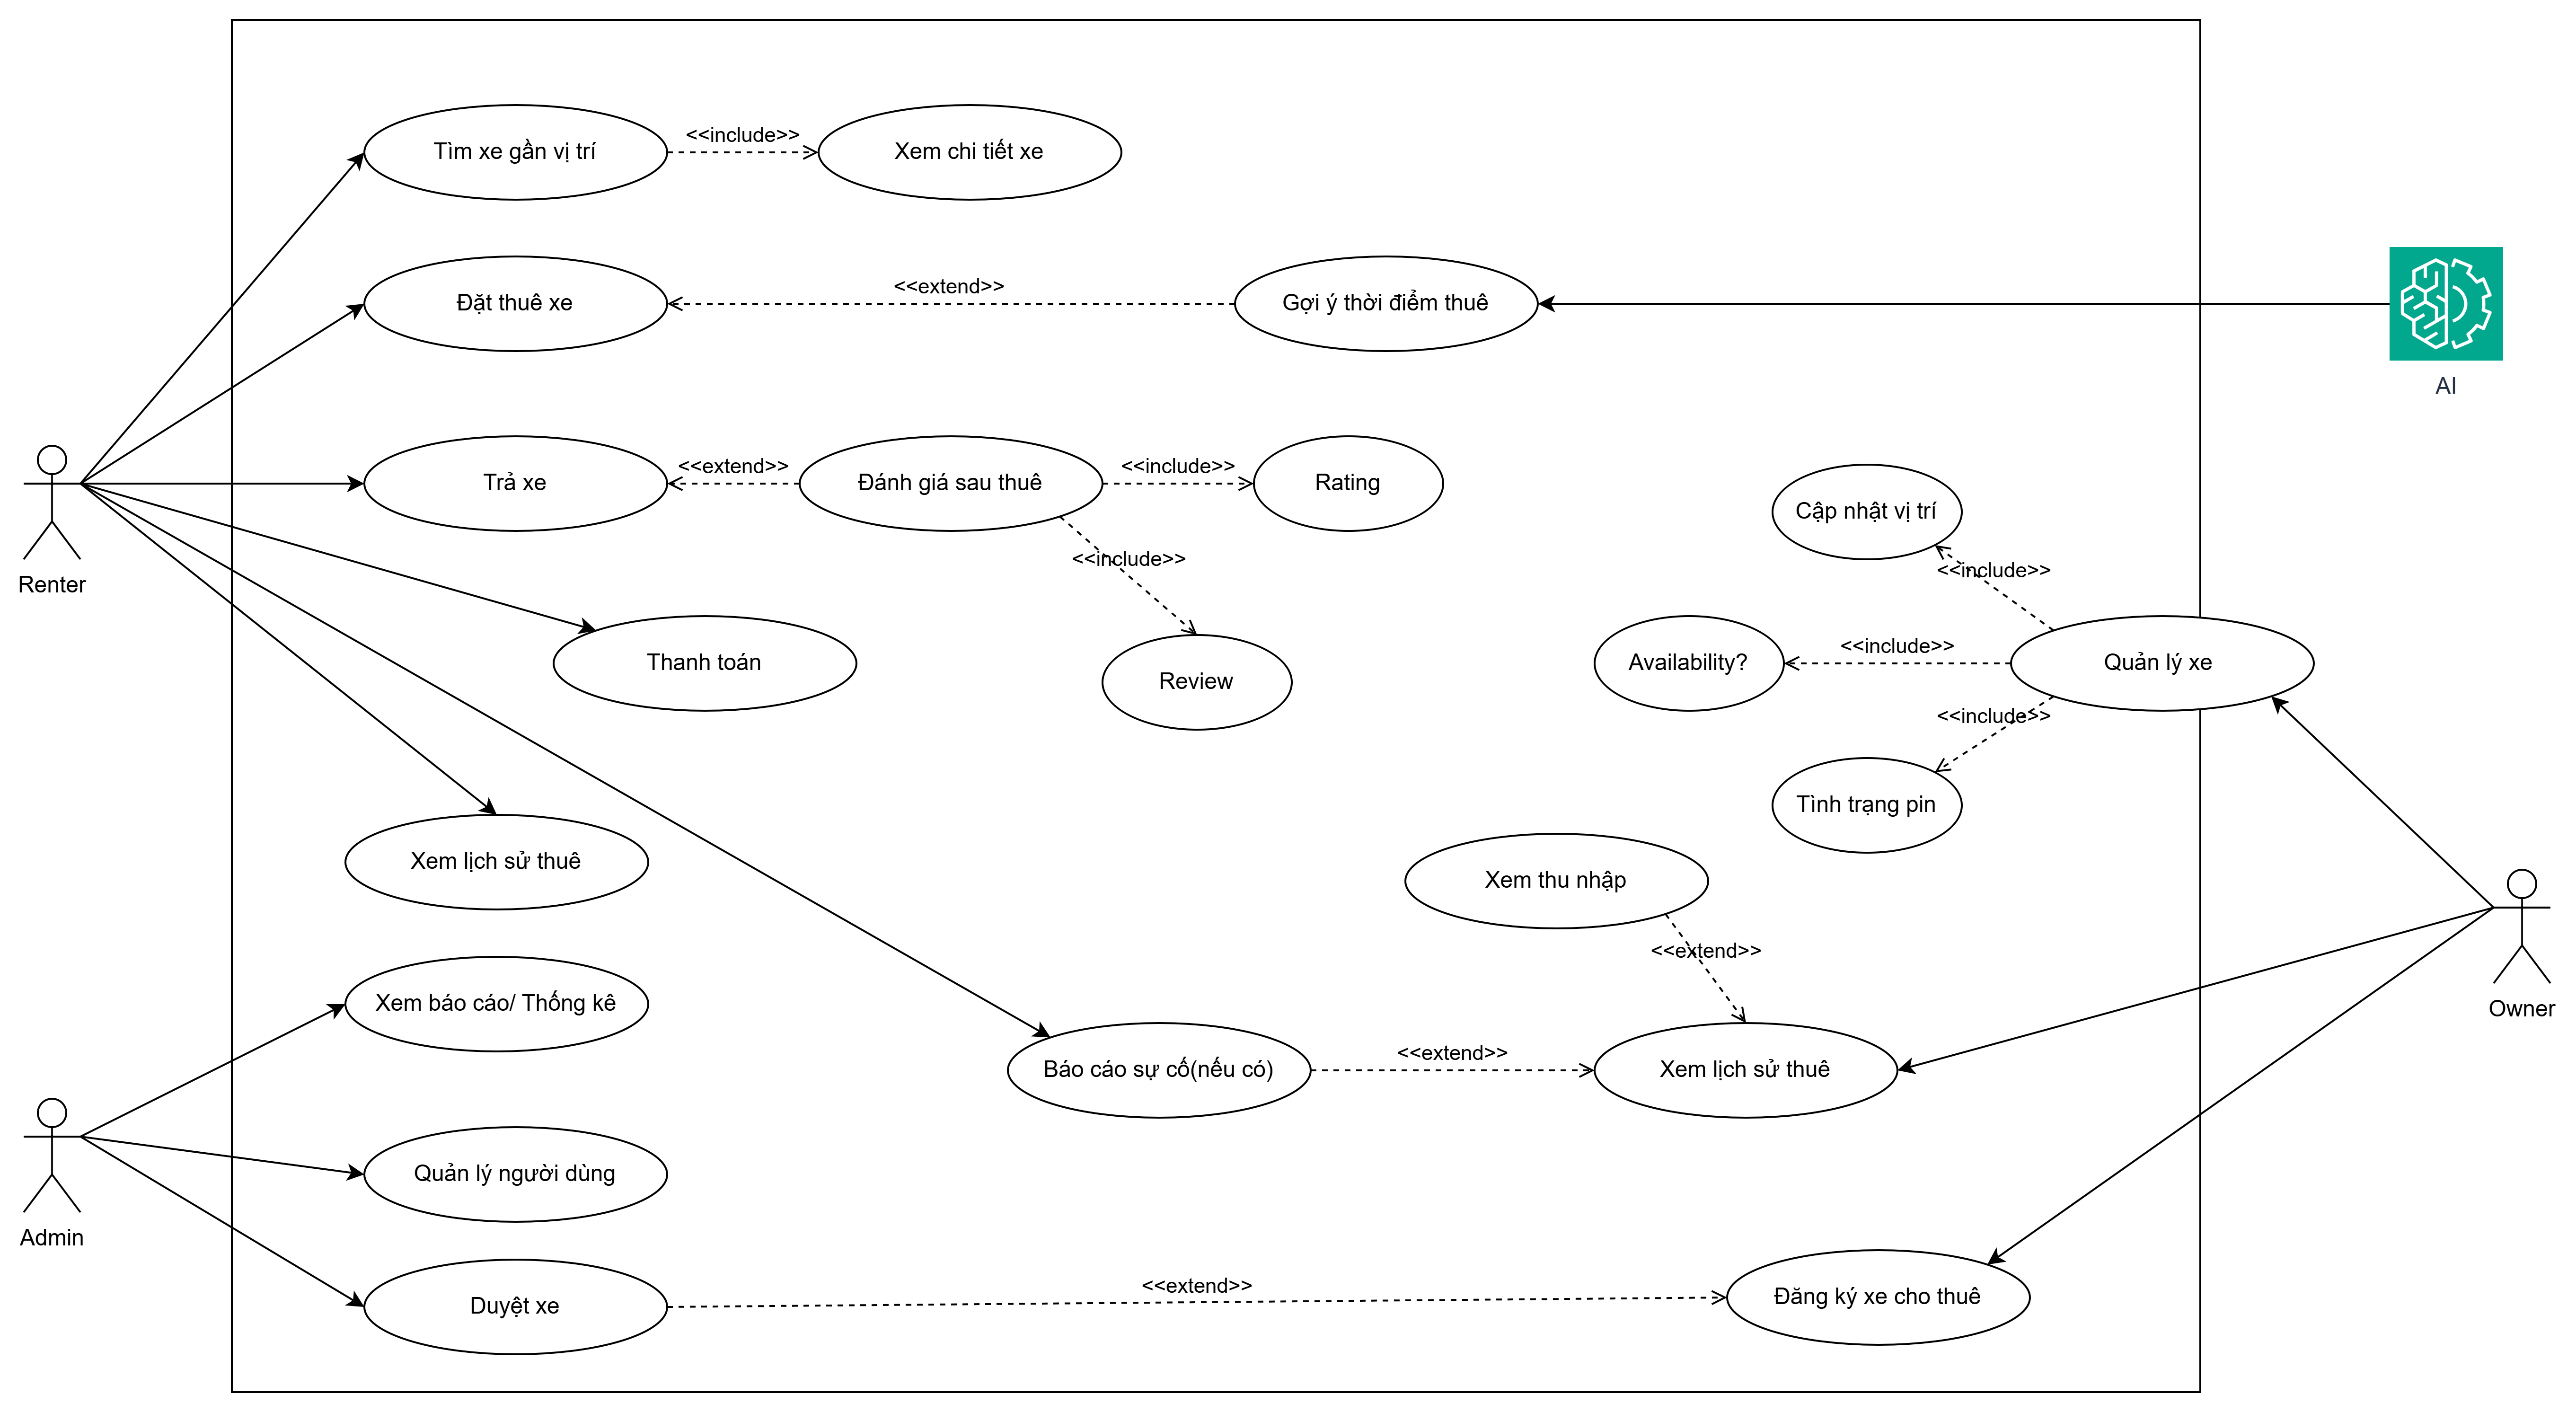
\includegraphics[width=1\textwidth]{Images/Usecase/system.png}
    \caption{Application Use Case Diagram}
\end{figure}

\begin{itemize}
    \item \textbf{UC-01:} Đăng ký / Đăng nhập
    \item \textbf{UC-13:} Đánh giá \& Xếp hạng người dùng (Trust Score System)
    \item \textbf{UC-14:} Gợi ý thời điểm thuê (Recommendation)
    \item \textbf{UC-15:} Xem lịch sử thuê / thu nhập (của Owner hoặc Renter)
    \item \textbf{UC-16:} Báo cáo sự cố (Renter/Owner)
    \item \textbf{UC-17:} Thông báo
    \item \textbf{Renter Use Case}
    \item \textbf{Owner Use Case}
    \item \textbf{Admin Use Case}
\end{itemize}

\vspace{0.5cm}
\subsubsection*{Renter Use Case}
\begin{itemize}
    \item \textbf{UC-02:} Tìm xe gần vị trí
    \item \textbf{UC-03:} Xem chi tiết xe
    \item \textbf{UC-04:} Đặt thuê xe
    \item \textbf{UC-05:} Trả xe
    \item \textbf{UC-06:} Thanh toán
    \item \textbf{UC-07:} Đánh giá sau thuê (Rating / Review)
\end{itemize}
\begin{figure}[H]
    \centering
    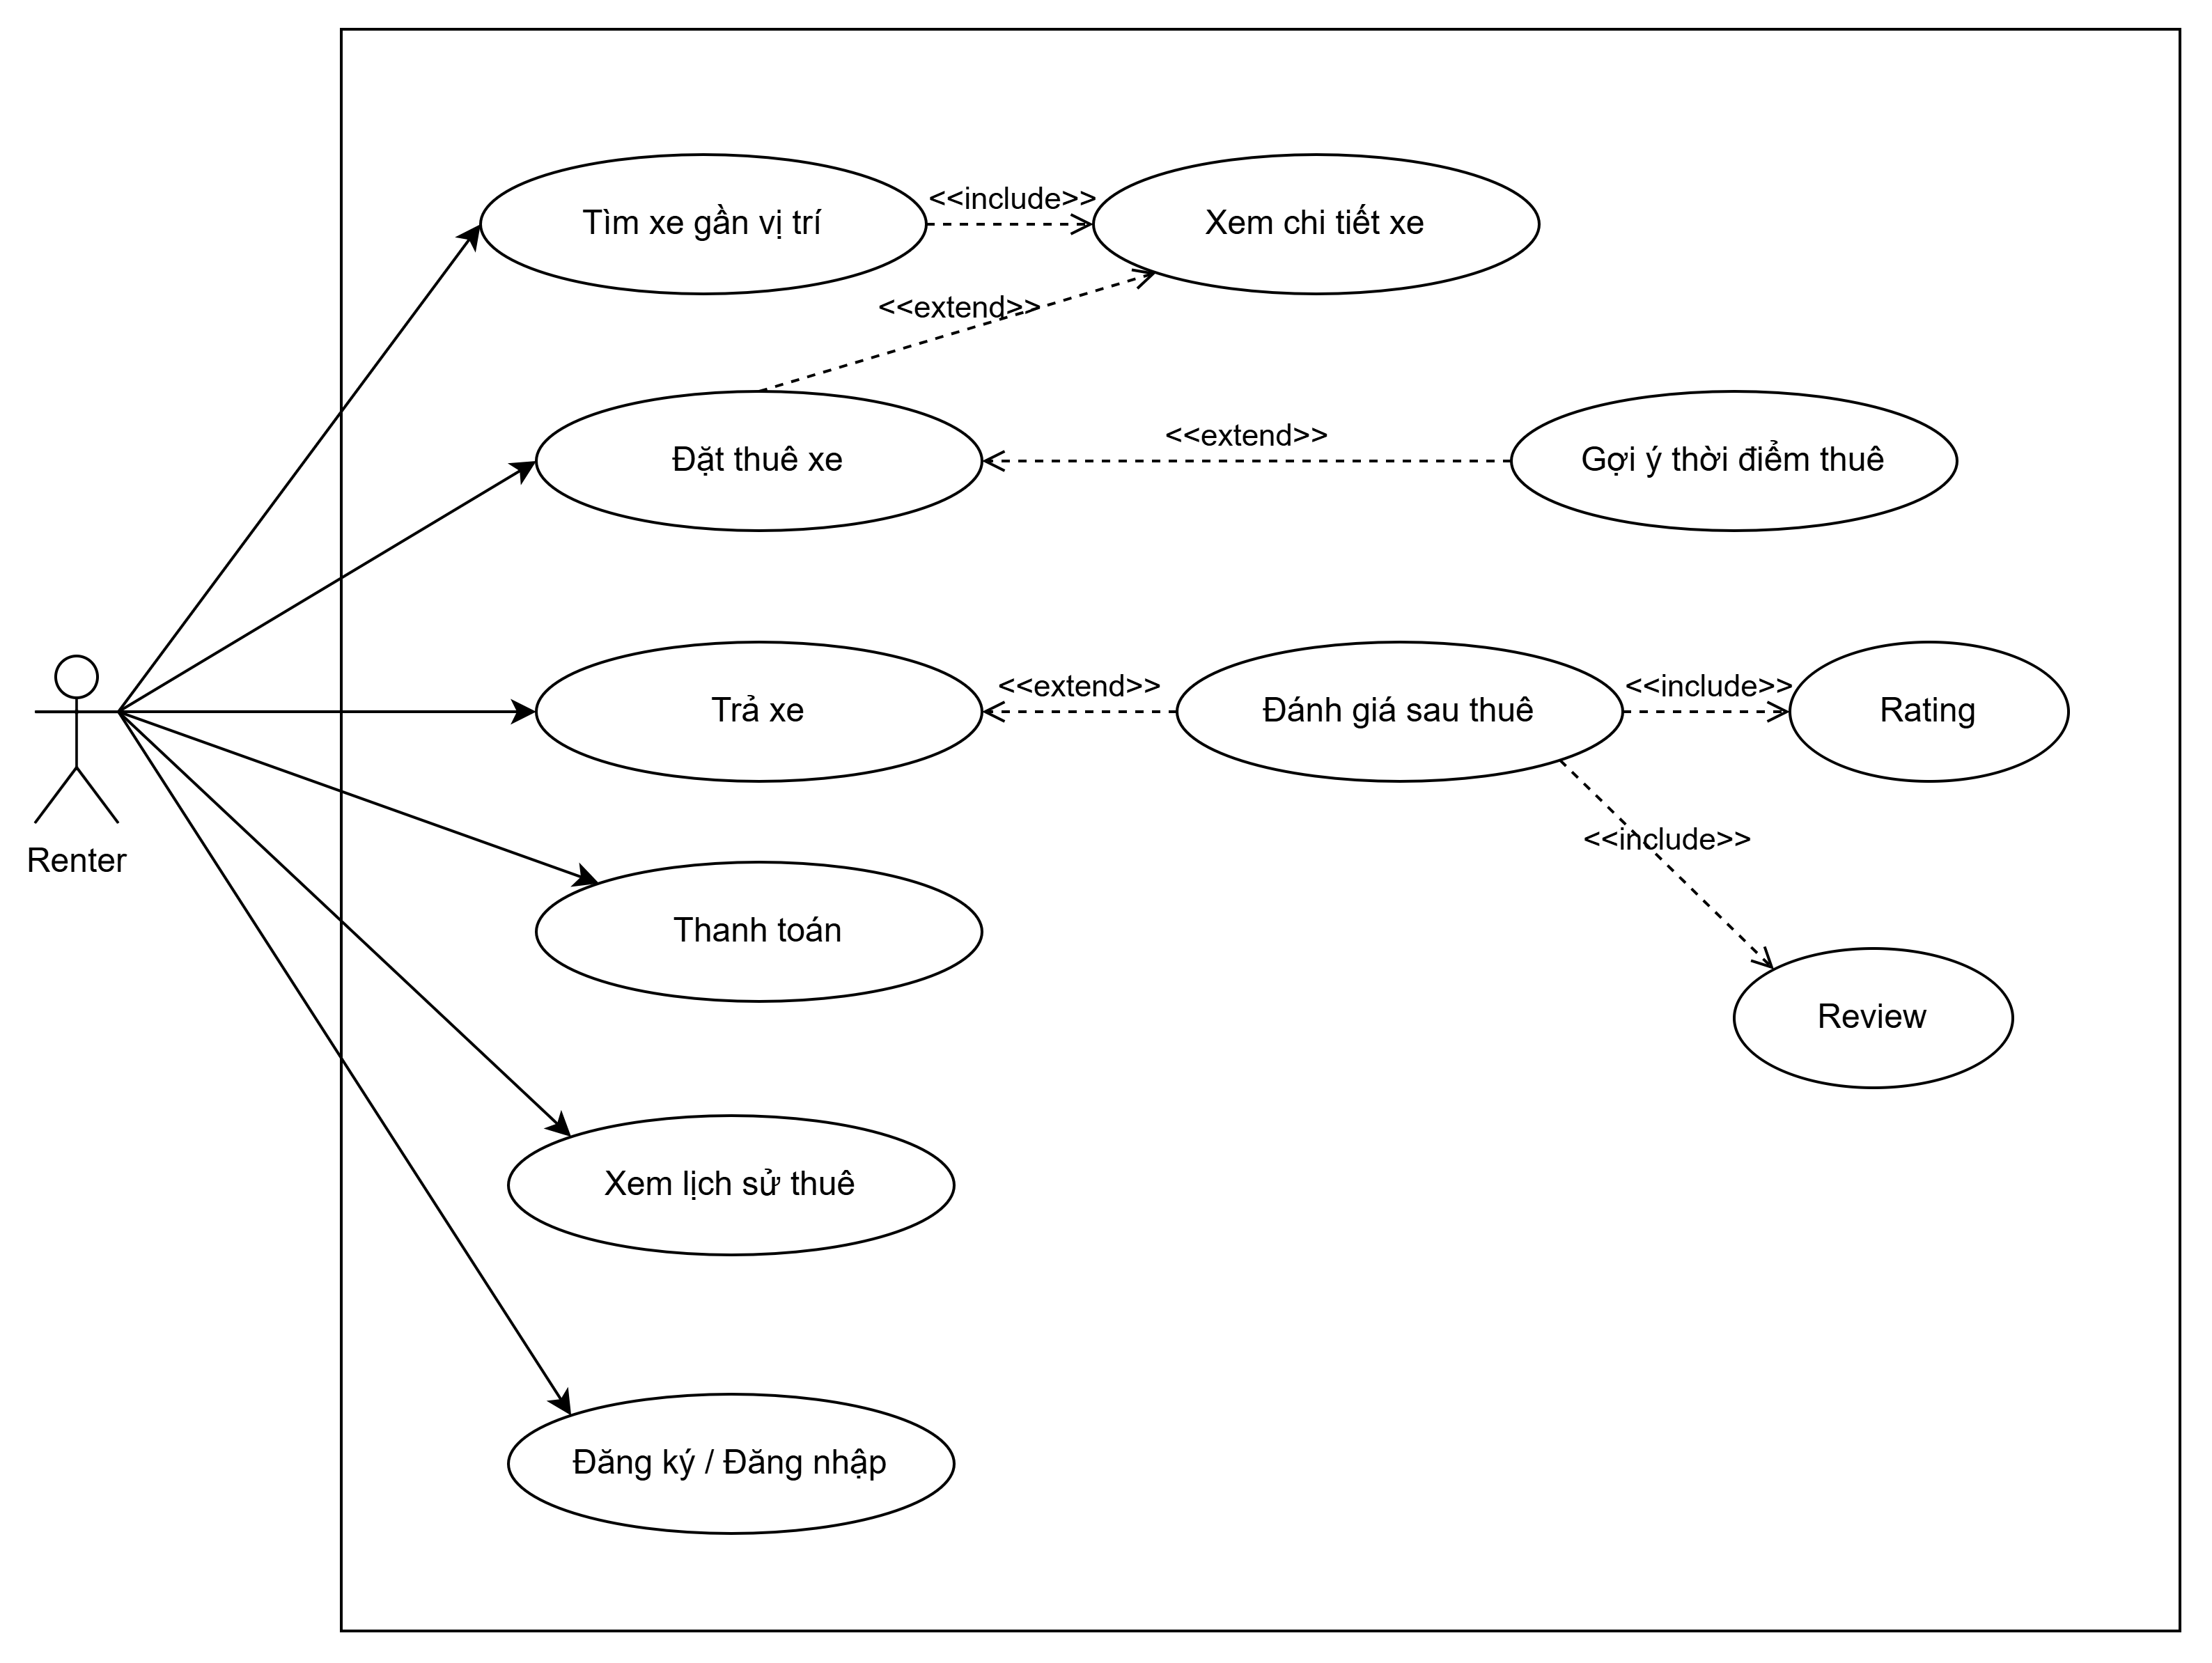
\includegraphics[width=0.85\textwidth]{Images/Usecase/renter.png}
    \caption{Renter Use Case Diagram}
\end{figure}

\subsubsection*{Owner Use Case}
\begin{itemize}
    \item \textbf{UC-08:} Đăng ký xe cho thuê (Owner)
    \item \textbf{UC-09:} Quản lý xe (Owner quản lý availability, cập nhật vị trí, pin)
\end{itemize}
\begin{figure}[H]
    \centering
    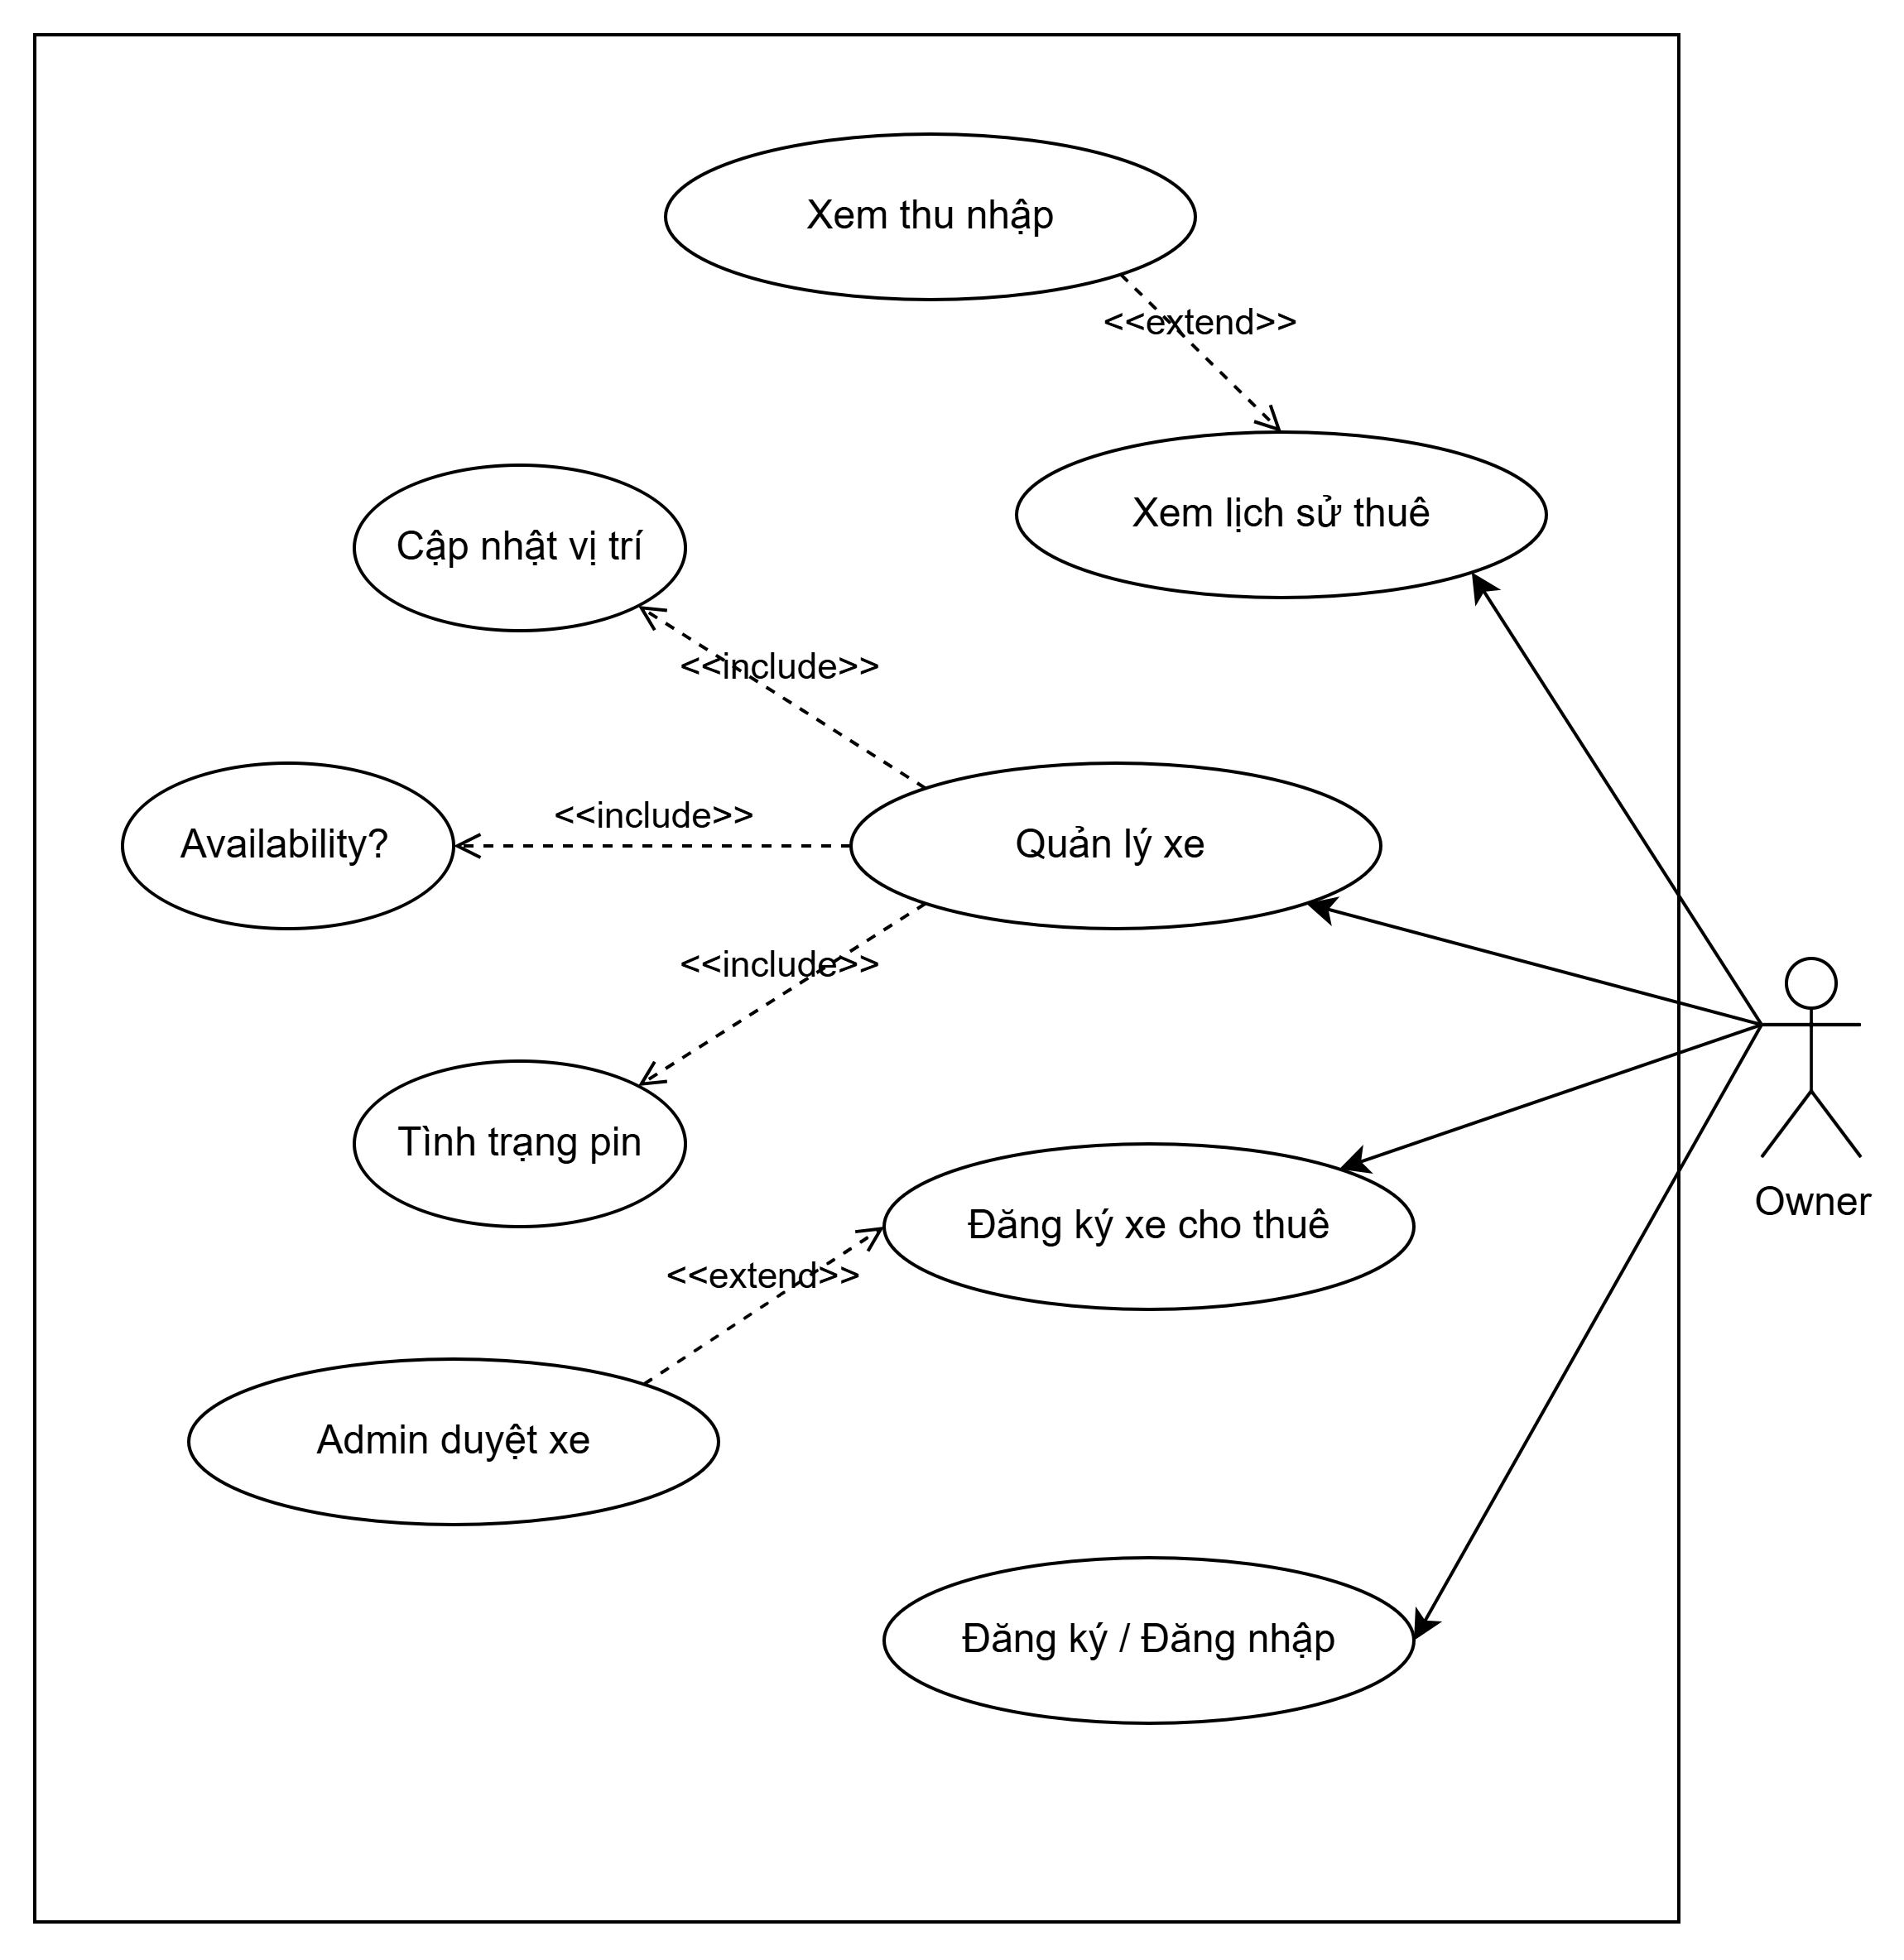
\includegraphics[width=0.65\textwidth]{Images/Usecase/owner.png}
    \caption{Owner Use Case Diagram}
\end{figure}

\subsubsection*{Admin Use Case}
\begin{figure}[H]
    \centering
    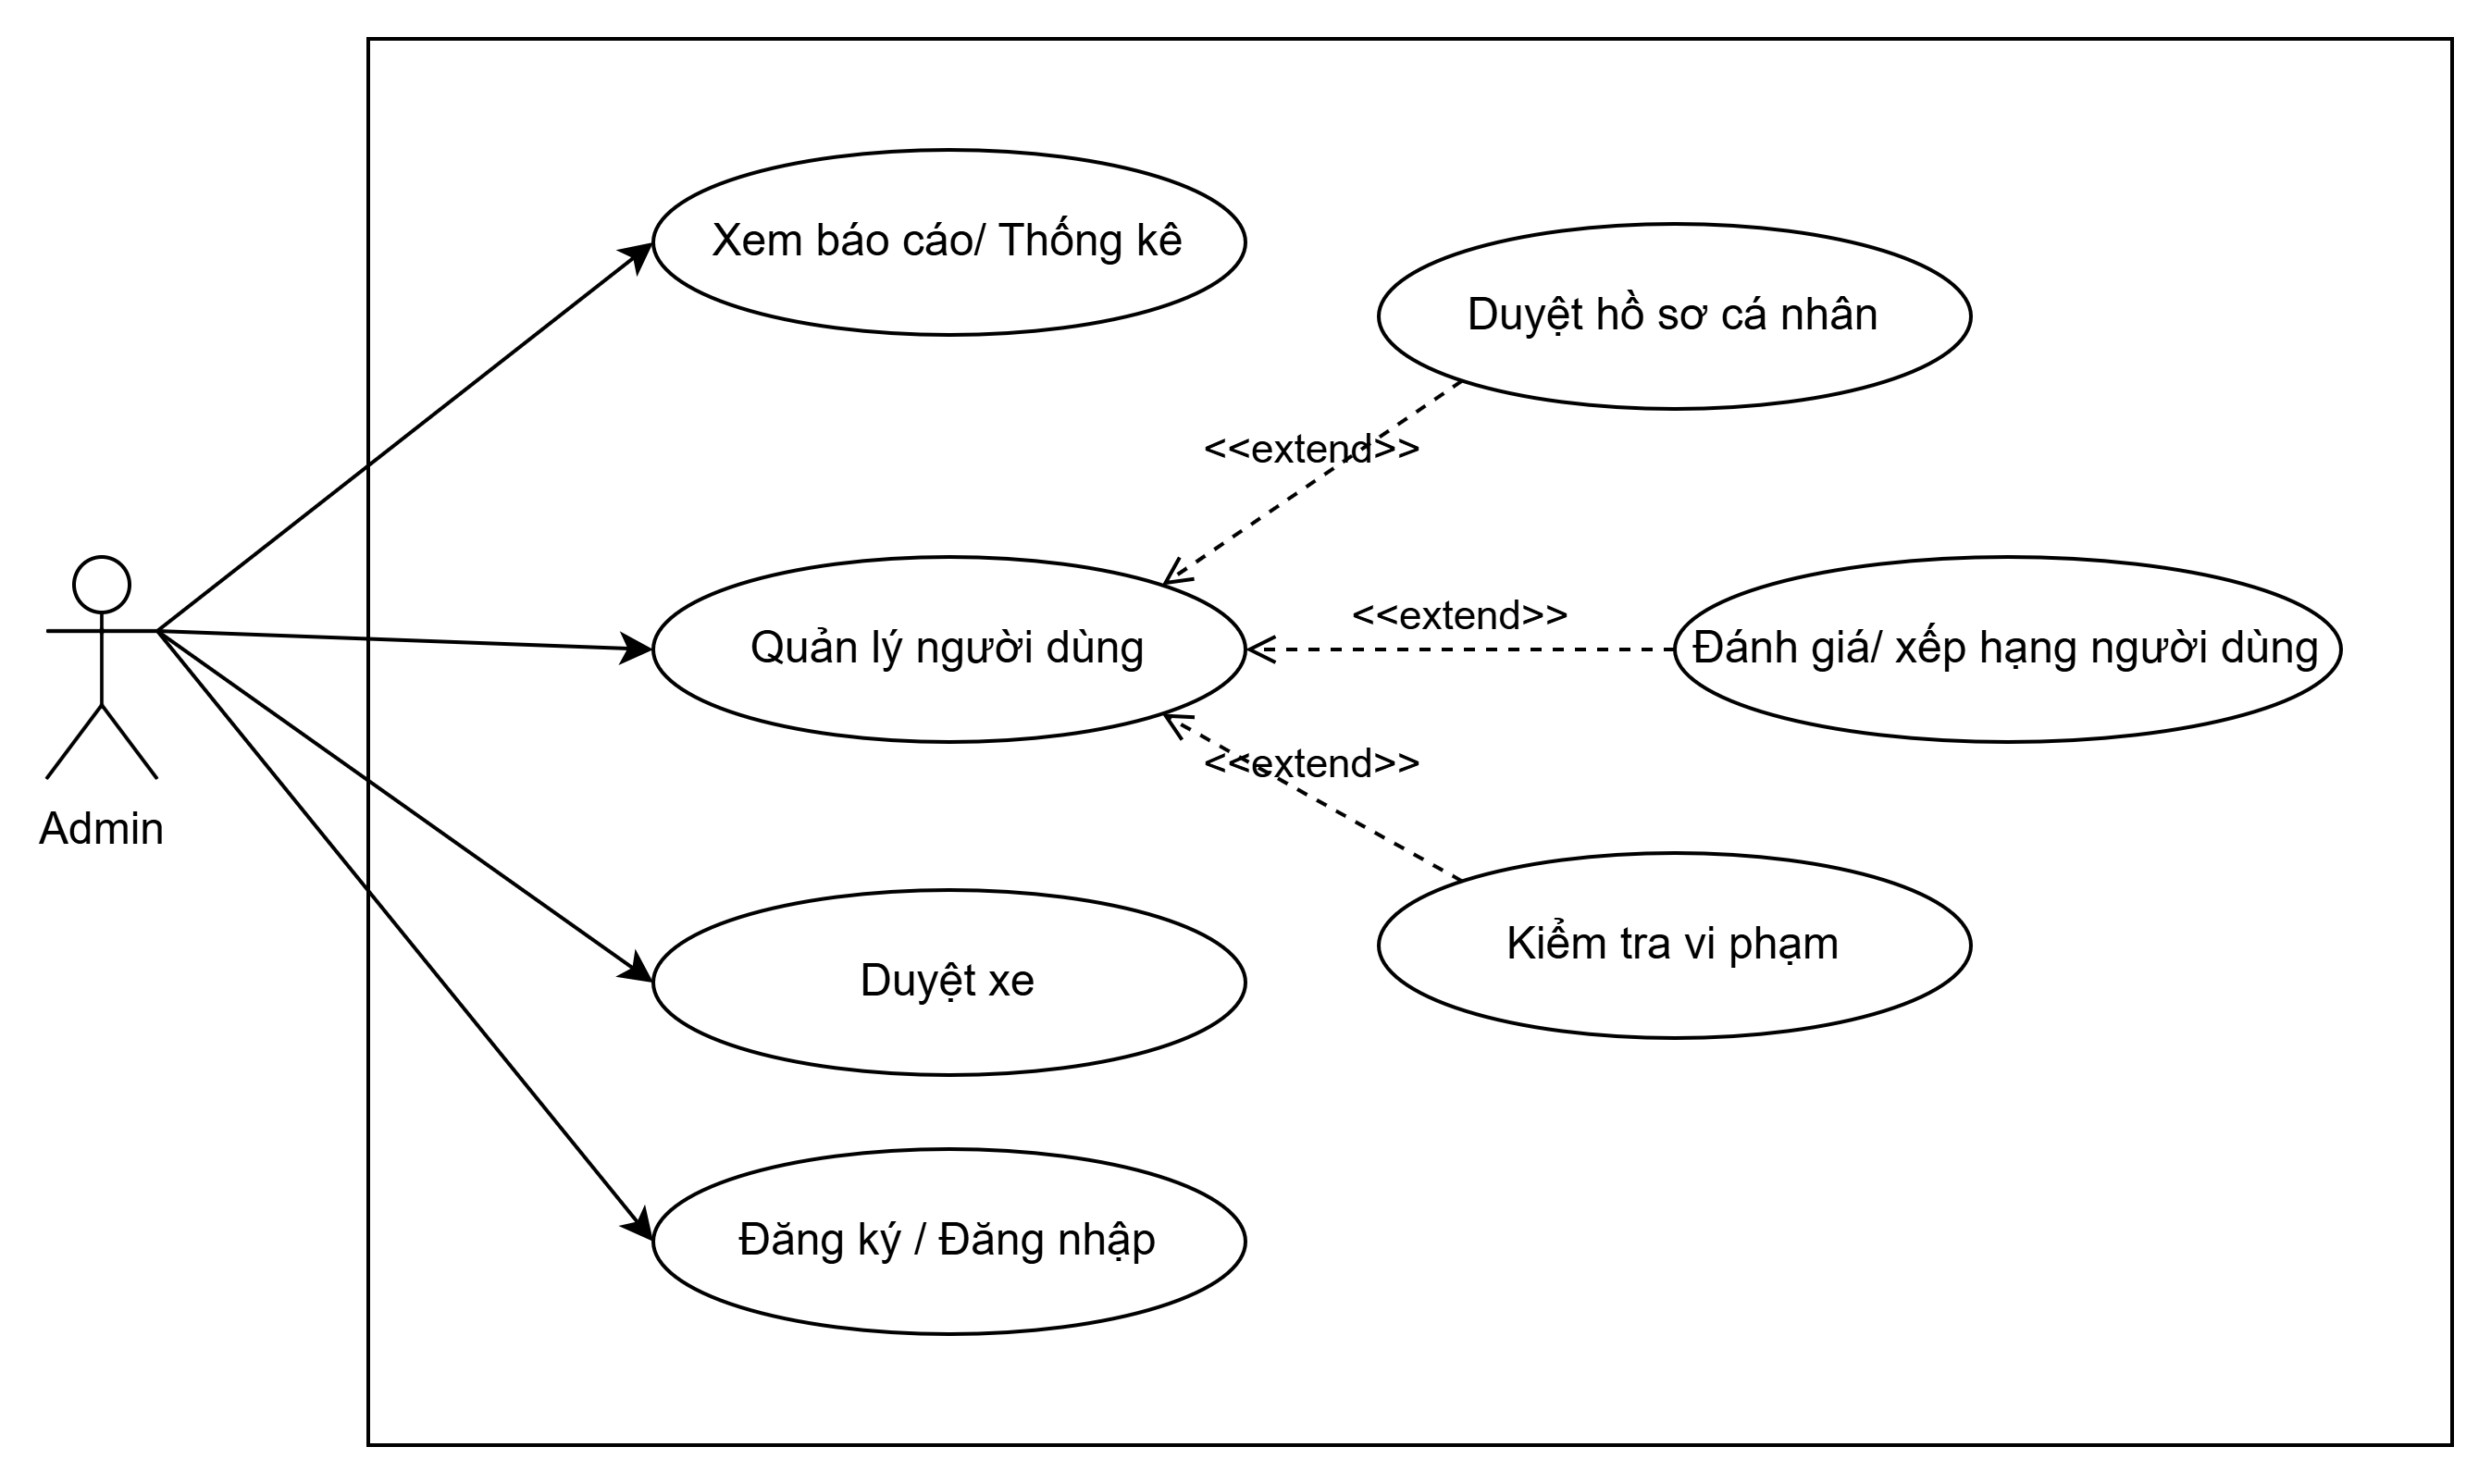
\includegraphics[width=0.65\textwidth]{Images/Usecase/admin.png}
    \caption{Admin Use Case Diagram}
\end{figure}

\begin{itemize}
    \item \textbf{UC-10:} Duyệt xe / Quản trị hệ thống (Admin)
    \item \textbf{UC-11:} Xem báo cáo / Thống kê (Admin)
    \item \textbf{UC-12:} Quản lý người dùng
\end{itemize}

\subsubsection{Use case description}

\subsubsection*{UC-01 –Đăng ký / Đăng nhập}

\begin{longtable}{|>{\raggedright\arraybackslash}p{4cm}|>{\raggedright\arraybackslash}p{11cm}|}
\hline
\textbf{Trường} & \textbf{Mô tả} \\
\hline
\endfirsthead

\hline
\textbf{Trường} & \textbf{Mô tả} \\
\hline
\endhead

\hline
\endfoot

Actor & Người dùng (Customer / Vehicle Owner / Admin) \\
\hline
Description & Người dùng đăng ký tài khoản mới hoặc đăng nhập vào hệ thống. \\
\hline
Trigger & Người dùng chọn "Đăng ký / Đăng nhập" trên giao diện. \\
\hline
Precondition & Ứng dụng hoạt động, có kết nối mạng. \\
\hline
Postcondition & Người dùng được xác thực và truy cập vào giao diện cá nhân. \\
\hline
Normal Flow & 1. Người dùng nhập email/số điện thoại và mật khẩu. \newline 2. Hệ thống kiểm tra thông tin. \newline 3. Nếu hợp lệ, đăng nhập thành công. \newline 4. Chuyển hướng tới màn hình chính. \\
\hline
Alt Flow & A1. Người dùng chọn "Quên mật khẩu" → Hệ thống gửi OTP khôi phục. \newline A2. Người dùng chọn "Đăng ký" → điền thông tin, gửi yêu cầu xác thực. \\
\hline
Exception Flow & E1. Sai mật khẩu quá 5 lần → tạm khóa tài khoản. \newline E2. Hệ thống lỗi kết nối → hiển thị thông báo "Không thể đăng nhập, vui lòng thử lại." \\
\hline
\end{longtable}

\subsubsection*{UC-02 – Tìm xe gần vị trí}

\begin{longtable}{|>{\raggedright\arraybackslash}p{4cm}|>{\raggedright\arraybackslash}p{11cm}|}
\hline
\textbf{Trường} & \textbf{Mô tả} \\
\hline
\endfirsthead

\hline
\textbf{Trường} & \textbf{Mô tả} \\
\hline
\endhead

\hline
\endfoot

\textbf{Tên Use Case} & Tìm xe gần vị trí \\
\hline
\textbf{Actor chính} & Người thuê xe (Renter) \\
\hline
\textbf{Mục tiêu} & Giúp người dùng tìm xe khả dụng trong khu vực xung quanh, dựa trên \textbf{vị trí hiện tại (GPS)} hoặc \textbf{vị trí nhập tay} để đặt trước. \\
\hline
\textbf{Trigger} & Người dùng nhấn ``Tìm xe gần tôi'' hoặc chọn ``Nhập vị trí khác''. \\
\hline
\textbf{Precondition} & Người dùng đã đăng nhập; có quyền truy cập bản đồ; GPS được bật hoặc người dùng nhập vị trí thủ công. \\
\hline
\textbf{Postcondition} & Danh sách xe khả dụng được hiển thị theo khu vực được chọn. \\
\hline
\textbf{Normal Flow} & 
1. Người dùng chọn ``Tìm xe gần tôi''. \newline
2. Hệ thống yêu cầu quyền truy cập vị trí GPS. \newline
3. Ứng dụng lấy vị trí hiện tại của người dùng. \newline
4. Backend truy vấn danh sách xe khả dụng trong bán kính. \newline
5. Hệ thống hiển thị các xe gần nhất cùng thông tin: khoảng cách, mức pin, giá thuê, đánh giá. \newline
6. Người dùng chọn một xe để xem chi tiết. \\
\hline
\textbf{Alt Flow} & 
1. Người dùng chọn ``Nhập vị trí khác''. \newline
2. Hệ thống hiển thị hộp tìm kiếm địa điểm. \newline
3. Người dùng nhập địa chỉ hoặc khu vực mong muốn. \newline
4. Hệ thống sử dụng Geocoding API để lấy tọa độ (lat, lng). \newline
5. Backend truy vấn danh sách xe khả dụng quanh vị trí đó. \newline
5.1. Nếu có xe khả dụng, hiển thị danh sách. \newline
5.2. Nếu không có xe, gợi ý mở rộng bán kính hoặc chọn thời gian khác.\\
\hline
\textbf{Exception Flow} & 
E1. Không có xe khả dụng → hiển thị thông báo ``Không có xe trong khu vực này.'' \newline
E2. GPS bị tắt và người dùng không nhập vị trí → yêu cầu bật định vị hoặc nhập vị trí thủ công. \newline
E3. Lỗi kết nối mạng → hiển thị thông báo ``Không thể tải dữ liệu. Vui lòng thử lại.'' \\
\hline
\textbf{Included Use Cases} & \texttt{UC-03 -- Xem chi tiết xe} \\
\hline
\textbf{Extended Use Cases} & \texttt{UC-04 -- Đặt thuê xe (Pre-booking)} \\
\hline
\textbf{Business Rules} &
- Vị trí nhập tay phải nằm trong khu vực hoạt động của hệ thống. \newline
- Với khoảng cách > 10km, hệ thống gợi ý chuyển sang khu vực gần hơn hoặc chế độ giao xe (nếu có). \newline
- Khi ``Đặt trước'', chỉ hiển thị xe có trạng thái \texttt{available} trong khung thời gian đã chọn. \\
\hline
\end{longtable}

\subsubsection*{UC-03 – Xem chi tiết xe}

\begin{longtable}{|>{\raggedright\arraybackslash}p{4cm}|>{\raggedright\arraybackslash}p{11cm}|}
\hline
\textbf{Trường} & \textbf{Mô tả} \\
\hline
\endfirsthead

\hline
\textbf{Trường} & \textbf{Mô tả} \\
\hline
\endhead

\hline
\endfoot

% Use Case ID & UC-03 \\
% \hline
Actor & Người thuê (Renter), Chủ xe (Owner) \\
\hline
Mục tiêu & Cho phép người dùng xem thông tin chi tiết của xe, bao gồm tình trạng pin, vị trí, giá thuê, đánh giá và thông tin chủ xe. \\
\hline
Trigger & Người dùng chọn một xe từ danh sách hiển thị (từ UC-02: "Tìm xe gần vị trí"). \\
\hline
Precondition & Xe tồn tại và đang ở trạng thái "có sẵn (available)". \\
\hline
Postcondition & Thông tin chi tiết hiển thị cho người dùng. \\
\hline
Normal Flow & 1. Người thuê chọn xe từ bản đồ hoặc danh sách. \newline 2. Server trả thông tin: hình ảnh, loại xe, tình trạng pin, vị trí hiện tại, giá, đánh giá trung bình, chủ xe. \newline 3. Ứng dụng hiển thị giao diện chi tiết xe. \newline 4. Người thuê có thể chọn "Đặt thuê xe" \\
\hline
Alternative Flow & A1. Người thuê thêm xe vào danh sách "Yêu thích" (wishlist). \newline A2. Người thuê chia sẻ đường dẫn xe cho người khác (social sharing). \\
\hline
Exception Flow & E1. Xe đã bị ẩn hoặc đang thuê → hiển thị thông báo "Xe không khả dụng". \newline E2. Lỗi tải dữ liệu → hiển thị "Không thể tải thông tin xe". \\
\hline
Included Use Cases & \texttt{Xem đánh giá (Review)} \\
\hline
Extended Use Cases & \texttt{Đặt thuê xe (UC-04)} \\
\hline
\end{longtable}

\subsubsection*{UC-04 – Đặt thuê xe}

\begin{longtable}{|>{\raggedright\arraybackslash}p{4cm}|>{\raggedright\arraybackslash}p{11cm}|}
\hline
\textbf{Trường} & \textbf{Mô tả} \\
\hline
\endfirsthead

\hline
\textbf{Trường} & \textbf{Mô tả} \\
\hline
\endhead

\hline
\endfoot

Actor & Người thuê xe \\
\hline
Description & Đặt trước xe để thuê trong khoảng thời gian mong muốn. \\
\hline
Trigger & Người dùng nhấn "Đặt thuê" trên chi tiết xe. \\
\hline
Precondition & Xe đang ở trạng thái "Available", người dùng đã đăng nhập. \\
\hline
Postcondition & Đơn đặt xe được ghi nhận và chờ xác nhận. \\
\hline
Normal Flow & 1. Người dùng chọn thời gian thuê. \newline 2. Hệ thống gợi ý thời điểm thuê tối ưu (AI). \newline 3. Người dùng xác nhận đặt thuê. \newline 4. Hệ thống tạo đơn và gửi thông báo cho chủ xe. \\
\hline
Alt Flow & A1. Người thuê thay đổi thời gian thuê → hệ thống cập nhật chi phí tương ứng. \newline A2. Chủ xe từ chối yêu cầu thuê. \\
\hline
Exception Flow & E1. Xe đã được người khác đặt trước → hiển thị thông báo lỗi. \newline E2. Lỗi thanh toán hoặc xác nhận mạng. \\
\hline
Extended Use Cases & \texttt{Gợi ý thời điểm thuê} \\
\hline
\end{longtable}

\subsubsection*{UC-05 – Trả xe}

\begin{longtable}{|>{\raggedright\arraybackslash}p{4cm}|>{\raggedright\arraybackslash}p{11cm}|}
\hline
\textbf{Trường} & \textbf{Mô tả} \\
\hline
\endfirsthead

\hline
\textbf{Trường} & \textbf{Mô tả} \\
\hline
\endhead

\hline
\endfoot

Actor & Người thuê xe \\
\hline
Description & Người thuê kết thúc hành trình và trả xe. \\
\hline
Trigger & Người thuê chọn "Trả xe" trên giao diện. \\
\hline
Precondition & Xe đang trong trạng thái thuê. \\
\hline
Postcondition & Xe được cập nhật trạng thái "Available". \\
\hline
Normal Flow & 1. Người thuê xác nhận trả xe. \newline 2. Hệ thống cập nhật vị trí trả xe và tính tổng chi phí. \newline 3. Thanh toán hoàn tất. \newline 4. Hiển thị màn hình đánh giá. \\
\hline
Alt Flow & A1. Người thuê trả xe sớm hơn dự kiến → hệ thống điều chỉnh chi phí. \\
\hline
Exception Flow & E1. Không thể xác định vị trí xe → yêu cầu nhập vị trí thủ công. \newline E2. Lỗi hệ thống thanh toán. \\
\hline
Extended Use Cases & \texttt{Đánh giá sau thuê} \\
\hline
\end{longtable}

\subsubsection*{UC-06 – Thanh toán}

\begin{longtable}{|>{\raggedright\arraybackslash}p{4cm}|>{\raggedright\arraybackslash}p{11cm}|}
\hline
\textbf{Trường} & \textbf{Mô tả} \\
\hline
\endfirsthead

\hline
\textbf{Trường} & \textbf{Mô tả} \\
\hline
\endhead

\hline
\endfoot

Actor & Người thuê xe \\
\hline
Description & Thực hiện thanh toán sau khi hoàn tất thuê xe hoặc đặt cọc trước khi thuê. \\
\hline
Trigger & Khi người dùng hoàn tất hành trình hoặc xác nhận đặt thuê. \\
\hline
Precondition & Người dùng đã chọn phương thức thanh toán (thẻ, ví điện tử, v.v.). \\
\hline
Postcondition & Giao dịch thanh toán thành công, lưu thông tin hóa đơn. \\
\hline
Normal Flow & 1. Hệ thống tính toán chi phí thuê (thời gian × giá). \newline 2. Hiển thị tổng tiền và yêu cầu xác nhận thanh toán. \newline 3. Người dùng xác nhận. \newline 4. Hệ thống kết nối cổng thanh toán (mock/payment gateway). \newline 5. Trạng thái cập nhật thành "Paid". \\
\hline
Alt Flow & A1. Người thuê chọn thanh toán bằng điểm thưởng hoặc ví điện tử nội bộ. \newline A2. Thanh toán tự động qua thẻ lưu sẵn. \\
\hline
Exception Flow & E1. Giao dịch thất bại → hoàn tác đặt xe. \newline E2. Cổng thanh toán không phản hồi → thông báo "Thử lại sau". \\
\hline
\end{longtable}

\subsubsection*{UC-07 – Đánh giá sau thuê}

\begin{longtable}{|>{\raggedright\arraybackslash}p{4cm}|>{\raggedright\arraybackslash}p{11cm}|}
\hline
\textbf{Trường} & \textbf{Mô tả} \\
\hline
\endfirsthead

\hline
\textbf{Trường} & \textbf{Mô tả} \\
\hline
\endhead

\hline
\endfoot

Actor & Người thuê xe \\
\hline
Description & Người dùng để lại đánh giá và chấm sao cho xe/chủ xe. \\
\hline
Trigger & Sau khi trả xe hoặc từ trang "Lịch sử thuê". \\
\hline
Precondition & Đã hoàn tất thuê xe. \\
\hline
Postcondition & Đánh giá được lưu trữ và cập nhật điểm trung bình. \\
\hline
Normal Flow & 1. Người dùng chọn số sao (1--5). \newline 2. Nhập nội dung nhận xét. \newline 3. Hệ thống lưu và cập nhật thông tin vào hồ sơ xe/chủ xe. \\
\hline
Alt Flow & A1. Người dùng chỉ đánh giá mà không viết bình luận. \\
\hline
Exception Flow & E1. Mạng lỗi, không gửi được đánh giá. \\
\hline
Included Use Cases & \texttt{Rating}, \texttt{Review} \\
\hline
\end{longtable}

\subsubsection*{UC-08 – Đăng ký xe cho thuê}

\begin{longtable}{|>{\raggedright\arraybackslash}p{4cm}|>{\raggedright\arraybackslash}p{11cm}|}
\hline
\textbf{Trường} & \textbf{Mô tả} \\
\hline
\endfirsthead

\hline
\textbf{Trường} & \textbf{Mô tả} \\
\hline
\endhead

\hline
\endfoot

Actor & Chủ xe (Owner) \\
\hline
Description & Cho phép chủ xe thêm xe điện của mình vào hệ thống để cho thuê. \\
\hline
Trigger & Chủ xe chọn "Đăng ký xe cho thuê" trong ứng dụng. \\
\hline
Precondition & Đã đăng nhập và xác thực danh tính. \\
\hline
Postcondition & Xe được thêm vào hệ thống với trạng thái "Chờ duyệt". \\
\hline
Normal Flow & 1. Chủ xe nhập thông tin xe (biển số, model, dung lượng pin, giá, vị trí). \newline 2. Hệ thống xác nhận dữ liệu hợp lệ. \newline 3. Tạo bản ghi xe mới trong DB với trạng thái "pending". \newline 4. Gửi thông báo cho admin để duyệt xe. \\
\hline
Alt Flow & A1. Chủ xe chọn lưu bản nháp để cập nhật sau. \newline A2. Chủ xe tải lại ảnh hoặc cập nhật thông tin trước khi gửi. \\
\hline
Exception Flow & E1. Trùng biển số với xe khác → báo lỗi. \newline E2. Ảnh không hợp lệ / sai định dạng. \newline E3. Lỗi kết nối tới server. \\
\hline
Extended Use Cases & \texttt{Duyệt xe} (Admin duyệt để xe có thể hoạt động) \\
\hline
\end{longtable}

\subsubsection*{UC-09 – Quản lý xe của chủ}

\begin{longtable}{|>{\raggedright\arraybackslash}p{4cm}|>{\raggedright\arraybackslash}p{11cm}|}
\hline
\textbf{Trường} & \textbf{Mô tả} \\
\hline
\endfirsthead

\hline
\textbf{Trường} & \textbf{Mô tả} \\
\hline
\endhead

\hline
\endfoot

Actor & Chủ xe \\
\hline
Description & Quản lý danh sách xe đã đăng ký, cập nhật thông tin hoặc tình trạng sẵn sàng cho thuê. \\
\hline
Trigger & Chủ xe mở mục "Quản lý xe". \\
\hline
Precondition & Chủ xe đã có ít nhất 1 xe đăng ký. \\
\hline
Postcondition & Thông tin xe được cập nhật, đồng bộ lên hệ thống. \\
\hline
Normal Flow & 1. Hệ thống hiển thị danh sách xe của chủ. \newline 2. Chủ xe chọn một xe → xem chi tiết. \newline 3. Có thể cập nhật giá, trạng thái pin, vị trí, khả dụng (availability). \newline 4. Hệ thống lưu và phản ánh thay đổi lên bản đồ. \\
\hline
Alt Flow & A1. Chủ xe tạm ẩn xe khỏi danh sách cho thuê. \newline A2. Chủ xe cập nhật vị trí tự động qua GPS. \\
\hline
Exception Flow & E1. Xe đang cho thuê không thể bị xóa hoặc ẩn. \newline E2. Cập nhật thất bại do mất kết nối. \\
\hline
Included Use Cases & \texttt{Cập nhật vị trí}, \texttt{Tình trạng pin}, \texttt{Availability} \\
\hline
\end{longtable}

\subsubsection*{UC-10 – Duyệt xe (Admin)}

\begin{longtable}{|>{\raggedright\arraybackslash}p{4cm}|>{\raggedright\arraybackslash}p{11cm}|}
\hline
\textbf{Trường} & \textbf{Mô tả} \\
\hline
\endfirsthead

\hline
\textbf{Trường} & \textbf{Mô tả} \\
\hline
\endhead

\hline
\endfoot

Actor & Quản trị viên \\
\hline
Description & Xem, kiểm duyệt và phê duyệt các xe được đăng ký bởi chủ xe. \\
\hline
Trigger & Admin đăng nhập vào bảng quản trị. \\
\hline
Precondition & Xe mới đăng ký có trạng thái "pending". \\
\hline
Postcondition & Xe được duyệt (status = "active") hoặc từ chối. \\
\hline
Normal Flow & 1. Admin mở danh sách xe chờ duyệt. \newline 2. Xem thông tin, hình ảnh, giấy tờ. \newline 3. Chọn "Phê duyệt" hoặc "Từ chối". \newline 4. Hệ thống cập nhật trạng thái và thông báo cho chủ xe. \\
\hline
Alt Flow & A1. Admin yêu cầu bổ sung giấy tờ trước khi duyệt. \\
\hline
Exception Flow & E1. Dữ liệu xe không hợp lệ hoặc lỗi kết nối DB. \\
\hline
\end{longtable}

\subsubsection*{UC-11 – Xem báo cáo / thống kê}

\begin{longtable}{|>{\raggedright\arraybackslash}p{4cm}|>{\raggedright\arraybackslash}p{11cm}|}
\hline
\textbf{Trường} & \textbf{Mô tả} \\
\hline
\endfirsthead

\hline
\textbf{Trường} & \textbf{Mô tả} \\
\hline
\endhead

\hline
\endfoot

Actor & Quản trị viên \\
\hline
Description & Xem các thống kê về số lượng thuê, doanh thu, hoạt động người dùng. \\
\hline
Trigger & Admin chọn "Thống kê / Báo cáo". \\
\hline
Precondition & Có dữ liệu hoạt động trên hệ thống. \\
\hline
Postcondition & Báo cáo hiển thị trên dashboard. \\
\hline
Normal Flow & 1. Admin chọn loại báo cáo (doanh thu, lượt thuê, hoạt động theo khu vực). \newline 2. Hệ thống tổng hợp dữ liệu từ DB. \newline 3. Hiển thị biểu đồ, bảng thống kê. \\
\hline
Alt Flow & A1. Admin chọn khoảng thời gian khác để xem. \newline A2. Xuất báo cáo ra file PDF. \\
\hline
Exception Flow & E1. Dữ liệu chưa được cập nhật kịp thời. \newline E2. Lỗi truy vấn SQL hoặc timeout. \\
\hline
\end{longtable}

\subsubsection*{UC-12 – Quản lý người dùng (Admin)}

\begin{longtable}{|>{\raggedright\arraybackslash}p{4cm}|>{\raggedright\arraybackslash}p{11cm}|}
\hline
\textbf{Trường} & \textbf{Mô tả} \\
\hline
\endfirsthead

\hline
\textbf{Trường} & \textbf{Mô tả} \\
\hline
\endhead

\hline
\endfoot

Actor & Quản trị viên \\
\hline
Description & Theo dõi, khóa, hoặc cấp quyền cho người dùng hệ thống. \\
\hline
Trigger & Admin truy cập mục "Quản lý người dùng". \\
\hline
Precondition & Admin đăng nhập thành công. \\
\hline
Postcondition & Người dùng bị cập nhật trạng thái hoặc quyền hạn. \\
\hline
Normal Flow & 1. Hệ thống hiển thị danh sách người dùng. \newline 2. Admin tìm kiếm theo tên/email. \newline 3. Admin có thể khóa, mở khóa, hoặc thay đổi quyền. \\
\hline
Alt Flow & A1. Admin gửi thông báo cảnh cáo tới người dùng vi phạm. \newline A2. Cấp quyền "Owner" cho người dùng mới. \\
\hline
Exception Flow & E1. Không có quyền đủ để sửa người dùng khác cấp cao hơn. \newline E2. Lỗi truy cập cơ sở dữ liệu. \\
\hline
\end{longtable}

\subsubsection*{UC-13 – Đánh giá \& Xếp hạng người dùng (Trust Score System)}

\begin{longtable}{|>{\raggedright\arraybackslash}p{4cm}|>{\raggedright\arraybackslash}p{11cm}|}
\hline
\textbf{Trường} & \textbf{Mô tả} \\
\hline
\endfirsthead

\hline
\textbf{Trường} & \textbf{Mô tả} \\
\hline
\endhead

\hline
\endfoot

% Use Case ID & UC-14 \\
% \hline
Use Case Name & Đánh giá \& Xếp hạng người dùng (Trust Score System) \\
\hline
Actor & Người thuê (Renter), Chủ xe (Owner), Hệ thống AI/Backend \\
\hline
Description & Sau khi hoàn tất giao dịch, cả hai bên (người thuê và chủ xe) có thể đánh giá lẫn nhau. Hệ thống tổng hợp các đánh giá để xây dựng \textbf{chỉ số uy tín (Trust Score)} của mỗi người dùng. \\
\hline
Trigger & Kết thúc giao dịch thuê xe (hoặc định kỳ hệ thống cập nhật lại Trust Score). \\
\hline
Precondition & Giao dịch đã hoàn tất (status = "completed"). \\
\hline
Postcondition & Điểm Trust Score và đánh giá được cập nhật trong hồ sơ người dùng. \\
\hline
Normal Flow & 1. Sau khi hoàn tất chuyến thuê, hệ thống gửi yêu cầu đánh giá cho cả hai bên. \newline 2. Người thuê chấm sao và để lại nhận xét về chủ xe (thái độ, tình trạng xe, đúng giờ). \newline 3. Chủ xe chấm sao người thuê (cách sử dụng xe, đúng hẹn, hoàn trả đầy đủ). \newline 4. Hệ thống lưu cả hai đánh giá, cập nhật \textbf{Trust Score}: \newline Trust Score = average of (rating, dispute rate, activity, on-time return rate, verification level). \newline 5. Điểm Trust Score hiển thị công khai trên hồ sơ người dùng. \\
\hline
Alt Flow & A1. Một bên bỏ qua đánh giá → hệ thống gửi nhắc sau 24h. \newline A2. Người dùng báo cáo đánh giá sai lệch → admin can thiệp. \\
\hline
Exception Flow & E1. Mạng lỗi khi gửi đánh giá. \newline E2. Hệ thống AI không tính được Trust Score do thiếu dữ liệu. \\
\hline
Included Use Cases & \texttt{Rating}, \texttt{Review} \\
\hline
Extended Use Cases & \texttt{Phân tích uy tín bằng AI} (tùy chọn mở rộng sau này) \\
\hline
\end{longtable}

\subsubsection*{Mô hình dữ liệu Trust Score (gợi ý)}

\begin{longtable}{|>{\raggedright\arraybackslash}p{5cm}|>{\raggedright\arraybackslash}p{6cm}|>{\raggedright\arraybackslash}p{3cm}|}
\hline
\textbf{Thuộc tính} & \textbf{Nguồn dữ liệu} & \textbf{Trọng số} \\
\hline
\endfirsthead

\hline
\textbf{Thuộc tính} & \textbf{Nguồn dữ liệu} & \textbf{Trọng số} \\
\hline
\endhead

\hline
\endfoot

Điểm trung bình đánh giá & Review của các counterparties & 0.4 \\
\hline
Tỷ lệ hoàn trả đúng giờ & Rental History & 0.2 \\
\hline
Tỷ lệ tranh chấp (dispute) & Admin report & -0.2 \\
\hline
Xác thực tài khoản (KYC) & Verification API & 0.1 \\
\hline
Tần suất hoạt động / số giao dịch hoàn tất & Transaction logs & 0.1 \\
\hline
\end{longtable}

\subsubsection*{UC-15 – Xem lịch sử thuê / thu nhập}

\begin{longtable}{|>{\raggedright\arraybackslash}p{4cm}|>{\raggedright\arraybackslash}p{11cm}|}
\hline
\textbf{Trường} & \textbf{Mô tả} \\
\hline
\endfirsthead

\hline
\textbf{Trường} & \textbf{Mô tả} \\
\hline
\endhead

\hline
\endfoot

Actor & Người thuê / Chủ xe \\
\hline
Description & Xem danh sách các giao dịch thuê xe (đã, đang, hoặc sắp tới). Chủ xe có thể xem thu nhập. \\
\hline
Trigger & Người dùng chọn "Lịch sử thuê" hoặc "Doanh thu". \\
\hline
Precondition & Đã đăng nhập. \\
\hline
Postcondition & Hiển thị danh sách lịch sử có thể lọc theo thời gian. \\
\hline
Normal Flow & 1. Gửi yêu cầu tới server \texttt{/rentals?userId=}. \newline 2. Hệ thống trả về danh sách và tổng thu nhập (đối với chủ xe). \newline 3. Người dùng có thể xem chi tiết từng giao dịch. \\
\hline
Alt Flow & A1. Lọc theo ngày, khu vực, loại xe. \newline A2. Xuất dữ liệu thành file CSV/PDF. \\
\hline
Exception Flow & E1. Không có dữ liệu phù hợp → hiển thị thông báo. \newline E2. Lỗi DB hoặc timeout. \\
\hline
Extended Use Cases & \texttt{Xem thu nhập} (dành riêng cho chủ xe) \\
\hline
\end{longtable}

\subsubsection*{UC-14 – Gợi ý thời điểm thuê (AI Module)}

\begin{longtable}{|>{\raggedright\arraybackslash}p{4cm}|>{\raggedright\arraybackslash}p{11cm}|}
\hline
\textbf{Trường} & \textbf{Mô tả} \\
\hline
\endfirsthead

\hline
\textbf{Trường} & \textbf{Mô tả} \\
\hline
\endhead

\hline
\endfoot

Actor & Người thuê xe, Hệ thống AI \\
\hline
Description & Hệ thống gợi ý thời gian thuê phù hợp dựa trên dữ liệu lịch sử và hành vi người dùng. \\
\hline
Trigger & Người dùng chọn "Gợi ý thời điểm thuê". \\
\hline
Precondition & Hệ thống có dữ liệu lịch sử giao dịch. \\
\hline
Postcondition & Gợi ý hiển thị trên giao diện. \\
\hline
Normal Flow & 1. Người dùng yêu cầu gợi ý. \newline 2. Backend gửi dữ liệu lịch sử cho mô hình ML. \newline 3. ML xử lý và trả về khung giờ gợi ý cùng độ tin cậy (confidence). \newline 4. Hệ thống hiển thị cho người dùng. \\
\hline
Alt Flow & A1. Nếu chưa có dữ liệu lịch sử → hiển thị khuyến nghị mặc định (rule-based). \\
\hline
Exception Flow & E1. AI service tạm ngưng → hiển thị lỗi "Dịch vụ không khả dụng". \\
\hline
\end{longtable}

\subsubsection*{UC-16 – Báo cáo sự cố (Incident Report)}

\begin{longtable}{|>{\raggedright\arraybackslash}p{4cm}|>{\raggedright\arraybackslash}p{11cm}|}
\hline
\textbf{Trường} & \textbf{Mô tả} \\
\hline
\endfirsthead

\hline
\textbf{Trường} & \textbf{Mô tả} \\
\hline
\endhead

\hline
\endfoot

% Use Case ID & UC-16 \\
% \hline
Actor & Người thuê (Renter), Chủ xe (Owner), Quản trị viên (Admin) \\
\hline
Mục tiêu & Cho phép người dùng báo cáo sự cố trong quá trình thuê xe hoặc phát hiện vấn đề với phương tiện. \\
\hline
Trigger & Người dùng chọn "Báo cáo sự cố" trong giao diện "Theo dõi chuyến đi" hoặc sau khi hoàn tất thuê. \\
\hline
Precondition & Có chuyến thuê đang hoạt động hoặc vừa hoàn tất. \\
\hline
Postcondition & Báo cáo được lưu vào hệ thống và chờ Admin xử lý. \\
\hline
Normal Flow & 1. Người thuê mở mục "Báo cáo sự cố". \newline 2. Chọn loại sự cố (xe không hoạt động, tai nạn, hư pin, mất xe, v.v.). \newline 3. Nhập mô tả chi tiết, kèm ảnh hoặc video. \newline 4. Hệ thống gửi dữ liệu đến server. \newline 5. Admin nhận thông báo và phản hồi qua trung tâm quản trị để xử lí. \\
\hline
Alternative Flow & A1. Chủ xe báo cáo sự cố do người thuê gây ra (ví dụ: trả xe không đúng vị trí, hư hỏng xe). \newline A2. Người thuê gửi thêm bằng chứng bổ sung sau khi tạo báo cáo. \\
\hline
Exception Flow & E1. Không tải được ảnh hoặc lỗi mạng → lưu tạm cục bộ, gửi lại khi có kết nối. \newline E2. Admin chưa phản hồi trong thời hạn → hệ thống gửi nhắc tự động. \\
\hline
Included Use Cases & \texttt{Thông báo (Notification)} \\
\hline
Extended Use Cases & \texttt{Xem lịch sử thuê (UC-15)} \\
\hline
\end{longtable}

\subsubsection*{UC-17 – Notification System}

\begin{longtable}{|>{\raggedright\arraybackslash}p{4cm}|>{\raggedright\arraybackslash}p{11cm}|}
\hline
\textbf{Trường} & \textbf{Mô tả} \\
\hline
\endfirsthead

\hline
\textbf{Trường} & \textbf{Mô tả} \\
\hline
\endhead

\hline
\endfoot

% Use Case ID & UC-17 \\
% \hline
Actor & Người thuê (Renter), Chủ xe (Owner), Quản trị viên (Admin), Hệ thống Notification Service \\
\hline
Mục tiêu & Gửi và hiển thị thông báo (real-time hoặc offline) khi có sự kiện liên quan trong hệ thống. \\
\hline
Trigger & Một sự kiện xảy ra trong hệ thống (ví dụ: thuê xe, trả xe, phê duyệt xe, đánh giá, báo cáo sự cố). \\
\hline
Precondition & Người dùng có tài khoản hợp lệ và đăng nhập vào hệ thống. \\
\hline
Postcondition & Thông báo được gửi đến đúng đối tượng và lưu lại trong lịch sử thông báo. \\
\hline
Normal Flow & 1. Một hành động hoặc sự kiện diễn ra, ví dụ: \newline - Người thuê gửi yêu cầu thuê xe (UC-04). \newline - Admin duyệt xe (UC-10). \newline - Người thuê đánh giá chủ xe (UC-07). \newline - Có báo cáo sự cố (UC-16). \newline 2. Backend tạo event. \newline 3. Notification Service nhận event từ hệ thống chính qua message queue (hoặc event bus). \newline 4. Tùy theo loại sự kiện, hệ thống xác định danh sách người nhận: \newline - \textbf{Renter}: thông báo xác nhận thuê / phản hồi từ Owner. \newline - \textbf{Owner}: thông báo khi có người muốn thuê / khi xe được trả. \newline - \textbf{Admin}: thông báo có sự cố hoặc cần duyệt xe. \newline 5. Gửi thông báo: \newline - \textbf{Real-time (push)}: thông qua Firebase Cloud Messaging hoặc WebSocket. \newline - \textbf{Offline (inbox)}: lưu trong bảng \texttt{notifications} để xem lại sau. \newline 6. Người dùng nhận thông báo trên ứng dụng (popup, icon badge, hoặc email). \\
\hline
Alternative Flow & A1. Người dùng tắt thông báo đẩy → Hệ thống chỉ lưu thông báo trong hộp thư (inbox), không push. \newline A2. Người dùng đã đọc thông báo → Trạng thái thông báo được cập nhật thành \texttt{read = true}. \newline A3. Người dùng xóa thông báo → Thông báo được ẩn khỏi giao diện nhưng vẫn lưu lịch sử trong DB. \\
\hline
Exception Flow & E1. Firebase / WebSocket mất kết nối → Thông báo sẽ được gửi lại khi người dùng online hoặc gửi email dự phòng. \newline E2. Event payload không hợp lệ → Notification Service ghi log lỗi và bỏ qua sự kiện. \newline E3. Người nhận không tồn tại hoặc đã bị khóa → Bỏ qua hoặc gửi thông báo tới Admin để kiểm tra. \\
\hline
% Included Use Cases & \\
% \hline
% Extended Use Cases & \\
% \hline
\end{longtable}

\subsection{Mô hình hoá quy trình nghiệp vụ}

% ---------------------- RENT PROCESS ----------------------
\subsubsection{Quy trình thuê xe (UC-02, UC-03, UC-04)}
\label{subsec:rent-activity}
\small\textit{(Hình \ref{fig:rent-activity})}
\subsubsection*{Mục tiêu:}
Cho phép người dùng tìm kiếm, xem thông tin và đặt thuê xe máy điện trong khu vực mong muốn thông qua ứng dụng.
\subsubsection*{Actor chính: Người thuê (Renter)}
\subsubsection*{Các bước chính:}
1. Người thuê đăng nhập và chọn chức năng “Tìm xe gần tôi” hoặc nhập vị trí thủ công.\newline
2. Hệ thống xác định vị trí, truy vấn và hiển thị danh sách xe khả dụng.\newline
3. Người thuê chọn xe để xem thông tin chi tiết (giá, pin, vị trí, chủ xe, đánh giá).\newline
4. Người thuê chọn “Đặt thuê”, nhập thời gian và xác nhận.\newline
5. Hệ thống gợi ý thời điểm thuê tối ưu (AI), kiểm tra tình trạng xe, tạo đơn thuê và gửi thông báo đến chủ xe.\newline
6. Người thuê nhận xác nhận thành công, hoàn tất quá trình thuê nếu chủ xe xác nhận cho thuê.
\subsubsection*{Luồng thay thế:}
Người dùng có thể nhập vị trí thủ công khi không bật GPS. Nếu không có xe khả dụng, hệ thống gợi ý mở rộng phạm vi hoặc thời gian khác.

% ---------------------- RETURN PROCESS ----------------------
\subsubsection{Quy trình trả xe (UC-05, UC-06, UC-07)}
\label{subsec:return-activity}
\small\textit{(Hình \ref{fig:return-activity})}
\subsubsection*{Mục tiêu:}
Cho phép người thuê kết thúc hành trình, trả xe và thực hiện thanh toán, đồng thời gửi đánh giá cho chủ xe hoặc phương tiện sau khi hoàn tất chuyến đi.
\subsubsection*{Actor chính: Người thuê (Renter)}
\subsubsection*{Các bước chính:}
1. Người thuê chọn chức năng “Trả xe” trong ứng dụng. \newline
2. Hệ thống xác nhận vị trí hiện tại của xe hoặc yêu cầu nhập thủ công nếu không định vị được. \newline
3. Hệ thống tính toán chi phí thuê thực tế dựa trên thời gian và quãng đường. \newline
4. Người thuê xác nhận thanh toán. \newline
5. Sau khi thanh toán thành công, hệ thống cập nhật trạng thái xe thành “Available”. \newline
6. Ứng dụng hiển thị màn hình đánh giá xe và chủ xe. \newline
7. Người thuê gửi đánh giá (số sao, nội dung) để hoàn tất quy trình.
\subsubsection*{Luồng thay thế:}
- Nếu người thuê trả xe sớm hơn thời gian dự kiến, hệ thống tự động điều chỉnh chi phí. \newline
- Nếu GPS không xác định được vị trí, hệ thống yêu cầu người dùng nhập vị trí trả xe thủ công.

\begin{figure}[H]
    \centering
    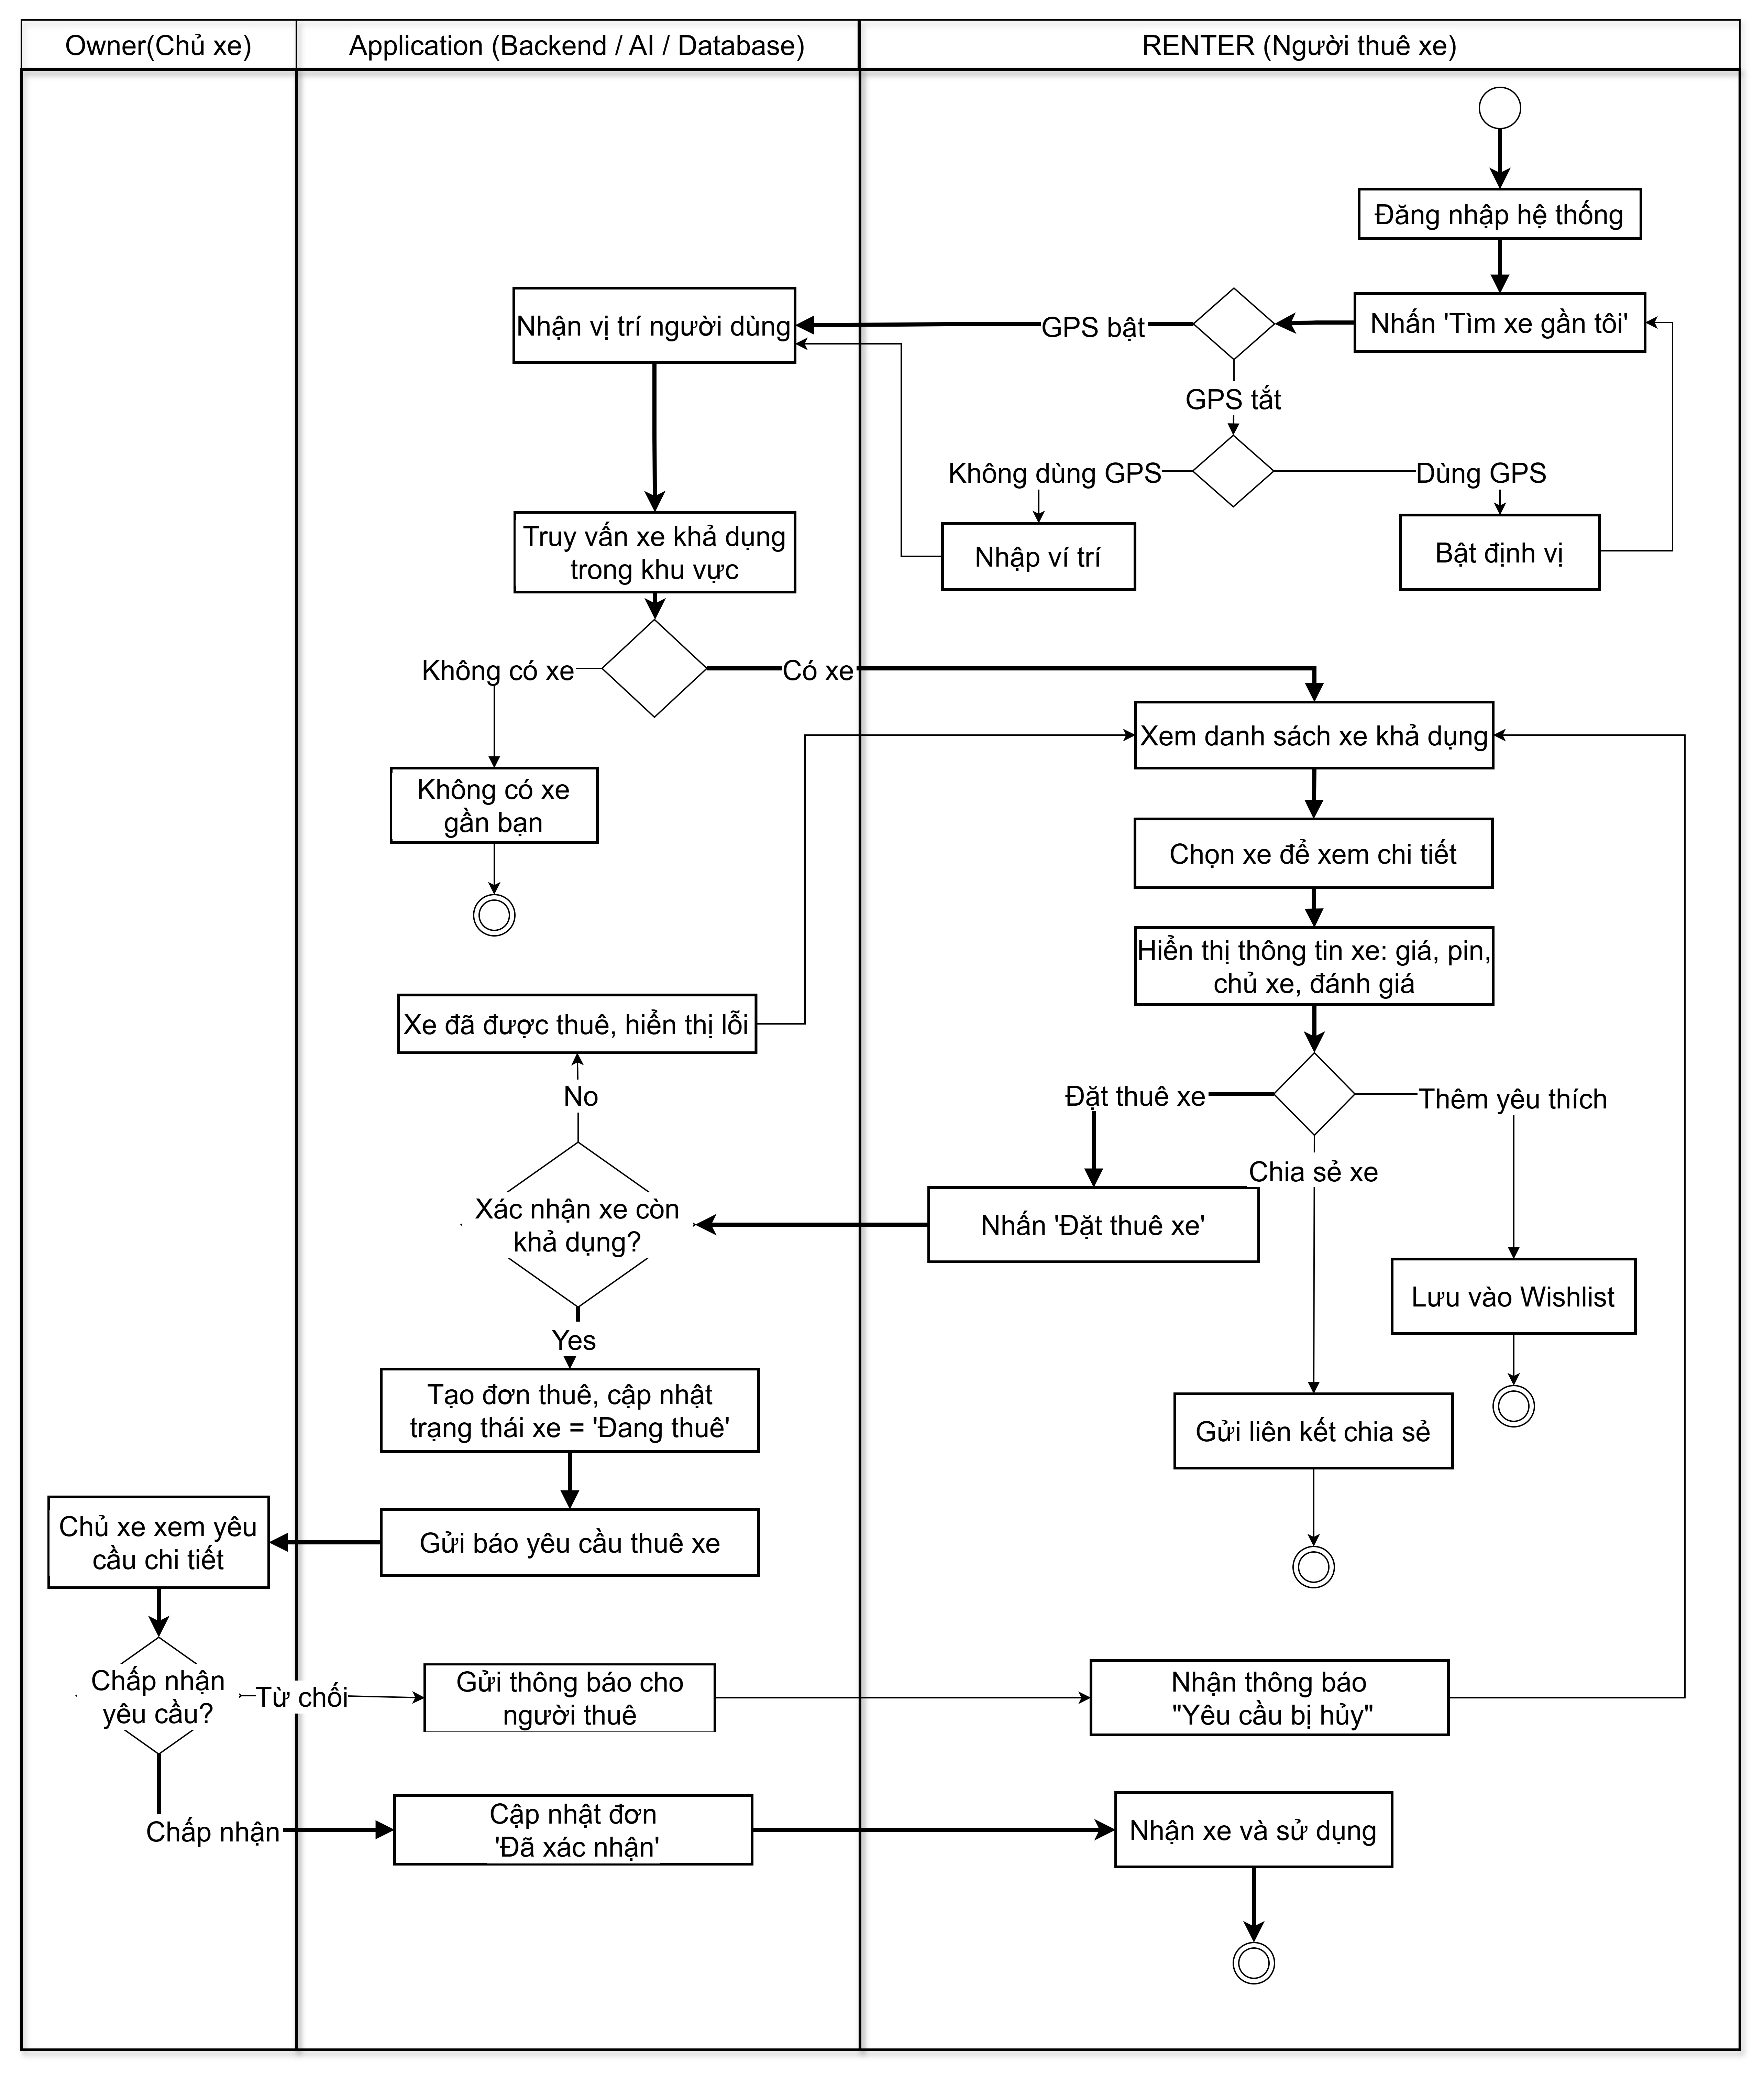
\includegraphics[width=1\textwidth]{Images/Activity/rent.png}
    \caption{Renting Activity Diagram}
    \label{fig:rent-activity}
\end{figure}

\begin{figure}[H]
    \centering
    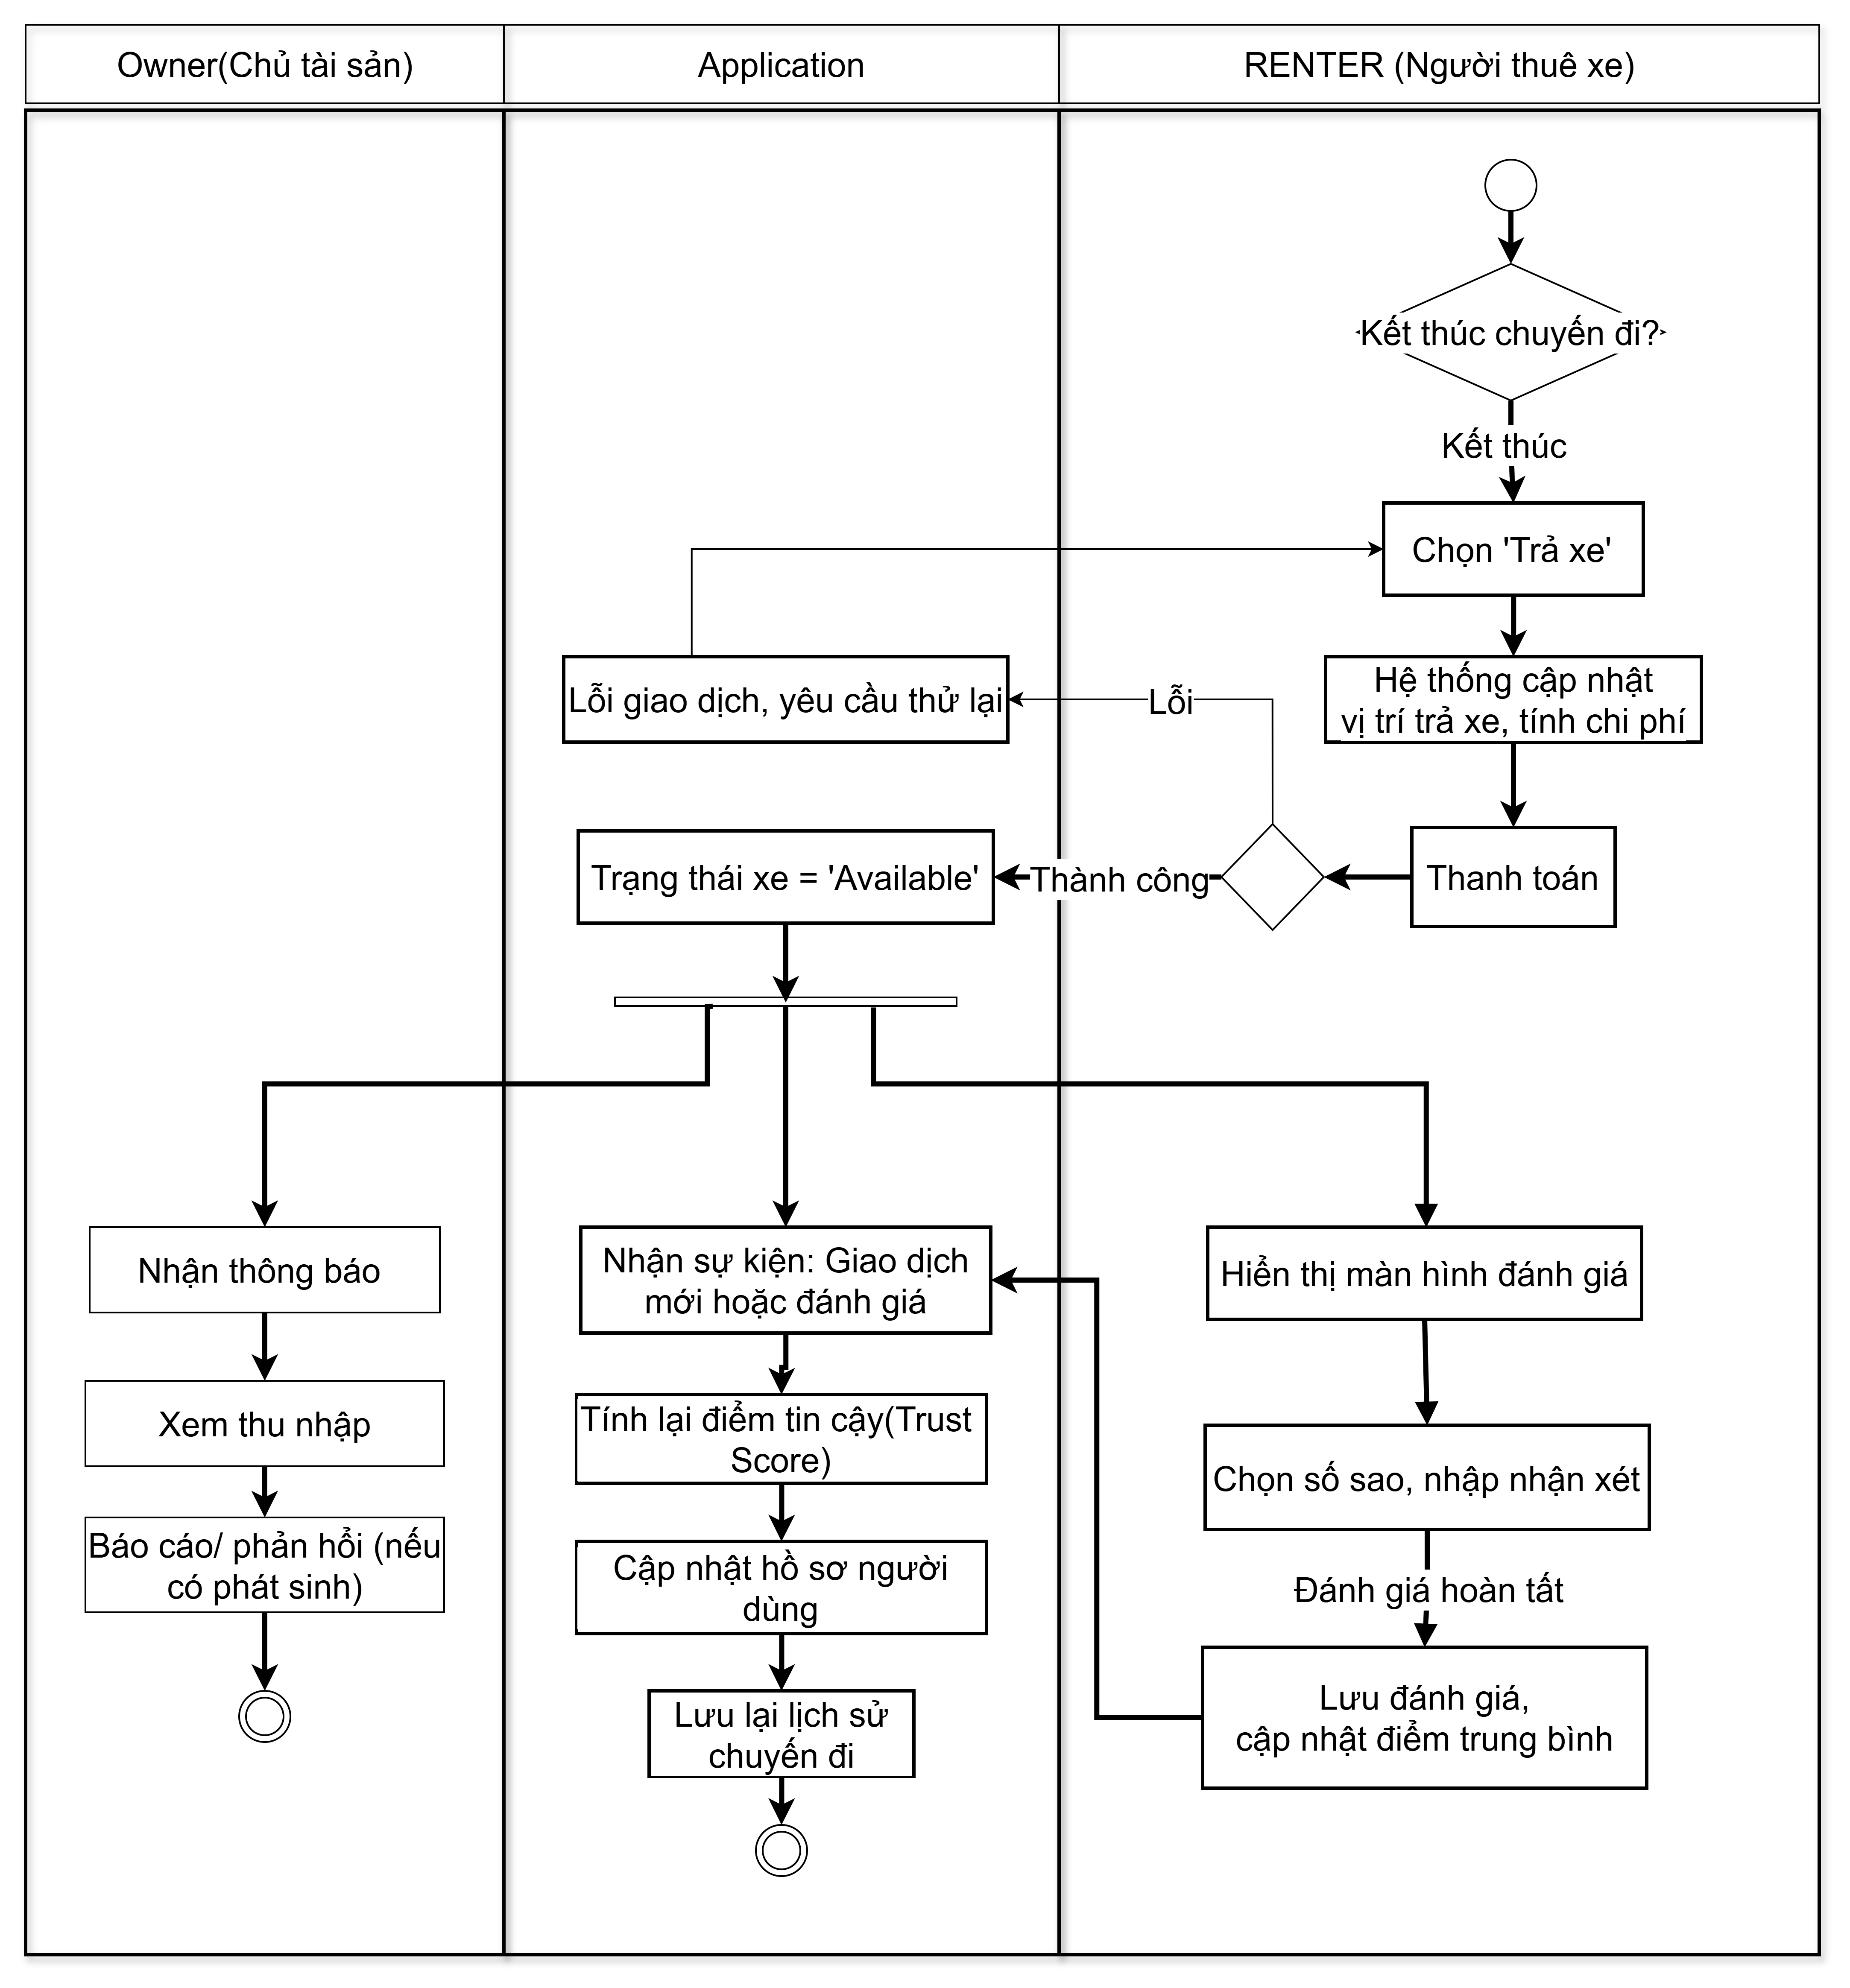
\includegraphics[width=1\textwidth]{Images/Activity/return.png}
    \caption{Returning Activity Diagram}
    \label{fig:return-activity}
\end{figure}

% ---------------------- REGISTER VEHICLE ----------------------
\subsubsection{Quy trình đăng ký xe cho thuê (UC-08)}
\label{subsec:regis-activity}
\small\textit{(Hình \ref{fig:regis-activity})}
\subsubsection*{Mục tiêu:}
Cho phép chủ xe thêm phương tiện của mình vào hệ thống để chia sẻ hoặc cho thuê, đảm bảo thông tin được xác thực và duyệt bởi quản trị viên trước khi hoạt động.
\subsubsection*{Actor chính: Chủ xe (Owner)}
\begin{figure}[H]
    \centering
    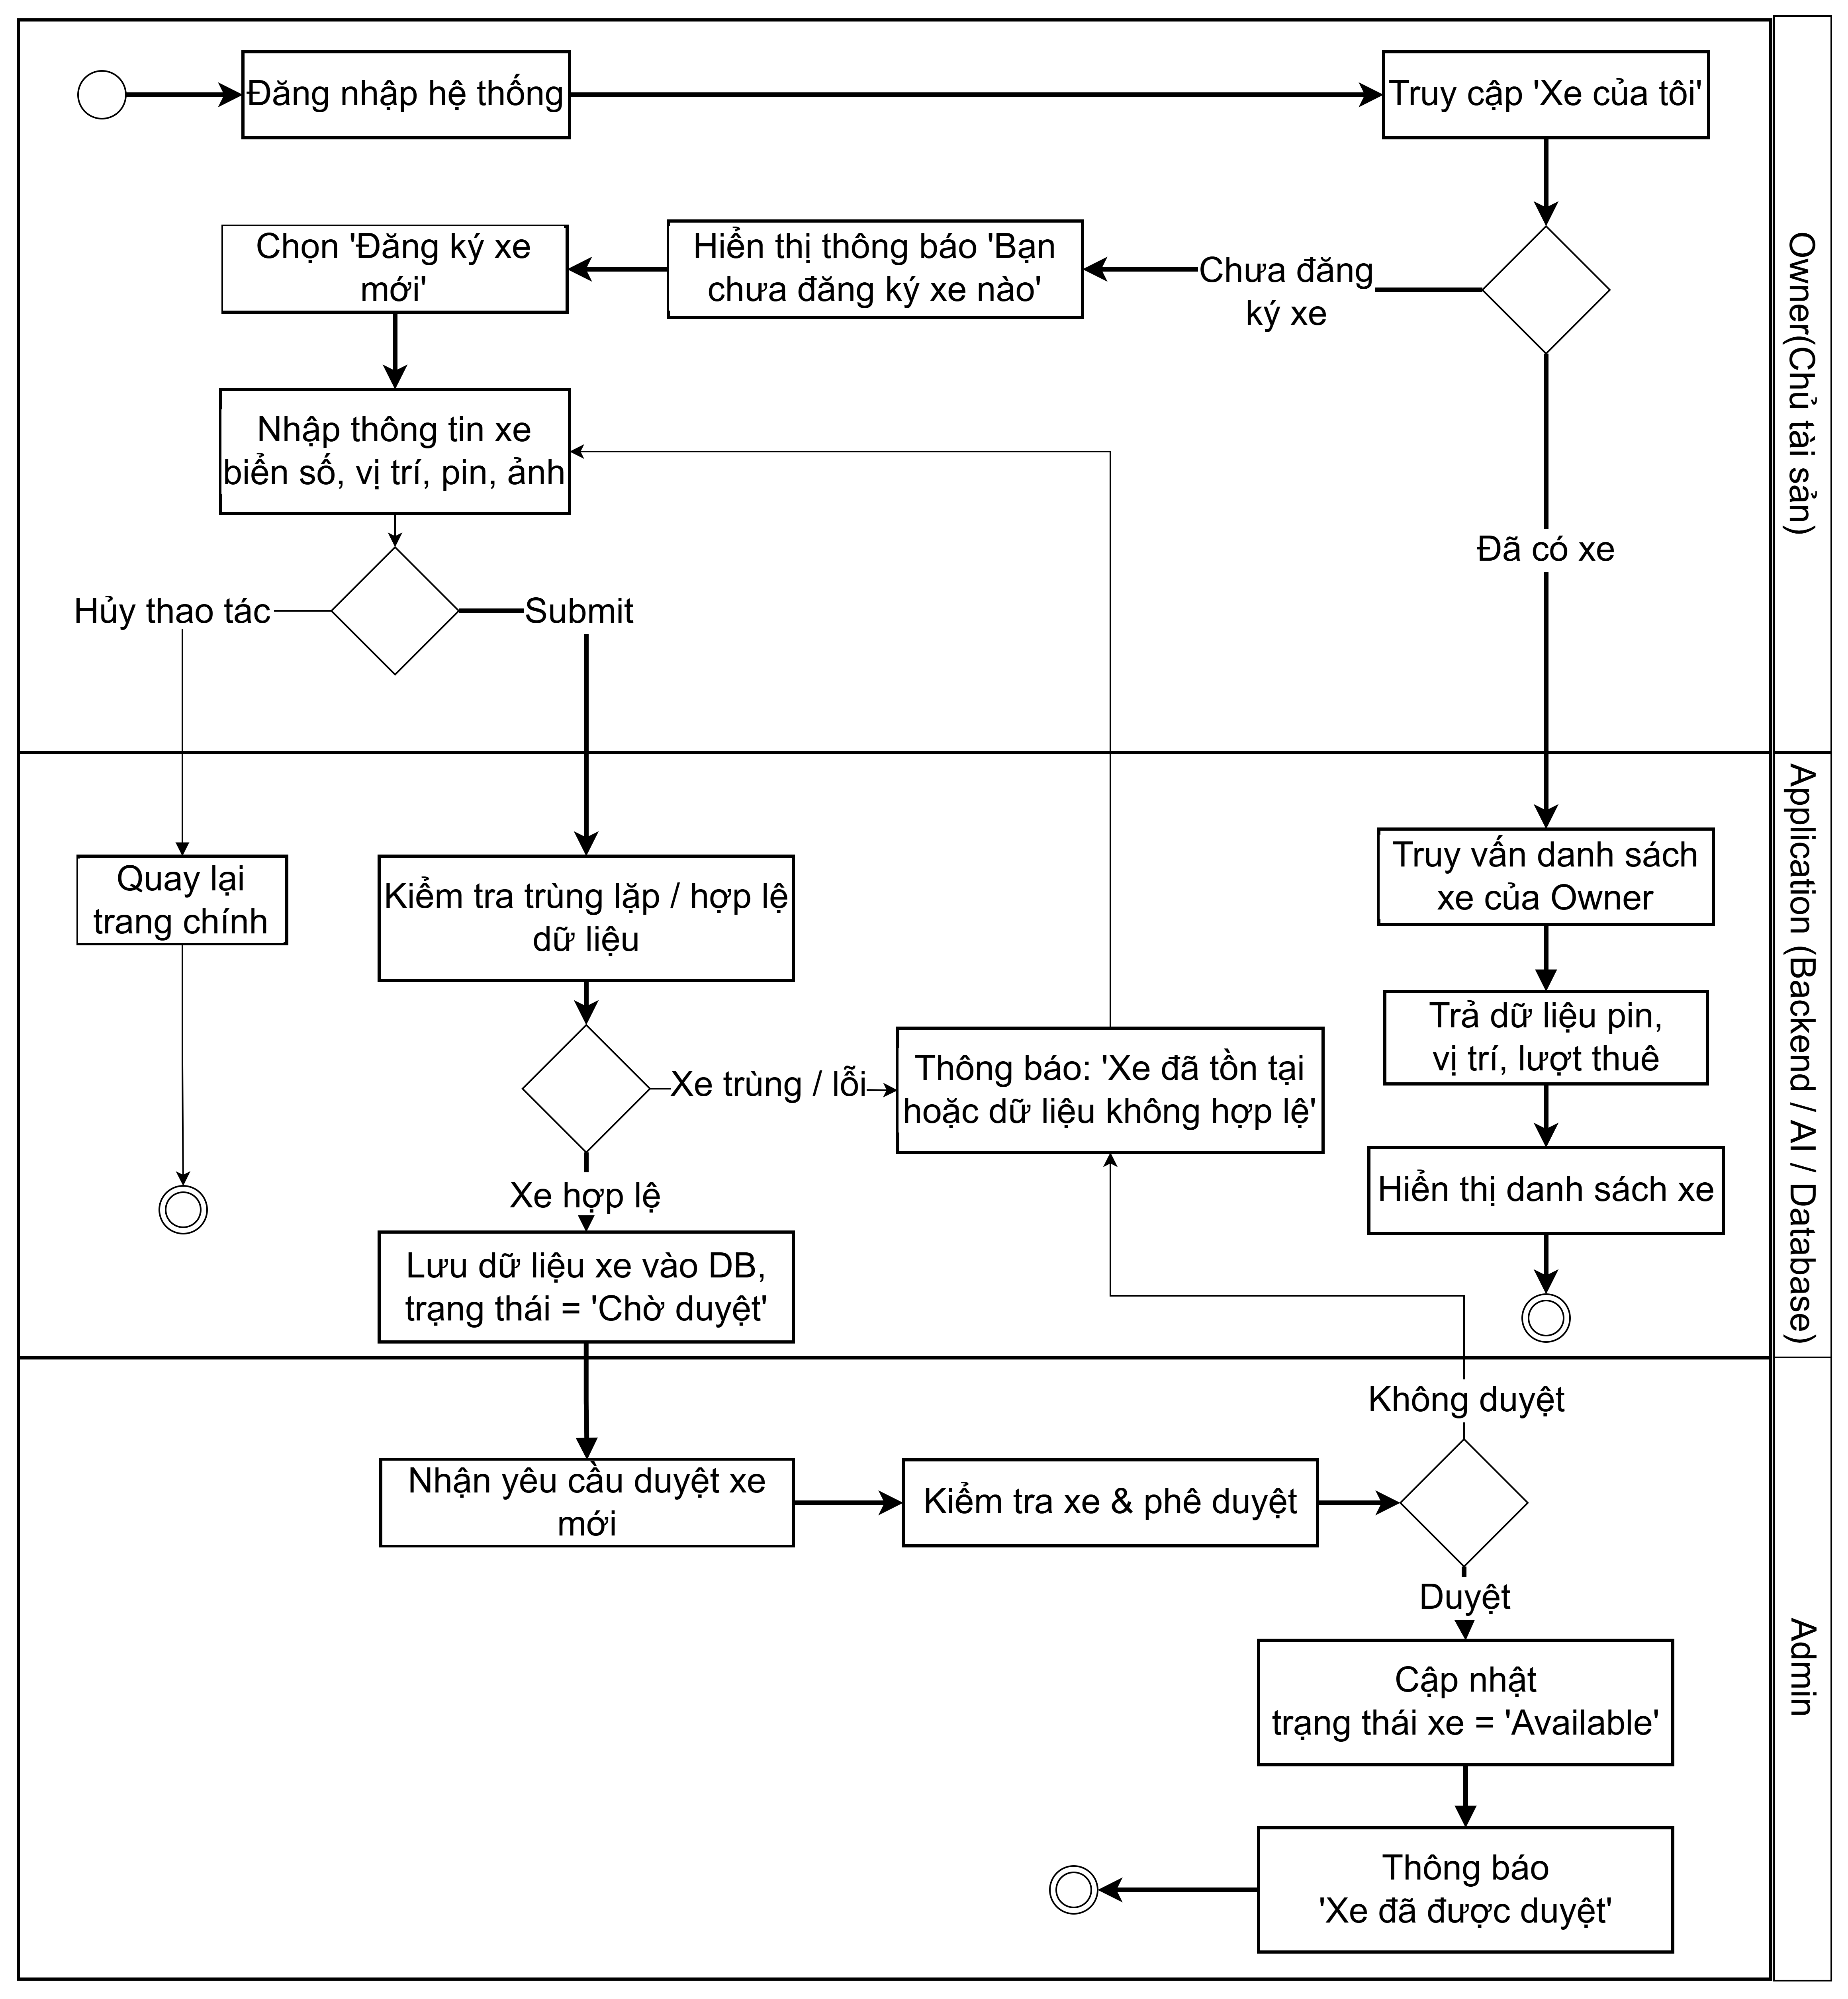
\includegraphics[width=1\textwidth]{Images/Activity/submit.png}
    \caption{Register Vehicle Activity Diagram}
    \label{fig:regis-activity}
\end{figure}
\subsubsection*{Các bước chính:}
1. Chủ xe đăng nhập và chọn chức năng “Đăng ký xe cho thuê”. \newline
2. Hệ thống hiển thị biểu mẫu để nhập thông tin xe: biển số, model, dung lượng pin, giá thuê, vị trí và hình ảnh. \newline
3. Chủ xe nhập thông tin và gửi yêu cầu đăng ký. \newline
4. Hệ thống kiểm tra dữ liệu hợp lệ (trùng biển số, định dạng ảnh, thông tin bắt buộc). \newline
5. Nếu hợp lệ, hệ thống tạo bản ghi xe mới trong cơ sở dữ liệu với trạng thái “Chờ duyệt (Pending)”. \newline
6. Gửi thông báo đến quản trị viên để xem xét và phê duyệt. \newline
7. Sau khi được duyệt, xe chuyển sang trạng thái “Available” và sẵn sàng cho thuê.
\subsubsection*{Luồng thay thế:}
- Chủ xe có thể lưu bản nháp nếu chưa hoàn tất thông tin. \newline
- Nếu phát hiện lỗi dữ liệu (trùng biển số, ảnh sai định dạng), hệ thống hiển thị thông báo để người dùng chỉnh sửa.

% ---------------------- MANAGE VEHICLE ----------------------
\begin{figure}[H]
    \centering
    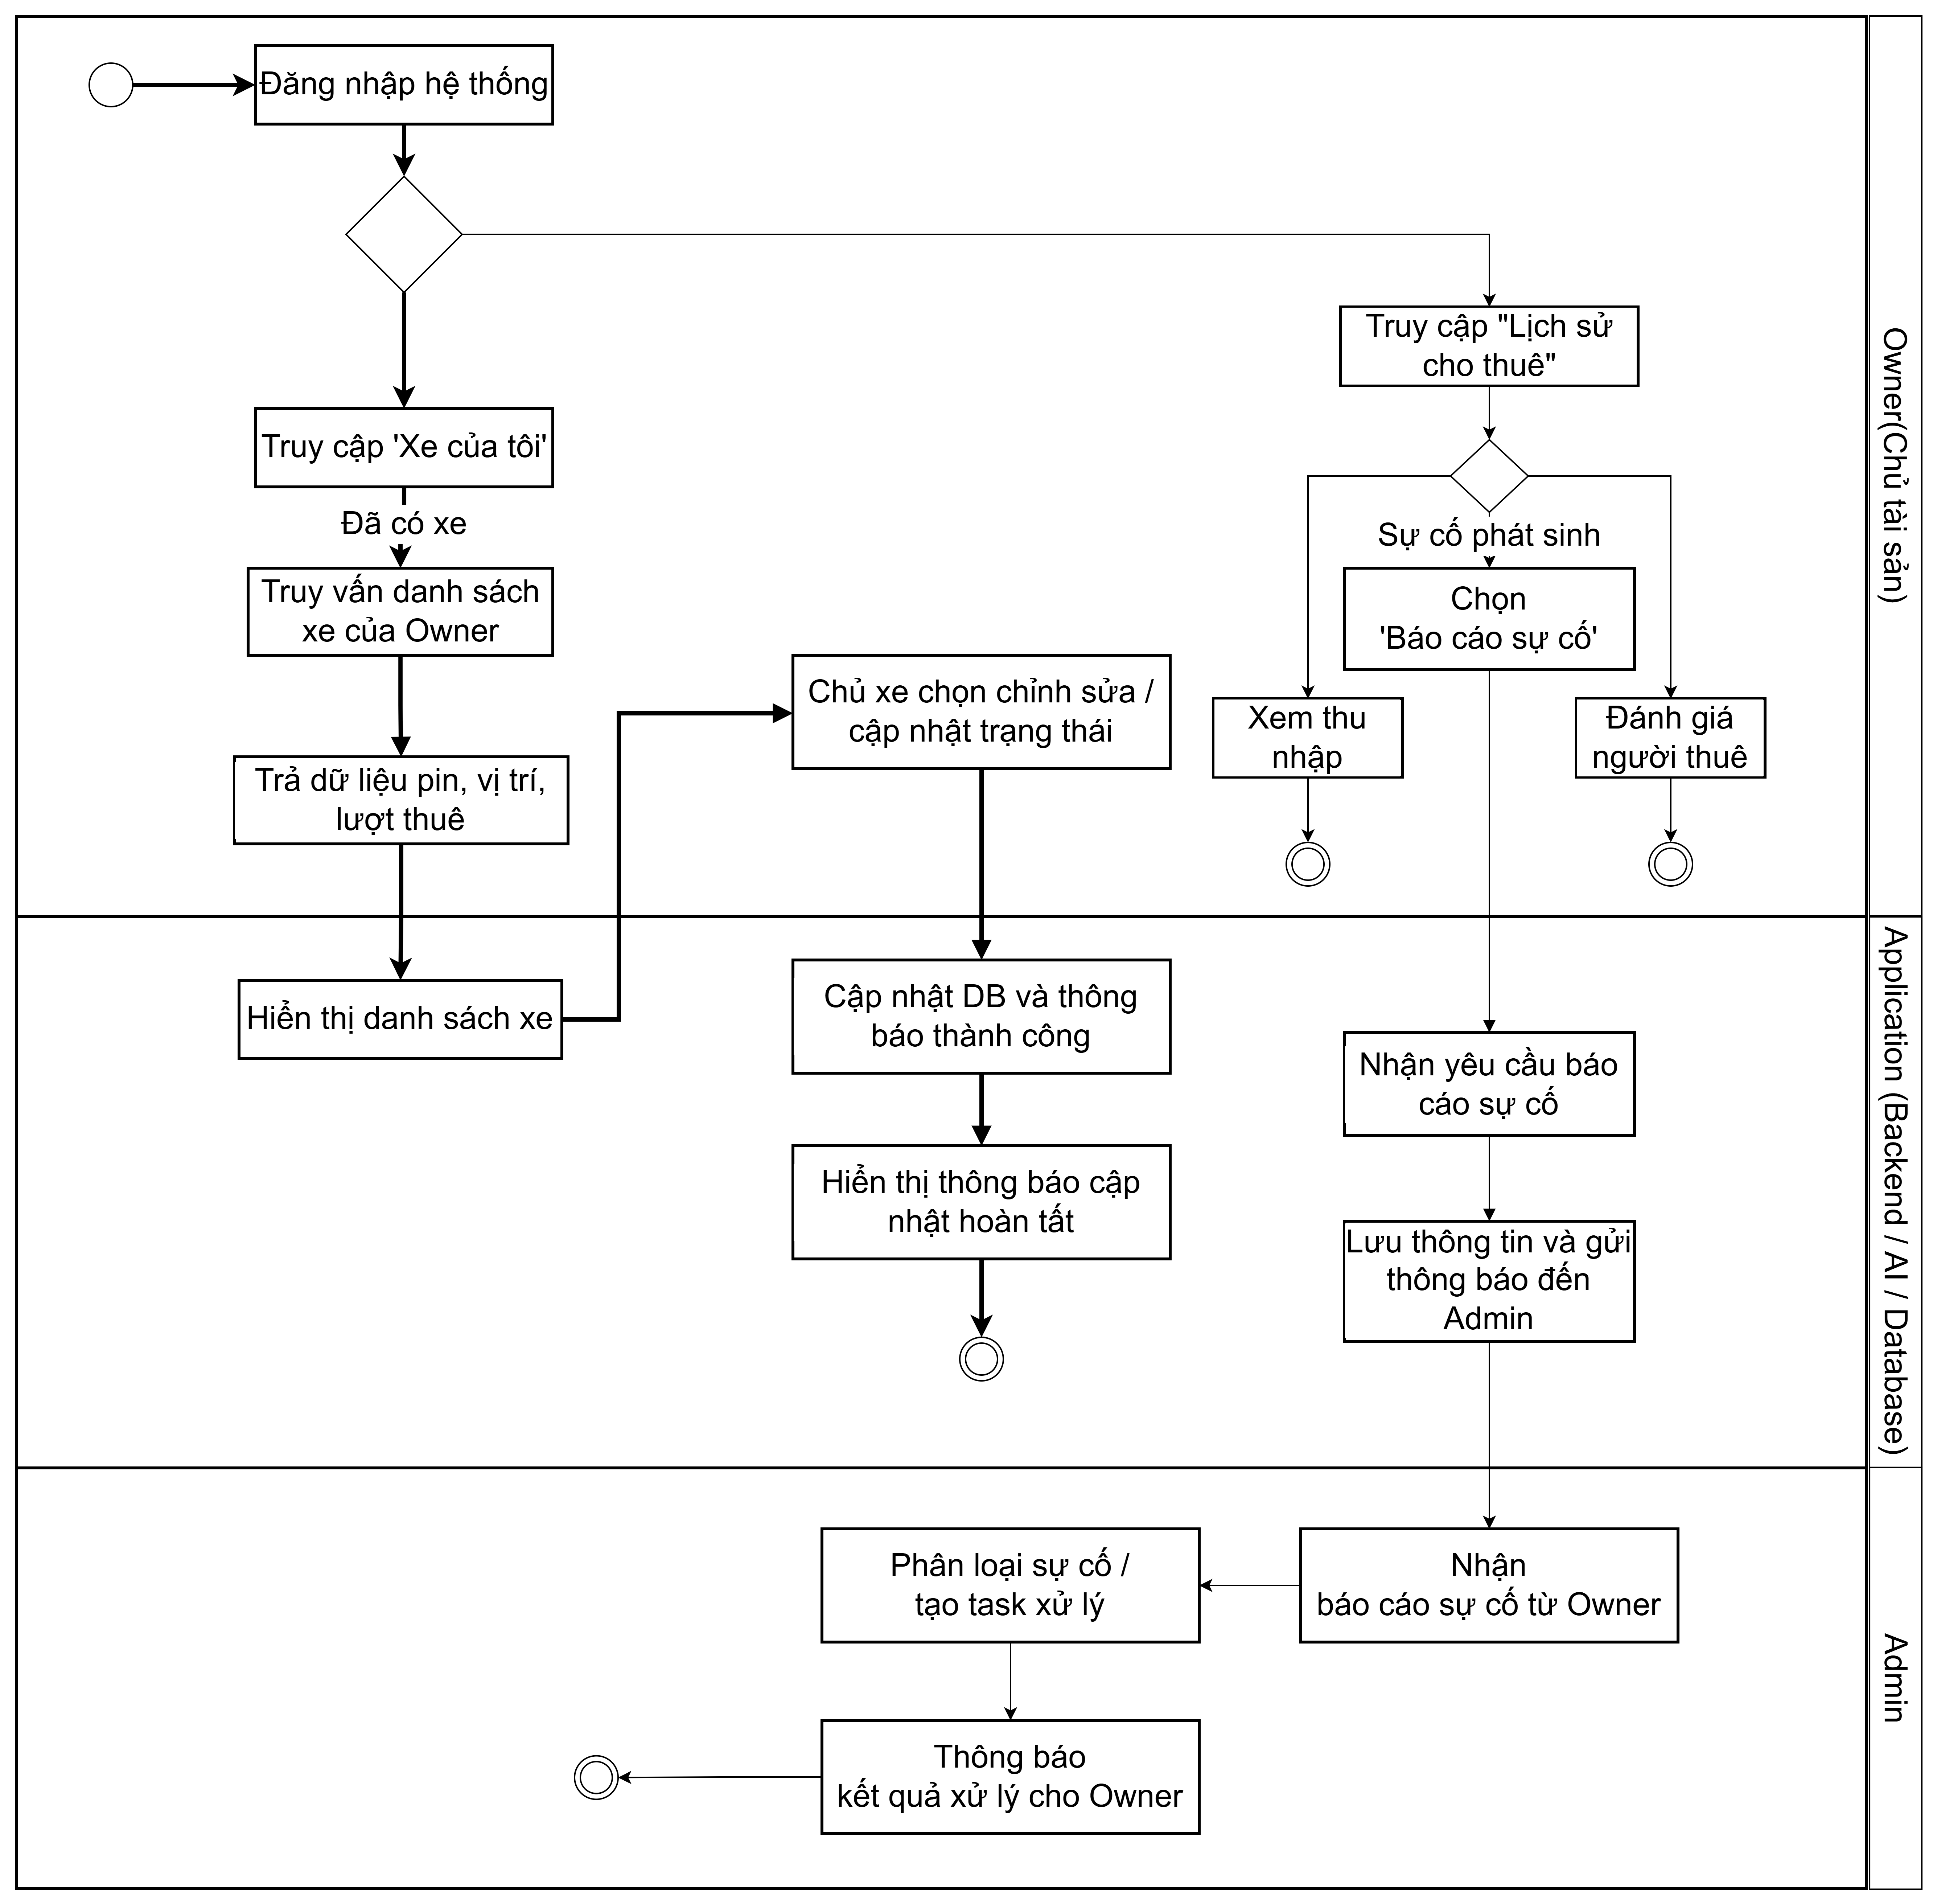
\includegraphics[width=1\textwidth]{Images/Activity/owner_management.png}
    \caption{Manage Vehicle Activity Diagram}
    \label{fig:manage-bike-activity}
\end{figure}
\subsubsection{Quy trình quản lý xe của chủ (UC-09)}
\label{subsec:manage-bike-activity}
\small\textit{(Hình \ref{fig:manage-bike-activity})}
\subsubsection*{Mục tiêu:}
Cho phép chủ xe theo dõi, cập nhật và quản lý các xe đã đăng ký cho thuê, đảm bảo thông tin xe luôn chính xác và đồng bộ với hệ thống.
\subsubsection*{Actor chính: Chủ xe (Owner)}
\subsubsection*{Các bước chính:}
1. Chủ xe đăng nhập và chọn mục “Quản lý xe”. \newline
2. Hệ thống hiển thị danh sách tất cả xe mà chủ xe đã đăng ký. \newline
3. Chủ xe chọn một xe để xem thông tin chi tiết. \newline
4. Thực hiện các thao tác: cập nhật giá, trạng thái pin, vị trí, hoặc tạm ẩn xe khỏi danh sách cho thuê. \newline
5. Hệ thống xác nhận và lưu thay đổi vào cơ sở dữ liệu. \newline
6. Các thay đổi được đồng bộ và phản ánh lên bản đồ xe cho thuê.
\subsubsection*{Luồng thay thế:}
- Chủ xe có thể kích hoạt cập nhật vị trí tự động qua GPS. \newline
- Xe đang cho thuê không thể bị ẩn hoặc xóa khỏi hệ thống cho đến khi kết thúc hành trình.

% ---------------------- ADMIN PROCESS ----------------------
\subsubsection{Quy trình quản trị hệ thống (UC-10, UC-11, UC-12)}
\label{subsec:admin-activity}
\small\textit{(Hình \ref{fig:admin-activity})}
\subsubsection*{Mục tiêu:}
Đảm bảo nền tảng hoạt động ổn định, an toàn và minh bạch thông qua việc kiểm duyệt xe, quản lý người dùng, và theo dõi hiệu quả hoạt động chung của hệ thống.
\subsubsection*{Actor chính: Quản trị viên (Admin)}
\subsubsection*{Các bước chính:}
1. Admin đăng nhập vào hệ thống quản trị. \newline
2. Hệ thống hiển thị bảng điều khiển (Dashboard) với các module: \textit{Duyệt xe}, \textit{Quản lý người dùng}, \textit{Báo cáo - Thống kê}. \newline
3. Admin chọn module cần thao tác:
3.1. \textbf{Duyệt xe:} Xem danh sách xe chờ duyệt, kiểm tra thông tin, hình ảnh, giấy tờ → phê duyệt hoặc từ chối → hệ thống cập nhật trạng thái và gửi thông báo cho chủ xe.\\
3.2. \textbf{Quản lý người dùng:} Xem danh sách người dùng, khóa/mở khóa tài khoản, thay đổi quyền truy cập (User, Owner, Admin), gửi cảnh cáo cho người vi phạm.\\
3.3. \textbf{Báo cáo - Thống kê:} Chọn loại báo cáo (doanh thu, lượt thuê, hoạt động theo khu vực), hệ thống tổng hợp dữ liệu, hiển thị biểu đồ và cho phép xuất file (PDF, Excel).\\
4. Sau khi hoàn tất thao tác, hệ thống lưu lại log quản trị (audit trail) để theo dõi thay đổi. \newline
5. Quản trị viên có thể đăng xuất hoặc chuyển sang module khác mà không ảnh hưởng dữ liệu.
\subsubsection*{Luồng thay thế:}
- Nếu dữ liệu bị lỗi hoặc chậm cập nhật, hệ thống hiển thị thông báo “Dữ liệu đang đồng bộ”. \newline
- Khi không đủ quyền thao tác, hiển thị cảnh báo “Không đủ quyền truy cập”. \newline
- Admin có thể lọc dữ liệu hoặc thay đổi thời gian xem thống kê linh hoạt.

% ---------------------- FIGURES ----------------------
\begin{figure}[H]
    \centering
    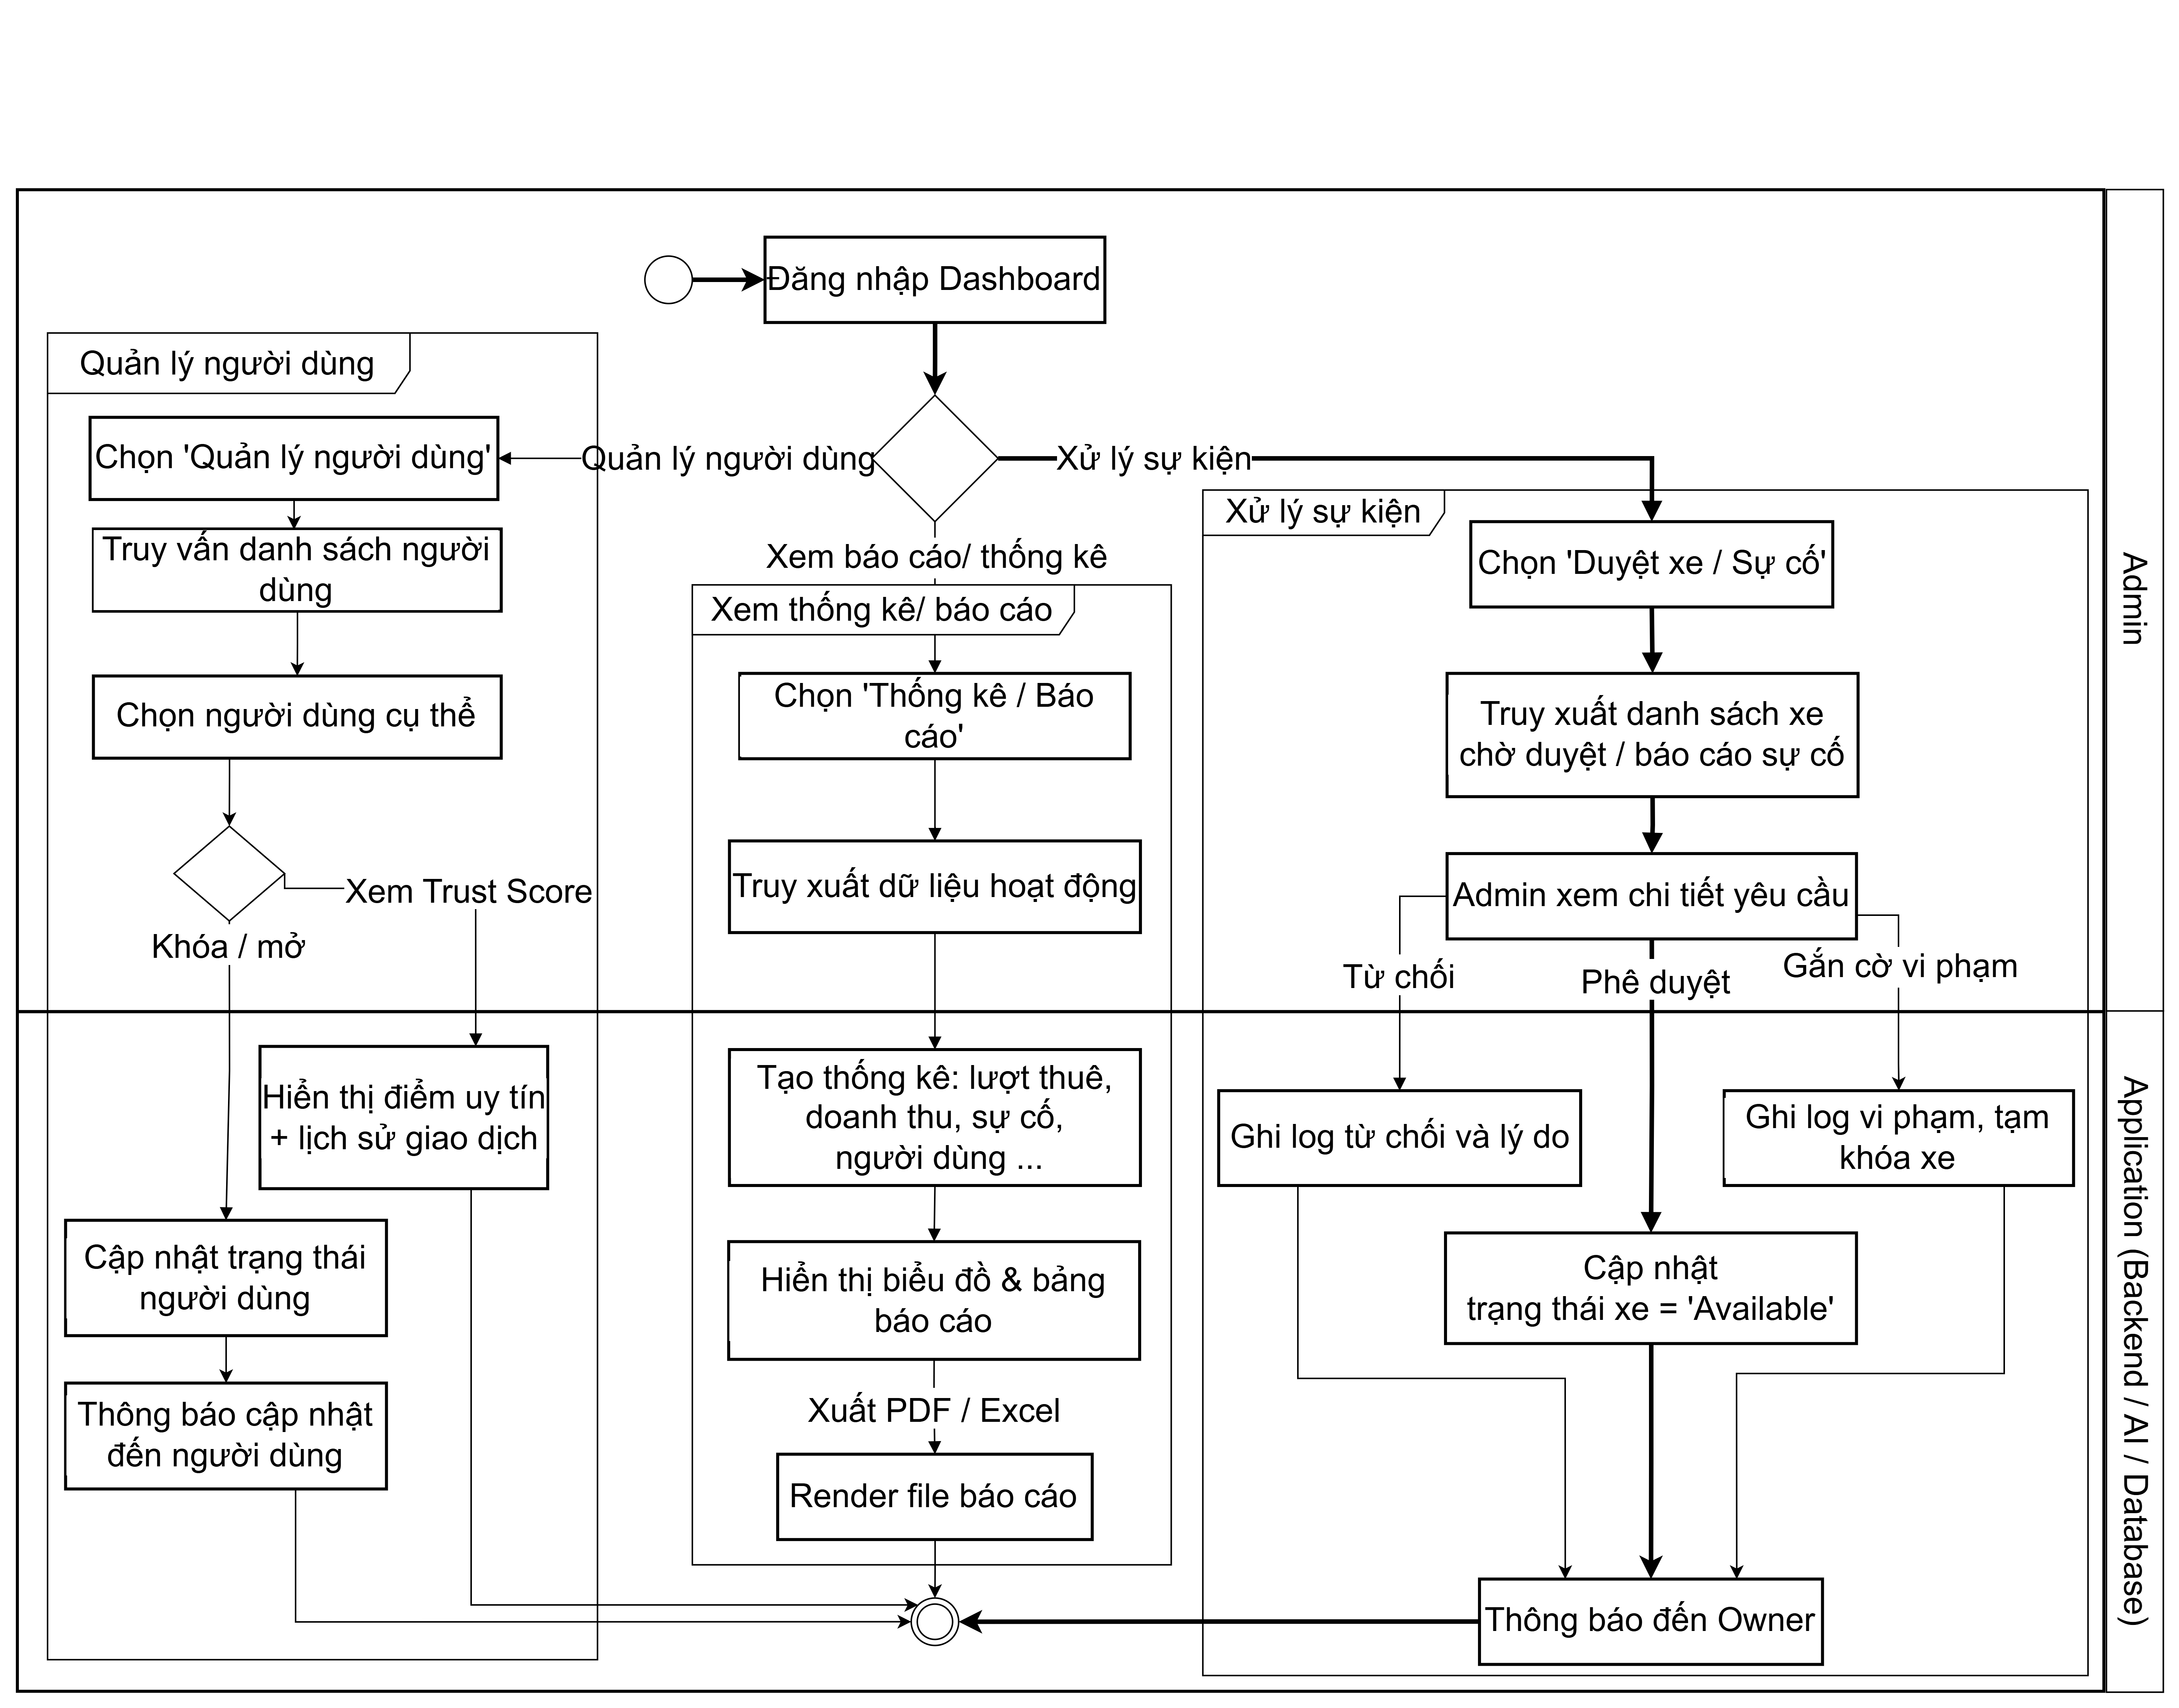
\includegraphics[width=1\textwidth]{Images/Activity/admin.png}
    \caption{Administrative Action Activity Diagram}
    \label{fig:admin-activity}
\end{figure}

\newpage
\subsection{Mô hình hóa hành vi hệ thống}

\subsection*{Renter Flow}

\subsubsection{Tìm và Đặt thuê xe (UC-02, UC-03, UC-04) \small\textit{(Hình \ref{fig:rent-sequence})}}
\subsubsection*{Mô tả tổng quát}
Người thuê tìm kiếm xe điện gần vị trí hiện tại, xem chi tiết và tiến hành đặt thuê.

\subsubsection*{Thành phần và vai trò}
1. \textbf{Renter:} Khởi tạo yêu cầu tìm xe, xem chi tiết, đặt thuê \\
2. \textbf{MobileApp:} Giao diện và trung gian gửi yêu cầu \\
3. \textbf{RentalController:} Xử lý logic chính, điều phối các dịch vụ \\
4. \textbf{VehicleService:} Cung cấp dữ liệu xe khả dụng \\
5. \textbf{NotificationService:} Gửi thông báo xác nhận cho chủ xe \\
6. \textbf{Database:} Lưu trữ thông tin xe và đơn thuê

\subsubsection*{Hành vi hệ thống}
1. Người thuê chọn "Tìm xe gần tôi", app gửi yêu cầu vị trí GPS. \\
2. RentalController gọi VehicleService truy vấn danh sách xe khả dụng trong bán kính. \\
3. Kết quả hiển thị trên bản đồ, người thuê chọn 1 xe để xem chi tiết. \\
4. Khi nhấn "Đặt thuê", hệ thống kiểm tra tình trạng xe, ghi nhận đơn trong Database, gửi notification đến chủ xe. \\
5. Nếu xe bận hoặc mạng lỗi → hiển thị thông báo lỗi. \\
6. Người thuê có thể chỉnh sửa thời gian thuê trước khi chủ xe xác nhận.

\subsubsection{Theo dõi chuyến đi}

\subsubsection*{Mô tả tổng quát}
Hệ thống giám sát hành trình, pin và chi phí theo thời gian thực trong khi xe đang được thuê.

\subsubsection*{Thành phần và vai trò}
1. \textbf{Renter:} Theo dõi hành trình \\
2. \textbf{MobileApp:} Hiển thị bản đồ, đồng bộ dữ liệu \\
3. \textbf{RentalController:} Xử lý truy vấn trạng thái \\
4. \textbf{VehicleService:} Cập nhật thông tin xe \\
5. \textbf{Database:} Lưu dữ liệu vị trí, pin, chi phí

\subsubsection*{Hành vi hệ thống}
1. Sau khi chủ xe chấp nhận, booking chuyển sang active. \\
2. App gửi yêu cầu cập nhật trạng thái định kỳ (polling mỗi 10s). \\
3. Hệ thống lấy dữ liệu vị trí, pin, thời gian, chi phí từ DB. \\
4. App hiển thị hành trình theo thời gian thực. \\
5. Khi pin < 20\% → gửi cảnh báo cho người dùng. \\
6. Nếu lỗi GPS → cho phép nhập vị trí thủ công.

\subsubsection{Kết thúc chuyến đi \& Đánh giá (UC-05, UC-06, UC-07) \small\textit{(Hình \ref{fig:return-sequence})}}

\subsubsection*{Mô tả tổng quát}
Người thuê kết thúc hành trình, hệ thống thực hiện thanh toán tự động và hiển thị giao diện đánh giá chủ xe.

\subsubsection*{Thành phần và vai trò}
1. \textbf{Renter:} Kết thúc chuyến đi và thực hiện đánh giá \\
2. \textbf{MobileApp:} Giao diện thanh toán và đánh giá \\
3. \textbf{RentalController:} Quản lý kết thúc thuê và xử lý logic \\
4. \textbf{VehicleService:} Cập nhật trạng thái xe về khả dụng \\
5. \textbf{PaymentService:} Tính toán và xử lý thanh toán \\
6. \textbf{NotificationService:} Gửi thông báo hoàn tất và cập nhật TrustScore \\
7. \textbf{Database:} Lưu thanh toán và đánh giá

\subsubsection*{Hành vi hệ thống}
1. Renter nhấn "Kết thúc chuyến đi". \\
2. RentalController cập nhật trạng thái xe về available qua VehicleService. \\
3. PaymentService tính chi phí dựa trên thời gian và mức giá, thực hiện thanh toán. \\
4. Nếu thanh toán thành công → lưu kết quả và gửi thông báo hoàn tất đến Renter \& Owner. \\
5. App hiển thị giao diện đánh giá sau thuê. \\
6. Người thuê có thể: \\
\quad (a) Chấm sao và viết bình luận → lưu vào DB, cập nhật TrustScore. \\
\quad (b) Chỉ chấm sao → lưu tối giản. \\
\quad (c) Bỏ qua → đánh dấu review pending. \\
7. Nếu mất mạng → dữ liệu được lưu tạm và gửi lại khi có kết nối.

\begin{figure}[H]
    \centering
    \includegraphics[width=0.95\textwidth]{Images/Sequence/rent.png}
    \caption{Sequence Diagram - Tìm và Đặt thuê xe}
    \label{fig:rent-sequence}
\end{figure}

\begin{figure}[H]
    \centering
    \includegraphics[width=0.95\textwidth]{Images/Sequence/return.png}
    \caption{Sequence Diagram - Kết thúc chuyến đi \& Đánh giá}
    \label{fig:return-sequence}
\end{figure}

\subsection*{Owner Flow}
\subsubsection{Đăng ký xe cho thuê (UC-08) \small\textit{(Hình \ref{fig:regis-sequence})}}

\subsubsection*{Mô tả tổng quát}
Chức năng cho phép chủ xe đăng ký phương tiện mới để đưa lên hệ thống cho thuê. Quá trình này yêu cầu xác nhận từ Admin trước khi xe được kích hoạt.
\subsubsection*{Thành phần và vai trò}
1. \textbf{Owner:} Nhập thông tin và gửi yêu cầu đăng ký xe \\
2. \textbf{OwnerApp:} Giao diện nhập và gửi dữ liệu xe \\
3. \textbf{VehicleController:} Xử lý yêu cầu đăng ký, giao tiếp với DB và hệ thống duyệt \\
4. \textbf{Database:} Lưu thông tin xe với trạng thái "pending" \\
5. \textbf{AdminSystem:} Duyệt hoặc từ chối xe đăng ký \\
6. \textbf{NotificationService:} Gửi thông báo về kết quả duyệt

\begin{figure}[H]
    \centering
    \includegraphics[width=0.9\textwidth]{Images/Sequence/regis.png}
    \caption{Sequence Diagram - Đăng ký xe cho thuê}
    \label{fig:regis-sequence}
\end{figure}

\subsubsection*{Hành vi hệ thống}
1. Owner nhập thông tin xe (ảnh, vị trí, giá, loại, pin). \\
2. OwnerApp gửi yêu cầu đến VehicleController → ghi vào Database với trạng thái pending. \\
3. VehicleController gửi yêu cầu duyệt đến AdminSystem. \\
4. Khi Admin phê duyệt: hệ thống cập nhật trạng thái xe thành available và NotificationService gửi thông báo "Xe đã được duyệt". \\
5. Nếu bị từ chối: hiển thị lý do cho Owner. \\
6. Nếu lỗi mạng khi gửi, dữ liệu được lưu tạm và đồng bộ khi có kết nối lại.

\subsubsection{Quản lý xe (UC-09) \small\textit{(Hình \ref{fig:manage-sequence})}}

\subsubsection*{Mô tả tổng quát}
Cho phép chủ xe xem, cập nhật và theo dõi tình trạng xe trong danh mục của mình.

\begin{figure}[H]
    \centering
    \includegraphics[width=0.95\textwidth]{Images/Sequence/manage.png}
    \caption{Sequence Diagram - Quản lý xe}
    \label{fig:manage-sequence}
\end{figure}

\subsubsection*{Thành phần và vai trò}
1. \textbf{Owner:} Xem danh sách xe, chỉnh sửa thông tin \\
2. \textbf{OwnerApp:} Hiển thị danh sách và giao diện cập nhật \\
3. \textbf{VehicleController:} Điều phối truy vấn và cập nhật dữ liệu \\
4. \textbf{VehicleService:} Cung cấp trạng thái xe (pin, vị trí, đánh giá) \\
5. \textbf{Database:} Lưu và cập nhật thông tin xe \\
6. \textbf{NotificationService:} Thông báo cho Renter nếu có thay đổi ảnh hưởng

\subsubsection*{Hành vi hệ thống}
1. OwnerApp gửi yêu cầu xem danh sách xe → VehicleController truy vấn DB. \\
2. Owner có thể chọn xem chi tiết 1 xe → lấy dữ liệu từ VehicleService (pin, vị trí, điểm đánh giá). \\
3. Khi Owner cập nhật trạng thái hoặc giá: \\
\quad - Nếu hợp lệ → DB cập nhật thành công và hiển thị thông báo. \\
\quad - Nếu xe đang được thuê → từ chối thay đổi, hiển thị cảnh báo. \\
4. Nếu có booking đang hoạt động, NotificationService gửi thông báo đến Renter. \\
5. Khi mất kết nối, app hiển thị dữ liệu cache cũ và đồng bộ khi có mạng.

\subsubsection{Báo cáo sự cố (UC-16) \small\textit{(Hình \ref{fig:accident-sequence})}}

\subsubsection*{Mô tả tổng quát}
Hỗ trợ chủ xe báo cáo vấn đề liên quan đến xe, hành vi thuê, hoặc sự cố kỹ thuật.
\subsubsection*{Thành phần và vai trò}
1. \textbf{Owner:} Tạo báo cáo sự cố \\
2. \textbf{OwnerApp:} Gửi yêu cầu báo cáo \\
3. \textbf{VehicleController:} Ghi nhận và gửi báo cáo đến Admin \\
4. \textbf{Database:} Lưu trạng thái và log báo cáo \\
5. \textbf{AdminSystem:} Tiếp nhận và xác nhận xử lý \\
6. \textbf{NotificationService:} Gửi phản hồi lại cho chủ xe
\subsubsection*{Hành vi hệ thống}
1. Owner nhập mô tả sự cố và gửi đến VehicleController. \\
2. Hệ thống lưu báo cáo (pending) và gửi lên AdminSystem để xử lý. \\
3. Khi Admin phản hồi → cập nhật trạng thái acknowledged trong DB và thông báo cho Owner. \\
4. Nếu timeout hoặc không phản hồi → hiển thị lỗi, cho phép gửi lại.
\begin{figure}[H]
    \centering
    \includegraphics[width=1\textwidth]{Images/Sequence/accident.png}
    \caption{Sequence Diagram - Báo cáo sự cố}
    \label{fig:accident-sequence}
\end{figure}

\subsubsection{Thông báo hệ thống (UC-17) \small\textit{(Hình \ref{fig:notification-sequence})}}

\subsubsection*{Mô tả tổng quát}
Các thông báo push được gửi tự động từ NotificationService đến OwnerApp khi có sự kiện quan trọng.
\subsubsection*{Thành phần và vai trò}
1. \textbf{NotificationService:} Phát sinh và gửi thông báo \\
2. \textbf{OwnerApp:} Hiển thị thông báo, xử lý phản hồi \\
3. \textbf{VehicleController:} Cập nhật trạng thái khi Owner phản hồi \\
4. \textbf{AdminSystem:} Xử lý vi phạm hoặc phản hồi Owner \\
5. \textbf{Database:} Lưu log và hàng đợi thông báo
\subsubsection*{Hành vi hệ thống}
1. Khi có sự kiện như xe được duyệt, yêu cầu thuê mới, hoặc báo cáo được xử lý, NotificationService gửi push đến OwnerApp. \\
2. OwnerApp hiển thị nội dung thông báo và cho phép phản hồi. \\
3. Khi Owner phản hồi (ví dụ xác nhận booking), VehicleController cập nhật DB và gửi thông báo ngược lại cho Renter. \\
4. Nếu lỗi kết nối → NotificationService lưu thông báo vào queue để gửi lại sau.
\begin{figure}[H]
    \centering
    \includegraphics[width=1\textwidth]{Images/Sequence/notification.png}
    \caption{Sequence Diagram - Thông báo hệ thống}
    \label{fig:notification-sequence}
\end{figure}

\subsection*{Admin Flow}
\subsubsection{Duyệt xe / Quản trị hệ thống (UC-10) \small\textit{(Hình \ref{fig:admin-approve-sequence})}}
\subsubsection*{Mô tả tổng quát}
Admin chịu trách nhiệm duyệt xe mới đăng ký, xử lý xe vi phạm, và quản trị dữ liệu trong hệ thống.
\begin{figure}[H]
    \centering
    \includegraphics[width=1\textwidth]{Images/Sequence/admin_approve.png}
    \caption{Sequence Diagram - Duyệt xe / Quản trị hệ thống}
    \label{fig:admin-approve-sequence}
\end{figure}
\subsubsection*{Thành phần và vai trò}
1. \textbf{Admin:} Thực hiện duyệt xe, khóa xe, hoặc quản trị chung \\
2. \textbf{AdminDashboard:} Giao diện quản trị hiển thị danh sách xe chờ duyệt \\
3. \textbf{AdminController:} Xử lý logic duyệt xe và thao tác dữ liệu \\
4. \textbf{Database:} Lưu trữ thông tin xe và trạng thái duyệt \\
5. \textbf{NotificationService:} Gửi thông báo cho Owner khi có thay đổi

\subsubsection*{Hành vi hệ thống}
1. Admin đăng nhập vào hệ thống qua AdminDashboard. \\
2. AdminDashboard gửi yêu cầu đến AdminController để lấy danh sách xe đang chờ duyệt. \\
3. AdminController truy vấn Database để lấy các bản ghi có status="pending". \\
4. Hệ thống hiển thị danh sách xe đang chờ duyệt để Admin xem chi tiết từng xe. \\
5. Khi Admin chọn một xe, AdminDashboard gửi yêu cầu lấy chi tiết xe đến AdminController. \\
6. AdminController truy vấn Database để lấy thông tin xe và chủ xe tương ứng. \\
7. Admin xem thông tin chi tiết (loại xe, hình ảnh, pin, vị trí, lịch sử của Owner). \\
8. Admin chọn "Phê duyệt" hoặc "Từ chối". \\
9. \\
\quad - Nếu phê duyệt: AdminController cập nhật Database status="available" và thông báo cho Owner qua NotificationService. \\
\quad - Nếu từ chối: AdminController cập nhật status="rejected" kèm lý do, gửi thông báo từ chối đến Owner. \\
10. AdminDashboard hiển thị kết quả xử lý cho Admin. \\
11. Trường hợp có lỗi kết nối Database, hệ thống thông báo lỗi trên giao diện. \\
12. (Mở rộng) Nếu Admin phát hiện xe vi phạm, Admin có thể chọn "Khóa xe", hệ thống cập nhật status="locked" và gửi thông báo cảnh báo cho Owner.

\subsubsection{Xem báo cáo / Thống kê (UC-11) \small\textit{(Hình \ref{fig:admin-statistic-sequence})}}

\subsubsection*{Mô tả tổng quát}
Admin có thể xem thống kê tổng hợp hệ thống (doanh thu, số lượt thuê, sự cố, tỷ lệ loại xe) theo khoảng thời gian.

\subsubsection*{Thành phần và vai trò}
1. \textbf{Admin:} Chọn khoảng thời gian, xuất báo cáo \\
2. \textbf{AdminDashboard:} Giao diện hiển thị biểu đồ thống kê \\
3. \textbf{AnalyticsService:} Tổng hợp và xử lý dữ liệu thống kê \\
4. \textbf{Database:} Cung cấp dữ liệu thô (booking, report, revenue)
\begin{figure}[H]
    \centering
    \includegraphics[width=1\textwidth]{Images/Sequence/admin_statistic.png}
    \caption{Sequence Diagram - Xem báo cáo / Thống kê}
    \label{fig:admin-statistic-sequence}
\end{figure}
\subsubsection*{Hành vi hệ thống}
1. Admin chọn mục "Báo cáo \& Thống kê" trên AdminDashboard. \\
2. Admin nhập khoảng thời gian cần thống kê (startDate, endDate). \\
3. AdminDashboard gửi yêu cầu đến AnalyticsService để tạo báo cáo. \\
4. AnalyticsService truy vấn Database để lấy: \\
\quad - Tổng số lượt thuê xe, doanh thu. \\
\quad - Số lượng sự cố báo cáo. \\
\quad - Phân bố loại xe được thuê. \\
5. AnalyticsService tổng hợp và định dạng dữ liệu thành biểu đồ, số liệu thống kê, xu hướng. \\
6. Hệ thống hiển thị báo cáo trực quan cho Admin. \\
7. (Mở rộng) Nếu Admin muốn xuất file, chọn "Xuất báo cáo PDF", AnalyticsService tạo file PDF và gửi về dashboard để tải xuống. \\
8. Nếu không có dữ liệu trong khoảng thời gian chọn, hệ thống hiển thị thông báo "Không có dữ liệu". \\
9. Nếu hệ thống phân tích (AnalyticsService) gặp lỗi, hiển thị cảnh báo "Hệ thống thống kê đang bảo trì."

\subsubsection{Quản lý người dùng (UC-12)}
\small\textit{(Hình \ref{fig:admin-user-management-sequence})}
\subsubsection*{Mô tả tổng quát}
Chức năng cho phép Admin theo dõi, khóa, mở khóa tài khoản và xem điểm uy tín (Trust Score) của từng người dùng.
\subsubsection*{Thành phần và vai trò}
1. \textbf{Admin:} Giám sát và điều chỉnh trạng thái tài khoản \\
2. \textbf{AdminDashboard:} Hiển thị danh sách và chi tiết người dùng \\
3. \textbf{AdminController:} Xử lý yêu cầu thay đổi trạng thái \\
4. \textbf{Database:} Lưu thông tin người dùng, trạng thái, trust\_score \\
5. \textbf{NotificationService:} Gửi thông báo đến người dùng \\
6. \textbf{TrustEngine:} Phân tích và tính toán điểm tin cậy
\subsubsection*{Hành vi hệ thống}
1. Admin chọn mục "Quản lý người dùng" trên AdminDashboard. \\
2. AdminDashboard gửi yêu cầu đến AdminController để lấy danh sách người dùng. \\
3. AdminController truy vấn Database và trả về danh sách gồm thông tin: họ tên, email, vai trò (Owner/Renter), trạng thái tài khoản, và điểm tin cậy (Trust Score). \\
4. AdminDashboard hiển thị danh sách trên màn hình. \\
5. Admin chọn một người dùng để xem chi tiết. \\
6. AdminController truy vấn Database lấy thông tin tài khoản, lịch sử thuê xe, đánh giá và vi phạm của người đó. \\
7. Hệ thống hiển thị chi tiết lịch sử hoạt động của người dùng. \\
8. \\
\quad - Nếu Admin muốn khóa tài khoản, nhập lý do → AdminController cập nhật status="locked" trong Database → gửi thông báo cho user qua NotificationService. \\
\quad - Nếu Admin muốn mở khóa tài khoản, cập nhật status="active" và gửi thông báo xác nhận. \\
9. Admin có thể chọn "Xem Trust Score chi tiết", hệ thống truy vấn TrustEngine để hiển thị điểm tin cậy và các yếu tố ảnh hưởng (đánh giá, hủy đơn, vi phạm). \\
10. Nếu xảy ra lỗi truy vấn Database, hệ thống hiển thị thông báo lỗi kết nối hoặc không thể truy xuất dữ liệu.

\subsubsection{Hệ thống Trust Score (UC-13) \small\textit{(Hình \ref{fig:trust-score-sequence})}}

\subsubsection*{Mô tả tổng quát}
Trust Score Engine là mô-đun AI đánh giá độ uy tín người dùng dựa trên đánh giá, tần suất vi phạm, tỷ lệ hủy đơn, và lịch sử giao dịch.

\subsubsection*{Thành phần và vai trò}
1. \textbf{Admin:} Có thể kích hoạt cập nhật thủ công hoặc theo dõi điểm tin cậy \\
2. \textbf{TrustEngine:} Mô-đun AI tính toán điểm tin cậy \\
3. \textbf{Database:} Cung cấp dữ liệu hành vi người dùng \\
4. \textbf{NotificationService:} Gửi cảnh báo cho admin khi điểm thấp \\
5. \textbf{AdminDashboard:} Hiển thị điểm Trust Score và cảnh báo

\subsubsection*{Hành vi hệ thống}
1. Admin có thể kích hoạt cập nhật điểm tin cậy thủ công cho người dùng thông qua AdminDashboard. \\
2. AdminDashboard gửi yêu cầu đến TrustEngine để thực hiện tính toán lại. \\
3. TrustEngine truy xuất dữ liệu từ Database, bao gồm: \\
\quad - Điểm đánh giá trung bình. \\
\quad - Tỷ lệ hủy đơn. \\
\quad - Số lần vi phạm được báo cáo. \\
4. TrustEngine tính toán lại Trust Score dựa trên mô hình AI tích hợp (trust\_score = f(rating, cancellation, violation)), sau đó cập nhật kết quả trở lại Database. \\
5. NotificationService gửi thông báo đến AdminDashboard về việc cập nhật thành công. \\
6. Trong trường hợp thiếu dữ liệu hoặc lỗi mô hình, hệ thống hiển thị "Không đủ dữ liệu để cập nhật Trust Score." \\
7. Ngoài ra, TrustEngine hoạt động tự động (event-driven) — khi có đánh giá mới hoặc vi phạm, hệ thống tự động cập nhật điểm tin cậy người dùng. \\
8. TrustEngine định kỳ quét Database để phát hiện người dùng có trust\_score < 30 và gửi cảnh báo đến AdminDashboard. \\
9. Admin nhận cảnh báo và có thể xem chi tiết người dùng bị đánh giá thấp để kiểm tra hoặc xử lý.


\begin{figure}[H]
    \centering
    \includegraphics[width=1\textwidth]{Images/Sequence/admin_user_management.png}
    \caption{Sequence Diagram - Quản lý người dùng}
    \label{fig:admin-user-management-sequence}
\end{figure}

\begin{figure}[H]
    \centering
    \includegraphics[width=1\textwidth]{Images/Sequence/admin_trust_score.png}
    \caption{Sequence Diagram - Đánh giá uy tín người dùng}
    \label{fig:trust-score-sequence}
\end{figure}
\newpage
\subsection{Class Diagram}
\begin{figure}[h]
    \centering
    \includegraphics[width=1.0\textwidth]{Images/Class/diagram.png}
    \caption{Sơ đồ kiến trúc tổng quan}
    \label{fig:architecture-diagram}
\end{figure}

\subsubsection{Quan Hệ Kế Thừa (Inheritance/Generalization)}

\begin{equation*}
\text{User} \xleftarrow{\text{inherits}} \{\text{Renter}, \text{Owner}, \text{Admin}\}
\end{equation*}

\begin{figure}[h]
    \centering
    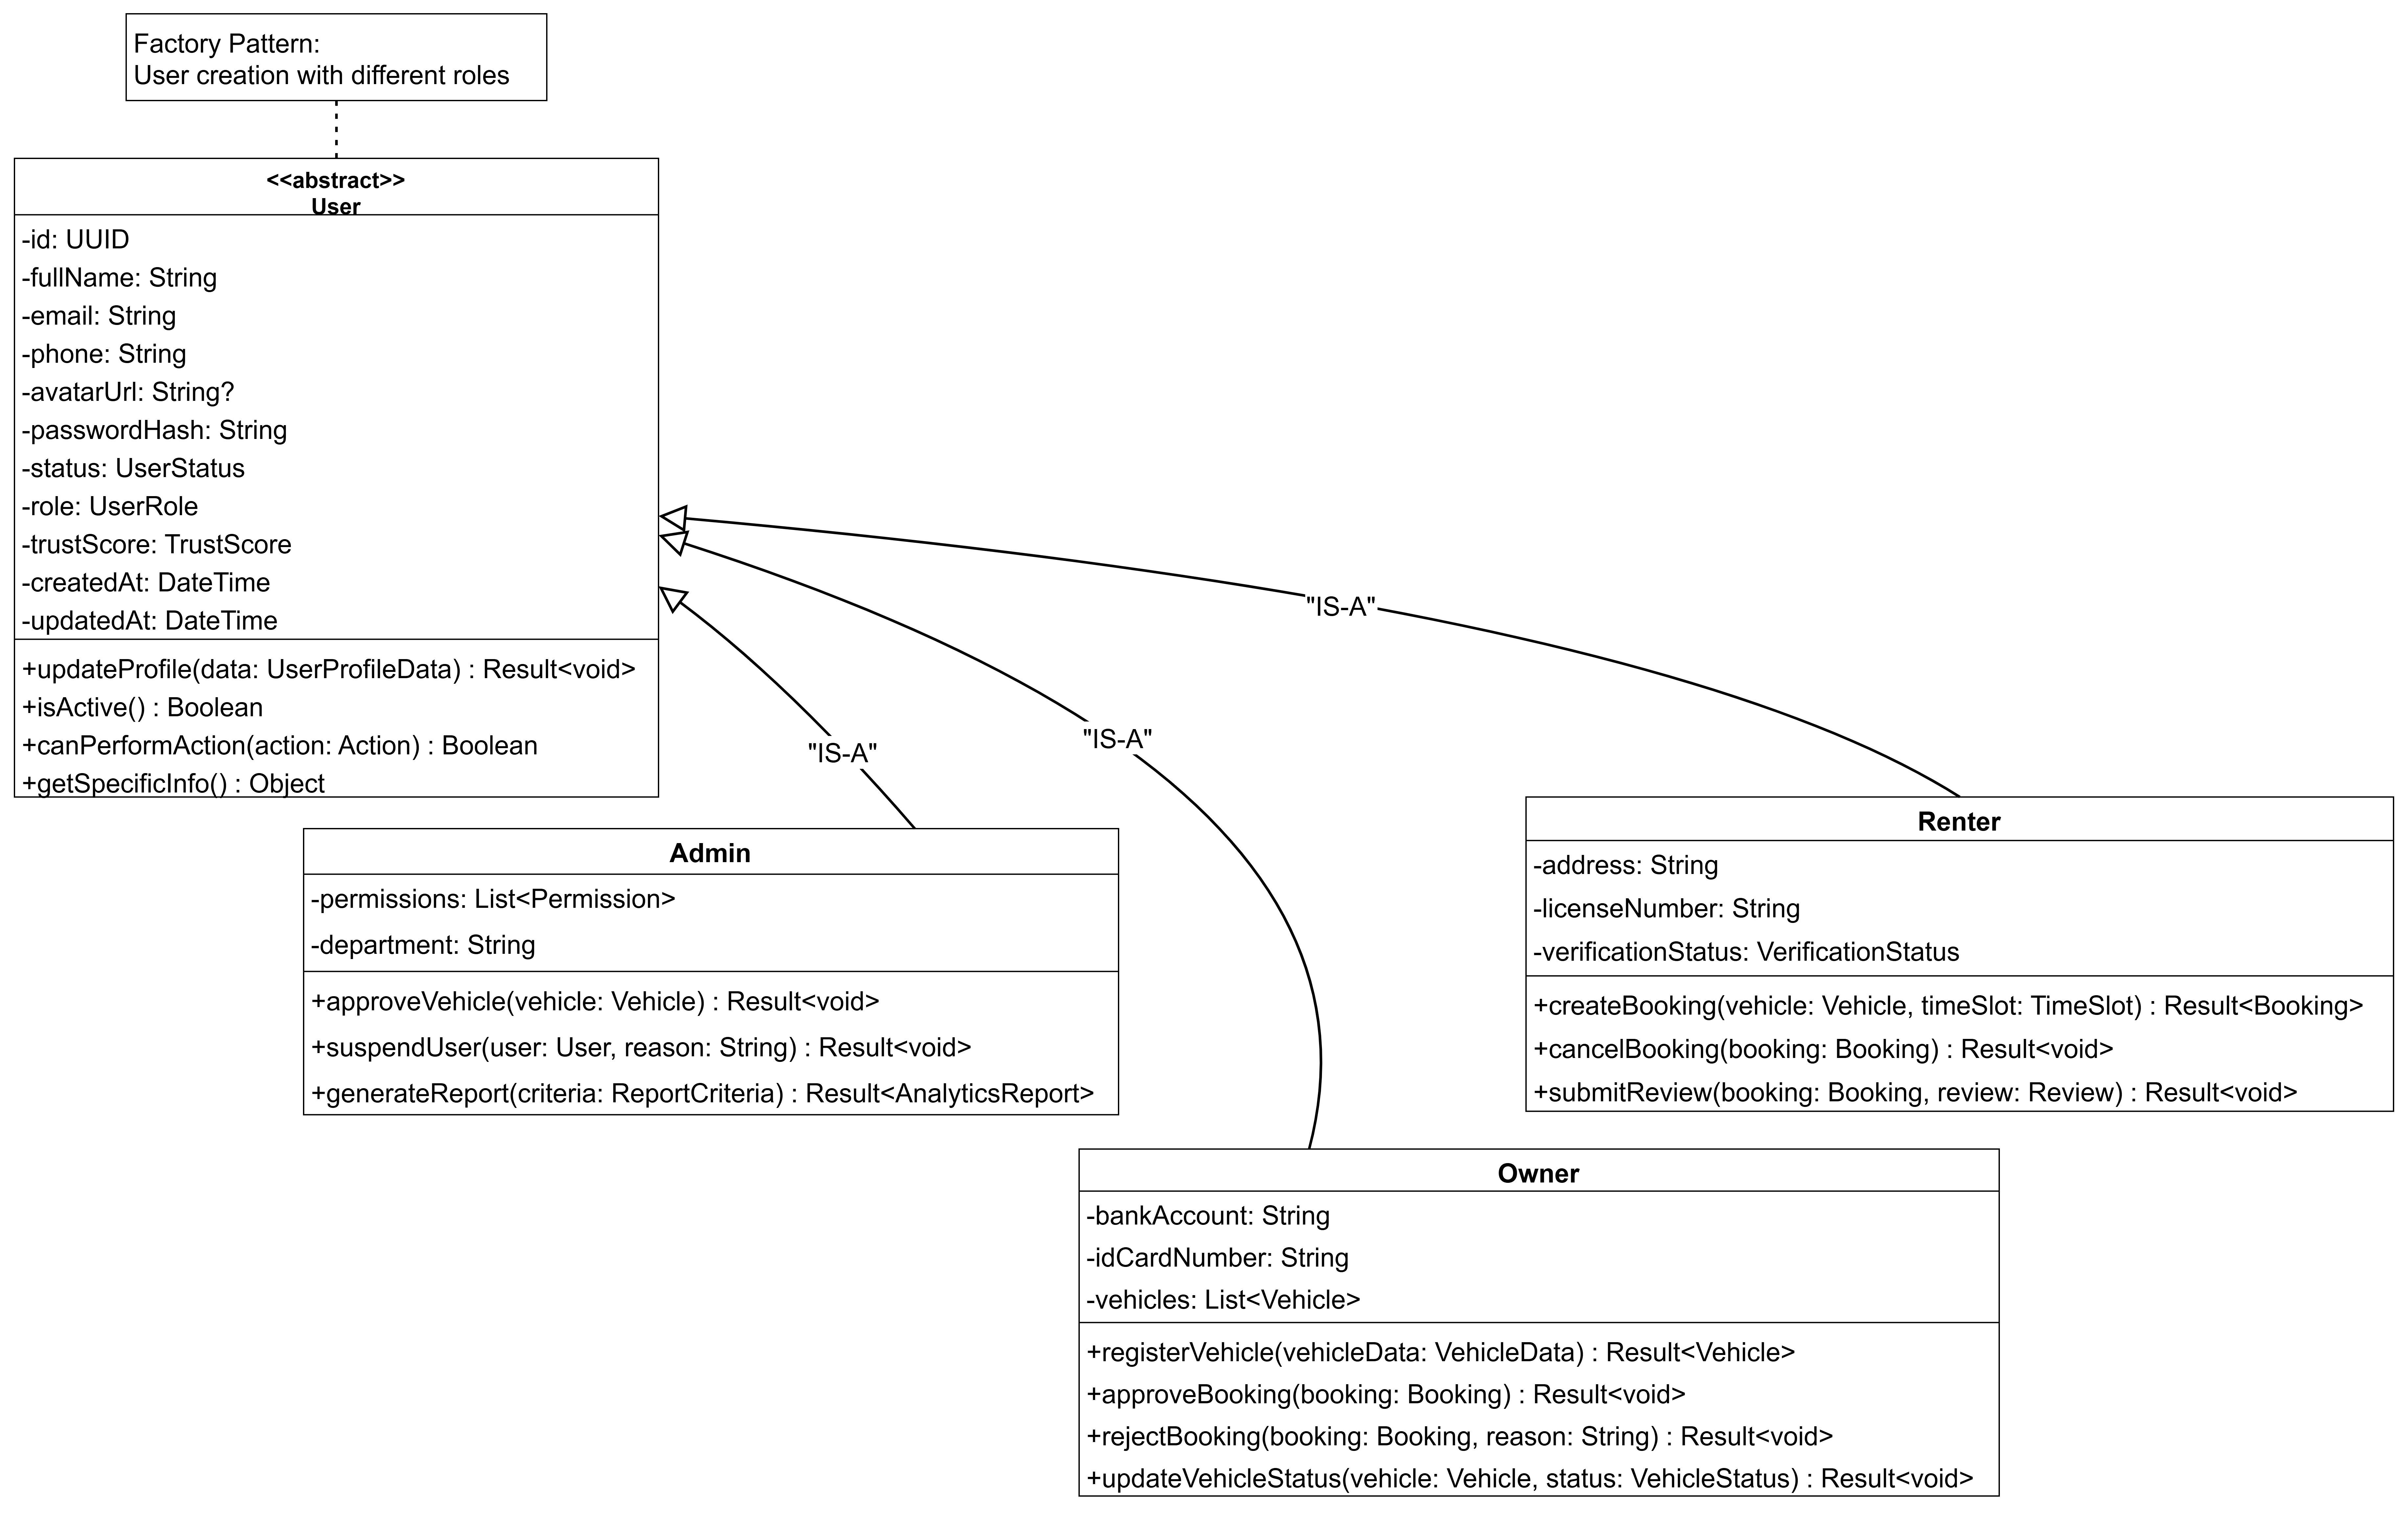
\includegraphics[width=1.0\textwidth]{Images/Class/Inheritance.png}
    \caption{ User là abstract class và các Inheritances}
    \label{fig:Inheritance-class-diagram}
\end{figure}

\begin{itemize}
    \item \textbf{Mô hình phân cấp}: User là abstract class, các role cụ thể kế thừa từ User.
    \item \textbf{Đa hình}: Mỗi role có phương thức \texttt{getSpecificInfo()} riêng.
    \item \textbf{Design Pattern}: Áp dụng \textbf{Factory Pattern} để tạo các loại User.
    \begin{itemize}
        \item {Ưu điểm}: Dễ mở rộng, tuân thủ nguyên lý Open/Closed.
        \item {Triển khai}: Ẩn logic tạo đối tượng phức tạp.
    \end{itemize}
\end{itemize}

\subsubsection{Quan Hệ Hợp Thành (Composition)}

\begin{align*}
\text{User} &\xrightarrow{\text{*--}} \text{TrustScore} \\
\text{Vehicle} &\xrightarrow{\text{*--}} \text{Location} \\
\text{Booking} &\xrightarrow{\text{*--}} \text{TimeSlot} \\
\text{Booking} &\xrightarrow{\text{*--}} \text{Location}_{\text{start}} \\
\text{Booking} &\xrightarrow{\text{*--}} \text{Location}_{\text{end}}
\end{align*}

\begin{itemize}
    \item \textbf{Đặc điểm}:
    \begin{itemize}
        \item Quan hệ ``part-of'' mạnh.
        \item Lifecycle của phần tử phụ thuộc vào đối tượng chính.
        \item Khi đối tượng chính bị hủy → phần tử con cũng bị hủy.
    \end{itemize}

    \item \textbf{Ví dụ}:
    \begin{itemize}
        \item \texttt{User} sở hữu \texttt{TrustScore} (không tồn tại độc lập).
        \item \texttt{Vehicle} có \texttt{Location}.
        \item \texttt{Booking} có \texttt{TimeSlot}.
    \end{itemize}
\end{itemize}

\begin{figure}[h]
    \centering
    \includegraphics[width=0.95\textwidth]{Images/Class/Composition.png}
    \caption{Quan hệ Composition giữa các đối tượng}
    \label{fig:Composition-class-diagram}
\end{figure}


\subsubsection{Quan Hệ Liên Kết (Association)}
\begin{align*}
\text{Owner (1)} &\rightarrow \text{Vehicle (0..*)} \\
\text{Renter (1)} &\rightarrow \text{Booking (0..*)} \\
\text{Vehicle (1)} &\rightarrow \text{Booking (0..*)} \\
\text{Booking (1)} &\rightarrow \text{Payment (0..*)} \\
\text{Booking (1)} &\rightarrow \text{Review (0..1)} \\
\text{User (1)} &\rightarrow \text{Notification (0..*)}
\end{align*}

\begin{figure}[h]
    \centering
    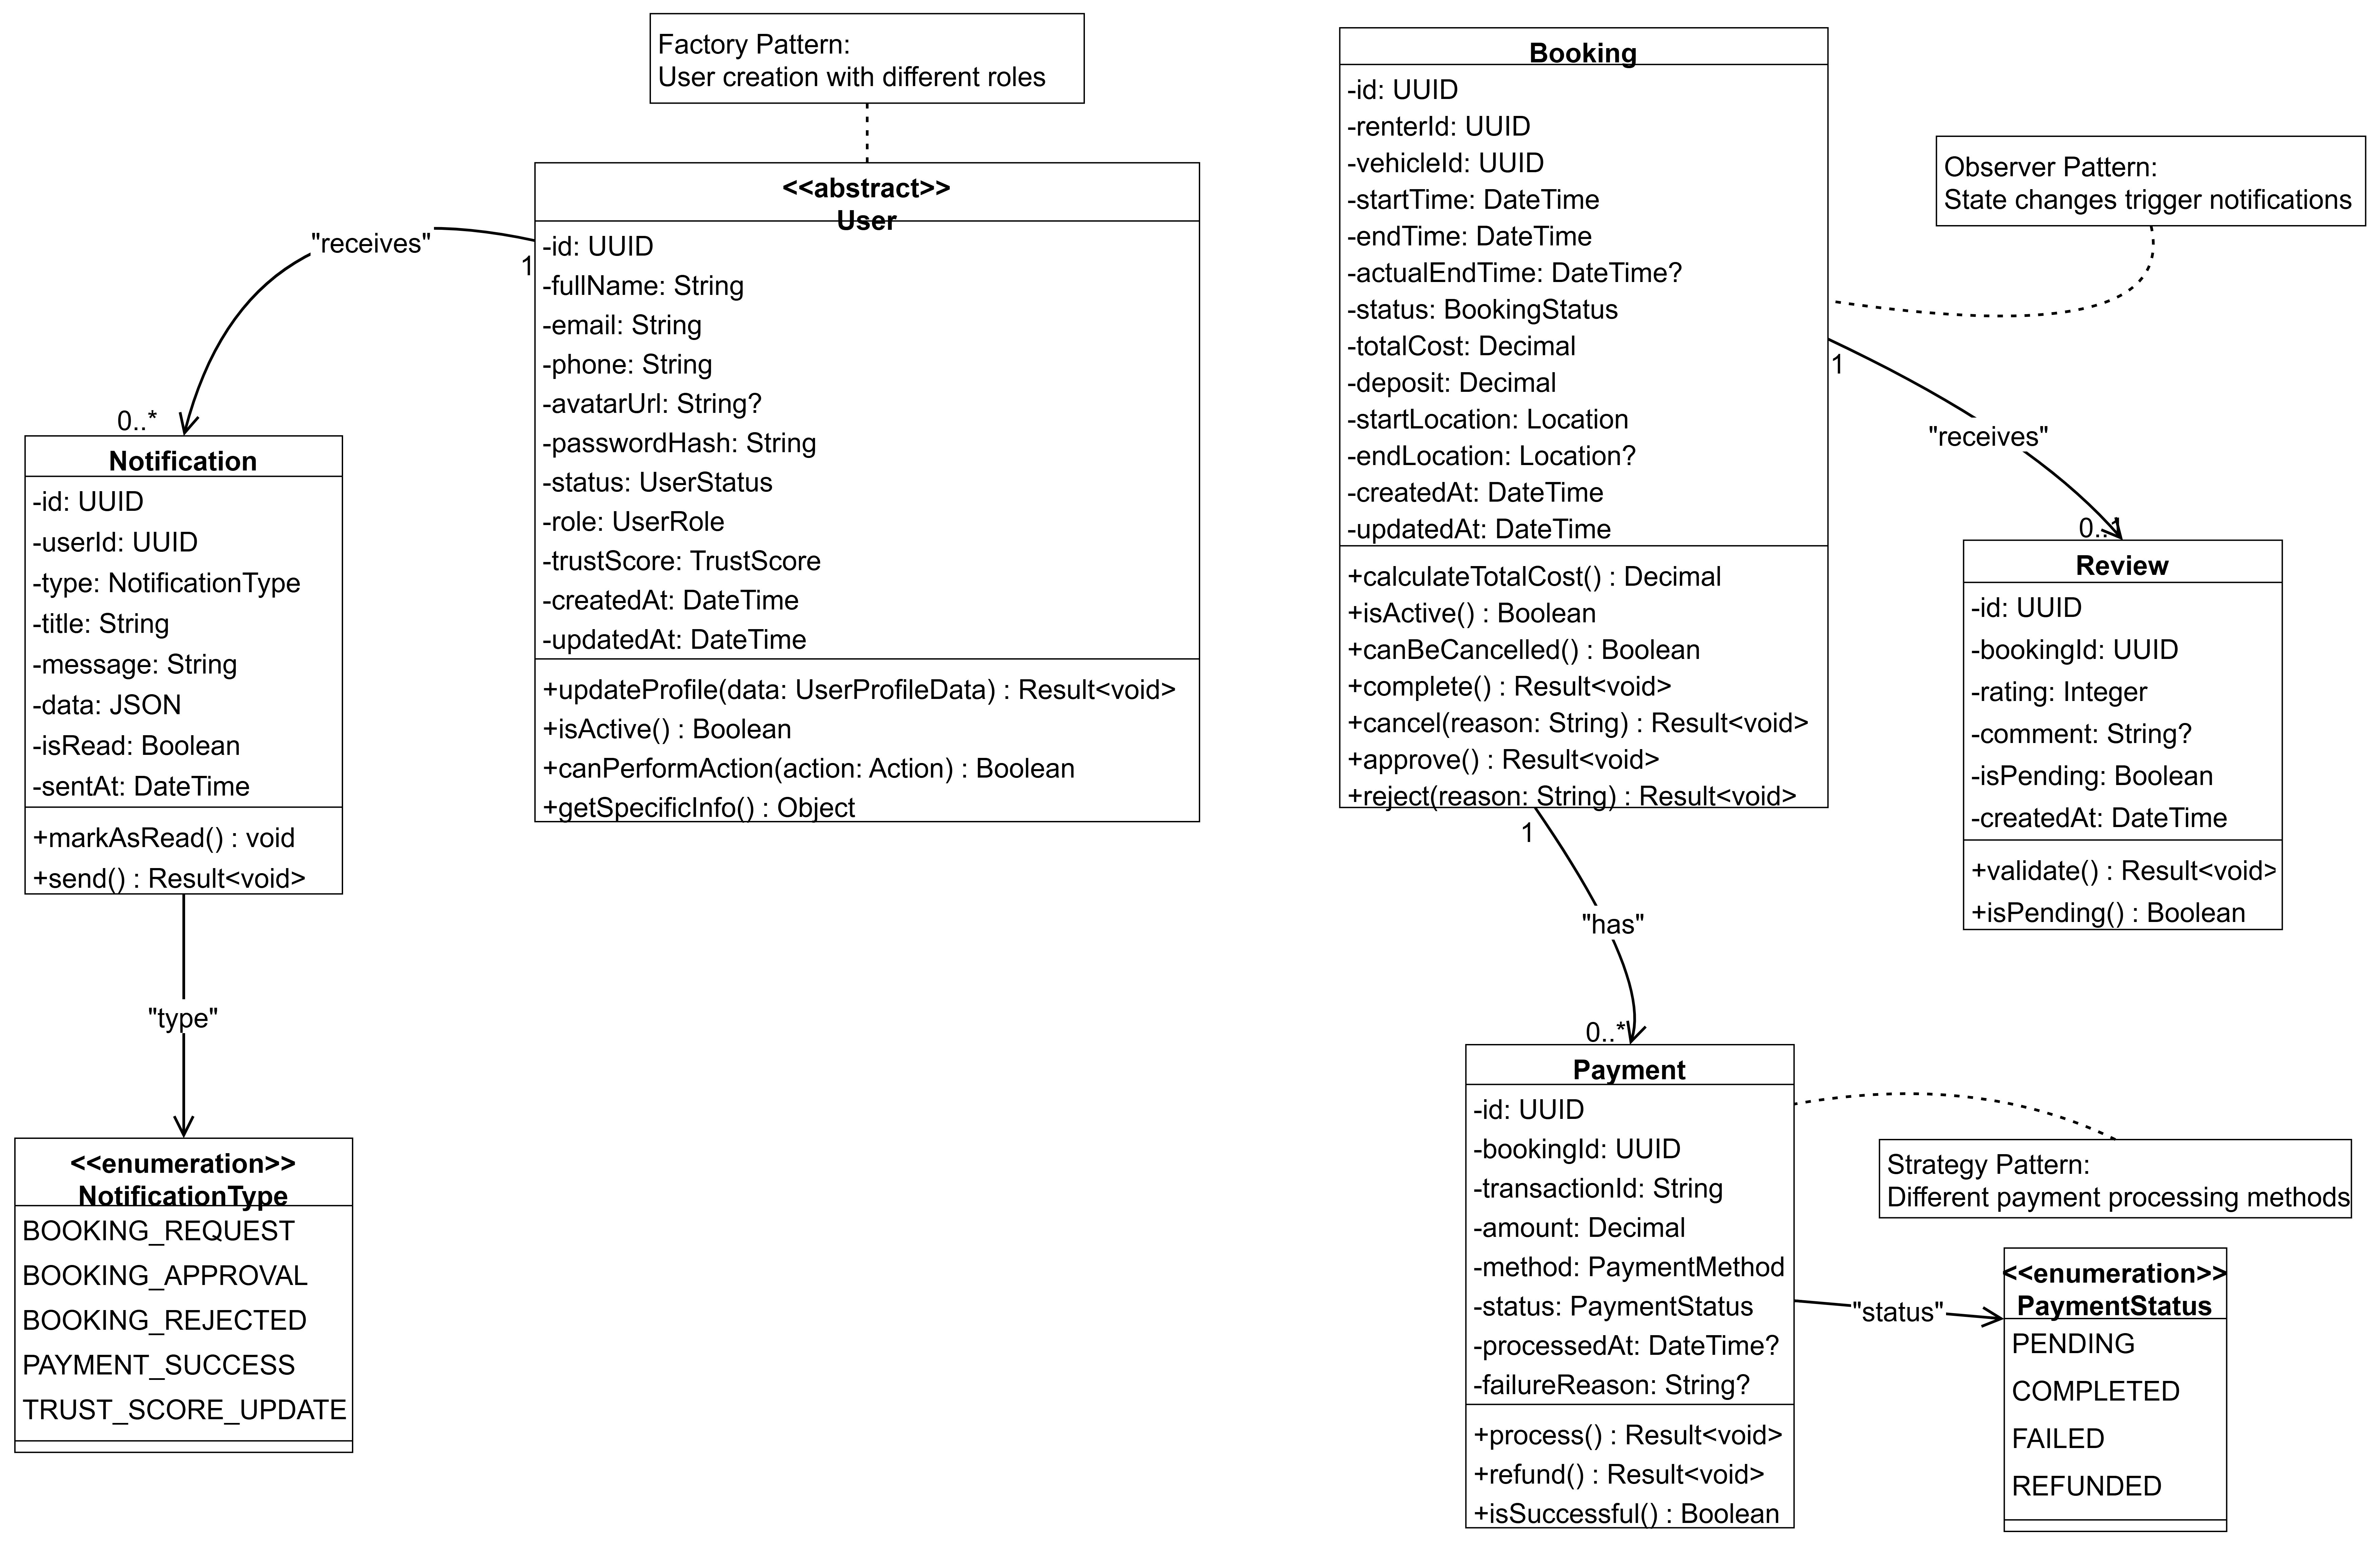
\includegraphics[width=0.95\textwidth]{Images/Class/Association.png}
    \caption{Quan hệ Association giữa các đối tượng}
    \label{fig:Association-class-diagram}
\end{figure}

\begin{itemize}
    \item \textbf{Đặc điểm}:
    \begin{itemize}
        \item Các đối tượng tồn tại độc lập.
        \item Mỗi đối tượng có lifecycle riêng.
        \item Cardinality rõ ràng.
    \end{itemize}

    \item \textbf{Ví dụ}:
    \begin{itemize}
        \item \texttt{Owner → Vehicle}: Chủ có nhiều xe.
        \item \texttt{Vehicle → Booking}: Xe được thuê nhiều lần.
        \item \texttt{Booking → Payment}: Thanh toán liên quan booking nhưng tồn tại riêng.
    \end{itemize}
\end{itemize}

\subsubsection{Quan Hệ Phụ Thuộc (Dependency)}

\begin{itemize}
    \item \textbf{Booking → Payment}:
    \begin{itemize}
        \item Booking phụ thuộc Payment để xử lý giao dịch.
        \item Áp dụng \textbf{Strategy Pattern} cho thanh toán.
    \end{itemize}

    \item \textbf{Review → Booking}:
    \begin{itemize}
        \item Review cần thông tin booking để verify.
    \end{itemize}

    \item \textbf{Notification → User}:
    \begin{itemize}
        \item Notification phụ thuộc vào User để gửi và hiển thị.
        \item Áp dụng \textbf{Command Pattern}.
    \end{itemize}
\end{itemize}

\subsubsection{Các Design Patterns Được Áp Dụng}

\subsubsection*{a. Factory Pattern}

\begin{align*}
\text{UserFactory}: \text{Role} &\rightarrow \text{User} \\
f(\text{RENTER}) &\mapsto \text{Renter instance} \\
f(\text{OWNER}) &\mapsto \text{Owner instance} \\
f(\text{ADMIN}) &\mapsto \text{Admin instance}
\end{align*}

\begin{itemize}
    \item \textbf{Mục đích}: Khởi tạo User theo role.
    \item \textbf{Lợi ích}: Open/Closed, dễ mở rộng, tái sử dụng code.
\end{itemize}

\subsubsection*{b. Observer Pattern}

\begin{equation*}
\text{Booking (Subject)} \xrightarrow{\text{notify}} 
\{\text{Renter}, \text{Owner}, \text{NotificationSystem}\}
\end{equation*}

\begin{itemize}
    \item Giảm coupling giữa các components.
    \item Dễ bổ sung observer mới.
\end{itemize}

\subsubsection*{c. Strategy Pattern}

\begin{align*}
\text{PaymentStrategy} &\supset \{\text{CreditCard}, \text{EWallet}, \text{BankTransfer}\} \\
\text{Payment} &\xrightarrow{\text{uses}} \text{PaymentStrategy}
\end{align*}

\begin{itemize}
    \item Hỗ trợ nhiều phương thức thanh toán.
    \item Tách biệt thuật toán xử lý.
\end{itemize}

\subsubsection*{d. Specification Pattern}

\begin{equation*}
\text{VehicleAvailabilitySpec} = 
f(\text{TimeSlot}) \land g(\text{Location}) \land h(\text{Battery}) \land i(\text{Status})
\end{equation*}

\begin{itemize}
    \item Kết hợp nhiều điều kiện một cách linh hoạt.
    \item Tái sử dụng logic rule.
\end{itemize}

\subsubsection*{e. Command Pattern}

\begin{equation*}
\text{Notification} \xrightarrow{\text{encapsulates}}
\{\text{SendEmail}, \text{SendSMS}, \text{PushNotification}\}
\end{equation*}

\begin{itemize}
    \item Hỗ trợ log, queue, undo.
\end{itemize}

% \subsection{Luồng Nghiệp Vụ Chính}

% \begin{align*}
% \text{Đăng ký xe} &: \text{Owner} \rightarrow \text{Vehicle} \\
% \text{Tạo booking} &: \text{Renter} \rightarrow \text{Booking} \\
% \text{Phê duyệt} &: \text{Owner} \rightarrow \text{Booking} \rightarrow \text{Notify} \\
% \text{Thanh toán} &: \text{Payment} \rightarrow \text{PaymentStrategy} \\
% \text{Hoàn tất} &: \text{Review} \rightarrow \text{TrustScore} \\
% \text{Thông báo} &: \text{Notification} \rightarrow \text{User}
% \end{align*}


\newpage
\section{Thiết kế hệ thống}
% \subsection{Kiến trúc hệ thống}
% \subsubsection{Đặc trưng của hệ thống}

% Hệ thống có những \textbf{đặc điểm kỹ thuật và nghiệp vụ} sau đây, ảnh hưởng trực tiếp đến việc chọn kiến trúc:

% \begin{longtable}{|>{\raggedright\arraybackslash}p{5cm}|>{\raggedright\arraybackslash}p{10cm}|}
% \hline
% \textbf{Nhóm đặc trưng} & \textbf{Mô tả chi tiết} \\
% \hline
% \endfirsthead

% \hline
% \textbf{Nhóm đặc trưng} & \textbf{Mô tả chi tiết} \\
% \hline
% \endhead

% \hline
% \endfoot

% 1. Nhiều loại người dùng & Hệ thống phục vụ 3 vai trò: người thuê, người chia sẻ (chủ xe), và admin. Cả 2 vai trò chính (renter/owner) đều có thể là cùng 1 người dùng. \\
% \hline
% 2. Giao tiếp thời gian thực nhẹ & Ứng dụng cần cập nhật \textbf{vị trí xe}, \textbf{tình trạng pin}, và \textbf{trạng thái thuê xe} theo thời gian gần thực (real-time-ish) nhưng không yêu cầu tốc độ quá cao như game hay trading. \\
% \hline
% 3. Dữ liệu không đồng bộ & Xe có thể được thêm, xóa, cập nhật vị trí, trạng thái thuê... thường xuyên. \\
% \hline
% 4. Hỗ trợ di động và web & Người dùng có thể thao tác qua \textbf{ứng dụng di động} (React Native) hoặc \textbf{trang web} (React.js). \\
% \hline
% 5. Khối lượng truy cập phân tán, có thể tăng dần & Hệ thống hướng đến cộng đồng dân cư / trường học, sau đó có thể mở rộng ra quy mô thành phố. Cần dễ mở rộng (scalable). \\
% \hline
% 6. Có mô-đun AI tích hợp & Module dự đoán thời gian thuê hiệu quả (ML) chạy độc lập hoặc song song với backend chính. \\
% \hline
% 7. Có yếu tố học thuật P2P & Mô phỏng cơ chế chia sẻ ngang hàng: người dùng vừa thuê vừa cho thuê, có cơ chế đánh giá uy tín (trust score). \\
% \hline
% 8. Cần bảo mật và xác thực & Dữ liệu người dùng, vị trí và giao dịch phải được bảo vệ bằng cơ chế xác thực và mã hóa. \\
% \hline
% 9. Tính mở rộng công nghệ & Dễ tích hợp thêm IoT (nếu gắn cảm biến pin xe), thanh toán điện tử, hoặc AI nâng cao sau này. \\
% \hline
% \end{longtable}

% \subsubsection*{Phân tích yêu cầu kỹ thuật (non-functional requirements)}

% \begin{longtable}{|>{\raggedright\arraybackslash}p{4cm}|>{\raggedright\arraybackslash}p{4cm}|>{\raggedright\arraybackslash}p{7cm}|}
% \hline
% \textbf{Tiêu chí} & \textbf{Mức yêu cầu} & \textbf{Ý nghĩa} \\
% \hline
% \endfirsthead

% \hline
% \textbf{Tiêu chí} & \textbf{Mức yêu cầu} & \textbf{Ý nghĩa} \\
% \hline
% \endhead

% \hline
% \endfoot

% Hiệu năng & Trung bình → Cao & Phản hồi trong $\leq$ 2s cho các thao tác chính (tìm xe, thuê xe). \\
% \hline
% Scalability (mở rộng) & Quan trọng & Có thể mở rộng khi số người thuê tăng nhanh. \\
% \hline
% Availability (sẵn sàng) & Trung bình & Không yêu cầu 24/7 nhưng phải ổn định khi sử dụng. \\
% \hline
% Maintainability (dễ bảo trì) & Cao & Kiến trúc module tách biệt, dễ nâng cấp. \\
% \hline
% Security (bảo mật) & Quan trọng & Xác thực người dùng, mã hóa JWT, ẩn vị trí chính xác của chủ xe. \\
% \hline
% Interoperability (tích hợp) & Quan trọng & Dễ tích hợp AI module, API bản đồ, thanh toán. \\
% \hline
% \end{longtable}

% \subsubsection{Các Architectural Styles phổ biến}
% \begin{longtable}{|>{\raggedright\arraybackslash}p{3cm}|>{\raggedright\arraybackslash}p{4cm}|>{\raggedright\arraybackslash}p{3.5cm}|>{\raggedright\arraybackslash}p{3.5cm}|}
% \hline
% \textbf{Style} & \textbf{Mô tả} & \textbf{Ưu điểm} & \textbf{Nhược điểm} \\
% \hline
% \endfirsthead
% \hline
% \textbf{Style} & \textbf{Mô tả} & \textbf{Ưu điểm} & \textbf{Nhược điểm} \\
% \hline
% \endhead
% \hline
% \endfoot
% Layered & Chia thành các tầng: Presentation, Application, Domain, Infrastructure. Mỗi tầng chỉ giao tiếp với tầng liền kề. & Dễ bảo trì và mở rộng. \newline Thay đổi một tầng không ảnh hưởng tầng khác. & Phức tạp khi có nhiều tầng. \newline Dễ rò rỉ logic giữa các tầng. \\
% \hline
% Monolithic & Toàn bộ ứng dụng (UI, logic, DB) trong một package duy nhất. & Đơn giản, dễ phát triển và deploy. \newline Phù hợp dự án nhỏ/MVP. & Khó scale. \newline Deploy một phần phải restart toàn bộ. \newline Logic chồng chéo. \\
% \hline
% Microservices & Chia ứng dụng thành các service độc lập, giao tiếp qua API/message queue. & Scale riêng từng service. \newline Chịu lỗi tốt. \newline Hỗ trợ CI/CD. & Hạ tầng phức tạp (Gateway, orchestration). \newline Debug khó. \newline Chi phí cao. \\
% \hline
% Event-driven & Các module giao tiếp qua sự kiện (event bus/pub-sub). & Tốt cho real-time và async. \newline Dễ mở rộng module mới. & Thiết kế phức tạp. \newline Cần message broker (Kafka, RabbitMQ). \\
% \hline
% Microkernel (Plugin) & Core system nhỏ + các plugin mở rộng chức năng. & Dễ thêm module mới. \newline Core gọn, dễ bảo trì. & Quản lý interface phức tạp. \newline Ít framework hỗ trợ. \\
% \hline
% Serverless / FaaS & Chạy các hàm độc lập trên cloud (AWS Lambda, Firebase Functions). & Không quản lý server. \newline Tự động scale. & Quản lý state khó. \newline Cold start delay. \newline Chi phí cao khi scale lớn. \\
% \hline
% \end{longtable}

% \subsubsection*{Tổng kết mức độ phù hợp với hệ thống chia sẻ xe máy điện P2P}
% \begin{longtable}{|>{\raggedright\arraybackslash}p{2.5cm}|>{\centering\arraybackslash}p{2.2cm}|>{\raggedright\arraybackslash}p{9.5cm}|}
% \hline
% \textbf{Style} & \textbf{Mức độ} & \textbf{Vai trò / Lý do} \\
% \hline
% \endfirsthead

% \hline
% \textbf{Style} & \textbf{Mức độ} & \textbf{Vai trò / Lý do} \\
% \hline
% \endhead

% \hline
% \endfoot
% Layered & \textbf{Rất cao} ⭐⭐⭐⭐☆ & \textbf{Style chính} cho toàn hệ thống. Nhiều module (user, xe, AI, P2P) cần tách tầng rõ ràng để dễ quản lý, bảo trì và mở rộng. \\
% \hline

% Event-driven & \textbf{Cao} ⭐⭐⭐☆☆ & \textbf{Cơ chế giao tiếp bổ sung}. Phù hợp real-time (vị trí xe, trạng thái thuê), AI training (học từ event), P2P sync, notification. \\
% \hline

% Microkernel & Trung bình ⭐⭐☆☆☆ & Ý tưởng plugin (AI, Payment) tốt cho \textbf{mở rộng module} sau này, nhưng không cần triển khai riêng trong đồ án. \\
% \hline

% Microservices & Trung bình ⭐⭐☆☆☆ & Ý tưởng tách module (P2P, AI, Payment) phù hợp, nhưng \textbf{setup phức tạp}, quá nặng cho quy mô đồ án. Có thể mô phỏng bằng Clean Architecture. \\
% \hline

% Monolithic & Thấp ⭐☆☆☆☆ & \textbf{Không phù hợp}. Hệ thống cần mở rộng nhiều module (AI, P2P, payment) nên kiến trúc nguyên khối sẽ cồng kềnh, khó bảo trì. \\
% \hline

% Serverless & Thấp ⭐☆☆☆☆ & Chỉ phù hợp \textbf{tác vụ nhỏ lẻ} (AI inference, notification). Toàn hệ thống cần quản lý state (rental, payment, peer state) nên không nên dùng serverless. \\
% \hline
% \end{longtable}

% \subsubsection{Layered Architecture}
% Tuy nhiên trong phạm vi Layered Architecture, có nhiều pattern triển khai như 3-Tier, MVC, hay Clean Architecture. Để đánh giá kiến trúc phù hợp nhất với đề tài, cần có so sánh chi tiết giữa các Architecture pattern này.

% % \begin{longtable}{|>{\raggedright\arraybackslash}p{3cm}|>{\raggedright\arraybackslash}p{4cm}|>{\raggedright\arraybackslash}p{4cm}|>{\raggedright\arraybackslash}p{3.5cm}|}
% % \hline
% % \textbf{Tiêu chí} & \textbf{Layered Architecture} & \textbf{Clean Architecture} & \textbf{Điểm khác biệt} \\
% % \hline
% % \endfirsthead

% % \hline
% % \textbf{Tiêu chí} & \textbf{Layered Architecture} & \textbf{Clean Architecture} & \textbf{Điểm khác biệt} \\
% % \hline
% % \endhead

% % \hline
% % \endfoot

% % Mục tiêu & Tách hệ thống thành các tầng logic (UI, Business, Data) để dễ bảo trì, mở rộng. & Đảm bảo hướng phụ thuộc luôn đi từ ngoài vào trong (về phía core business). & Clean Architecture \textbf{kế thừa} Layered Architecture, nhưng \textbf{thêm nguyên tắc phụ thuộc ngược}. \\
% % \hline
% % Cách chia tầng & Theo \textbf{chức năng kỹ thuật (technical layers)}: UI → Service → Repository → DB. & Theo \textbf{miền nghiệp vụ (domain layers)}: Entities → Use Cases → Interface Adapters → Frameworks. & Clean Architecture là \textbf{phiên bản tiến hóa} của Layered, tập trung vào domain thay vì kỹ thuật. \\
% % \hline
% % Hướng phụ thuộc & Phụ thuộc \textbf{xuôi} (UI gọi xuống Service, Service gọi xuống Repository). & Phụ thuộc \textbf{ngược} (Infrastructure phụ thuộc vào Use Cases, chứ không ngược lại). & Đây là điểm khác biệt \textbf{cốt lõi nhất}. \\
% % \hline
% % Đối tượng trung tâm & Dữ liệu / logic kỹ thuật. & Domain (business rules). & Clean chuyển "tâm" của hệ thống về \textbf{use case và entity}. \\
% % \hline
% % Testability & Khó test độc lập vì các tầng kỹ thuật phụ thuộc trực tiếp vào nhau. & Dễ test unit vì core tách rời hạ tầng (framework, DB, UI). & Clean giải quyết nhược điểm của Layered. \\
% % \hline
% % \end{longtable}

% % \begin{figure}[H]
% %     \centering
% %     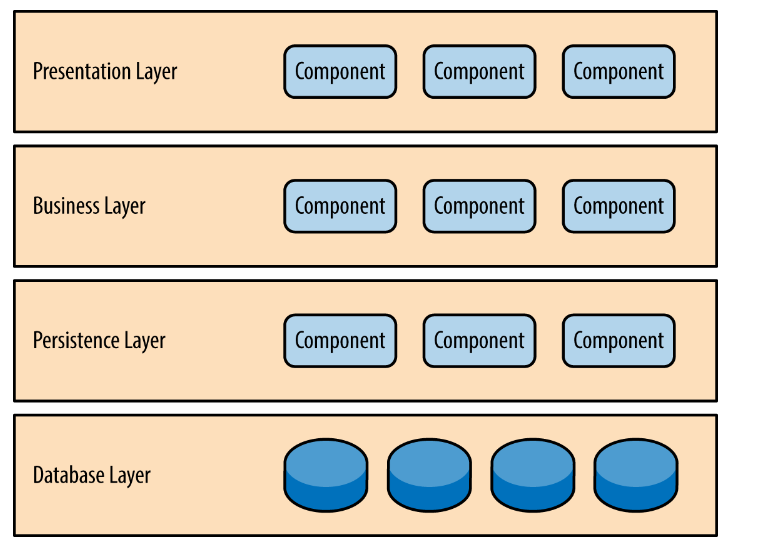
\includegraphics[width=0.7\textwidth]{Images/Arch/layer.png}
% %     \caption{Layered Architecture}
% %     \label{fig:layered-arch}
% % \end{figure}

% % \subsubsubsection*{So sánh các Architecture Pattern phổ biến trong Layer Architecture Style vs Clean Architecture}

% % \begin{longtable}{|>{\raggedright\arraybackslash}p{6.5cm}|>{\raggedright\arraybackslash}p{2.5cm}|>{\raggedright\arraybackslash}p{2.5cm}|>{\raggedright\arraybackslash}p{3cm}|}
% % \hline
% % \textbf{Tiêu chí} & \textbf{3-Tier} & \textbf{MVC} & \textbf{Clean Architecture} \\
% % \hline
% % \endfirsthead

% % \hline
% % \textbf{Tiêu chí} & \textbf{3-Tier} & \textbf{MVC} & \textbf{Clean Architecture} \\
% % \hline
% % \endhead

% % \hline
% % \endfoot

% % Tách biệt business logic khỏi infra & Trung bình & Trung bình & Cao \\
% % \hline
% % Testability & Trung bình & Trung bình & Cao \\
% % \hline
% % Dễ triển khai MVP & Cao & Cao & Trung bình \\
% % \hline
% % Tích hợp AI/externals & Trung bình & Trung bình & Cao \\
% % \hline
% % Handling real-time / event & Trung bình & Trung bình & Cao\\
% % \hline
% % \end{longtable}
% % Dựa trên những phân tích trên, hệ thống chia sẻ xe máy điện P2P sẽ sử dụng \textbf{Clean Architecture} làm kiến trúc chính, kết hợp với \textbf{Event-driven Architecture} để xử lý các tác vụ bất đồng bộ và real-time. Cụ thể:
% % \begin{itemize}
% % \item \textbf{Clean Architecture}: Cung cấp cấu trúc tổng thể cho hệ thống, đảm bảo tính module hóa, dễ bảo trì và mở rộng.
% % \item \textbf{Event-driven Architecture}: Được tích hợp như một cơ chế giao tiếp bổ sung giữa các module, đặc biệt phục vụ cho việc đồng bộ trạng thái xe, gửi thông báo real-time, và cung cấp dữ liệu cho module AI/ML.
% % \item \textbf{Client-Server}: Là nền tảng giao tiếp cơ bản giữa frontend (mobile/web) và backend thông qua RESTful API.
% % \end{itemize}

% % \begin{figure}[H]
% %     \centering
% %     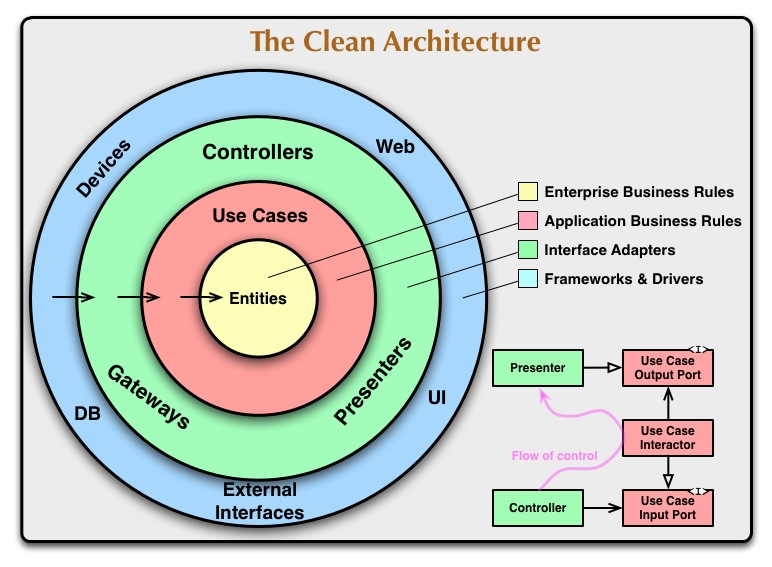
\includegraphics[width=0.7\textwidth]{Images/Arch/clean.png}
% %     \caption{Clean Architecture (Uncle Bob)}
% %     \label{fig:clean-arch}
% % \end{figure}

% \subsubsection*{a. MVC (Model -- View -- Controller)}
% Mô hình MVC được giới thiệu lần đầu bởi Trygve Reenskaug vào những năm 1970, nhằm tách biệt rõ ba phần chính trong ứng dụng: dữ liệu (Model), giao diện (View), và điều khiển (Controller).
% \begin{figure}[h]
% \centering
% 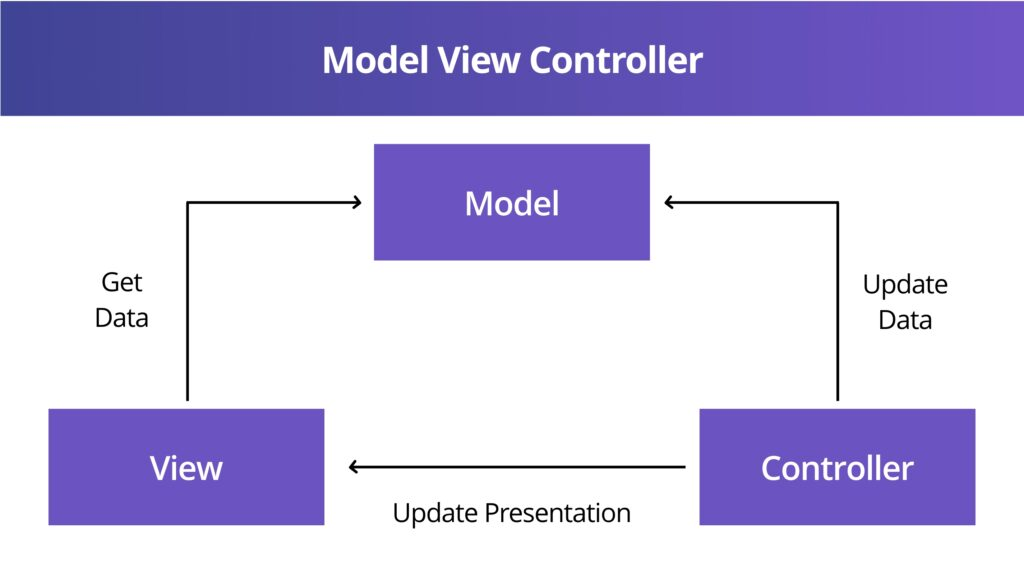
\includegraphics[height=0.3\textheight,keepaspectratio]{Images/Arch/mvc.png}
% \caption{MVC Architectural Design Pattern}
% \label{fig:mvc}
% \end{figure}

% \begin{table}[h]
% \centering
% \begin{tabular}{>{\bfseries}p{3cm}p{10cm}}
% \toprule
% \textbf{Thành phần} & \textbf{Vai trò} \\
% \midrule
% Model & Quản lý dữ liệu và logic nghiệp vụ của ứng dụng. Model nhận yêu cầu từ Controller, xử lý và trả dữ liệu lại. \\
% \addlinespace
% View & Chịu trách nhiệm hiển thị dữ liệu của Model ra giao diện, không chứa logic nghiệp vụ. \\
% \addlinespace
% Controller & Xử lý thao tác từ người dùng (user input), thực hiện xác thực (nếu cần), gọi Model để thay đổi dữ liệu, sau đó cập nhật lại View. \\
% \bottomrule
% \end{tabular}
% \end{table}
% % Người dùng tương tác với giao diện (View). Controller nhận sự kiện, gọi Model để xử lý dữ liệu. Model cập nhật dữ liệu và gửi lại kết quả cho View để hiển thị.

% \subsubsection*{Ưu điểm}
% - Tách biệt giữa dữ liệu, giao diện và điều khiển → dễ bảo trì.\\
% - Phù hợp với ứng dụng nhỏ, ít tầng logic.

% \subsubsection*{Nhược điểm}
% - Controller và View phụ thuộc chặt chẽ → thay đổi UI phải sửa Controller.\\
% - Model có thể bị truy cập trực tiếp bởi View, vi phạm nguyên tắc ``Separation of Concerns''.\\
% - Khó kiểm thử (unit test) vì Controller gắn liền với giao diện.\\



% \subsubsection*{b. MVP (Model -- View -- Presenter)}
% MVP được phát triển để khắc phục nhược điểm của MVC, bằng cách tách logic xử lý giao diện ra khỏi View, giúp dễ test và bảo trì hơn.
% \begin{figure}[h]
% \centering
% 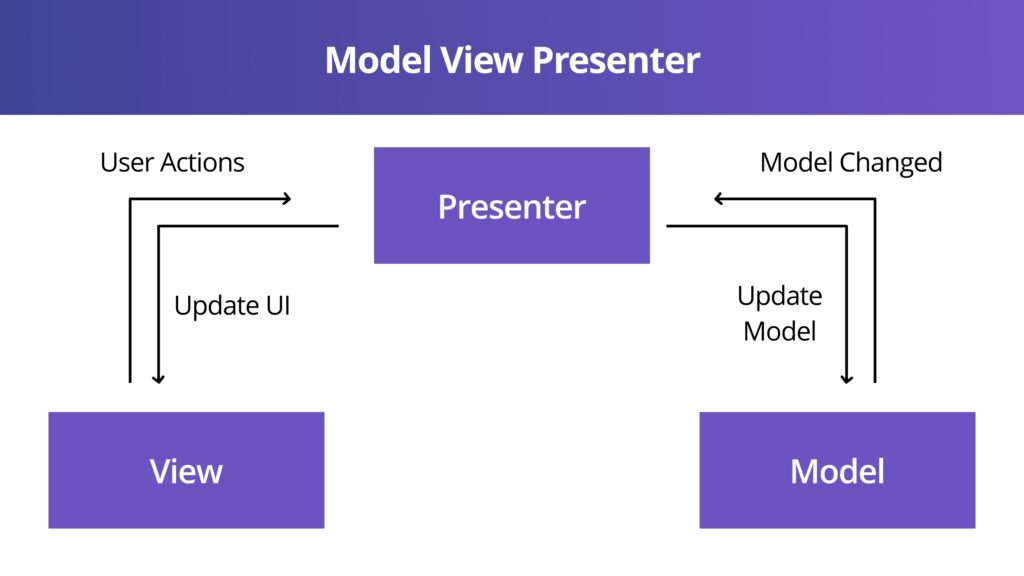
\includegraphics[height=0.3\textheight,keepaspectratio]{Images/Arch/mvp.png}
% \caption{MVP Architectural Design Pattern}
% \label{fig:mvp}
% \end{figure}

% \begin{table}[h]
% \centering
% \begin{tabular}{>{\bfseries}p{3cm}p{10cm}}
% \toprule
% \textbf{Thành phần} & \textbf{Vai trò} \\
% \midrule
% Model & Tập hợp các lớp mô tả logic nghiệp vụ và dữ liệu. Định nghĩa các quy tắc thao tác với dữ liệu. \\
% \addlinespace
% View & Hiển thị dữ liệu và chuyển tiếp sự kiện người dùng đến Presenter. Không chứa logic nghiệp vụ. \\
% \addlinespace
% Presenter & Trung gian giữa View và Model. Nhận input từ View, gọi Model xử lý, sau đó trả kết quả lại cho View để hiển thị. \\
% \bottomrule
% \end{tabular}
% \end{table}

% \subsubsection*{Ưu điểm}
% - View không biết Model tồn tại, chỉ nhận dữ liệu từ Presenter → tách biệt rõ ràng.\\
% - Dễ viết unit test cho Presenter vì không phụ thuộc vào UI framework.\\
% - Tăng khả năng tái sử dụng View và Model.

% \subsubsection*{Nhược điểm}
% - Presenter dễ trở thành ``God class'' nếu chứa quá nhiều logic.\\
% - Code nhiều hơn do phải tạo các interface giữa View $\leftrightarrow$ Presenter.\\
% - Quan hệ Presenter--View vẫn còn chặt (Presenter phải biết View để gọi update).

% \subsubsection*{c. MVVM (Model -- View -- ViewModel)}
% MVVM ra đời để loại bỏ sự phụ thuộc giữa Presenter và View trong MVP, bằng cách dùng cơ chế data binding hai chiều. Mô hình này được sử dụng phổ biến trong Android (Jetpack), iOS (SwiftUI) và Frontend (React, Vue, Angular).
% \begin{figure}[h]
% \centering
% 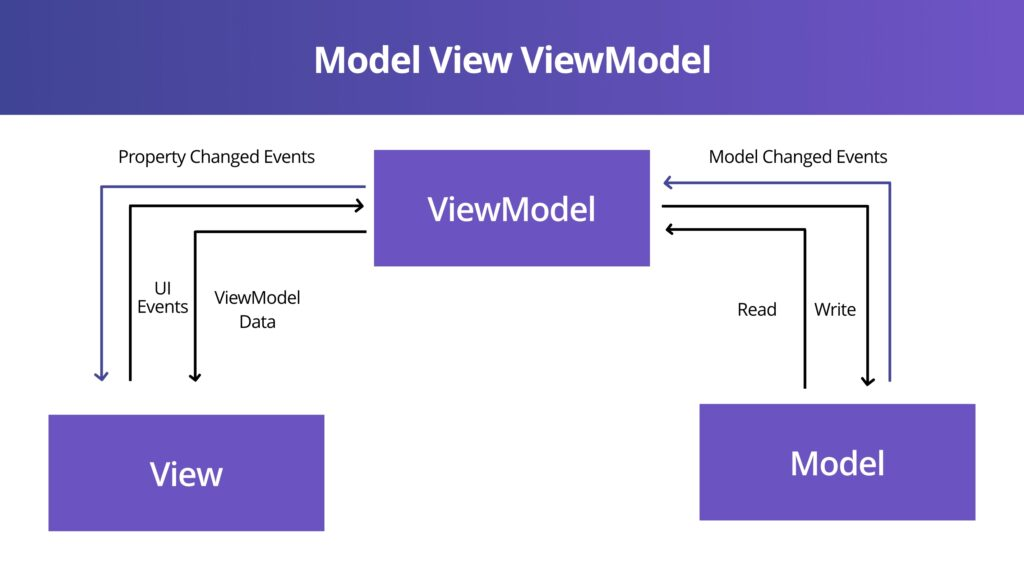
\includegraphics[height=0.3\textheight,keepaspectratio]{Images/Arch/mvvm.png}
% \caption{MVVM Architectural Design Pattern}
% \label{fig:mvvm}
% \end{figure}

% \begin{table}[h]
% \centering
% \begin{tabular}{>{\bfseries}p{3cm}p{10cm}}
% \toprule
% \textbf{Thành phần} & \textbf{Vai trò} \\
% \midrule
% Model & Lưu trữ dữ liệu và logic nghiệp vụ. Không giao tiếp trực tiếp với View. Expose dữ liệu qua các Observable/LiveData/Flow. \\
% \addlinespace
% View & Giao diện hiển thị dữ liệu, không chứa logic nghiệp vụ. Quan sát (observe) dữ liệu từ ViewModel và tự động cập nhật khi có thay đổi. \\
% \addlinespace
% ViewModel & Trung gian giữa Model và View. Gọi Model để lấy dữ liệu, xử lý và cung cấp data stream cho View. Sử dụng callback hoặc observable để cập nhật View. \\
% \bottomrule
% \end{tabular}
% \end{table}

% \subsubsection*{Ưu điểm}
% - View và ViewModel không biết nhau trực tiếp → giảm coupling.\\
% - Hỗ trợ binding tự động → code gọn, dễ bảo trì.\\
% - Dễ kiểm thử logic trong ViewModel.

% \subsubsection*{Nhược điểm}
% - Khó debug nếu có nhiều Observable phức tạp.\\
% - Dễ gây vòng lặp dữ liệu nếu binding hai chiều sai cách.\\
% - Yêu cầu hiểu biết về reactive programming.

% \subsubsection*{d. Clean Architecture}
% Clean Architecture được đề xuất bởi Robert C. Martin (Uncle Bob), nhằm chuẩn hóa cách tách biệt tầng trong ứng dụng -- đặc biệt cho các hệ thống lớn, dễ bảo trì, test và mở rộng. Kiến trúc này được chia thành các vòng (layers) đồng tâm, mọi phụ thuộc đều hướng vào trong.
% \begin{figure}[H]
%     \centering
%     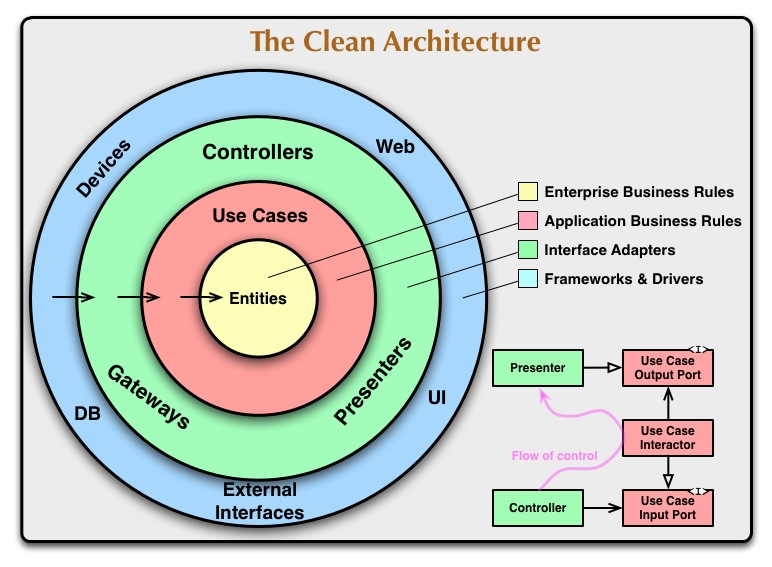
\includegraphics[width=0.9\textwidth]{Images/Arch/clean.png}
%     \caption{Clean Architecture (Uncle Bob)}
%     \label{fig:clean-arch}
% \end{figure}
% \textbf{Quy tắc phụ thuộc (Dependency Rule):} Tất cả phụ thuộc phải chỉ hướng vào trong -- nghĩa là lớp ngoài có thể gọi lớp trong, nhưng lớp trong không được biết gì về lớp ngoài.

% \newpage

% \subsubsection*{Các tầng chính}
% \begin{table}[h]
% \centering
% \begin{tabular}{>{\bfseries}p{4.5cm}p{4cm}p{4.5cm}}
% \toprule
% \textbf{Tầng} & \textbf{Thành phần chính} & \textbf{Vai trò} \\
% \midrule
% UI / Interface Layer & Controller, Presenter, ViewModel, View & Tiếp nhận và hiển thị dữ liệu với người dùng. \\
% \addlinespace
% Application Layer & UseCase Interactor, InputBoundary, OutputBoundary & Chứa logic nghiệp vụ ứng dụng (use case). \\
% \addlinespace
% Domain Layer & Entities & Chứa logic nghiệp vụ cốt lõi, không phụ thuộc framework. \\
% \addlinespace
% Infrastructure Layer & DataAccessInterface, DataAccess, Database & Thao tác lưu trữ dữ liệu (DB, API, file...). \\
% \bottomrule
% \end{tabular}
% \end{table}
% \subsubsection*{Luồng hoạt động chi tiết}
% \subsubsubsection*{Bước 1 -- Controller nhận input từ người dùng}
% \vspace{-0.3cm}
% Người dùng gửi request (qua web form, API, hay giao diện). Controller nhận dữ liệu đầu vào (Input Data) và gói lại trong một Data Transfer Object (DTO) -- ví dụ \texttt{CreateOrderRequest} hoặc \texttt{LoginRequest}. Controller không xử lý nghiệp vụ mà chuyển tiếp qua interface \texttt{InputBoundary}.
% \vspace{-0.7cm}
% \subsubsubsection*{Bước 2 -- InputBoundary chuyển dữ liệu vào Use Case}
% \vspace{-0.3cm}
% \texttt{InputBoundary} là một interface, đảm bảo Controller không phụ thuộc trực tiếp vào logic nghiệp vụ. \texttt{UseCaseInteractor} implement \texttt{InputBoundary}, nên khi Controller gọi interface này, luồng điều khiển vào bên trong Application Layer.
% \vspace{-0.5cm}
% \subsubsubsection*{Bước 3 -- Use Case Interactor thực thi nghiệp vụ}
% \vspace{-0.3cm}
% Đây là trái tim của ứng dụng (application business rules). \texttt{UseCaseInteractor}:\\
% - Gọi Entities để áp dụng logic nghiệp vụ (ví dụ: tính tổng tiền, kiểm tra điều kiện).\\
% - Dùng \texttt{DataAccessInterface} để lấy dữ liệu thật từ DB (thông qua repository).\\
% - Kết quả xử lý được đóng gói lại thành \texttt{OutputData} (cũng là POJO).
% \vspace{-0.5cm}
% \subsubsubsection*{Bước 4 -- OutputBoundary trả kết quả ra ngoài}
% \vspace{-0.3cm}
% Sau khi xử lý xong, \texttt{UseCaseInteractor} gửi \texttt{OutputData} qua \texttt{OutputBoundary} (interface). Presenter implement \texttt{OutputBoundary}, nên sẽ nhận được dữ liệu này.
% \vspace{-0.5cm}
% \subsubsubsection*{Bước 5 -- Presenter chuyển đổi dữ liệu cho UI}
% \vspace{-0.3cm}
% Presenter không xử lý nghiệp vụ mà chỉ lo định dạng dữ liệu để hiển thị:
% % \begin{itemize}[leftmargin=*]
% %     \item Chuyển Date thành chuỗi ``31/10/2025'', Currency thành ``1,000 VND''.
% %     \item Đưa các cờ (flags) như ``button enabled'', ``menu visible'' vào ViewModel.
% % \end{itemize}
% ViewModel là một Data Transfer Object (DTO) chứa dữ liệu UI-friendly.
% \vspace{-0.5cm}
% \subsubsubsection*{Bước 6 -- View hiển thị dữ liệu cho người dùng}
% \vspace{-0.3cm}
% View chỉ cần nhận ViewModel và render ra giao diện (HTML, React component, XML layout, ...). View không chứa logic nghiệp vụ, chỉ hiển thị đúng dữ liệu đã được Presenter chuẩn bị.
% \begin{figure}[h]
% \centering
% 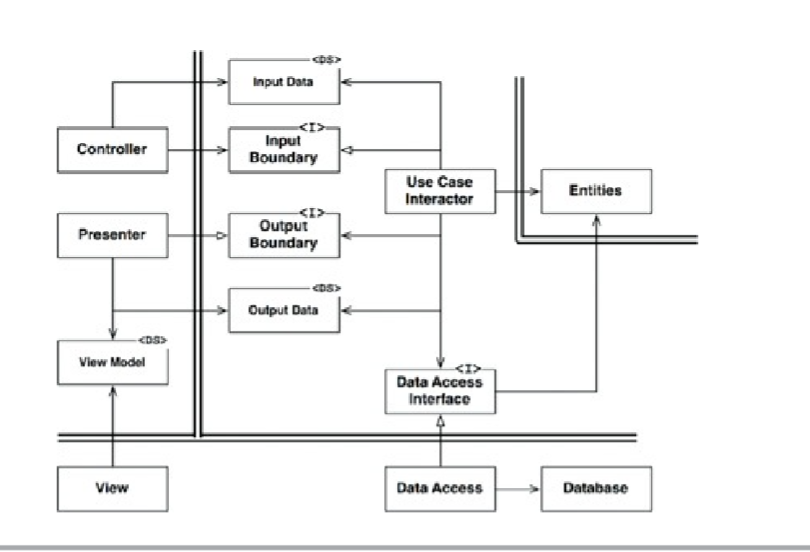
\includegraphics[height=0.5\textwidth]{Images/Arch/clean_flow.png}
% \caption{A typical scenario for a system utilizing a database follow Clean Architecture}
% \label{fig:clean_full}
% \end{figure}
% % \vspace{-0.5cm}
% % \subsubsection*{Ý nghĩa của thiết kế}
% % \begin{table}[h]
% % \centering
% % \begin{tabular}{>{\bfseries}p{5cm}p{8cm}}
% % \toprule
% % \textbf{Mục tiêu} & \textbf{Cách đạt được} \\
% % \midrule
% % Tách biệt tầng UI và logic nghiệp vụ & Qua InputBoundary, OutputBoundary và UseCaseInteractor. \\
% % \addlinespace
% % Dễ test logic nghiệp vụ & Có thể test UseCaseInteractor mà không cần DB hay UI. \\
% % \addlinespace
% % Độc lập framework & Không phụ thuộc vào Spring, Android hay bất kỳ UI lib nào. \\
% % \addlinespace
% % Thay đổi UI hoặc DB linh hoạt & Vì phụ thuộc chỉ hướng vào trong. \\
% % \bottomrule
% % \end{tabular}
% % \end{table}
% \subsubsection*{Ưu điểm}
% - Mỗi tầng chỉ phụ thuộc vào tầng ``bên trong'' → thay đổi dễ dàng.\\
% - Dễ test độc lập từng tầng.\\
% - Cho phép thay đổi framework (Android, iOS, Web) mà không động vào logic.

% \subsubsection*{Nhược điểm}
% - Cấu trúc phức tạp, nhiều lớp.\\
% - Không phù hợp cho dự án nhỏ hoặc nguyên mẫu (MVP app).

% Dựa trên những phân tích trên, hệ thống chia sẻ xe máy điện P2P sẽ sử dụng \textbf{Clean Architecture} làm kiến trúc chính, kết hợp với \textbf{Event-driven Architecture} để xử lý các tác vụ bất đồng bộ và real-time. Cụ thể:
% \begin{itemize}
% \item \textbf{Clean Architecture}: Cung cấp cấu trúc tổng thể cho hệ thống, đảm bảo tính module hóa, dễ bảo trì và mở rộng.
% \item \textbf{Event-driven Architecture}: Được tích hợp như một cơ chế giao tiếp bổ sung giữa các module, đặc biệt phục vụ cho việc đồng bộ trạng thái xe, gửi thông báo real-time, và cung cấp dữ liệu cho module AI/ML.
% \item \textbf{Client-Server}: Là nền tảng giao tiếp cơ bản giữa frontend (mobile/web) và backend thông qua RESTful API.
% \end{itemize}

\subsection{Kiến trúc hệ thống}

\subsubsection{Phân tích đặc trưng hệ thống}

Thiết kế kiến trúc của một hệ thống phần mềm phải được xây dựng trên nền tảng phân tích có hệ thống các đặc trưng kỹ thuật và nghiệp vụ \cite{bass2021}. Đối với nền tảng chia sẻ xe máy điện P2P, cần xác định một số đặc điểm phân biệt có ảnh hưởng trực tiếp đến các quyết định kiến trúc:

\textbf{Quản lý người dùng đa vai trò.} Hệ thống phục vụ ba vai trò người dùng riêng biệt: người thuê, chủ xe và quản trị viên. Đáng chú ý, người dùng cá nhân có thể hoạt động ở cả hai vai trò là người thuê và chủ xe, đòi hỏi cơ chế kiểm soát truy cập linh hoạt dựa trên vai trò. Đặc điểm này yêu cầu một kiến trúc hỗ trợ quản lý quyền động mà không ảnh hưởng đến bảo mật hoặc trải nghiệm người dùng.

\textbf{Yêu cầu giao tiếp gần thời gian thực.} Ứng dụng yêu cầu cập nhật liên tục về vị trí xe, trạng thái pin và trạng thái thuê. Mặc dù hệ thống không yêu cầu khả năng phản hồi cấp microsecond như các nền tảng giao dịch tài chính hoặc hệ thống game thời gian thực, nó phải duy trì độ tươi của dữ liệu trong giới hạn độ trễ chấp nhận được (thường là 10-30 giây cho cập nhật vị trí) để đảm bảo hiệu quả hoạt động \cite{richards2020}.

\textbf{Mẫu dữ liệu bất đồng bộ.} Tính khả dụng của xe, tọa độ vị trí, mức pin và trạng thái thuê thường xuyên thay đổi. Hệ thống phải đáp ứng các cập nhật bất đồng bộ này trong khi duy trì tính nhất quán dữ liệu trên các client phân tán. Yêu cầu này gợi ý các mẫu kiến trúc tách biệt người sản xuất dữ liệu khỏi người tiêu dùng, cho phép xử lý theo hướng sự kiện có khả năng mở rộng.

\textbf{Triển khai đa nền tảng.} Người dùng tương tác với hệ thống thông qua cả ứng dụng di động (iOS và Android) và giao diện web. Yêu cầu đa nền tảng này đòi hỏi các quyết định kiến trúc tối đa hóa khả năng tái sử dụng code giữa các nền tảng hoặc thiết lập ranh giới API rõ ràng trừu tượng hóa các triển khai cụ thể cho từng nền tảng.

\textbf{Mẫu truy cập phân tán với mở rộng dần.} Triển khai ban đầu nhắm đến các cộng đồng địa phương như khuôn viên trường đại học và khu dân cư, với khả năng mở rộng lên quy mô thành phố. Quỹ đạo tăng trưởng này yêu cầu một kiến trúc hỗ trợ mở rộng theo chiều ngang mà không cần thiết kế lại cơ bản—một đặc điểm loại bỏ một số phong cách kiến trúc nhất định khỏi danh sách xem xét \cite{newman2021}.

\textbf{Tích hợp AI/ML.} Hệ thống kết hợp các module học máy để dự đoán thời gian thuê. Các thành phần phân tích này hoạt động bán độc lập với logic giao dịch cốt lõi, gợi ý một kiến trúc module hóa đáp ứng quy trình làm việc xử lý bất đồng bộ hoặc theo lô.

\textbf{Đặc điểm P2P học thuật.} Là một dự án giáo dục minh họa các nguyên tắc chia sẻ ngang hàng, kiến trúc phải thể hiện rõ ràng các khái niệm P2P: quyền sở hữu phi tập trung, tương tác người dùng hai chiều và cơ chế tin cậy dựa trên uy tín. Yêu cầu sư phạm này ủng hộ các kiến trúc có ranh giới module rõ ràng và tách biệt các mối quan tâm một cách rõ ràng.

\textbf{Yêu cầu bắt buộc về bảo mật và xác thực.} Hệ thống xử lý dữ liệu cá nhân nhạy cảm, thông tin vị trí và giao dịch tài chính. Các quyết định kiến trúc phải ưu tiên bảo mật thông qua các lớp phòng thủ, bao gồm khả năng xác thực, ủy quyền, mã hóa dữ liệu và ghi nhật ký kiểm toán.

\subsubsection{Yêu cầu phi chức năng và trọng số}

Theo mô hình chất lượng ISO/IEC 25010 \cite{iso25010}, thiết lập các yêu cầu phi chức năng có trọng số để hướng dẫn lựa chọn kiến trúc:

\begin{table}[h]
\centering
\caption{Yêu cầu phi chức năng với trọng số ưu tiên}
\begin{tabular}{|p{4cm}|p{2.5cm}|p{7.5cm}|}
\hline
\textbf{Thuộc tính chất lượng} & \textbf{Trọng số} & \textbf{Lý do} \\
\hline
Khả năng bảo trì & Cao (0.25) & Dự án học thuật yêu cầu ranh giới module rõ ràng để phát triển lặp và tài liệu hóa. Bảo trì dài hạn bởi các thành viên nhóm khác nhau. \\
\hline
Khả năng mở rộng & Cao (0.20) & Triển khai quy mô nhỏ ban đầu phải hỗ trợ tăng trưởng lên 500+ người dùng và 100+ xe mà không cần thiết kế lại kiến trúc. \\
\hline
Khả năng kiểm thử & Cao (0.20) & Logic nghiệp vụ phức tạp (đặt xe, thanh toán, tính điểm tin cậy) yêu cầu kiểm thử đơn vị và tích hợp. Phụ thuộc rõ ràng cần thiết cho tự động hóa kiểm thử. \\
\hline
Bảo mật & Cao (0.15) & Dữ liệu cá nhân, theo dõi vị trí và thông tin thanh toán yêu cầu các biện pháp bảo mật mạnh mẽ và tuân thủ quy định bảo vệ dữ liệu. \\
\hline
Hiệu năng & Trung bình (0.10) & Thời gian phản hồi mục tiêu <2 giây cho các thao tác chính. Cập nhật thời gian thực trong khoảng 10 giây. \\
\hline
Khả năng tương tác & Trung bình (0.10) & Tích hợp với các dịch vụ bên ngoài (API bản đồ, cổng thanh toán, module AI) yêu cầu các giao diện được xác định rõ ràng. \\
\hline
\end{tabular}
\end{table}

Các yêu cầu có trọng số này cung cấp tiêu chí định lượng để đánh giá kiến trúc, đảm bảo rằng các quyết định thiết kế phù hợp với các ưu tiên của dự án thay vì sở thích chủ quan.

\subsubsection{Đánh giá các phong cách kiến trúc}

Đánh giá bốn phong cách kiến trúc nổi bật dựa trên các yêu cầu đã thiết lập bằng ma trận chấm điểm. Mỗi phong cách nhận được xếp hạng (thang điểm 1-5, trong đó 5 đại diện cho sự phù hợp tối ưu) trên các thuộc tính chất lượng chính:

\begin{table}[h]
\centering
\caption{Ma trận chấm điểm các phong cách kiến trúc.\\ \small{ (1) Monolithic, (2) Microservices, (3) Layered, (4) Event-Driven.}}
\small
\begin{tabular}{|c|c|c|c|c|c|c|c|}
\hline
\textbf{STT} & \textbf{Bảo trì} & \textbf{Mở rộng} & \textbf{Kiểm thử} & 
\textbf{Bảo mật} & \textbf{Hiệu năng} & \textbf{Tương tác} & \textbf{Điểm} \\
 & (0.25) & (0.20) & (0.20) & (0.15) & (0.10) & (0.10) & \textbf{Tổng} \\
\hline
1 & 2 & 1 & 2 & 3 & 4 & 2 & \textbf{2.15} \\
\hline
2 & 4 & 5 & 4 & 4 & 3 & 5 & \textbf{4.15} \\
\hline
3 & 5 & 3 & 4 & 4 & 3 & 4 & \textbf{4.00} \\
\hline
4 & 3 & 4 & 3 & 3 & 5 & 4 & \textbf{3.55} \\
\hline
\end{tabular}
\end{table}


\textbf{Kiến trúc Monolithic} (Điểm: 2.15). Các thiết kế monolithic truyền thống hợp nhất tất cả các thành phần ứng dụng: trình bày, logic nghiệp vụ và truy cập dữ liệu thành một đơn vị triển khai duy nhất. Mặc dù cách tiếp cận này mang lại sự đơn giản cho phát triển ban đầu và hiệu năng cao thông qua giao tiếp trong quá trình, nó thể hiện những điểm yếu nghiêm trọng về khả năng bảo trì và mở rộng \cite{newman2021}. Khi chức năng mở rộng, codebase monolithic ngày càng khó sửa đổi mà không gây ra hiệu ứng gợn sóng trên các thành phần. Hơn nữa, mở rộng yêu cầu sao chép toàn bộ ứng dụng thay vì các thành phần nghẽn cổ chai cụ thể, dẫn đến việc sử dụng tài nguyên không hiệu quả. Đối với một hệ thống dự đoán tăng trưởng module hóa (tính năng AI, tích hợp thanh toán, phân tích), phong cách monolithic thể hiện sự tích lũy nợ kỹ thuật không thể chấp nhận được.

\textbf{Kiến trúc Microservices} (Điểm: 4.15). Microservices phân tách ứng dụng thành các dịch vụ triển khai độc lập, mỗi dịch vụ đóng gói các khả năng nghiệp vụ cụ thể \cite{newman2021}. Kiến trúc này vượt trội về khả năng mở rộng các dịch vụ riêng lẻ mở rộng dựa trên nhu cầu và khả năng tương tác thông qua các API được xác định rõ ràng. Phong cách này cũng hỗ trợ sự không đồng nhất công nghệ, cho phép các dịch vụ khác nhau sử dụng các ngăn xếp công nghệ tối ưu. Tuy nhiên, microservices gây ra độ phức tạp hoạt động đáng kể: các thách thức hệ thống phân tán (độ trễ mạng, lỗi một phần), cơ chế khám phá dịch vụ, quản lý giao dịch phân tán và đường ống triển khai phức tạp \cite{richards2020}. Đối với một dự án học thuật với nhóm nhỏ (3 thành viên) và cơ sở hạ tầng DevOps hạn chế, chi phí hoạt động vượt quá lợi ích. Mặc dù đạt điểm cao nhất tổng thể, microservices đại diện cho kỹ thuật quá mức cho phạm vi dự án hiện tại.

\textbf{Kiến trúc Layered} (Điểm: 4.00). Kiến trúc phân lớp tổ chức hệ thống thành các lớp: thường là trình bày, logic ứng dụng/nghiệp vụ và truy cập dữ liệu, trong đó mỗi lớp chỉ phụ thuộc vào các lớp bên dưới nó \cite{bass2021}. Phong cách này đạt được khả năng bảo trì xuất sắc thông qua tách biệt rõ ràng các mối quan tâm: thay đổi UI không ảnh hưởng đến logic nghiệp vụ và các quy tắc nghiệp vụ vẫn độc lập với cơ chế lưu trữ dữ liệu. Mẫu này tự nhiên hỗ trợ kiểm thử thông qua tiêm phụ thuộc và hợp đồng dựa trên giao diện. Mặc dù không phân tán vốn có như microservices, các kiến trúc phân lớp đáp ứng việc mở rộng thông qua cân bằng tải trên các phiên bản được sao chép. Hạn chế chính liên quan đến chi phí hiệu năng từ việc đi qua các lớp, mặc dù điều này hiếm khi tỏ ra có vấn đề đối với các ứng dụng hướng CRUD. Kiến trúc phân lớp cung cấp sự cân bằng tối ưu giữa cấu trúc và độ phức tạp cho quy mô nhóm và yêu cầu dự án.

\textbf{Kiến trúc Event-Driven} (Điểm: 3.55). Các hệ thống hướng sự kiện giao tiếp thông qua truyền thông điệp bất đồng bộ, trong đó các thành phần xuất bản sự kiện đến một message broker và người đăng ký phản ứng tương ứng \cite{richards2020}. Phong cách này vượt trội về hiệu năng cho các tình huống thời gian thực (cập nhật vị trí xe, gửi thông báo) và hỗ trợ kết nối lỏng giữa các thành phần hệ thống. Tuy nhiên, triển khai kiến trúc hướng sự kiện yêu cầu cơ sở hạ tầng bổ sung (message broker như RabbitMQ hoặc Kafka), gây ra độ phức tạp trong việc gỡ lỗi các luồng bất đồng bộ và làm phức tạp quản lý giao dịch trên các ranh giới sự kiện. Thay vì phục vụ như phong cách kiến trúc chính, các mẫu hướng sự kiện có thể bổ sung cho kiến trúc phân lớp cho các hệ thống con cụ thể yêu cầu khả năng thời gian thực.

\subsubsection{Clean Architecture: Cách tiếp cận phân lớp tinh chỉnh}

\begin{figure}[H]
    \centering
    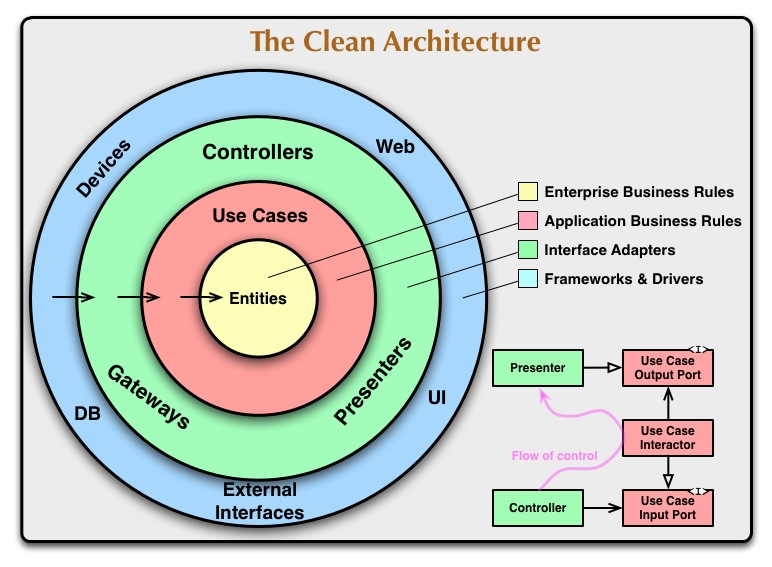
\includegraphics[width=0.85\textwidth]{Images/Arch/clean.png}
    \caption{Clean Architecture (Uncle Bob)}
    \label{fig:clean-arch}
\end{figure}

Mặc dù ma trận chấm điểm chỉ ra sự phù hợp có thể so sánh giữa kiến trúc Microservices (4.15) và Layered (4.00), các ràng buộc thực tế ủng hộ thiết kế phân lớp. Tuy nhiên, kiến trúc phân lớp truyền thống gặp phải vấn đề kết hợp chặt chẽ giữa các lớp, trong đó các lớp trên phụ thuộc trực tiếp vào các triển khai lớp dưới. Sự kết hợp này cản trở khả năng kiểm thử và làm cho việc thay thế công nghệ trở nên khó khăn \cite{martin2017}.

Clean Architecture, được đề xuất bởi Robert C. Martin, giải quyết những hạn chế này thông qua \textit{đảo ngược phụ thuộc} \cite{martin2017}. Thay vì cho phép các lớp bên ngoài phụ thuộc trực tiếp vào các triển khai bên trong, Clean Architecture yêu cầu tất cả các phụ thuộc hướng vào trong về phía logic nghiệp vụ (entities và use cases). 
Các mối quan tâm về cơ sở hạ tầng—cơ sở dữ liệu, framework, công nghệ, UI trở thành các plugin triển khai các giao diện được xác định bởi miền cốt lõi.

\subsubsection*{a. Các tầng chính}
\begin{table}[h]
\centering
\begin{tabular}{>{\bfseries}p{4.5cm}p{4cm}p{4.5cm}}
\toprule
\textbf{Tầng} & \textbf{Thành phần chính} & \textbf{Vai trò} \\
\midrule
UI / Interface Layer & Controller, Presenter, ViewModel, View & Tiếp nhận và hiển thị dữ liệu với người dùng. \\
\addlinespace
Application Layer & UseCase Interactor, InputBoundary, OutputBoundary & Chứa logic nghiệp vụ ứng dụng (use case). \\
\addlinespace
Domain Layer & Entities & Chứa logic nghiệp vụ cốt lõi, không phụ thuộc framework. \\
\addlinespace
Infrastructure Layer & DataAccessInterface, DataAccess, Database & Thao tác lưu trữ dữ liệu (DB, API, file...). \\
\bottomrule
\end{tabular}
\end{table}

\begin{figure}[h]
\centering
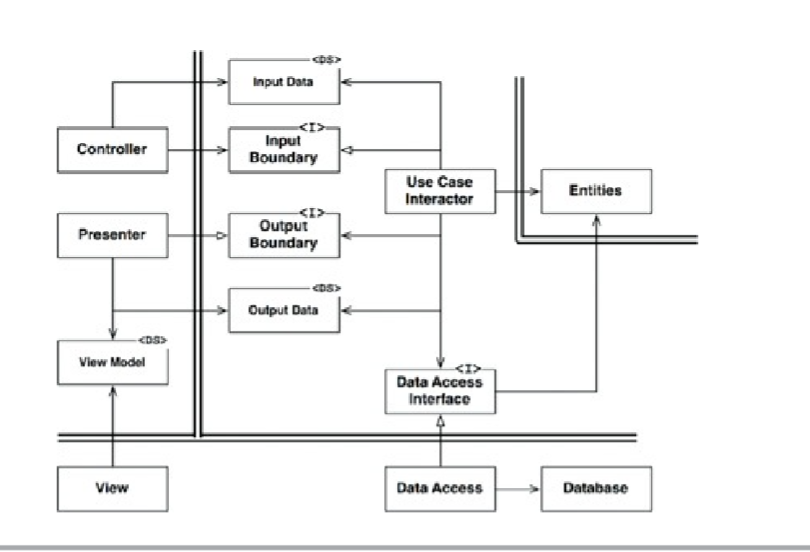
\includegraphics[height=0.5\textwidth]{Images/Arch/clean_flow.png}
\caption{A typical scenario for a system utilizing a database follow Clean Architecture}
\label{fig:clean_full}
\end{figure}

\subsubsection*{b. Luồng hoạt động chi tiết (Clean Architecture Flow)}
\textbf{Bước 1 -- Controller nhận input từ người dùng}\\
Người dùng gửi request (qua web form, API, hay giao diện). \textbf{Controller} nhận dữ liệu đầu vào (\textit{Input Data}) và gói lại trong một \textbf{Data Transfer Object (DTO)} -- ví dụ \texttt{CreateOrderRequest} hoặc \texttt{LoginRequest}. Controller không xử lý nghiệp vụ mà chuyển tiếp qua interface \texttt{InputBoundary}.
\vspace{0.3cm}

\textbf{Bước 2 -- InputBoundary chuyển dữ liệu vào Use Case}\\
\texttt{InputBoundary} là một \textbf{interface}, đảm bảo Controller không phụ thuộc trực tiếp vào logic nghiệp vụ. \texttt{UseCaseInteractor} implement \texttt{InputBoundary}, nên khi Controller gọi interface này, luồng điều khiển vào bên trong \textbf{Application Layer}.
\vspace{0.3cm}

\textbf{Bước 3 -- Use Case Interactor thực thi nghiệp vụ}\\
Đây là trái tim của ứng dụng (\textit{application business rules}). \texttt{UseCaseInteractor}:\\
-- Gọi \textbf{Entities} để áp dụng logic nghiệp vụ (ví dụ: tính tổng tiền, kiểm tra điều kiện).\\
-- Dùng \texttt{DataAccessInterface} để lấy dữ liệu thật từ DB (thông qua repository).\\
-- Kết quả xử lý được đóng gói lại thành \texttt{OutputData} (cũng là DTO).
\vspace{0.3cm}

\textbf{Bước 4 -- OutputBoundary trả kết quả ra ngoài}\\
Sau khi xử lý xong, \texttt{UseCaseInteractor} gửi \texttt{OutputData} qua \texttt{OutputBoundary} (interface). \textbf{Presenter} implement \texttt{OutputBoundary}, nên sẽ nhận được dữ liệu này.
\vspace{0.3cm}

\textbf{Bước 5 -- Presenter chuyển đổi dữ liệu cho UI}\\
Presenter không xử lý nghiệp vụ mà chỉ lo định dạng dữ liệu để hiển thị:\\
-- Chuyển Date thành chuỗi ``31/10/2025'', Currency thành ``1,000 VND''.\\
-- Đưa các cờ (flags) như ``button enabled'', ``menu visible'' vào \textbf{ViewModel}.

ViewModel là một Data Transfer Object (DTO) chứa dữ liệu UI-friendly.
\vspace{0.3cm}

\textbf{Bước 6 -- View hiển thị dữ liệu cho người dùng}\\
\textbf{View} chỉ cần nhận ViewModel và render ra giao diện (HTML, React component, XML layout, ...). View không chứa logic nghiệp vụ, chỉ hiển thị đúng dữ liệu đã được Presenter chuẩn bị.

\subsubsection*{c. Cải tiến kiến trúc này mang lại một số lợi thế phù hợp với yêu cầu dự án:}

\textbf{Khả năng kiểm thử nâng cao.} Các lớp logic nghiệp vụ hoàn toàn độc lập với cơ sở hạ tầng. Các bài kiểm thử đơn vị xác minh các use case mà không yêu cầu kết nối cơ sở dữ liệu hoặc framework UI, cải thiện đáng kể tốc độ thực thi kiểm thử và độ tin cậy.

\textbf{Độc lập công nghệ.} Miền cốt lõi xác định các hợp đồng (giao diện) thay vì phụ thuộc vào các công nghệ cụ thể. Thay thế PostgreSQL bằng MongoDB, hoặc chuyển từ NestJS sang Spring Boot, chỉ yêu cầu các triển khai adapter mới mà không sửa đổi các quy tắc nghiệp vụ.

\textbf{Không phụ thuộc framework.} Không giống như các framework MVC truyền thống kết hợp chặt chẽ code ứng dụng với các lớp framework, Clean Architecture cô lập các phụ thuộc framework tại các ranh giới hệ thống. Sự độc lập này giảm khóa nhà cung cấp và tạo điều kiện nâng cấp framework.

\textbf{Ranh giới module rõ ràng.} Kiến trúc xác định rõ ràng bốn lớp khái niệm: Entities (mô hình miền), Use Cases (quy tắc nghiệp vụ ứng dụng), Interface Adapters (controllers, presenters, gateways) và Frameworks \& Drivers (công cụ bên ngoài). Các ranh giới này phù hợp với các mẫu cộng tác nhóm, trong đó các thành viên khác nhau có thể làm việc trên các lớp khác nhau với xung đột tối thiểu.

\subsubsection{Quyết định kiến trúc}

Dựa trên đánh giá định lượng và phân tích định tính, chọn \textbf{Clean Architecture} làm phong cách kiến trúc chính, với tích hợp có chọn lọc các \textbf{mẫu Event-Driven} cho các hệ thống con thời gian thực. Quyết định này được biện minh thông qua lý do sau:

\textbf{Phù hợp với ràng buộc dự án.} Sự tách biệt lớp rõ ràng của Clean Architecture hỗ trợ cấu trúc nhóm ba người bằng cách thiết lập quyền sở hữu module rõ ràng và giảm xung đột merge. Sự nhấn mạnh của kiến trúc vào khả năng kiểm thử đáp ứng yêu cầu học thuật về chất lượng code và tài liệu có thể chứng minh \cite{martin2017}.

\textbf{Độ phức tạp cân bằng.} Trong khi microservices cung cấp khả năng mở rộng vượt trội, chúng yêu cầu chuyên môn về hệ thống phân tán và cơ sở hạ tầng DevOps vượt quá tài nguyên dự án. Clean Architecture cung cấp 80\% lợi ích về khả năng bảo trì và mở rộng với 40\% độ phức tạp triển khai, đại diện cho tỷ lệ nỗ lực-lợi ích tối ưu \cite{richards2020}.

\textbf{Giá trị giáo dục.} Kiến trúc thể hiện rõ ràng các nguyên tắc kỹ thuật phần mềm: tách biệt các mối quan tâm, đảo ngược phụ thuộc, tách biệt giao diện và trách nhiệm đơn lẻ. Những lợi ích sư phạm này phù hợp với các mục tiêu học tập của dự án học thuật.

\textbf{Đáp ứng tăng trưởng.} Mặc dù ban đầu triển khai ở quy mô nhỏ (50 xe, 150 người dùng), bản chất module hóa của Clean Architecture hỗ trợ thêm tính năng gia tăng—các công cụ khuyến nghị AI, phân tích nâng cao, tích hợp bên thứ ba—mà không cần tái cấu trúc kiến trúc. Lớp use case có thể mở rộng với các yêu cầu nghiệp vụ mới trong khi duy trì các định nghĩa entity ổn định.

\textbf{Chiến lược công nghệ.} Các mẫu hướng sự kiện bổ sung cho Clean Architecture cho các yêu cầu cụ thể: cập nhật vị trí thời gian thực (qua WebSocket), gửi thông báo (qua hàng đợi thông điệp) và thu thập dữ liệu phân tích (qua streaming sự kiện). Những mẫu chiến thuật này tích hợp như các adapter trong framework Clean Architecture thay vì quyết định cấu trúc hệ thống tổng thể.

Quyết định kiến trúc thừa nhận các đánh đổi: Clean Architecture đưa ra nhiều code boilerplate ban đầu hơn so với các framework monolithic và đảo ngược phụ thuộc yêu cầu tuân thủ kỷ luật các hợp đồng giao diện. Tuy nhiên, những chi phí này đại diện cho các khoản đầu tư trả trước mang lại lợi ích khả năng bảo trì dài hạn—một sự trao đổi đáng giá cho một hệ thống dự định chứng minh các thực hành phát triển phần mềm chuyên nghiệp.
\subsection{Lựa chọn công nghệ}

\subsubsection{Frontend}

\subsubsection*{Mục tiêu}
\begin{itemize}[leftmargin=*]
    \item Cross-platform mobile (Android/iOS)
    \item Hiển thị bản đồ, GPS, cập nhật real-time
    \item Kết nối REST API \& WebSocket
    \item Hiệu năng tốt, UI thân thiện
\end{itemize}

% \subsubsection{So sánh ngôn ngữ phổ biến}

% \begin{table}[h]
% \centering
% \begin{tabular}{>{\bfseries}p{3cm}p{5cm}p{5.5cm}}
% \toprule
% \textbf{Ngôn ngữ} & \textbf{Ưu điểm} & \textbf{Nhược điểm} \\
% \midrule
% Dart (Flutter) & Hiệu năng cao (native code). \newline UI đồng nhất, đẹp. \newline Clean Architecture tự nhiên. \newline Hot reload nhanh. & Không cùng stack với backend. \newline Không tái sử dụng code web. \newline Kích thước APK lớn. \\
% \addlinespace
% JavaScript/TypeScript (React Native) & Cùng ngôn ngữ backend. \newline Tái sử dụng logic web. \newline Cộng đồng lớn. \newline APK nhỏ hơn. & Hiệu năng thấp hơn Flutter. \newline Phụ thuộc bridge JS-Native. \newline UI ít đồng nhất. \\
% \bottomrule
% \end{tabular}
% \end{table}

\subsubsection*{Một số framework front-end phổ biến}

\begin{longtable}{|>{\raggedright\arraybackslash}p{3.5cm}|>{\raggedright\arraybackslash}p{5cm}|>{\raggedright\arraybackslash}p{5cm}|}
\hline
\textbf{Tiêu chí} & \textbf{Flutter (Dart)} & \textbf{React Native (JS/TS)} \\
\hline
\endfirsthead
\hline
\textbf{Tiêu chí} & \textbf{Flutter} & \textbf{React Native} \\
\hline
\endhead
\hline
\endfoot

Hiệu năng & \textbf{Rất cao (native code)} & Tốt (bridge JS-Native) \\
\hline
Tích hợp bản đồ & Google Maps, Mapbox plugin & react-native-maps \\
\hline
Real-time (WebSocket) & socket\_io\_client & Socket.io (cùng stack) \\
\hline
UI customization & \textbf{Rất cao, đồng nhất} & Phụ thuộc native components \\
\hline
Kích thước APK & Lớn hơn (60-80MB) & Nhỏ hơn (40-50MB) \\
\hline
Cộng đồng & Đang phát triển mạnh & Lớn, nhiều thư viện \\
\hline
Clean Architecture & \textbf{Tốt nhất (domain-data-presentation)} & Khả thi (Redux + layers) \\
\hline
Hot reload & \textbf{Rất nhanh} & Nhanh \\
\hline
Learning curve & Cao (Dart mới) & Thấp (JS phổ biến) \\
\hline
Tích hợp backend Node.js & Tốt (REST/WebSocket) & \textbf{Rất tốt (cùng JS)} \\
\hline
Tái sử dụng code web & Không (riêng Flutter Web) & \textbf{Có (React.js)} \\
\hline
\end{longtable}

% \subsubsection{Lựa chọn: Flutter}

\textbf{Lựa chọn Flutter:}
\begin{itemize}[leftmargin=*]
    \item \textbf{Hiệu năng vượt trội}: Compile ra native code, không cần bridge → mượt mà hơn, quan trọng cho ứng dụng bản đồ real-time
    \item \textbf{UI đồng nhất và đẹp}: Widget system mạnh mẽ, giao diện giống hệt trên iOS và Android
    \item \textbf{Clean Architecture tự nhiên}: Dart hỗ trợ tốt pattern domain-data-presentation, dependency injection rõ ràng
    \item \textbf{Hot reload nhanh}: Tăng tốc độ phát triển, debug dễ dàng
    \item \textbf{Phù hợp dự án học tập}: Thể hiện kỹ năng học công nghệ mới, kiến trúc rõ ràng hơn
    \item \textbf{Google hỗ trợ}: Tài liệu tốt, plugin chính thức (Maps, Location, WebSocket)
\end{itemize}

\textbf{Trade-off chấp nhận được:}
\begin{itemize}[leftmargin=*]
    \item Không cùng ngôn ngữ với backend: Vẫn giao tiếp tốt qua REST API và WebSocket, không ảnh hưởng kiến trúc Clean
    \item APK lớn hơn: Chấp nhận được với mobile hiện đại (storage đủ lớn)
    \item Learning curve: Dart dễ học, syntax giống Java/JavaScript
\end{itemize}

\subsubsection{Backend}

\subsubsection*{Mục tiêu}
\begin{itemize}[leftmargin=*]
    \item Tương thích Clean Architecture (Layered)
    \item Hỗ trợ REST API, WebSocket, database
    \item Tích hợp AI module và P2P service
    \item Dễ deploy trên cloud
    \item Dễ mở rộng module (Auth, Payment, AI)
\end{itemize}

\subsubsection*{Lựa chọn ngôn ngữ}

\begin{longtable}{|>{\raggedright\arraybackslash}p{2.5cm}|>{\raggedright\arraybackslash}p{5cm}|>{\raggedright\arraybackslash}p{5.5cm}|}
\hline
\textbf{Ngôn ngữ} & \textbf{Ưu điểm} & \textbf{Nhược điểm / Đánh giá} \\
\hline
\endfirsthead
\hline
\textbf{Ngôn ngữ} & \textbf{Ưu điểm} & \textbf{Nhược điểm / Đánh giá} \\
\hline
\endhead
\hline
\endfoot

Java & Chuẩn doanh nghiệp, DI tốt, bảo mật mạnh & Nặng, setup phức tạp. \newline \textbf{Không phù hợp đồ án.} \\
\hline
JavaScript/ TypeScript (Node.js) & Non-blocking I/O, hiệu năng cao. \newline Hỗ trợ real-time tốt (Socket.io). \newline Dễ tổ chức Clean Architecture. \newline Cùng ngôn ngữ với frontend. & Xử lý logic đồng bộ phức tạp cần cẩn thận. \newline \textbf{Rất phù hợp.} \\
\hline
Python & ORM mạnh (Django), dễ tích hợp AI & WebSocket phức tạp (Channels). \newline Cấu trúc MTV cứng nhắc. \newline \textbf{Phù hợp trung bình.} \\
\hline
\end{longtable}

\textbf{Lựa chọn: JavaScript/TypeScript (Node.js)}
\begin{itemize}[leftmargin=*]
    \item Cùng ngôn ngữ với frontend React Native → chia sẻ types, dễ debug
    \item Non-blocking I/O → phù hợp xử lý nhiều request đồng thời
    \item Hỗ trợ WebSocket tốt → phù hợp P2P và real-time
    \item Dễ gọi AI service Python qua REST API
    \item Cộng đồng lớn, dễ deploy
\end{itemize}

\subsubsection*{Các framework back-end Node.js phổ biến}

\begin{longtable}{|>{\raggedright\arraybackslash}p{2.5cm}|>{\raggedright\arraybackslash}p{5cm}|>{\raggedright\arraybackslash}p{6cm}|}
\hline
\textbf{Framework} & \textbf{Ưu điểm} & \textbf{Nhược điểm / Đánh giá} \\
\hline
\endfirsthead
\hline
\textbf{Framework} & \textbf{Ưu điểm} & \textbf{Nhược điểm / Đánh giá} \\
\hline
\endhead
\hline
\endfoot

Express.js & Nhẹ, linh hoạt, đơn giản & Không có cấu trúc sẵn, cần tự tổ chức. \newline Thiếu DI, decorator. \newline \textbf{Phù hợp dự án nhỏ.} \\
\hline
NestJS & Kiến trúc module rõ ràng. \newline DI, decorator tích hợp sẵn. \newline Hỗ trợ TypeScript tốt. \newline Template Clean Architecture có sẵn. \newline WebSocket built-in. & Phức tạp hơn Express. \newline Learning curve cao hơn. \newline \textbf{Rất phù hợp Clean Architecture.} \\
\hline
Fastify & Hiệu năng cao nhất & Cộng đồng nhỏ hơn. \newline Plugin ít hơn. \newline \textbf{Phù hợp trung bình.} \\
\hline
\end{longtable}

\textbf{Lựa chọn: NestJS}
\begin{itemize}[leftmargin=*]
    \item Hỗ trợ Clean Architecture tốt nhất (module, DI, layers)
    \item Decorator và TypeScript → code rõ ràng, dễ bảo trì
    \item WebSocket tích hợp sẵn → phù hợp P2P và real-time
    \item Template có sẵn cho Clean Architecture
    \item Dễ mở rộng module (Auth, Payment, AI)
\end{itemize}

\textbf{Ngoài ra chọn: Python (FastAPI) cho triển khai AI/ML Service sau này}
\begin{itemize}[leftmargin=*]
    \item Python là ngôn ngữ chuẩn cho ML/AI (scikit-learn, TensorFlow, PyTorch)
    \item FastAPI: hiệu năng cao, async, dễ tích hợp model
    \item Chạy độc lập như microservice, giao tiếp với backend qua REST API
    \item Không ảnh hưởng đến kiến trúc chính
\end{itemize}

\subsubsection{Database}
\subsubsection*{Mục tiêu}
\begin{itemize}[leftmargin=*]
    \item Lưu trữ dữ liệu quan hệ (users, vehicles, rentals, payments)
    \item Hỗ trợ transaction (ACID) cho payment và booking
    \item Hiệu năng tốt cho truy vấn phức tạp (join, aggregation)
    \item Khả năng mở rộng và backup dễ dàng
    \item Tích hợp tốt với NestJS (ORM)
\end{itemize}
\textbf{Lựa chọn PostgreSQL:}
\begin{itemize}[leftmargin=*]
    \item \textbf{ACID compliance}: Đảm bảo tính toàn vẹn dữ liệu cho payment và rental transactions
    \item \textbf{Spatial data support}: PostGIS extension hỗ trợ location queries (tìm xe gần, tính khoảng cách)
    \item \textbf{JSON support}: Lưu trữ metadata linh hoạt (vehicle specifications, user preferences)
    \item \textbf{TypeORM integration}: NestJS tích hợp sẵn TypeORM, hỗ trợ PostgreSQL tốt nhất
    \item \textbf{Advanced features}: Full-text search, materialized views, trigger cho event-driven
    \item \textbf{Scalability}: Replication, partitioning cho mở rộng sau này
    \item \textbf{Open-source}: Không phí license, cộng đồng lớn
\end{itemize}
% \subsubsection*{Một số cơ sở dữ liệu phổ biến}

% \begin{longtable}{|>{\raggedright\arraybackslash}p{2.5cm}|>{\raggedright\arraybackslash}p{5cm}|>{\raggedright\arraybackslash}p{6cm}|}
% \hline
% \textbf{Database} & \textbf{Ưu điểm} & \textbf{Nhược điểm / Đánh giá} \\
% \hline
% \endfirsthead
% \hline
% \textbf{Database} & \textbf{Ưu điểm} & \textbf{Nhược điểm / Đánh giá} \\
% \hline
% \endhead
% \hline
% \endfoot

% PostgreSQL & ACID compliance mạnh. \newline Hỗ trợ JSON, spatial data (PostGIS). \newline TypeORM tích hợp tốt với NestJS. \newline Open-source, cộng đồng lớn. \newline Hỗ trợ index, full-text search. & Setup phức tạp hơn MySQL. \newline \textbf{Rất phù hợp cho dữ liệu quan hệ + location.} \\
% \hline

% MySQL & Phổ biến, dễ setup. \newline Hiệu năng tốt cho read-heavy. \newline Cộng đồng lớn. & Không mạnh về JSON và spatial queries. \newline Ít tính năng nâng cao hơn PostgreSQL. \newline \textbf{Phù hợp trung bình.} \\
% \hline

% MongoDB & Linh hoạt schema (NoSQL). \newline Tốt cho dữ liệu phi cấu trúc. & Không ACID mặc định. \newline Không phù hợp dữ liệu quan hệ phức tạp. \newline \textbf{Không phù hợp làm DB chính.} \\
% \hline
% \end{longtable}



% \subsection{Cache \& Message Queue}

% \subsubsection{Redis - Multi-purpose}

% \textbf{Vai trò:}
% \begin{itemize}[leftmargin=*]
%     \item \textbf{Cache layer}: Cache API response, session data, frequently accessed data
%     \item \textbf{Session store}: Lưu JWT tokens, user sessions
%     \item \textbf{Pub/Sub}: Message queue cho event-driven architecture
%     \item \textbf{Real-time data}: Lưu vị trí xe real-time (geospatial data)
%     \item \textbf{Rate limiting}: Giới hạn API requests
% \end{itemize}

% \textbf{Use cases cụ thể:}
% \begin{table}[h]
% \centering
% \small
% \begin{tabular}{>{\bfseries}p{4cm}p{9.5cm}}
% \toprule
% \textbf{Feature} & \textbf{Cách sử dụng Redis} \\
% \midrule
% Session Management & Key: \texttt{session:\{userId\}}, Value: JWT token + metadata, TTL: 7 days \\
% \addlinespace
% Vehicle Location Cache & Sorted Set: \texttt{vehicles:location}, Score: timestamp, Member: vehicleId + lat/lng \\
% \addlinespace
% Event-driven & Pub/Sub channels: \texttt{rental:started}, \texttt{vehicle:updated}, \texttt{payment:completed} \\
% \addlinespace
% API Cache & Key: \texttt{api:\{endpoint\}:\{params\}}, TTL: 5-60 minutes \\
% \addlinespace
% Rate Limiting & Key: \texttt{ratelimit:\{userId\}:\{endpoint\}}, Increment + TTL: 1 minute \\
% \bottomrule
% \end{tabular}
% \end{table}
\subsection{Sơ đồ triển khai hệ thống}
\begin{figure}[H]
    \centering
    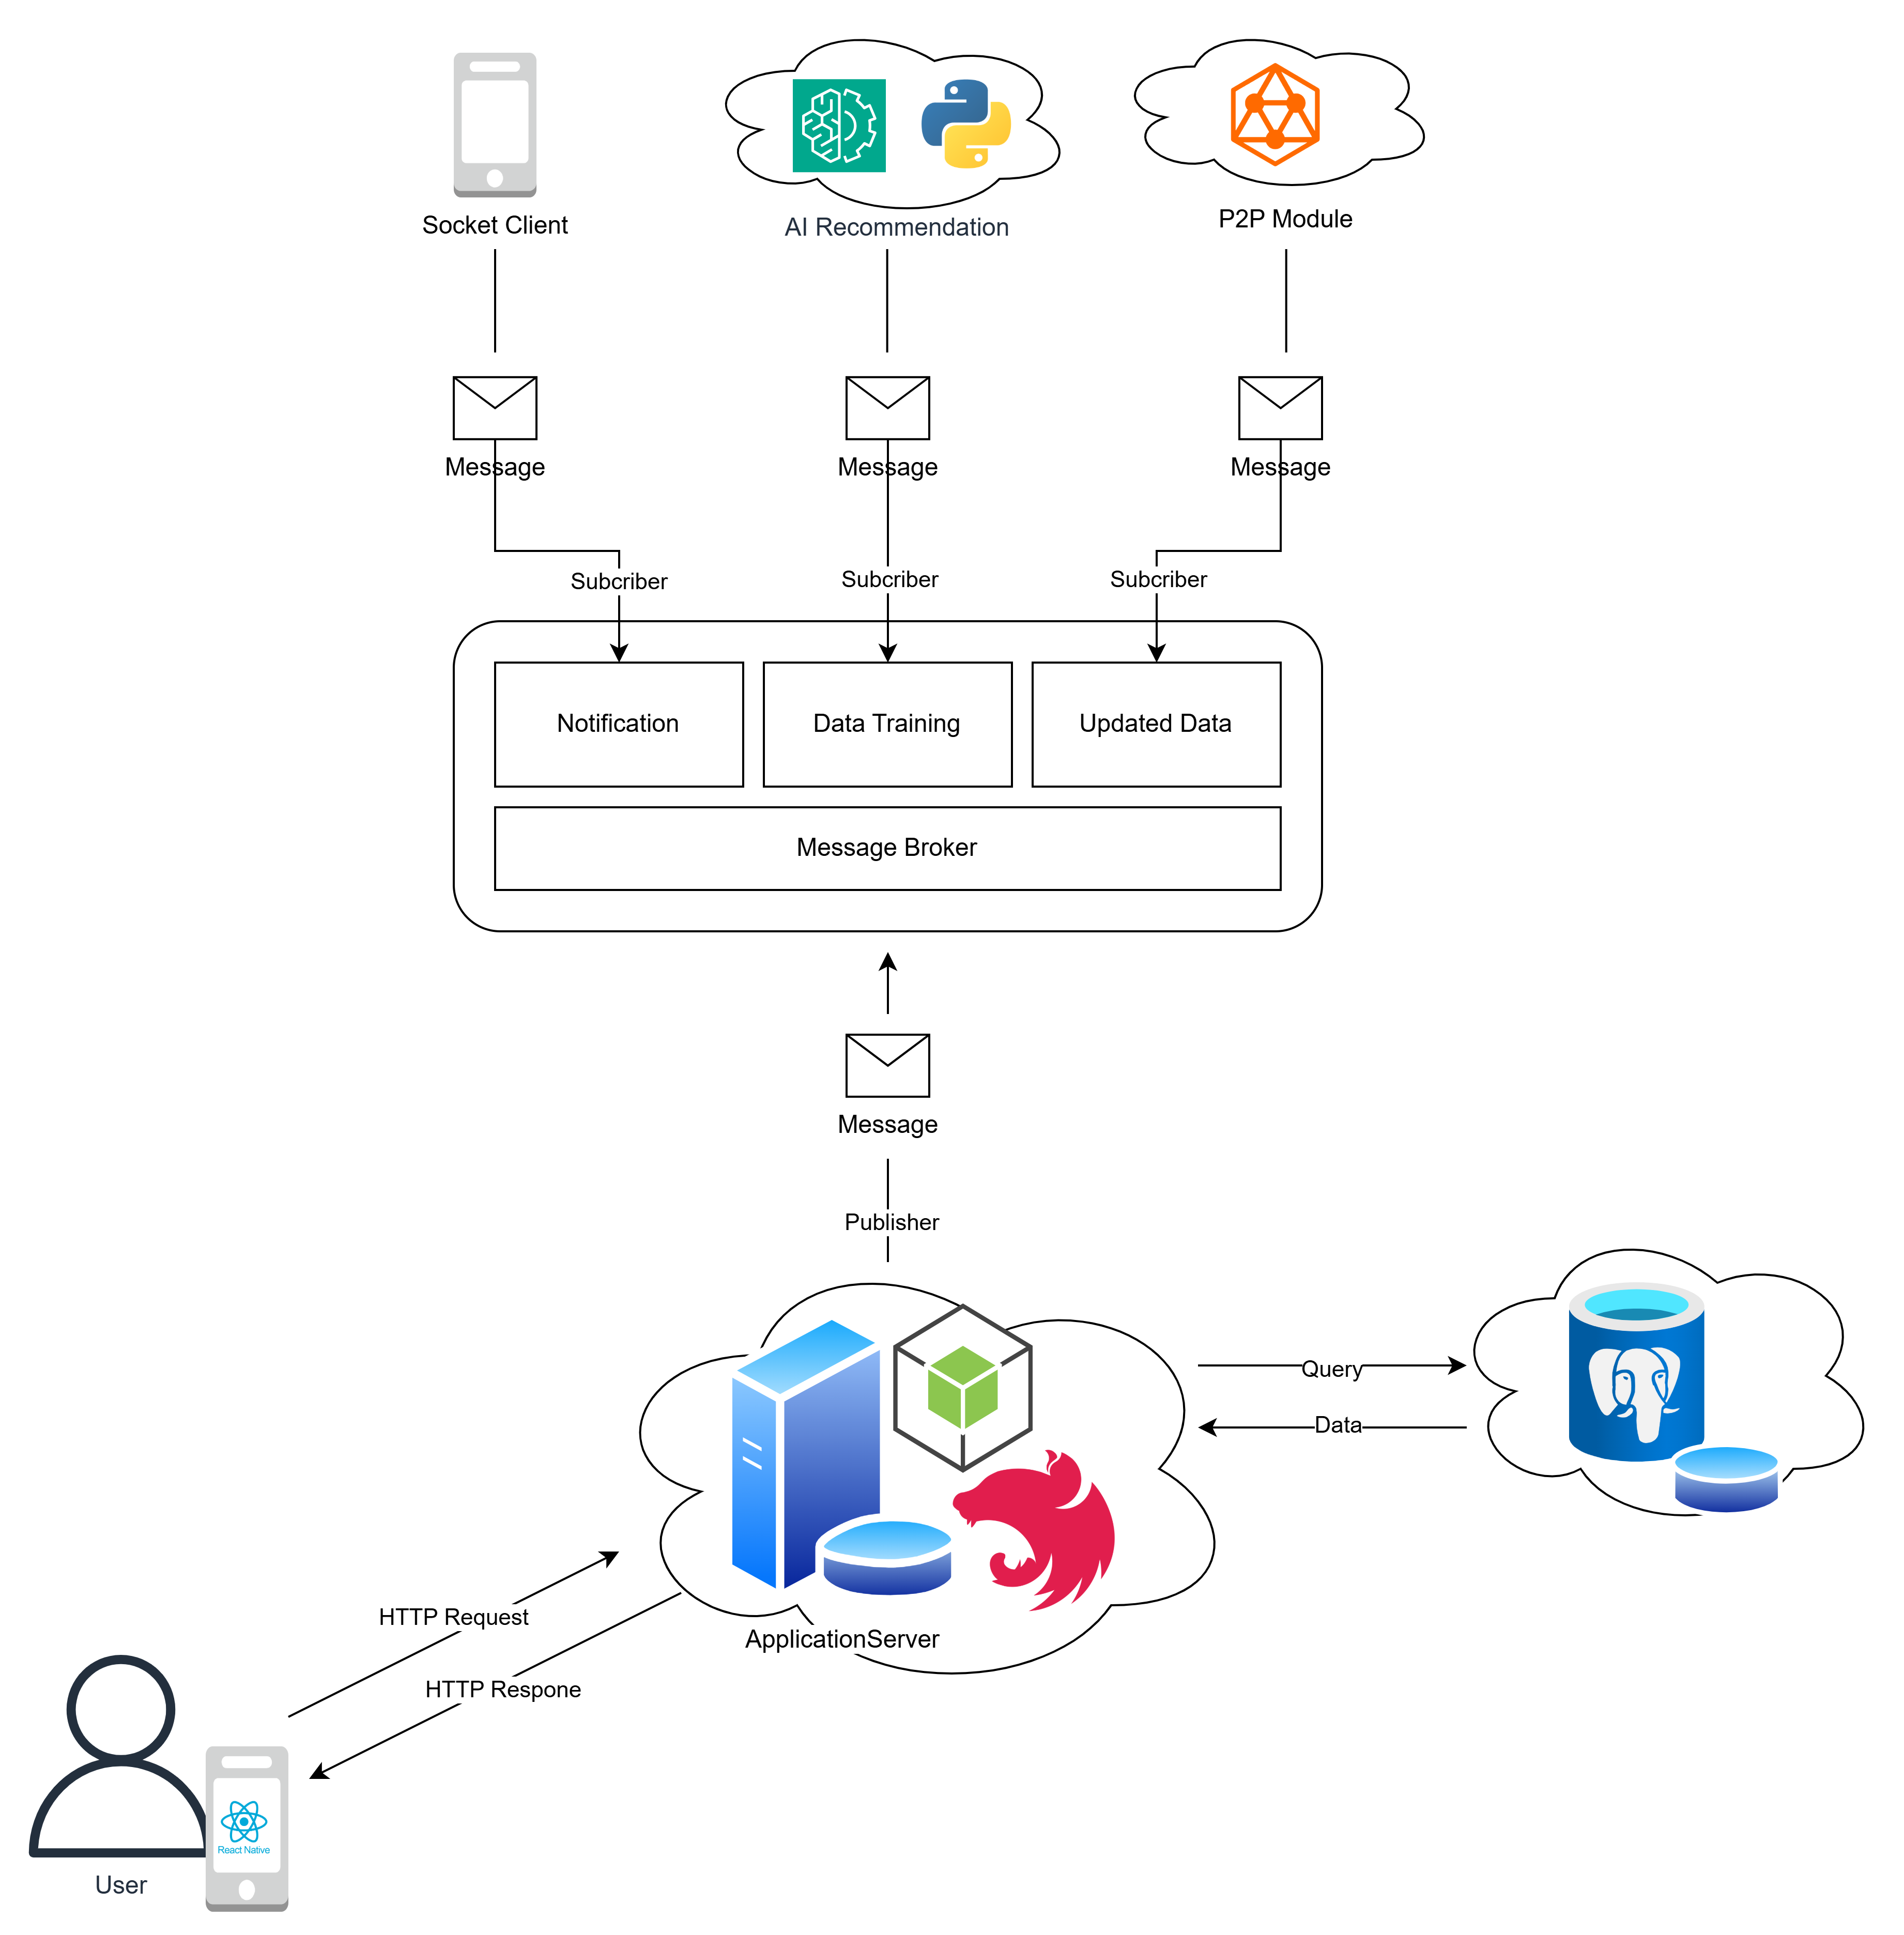
\includegraphics[width=0.7\textwidth]{Images/Deploy/arch.png}
    \caption{Deployment Diagram}
    \label{fig:deployment-diagram}
\end{figure}
\subsection{Thiết kế cơ sở dữ liệu}
\begin{figure}[H]
    \centering
    \includegraphics[width=0.95\textwidth]{Images/Design/DB/EERD.png}
    \caption{Sơ đồ cơ sở dữ liệu của hệ thống}
    \label{fig:database-diagram}
\end{figure}

\newlength{\colField} \setlength{\colField}{2.5cm}
\newlength{\colConst} \setlength{\colConst}{5.5cm}
\newlength{\colDesc}  \setlength{\colDesc}{7.0cm}

\subsubsection{Các thực thể chính}

% ==========================================
% 1. Bảng users
% ==========================================
\begin{longtable}{p{\colField} p{\colConst} p{\colDesc}}
    \caption{Bảng users (Bảng cha, Single Table Inheritance)} \label{tab:users} \\
    \toprule
    \textbf{Trường} & \textbf{Ràng buộc} & \textbf{Mô tả / Ghi chú} \\
    \midrule
    \endfirsthead
    
    \multicolumn{3}{c}{\tablename\ \thetable\ -- tiếp theo} \\
    \toprule
    \textbf{Trường} & \textbf{Ràng buộc} & \textbf{Mô tả / Ghi chú} \\
    \midrule
    \endhead
    
    \bottomrule
    \endlastfoot

    id & PK, NOT NULL & Khóa chính (UUID) \\
    full\_name & NOT NULL & Họ và tên đầy đủ \\
    email & UNIQUE, NOT NULL & Email đăng nhập hệ thống \\
    phone & UNIQUE, NOT NULL & Số điện thoại liên lạc \\
    avatar\_url & NULL & Đường dẫn ảnh đại diện \\
    password\_hash & NOT NULL & Mật khẩu đã mã hóa \\
    status & NOT NULL, default 'ACTIVE' & ENUM: ACTIVE, INACTIVE, SUSPENDED, BANNED \\
    role & NOT NULL & ENUM: RENTER, OWNER, ADMIN \\
    trust\_score & NOT NULL, default 50 & Điểm uy tín (thang 0--100) \\
    trust\_factors & NULL & JSON chi tiết các yếu tố tính điểm \\
    trust\_last\_calculated & NULL & Thời điểm tính điểm gần nhất \\
    created\_at & NOT NULL, default NOW & Thời gian tạo tài khoản \\
    updated\_at & NOT NULL, default NOW & Thời gian cập nhật lần cuối \\
\end{longtable}

\vspace{0.5cm}

% ==========================================
% 2. Bảng renters
% ==========================================
\begin{longtable}{p{\colField} p{\colConst} p{\colDesc}}
    \caption{Bảng renters (Thuộc tính riêng người thuê)} \label{tab:renters} \\
    \toprule
    \textbf{Trường} & \textbf{Ràng buộc} & \textbf{Mô tả / Ghi chú} \\
    \midrule
    \endfirsthead
    \bottomrule
    \endlastfoot

    user\_id & PK, FK $\to$ users.id, ON DELETE CASCADE & Khóa chính đồng thời là khóa ngoại \\
    address & NULL & Địa chỉ thường trú \\
    license\_number & UNIQUE, NOT NULL & Số giấy phép lái xe \\
    verification\_status & NOT NULL, default 'PENDING' & ENUM: PENDING, VERIFIED, REJECTED \\
\end{longtable}

\vspace{0.5cm}

% ==========================================
% 3. Bảng owners
% ==========================================
\begin{longtable}{p{\colField} p{\colConst} p{\colDesc}}
    \caption{Bảng owners (Thuộc tính riêng chủ xe)} \label{tab:owners} \\
    \toprule
    \textbf{Trường} & \textbf{Ràng buộc} & \textbf{Mô tả / Ghi chú} \\
    \midrule
    \endfirsthead
    \bottomrule
    \endlastfoot

    user\_id & PK, FK $\to$ users.id, ON DELETE CASCADE & Khóa chính đồng thời là khóa ngoại \\
    bank\_account & NOT NULL (encrypted) & Số tài khoản ngân hàng (nhận tiền) \\
    id\_card\_number & NOT NULL (encrypted) & Số CMND/CCCD \\
    id\_card\_front\_url & NULL & Link ảnh mặt trước CMND/CCCD \\
    id\_card\_back\_url & NULL & Link ảnh mặt sau CMND/CCCD \\
\end{longtable}

\vspace{0.5cm}

% ==========================================
% 4. Bảng admins
% ==========================================
\begin{longtable}{p{\colField} p{\colConst} p{\colDesc}}
    \caption{Bảng admins (Thuộc tính quản trị viên)} \label{tab:admins} \\
    \toprule
    \textbf{Trường} & \textbf{Ràng buộc} & \textbf{Mô tả / Ghi chú} \\
    \midrule
    \endfirsthead
    \bottomrule
    \endlastfoot

    user\_id & PK, FK $\to$ users.id, ON DELETE CASCADE & Khóa chính đồng thời là khóa ngoại \\
    permissions & NOT NULL & Danh sách quyền hạn (mảng JSON) \\
    department & NULL & Tên bộ phận quản lý \\
\end{longtable}

\vspace{0.5cm}

% ==========================================
% 5. Bảng vehicles
% ==========================================
\begin{longtable}{p{\colField} p{\colConst} p{\colDesc}}
    \caption{Bảng vehicles (Thông tin xe)} \label{tab:vehicles} \\
    \toprule
    \textbf{Trường} & \textbf{Ràng buộc} & \textbf{Mô tả / Ghi chú} \\
    \midrule
    \endfirsthead
    \multicolumn{3}{c}{\tablename\ \thetable\ -- tiếp theo} \\
    \toprule
    \textbf{Trường} & \textbf{Ràng buộc} & \textbf{Mô tả / Ghi chú} \\
    \midrule
    \endhead
    \bottomrule
    \endlastfoot

    id & PK & Khóa chính (UUID) \\
    owner\_id & FK $\to$ users.id (role=OWNER), NOT NULL & Liên kết tới chủ sở hữu \\
    license\_plate & UNIQUE, NOT NULL & Biển số xe \\
    model & NOT NULL & Tên mẫu xe (Model) \\
    type & NOT NULL & ENUM: STANDARD, PREMIUM, HEAVY\_DUTY \\
    status & NOT NULL & ENUM: AVAILABLE, RENTED, MAINTENANCE, INACTIVE... \\
    battery\_level & NOT NULL, range 0--100 & Phần trăm pin hiện tại \\
    price\_per\_hour & NOT NULL & Đơn giá thuê theo giờ \\
    latitude & NOT NULL & Vĩ độ vị trí hiện tại \\
    longitude & NOT NULL & Kinh độ vị trí hiện tại \\
    total\_rating & default 0 & Điểm đánh giá trung bình \\
    total\_trips & default 0 & Tổng số chuyến đi đã thực hiện \\
    image\_urls & NULL & Mảng JSON chứa link ảnh xe \\
    created\_at & NOT NULL, default NOW & Thời gian đăng ký xe \\
\end{longtable}

\vspace{0.5cm}

% ==========================================
% 6. Bảng bookings
% ==========================================
\begin{longtable}{p{\colField} p{\colConst} p{\colDesc}}
    \caption{Bảng bookings (Đơn đặt xe)} \label{tab:bookings} \\
    \toprule
    \textbf{Trường} & \textbf{Ràng buộc} & \textbf{Mô tả / Ghi chú} \\
    \midrule
    \endfirsthead
    \multicolumn{3}{c}{\tablename\ \thetable\ -- tiếp theo} \\
    \toprule
    \textbf{Trường} & \textbf{Ràng buộc} & \textbf{Mô tả / Ghi chú} \\
    \midrule
    \endhead
    \bottomrule
    \endlastfoot

    id & PK & Khóa chính (UUID) \\
    renter\_id & FK $\to$ users.id (role=RENTER), NOT NULL & Người thực hiện thuê \\
    vehicle\_id & FK $\to$ vehicles.id, NOT NULL & Xe được chọn thuê \\
    start\_time & NOT NULL & Thời gian bắt đầu thuê \\
    end\_time & NOT NULL & Thời gian kết thúc dự kiến \\
    actual\_end\_time & NULL & Thời gian trả xe thực tế \\
    status & NOT NULL & ENUM: PENDING, APPROVED, ON\_TRIP, COMPLETED... \\
    total\_cost & NOT NULL & Tổng chi phí chuyến đi \\
    deposit & NOT NULL & Số tiền đặt cọc giữ xe \\
    start\_latitude & NOT NULL & Vĩ độ điểm nhận xe \\
    start\_longitude & NOT NULL & Kinh độ điểm nhận xe \\
    end\_latitude & NULL & Vĩ độ điểm trả xe \\
    end\_longitude & NULL & Kinh độ điểm trả xe \\
    created\_at & NOT NULL, default NOW & Thời gian tạo đơn \\
    updated\_at & NOT NULL, default NOW & Thời gian cập nhật trạng thái \\
\end{longtable}

\vspace{0.5cm}

% ==========================================
% 7. Bảng payments
% ==========================================
\begin{longtable}{p{\colField} p{\colConst} p{\colDesc}}
    \caption{Bảng payments (Giao dịch thanh toán)} \label{tab:payments} \\
    \toprule
    \textbf{Trường} & \textbf{Ràng buộc} & \textbf{Mô tả / Ghi chú} \\
    \midrule
    \endfirsthead
    \bottomrule
    \endlastfoot

    id & PK & Khóa chính (UUID) \\
    booking\_id & FK $\to$ bookings.id, NOT NULL & Liên kết đơn hàng \\
    transaction\_id & UNIQUE & Mã tham chiếu từ cổng thanh toán \\
    amount & NOT NULL & Số tiền giao dịch \\
    method & NOT NULL & ENUM: CARD, E\_WALLET, BANK\_TRANSFER \\
    status & NOT NULL & ENUM: PENDING, COMPLETED, FAILED, REFUNDED \\
    processed\_at & NULL & Thời điểm xử lý xong \\
    failure\_reason & NULL & Lý do thất bại (nếu có) \\
\end{longtable}

\vspace{0.5cm}

% ==========================================
% 8. Bảng reviews
% ==========================================
\begin{longtable}{p{\colField} p{\colConst} p{\colDesc}}
    \caption{Bảng reviews (Đánh giá chuyến đi)} \label{tab:reviews} \\
    \toprule
    \textbf{Trường} & \textbf{Ràng buộc} & \textbf{Mô tả / Ghi chú} \\
    \midrule
    \endfirsthead
    \bottomrule
    \endlastfoot

    id & PK & Khóa chính (UUID) \\
    booking\_id & FK $\to$ bookings.id, UNIQUE, NOT NULL & Mỗi chuyến đi chỉ có 1 đánh giá \\
    rating & NOT NULL, range 1--5 & Số sao đánh giá \\
    comment & NULL & Nội dung nhận xét chi tiết \\
    is\_pending & NOT NULL, default TRUE & Cờ báo trạng thái chờ duyệt \\
    created\_at & NOT NULL, default NOW & Thời gian viết đánh giá \\
\end{longtable}

\vspace{0.5cm}

% ==========================================
% 9. Bảng issues
% ==========================================
\begin{longtable}{p{\colField} p{\colConst} p{\colDesc}}
    \caption{Bảng issues (Báo cáo sự cố)} \label{tab:issues} \\
    \toprule
    \textbf{Trường} & \textbf{Ràng buộc} & \textbf{Mô tả / Ghi chú} \\
    \midrule
    \endfirsthead
    \bottomrule
    \endlastfoot

    id & PK & Khóa chính (UUID) \\
    booking\_id & FK $\to$ bookings.id, NOT NULL & Liên kết đơn thuê xảy ra sự cố \\
    vehicle\_id & FK $\to$ vehicles.id, NOT NULL & Xe gặp sự cố \\
    reported\_by & FK $\to$ users.id, NOT NULL & Người báo cáo \\
    type & NOT NULL & Loại sự cố (hỏng hóc, tai nạn...) \\
    description & NOT NULL & Mô tả chi tiết sự việc \\
    status & NOT NULL & ENUM: OPEN, IN\_PROGRESS, RESOLVED \\
    created\_at & NOT NULL, default NOW & Thời gian báo cáo \\
    resolved\_at & NULL & Thời gian giải quyết xong \\
\end{longtable}

\vspace{0.5cm}

% ==========================================
% 10. Bảng notifications
% ==========================================
\begin{longtable}{p{\colField} p{\colConst} p{\colDesc}}
    \caption{Bảng notifications (Hệ thống thông báo)} \label{tab:notifications} \\
    \toprule
    \textbf{Trường} & \textbf{Ràng buộc} & \textbf{Mô tả / Ghi chú} \\
    \midrule
    \endfirsthead
    \bottomrule
    \endlastfoot

    id & PK & Khóa chính (UUID) \\
    user\_id & FK $\to$ users.id, NOT NULL & Người nhận thông báo \\
    type & NOT NULL & Loại: BOOKING\_REQUEST, PROMOTION... \\
    title & NOT NULL & Tiêu đề thông báo \\
    message & NOT NULL & Nội dung thông báo \\
    data & NULL & Dữ liệu JSON bổ sung (để điều hướng app) \\
    is\_read & NOT NULL, default FALSE & Trạng thái đã xem \\
    sent\_at & NOT NULL, default NOW & Thời gian gửi \\
\end{longtable}

\vspace{0.5cm}

% ==========================================
% 11. Bảng analytics_reports
% ==========================================
\begin{longtable}{p{\colField} p{\colConst} p{\colDesc}}
    \caption{Bảng analytics\_reports (Báo cáo thống kê)} \label{tab:analytics} \\
    \toprule
    \textbf{Trường} & \textbf{Ràng buộc} & \textbf{Mô tả / Ghi chú} \\
    \midrule
    \endfirsthead
    \bottomrule
    \endlastfoot

    id & PK & Khóa chính (UUID) \\
    admin\_id & FK $\to$ users.id (role=ADMIN), NOT NULL & Người tạo báo cáo \\
    start\_date & NOT NULL & Ngày bắt đầu kỳ báo cáo \\
    end\_date & NOT NULL & Ngày kết thúc kỳ báo cáo \\
    total\_revenue & NOT NULL & Tổng doanh thu trong kỳ \\
    total\_bookings & NOT NULL & Tổng số đơn hàng \\
    total\_issues & NOT NULL & Tổng số sự cố ghi nhận \\
    vehicle\_distribution & NULL & JSON phân bố xe theo loại \\
    created\_at & NOT NULL, default NOW & Thời gian tạo báo cáo \\
\end{longtable}

% \subsubsection{Quan hệ giữa các thực thể}
% \begin{itemize}
%     \item \textbf{users -- notifications (1:N)} \quad user\_id (FK, NOT NULL)
%     \item \textbf{users (role=ADMIN) -- analytics\_reports (1:N)} \quad admin\_id (FK)
%     \item \textbf{users (role=OWNER) -- vehicles (1:N)} \quad owner\_id (FK, NOT NULL)
%     \item \textbf{users (role=RENTER) -- bookings (1:N)} \quad renter\_id (FK, NOT NULL)
%     \item \textbf{vehicles -- bookings (1:N)} \quad vehicle\_id (FK, NOT NULL)
%     \item \textbf{bookings -- payments (1:N)} \quad booking\_id (FK, NOT NULL)
%     \item \textbf{bookings -- reviews (1:1)} \quad booking\_id (FK, UNIQUE, NOT NULL)
%     \item \textbf{bookings -- issues (1:N)} \quad booking\_id (FK, NOT NULL)
%     \item \textbf{Mối quan hệ kế thừa}: Mỗi user thuộc đúng một trong ba bảng renters, owners hoặc admins thông qua user\_id (FK, PK của bảng con).
% \end{itemize}

% \begin{figure}[H]
%     \centering
%     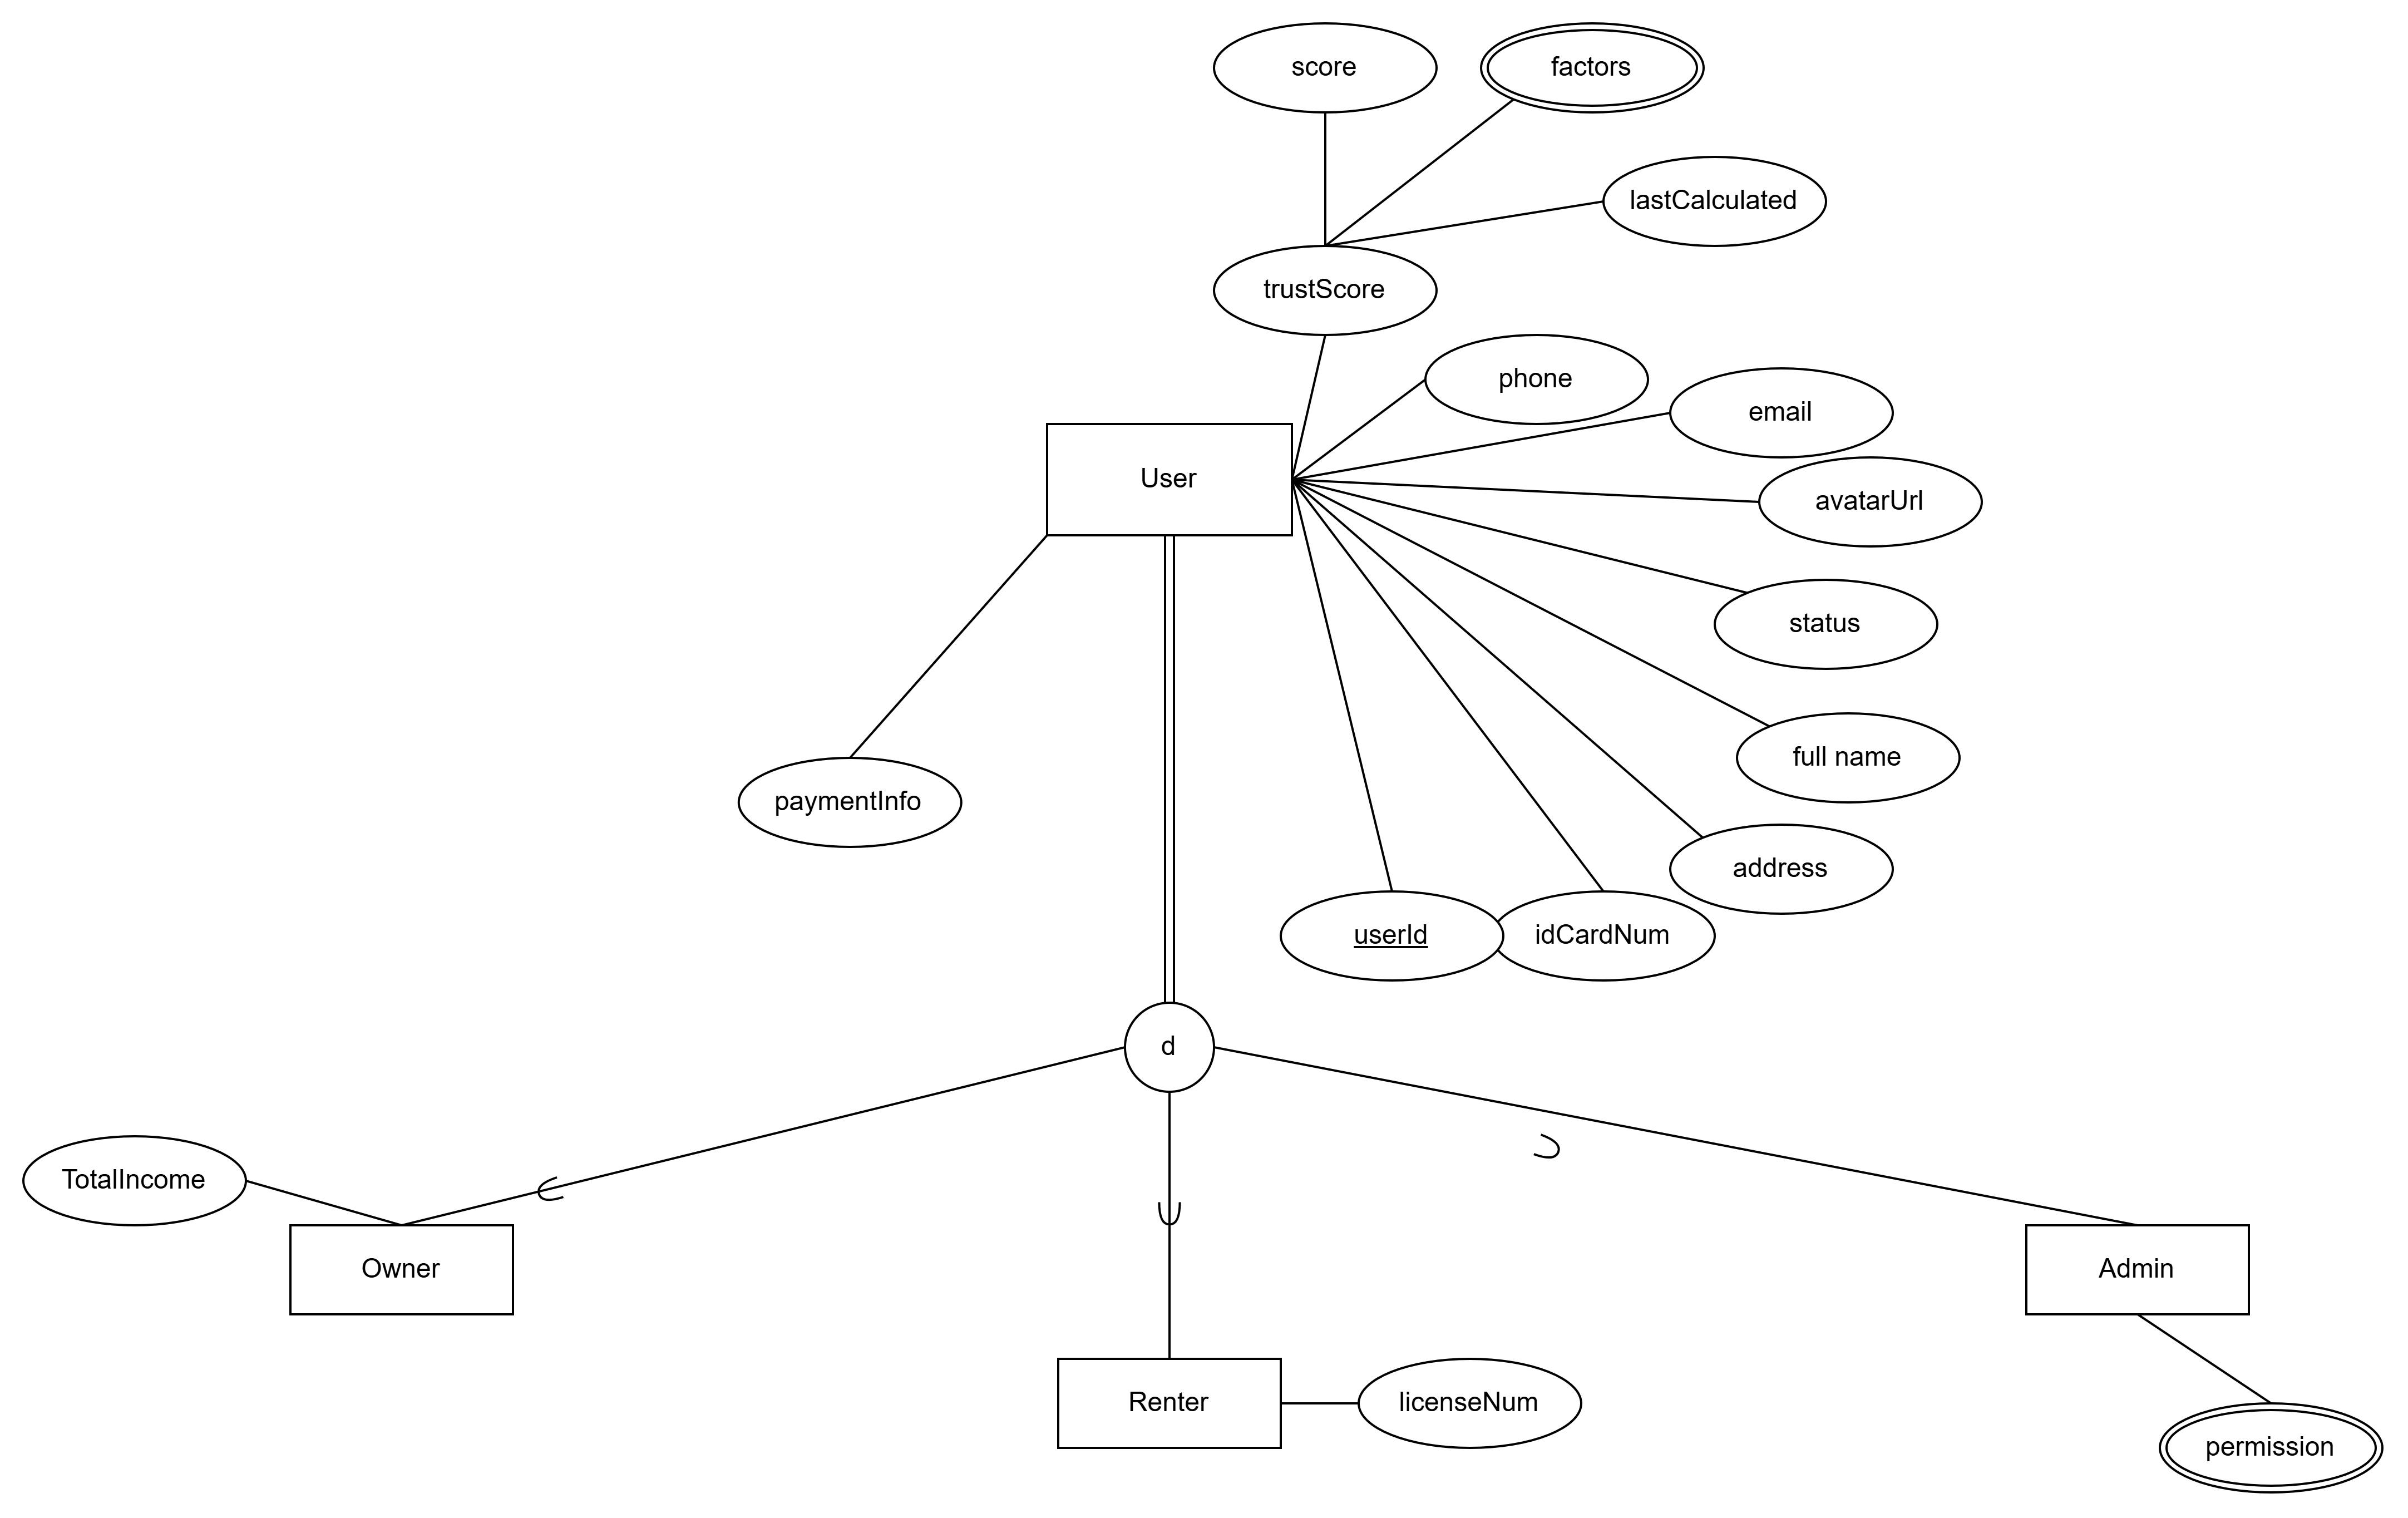
\includegraphics[width=0.6\textwidth]{Images/Design/DB/user.png}
%     \caption{Quan hệ kế thừa giữa users với renters, owners, admins}
%     \label{fig:rel-inheritance}
% \end{figure}

\subsubsection{Quan hệ giữa các thực thể}

\textbf{(1) User -- Notification (1:N)} \\[4pt]
Mỗi \texttt{Notification} phải thuộc về đúng một \texttt{User} (tham gia bắt buộc). 
Một \texttt{User} có thể có không hoặc nhiều thông báo (0..N). 
Triển khai bằng foreign key \texttt{userId} trong bảng \texttt{Notification} với constraint NOT NULL.

\begin{figure}[H]
    \centering
    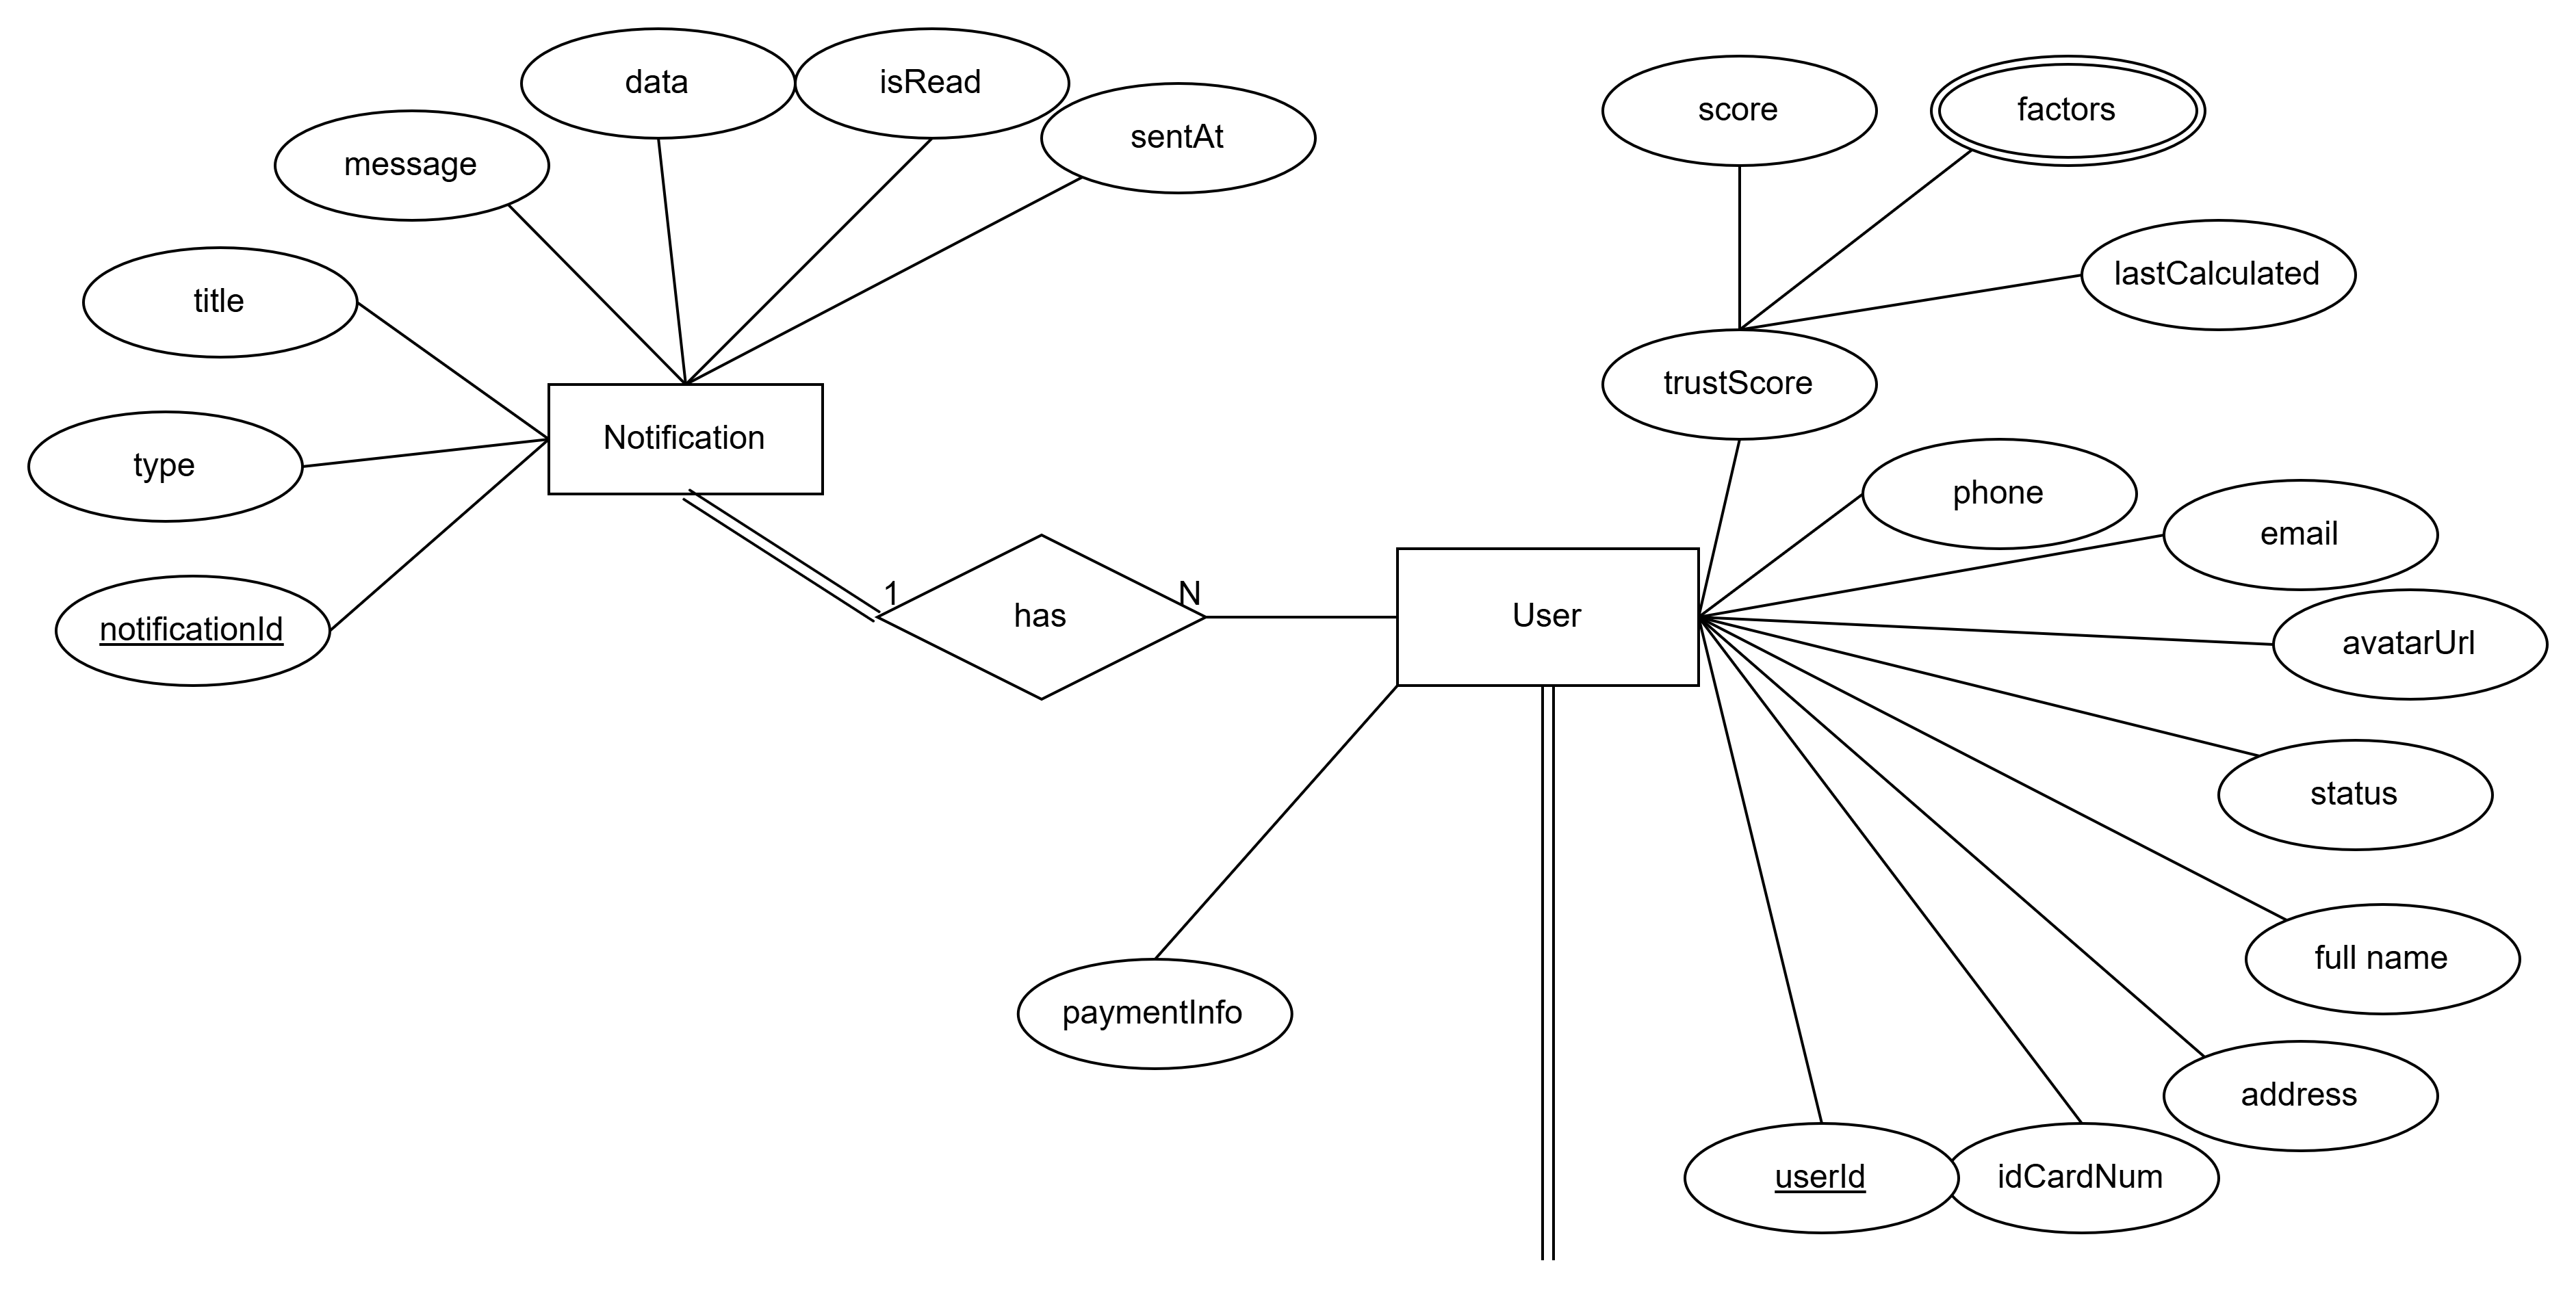
\includegraphics[width=0.8\textwidth]{Images/Design/DB/user-notify.png}
    \caption{Quan hệ giữa \texttt{User} và \texttt{Notification} (1:N)}
    \label{fig:rel-user-notification}
\end{figure}

\vspace{10pt}

\textbf{(2) Admin -- AnalyticsReport (1:N)} \\[4pt]
Mỗi \texttt{AnalyticsReport} được tạo bởi đúng một \texttt{Admin} (tham gia bắt buộc). 
Một \texttt{Admin} có thể tạo nhiều báo cáo hoặc chưa tạo báo cáo nào (0..N). 
Foreign key \texttt{adminId} trong bảng \texttt{AnalyticsReport}.

\begin{figure}[H]
    \centering
    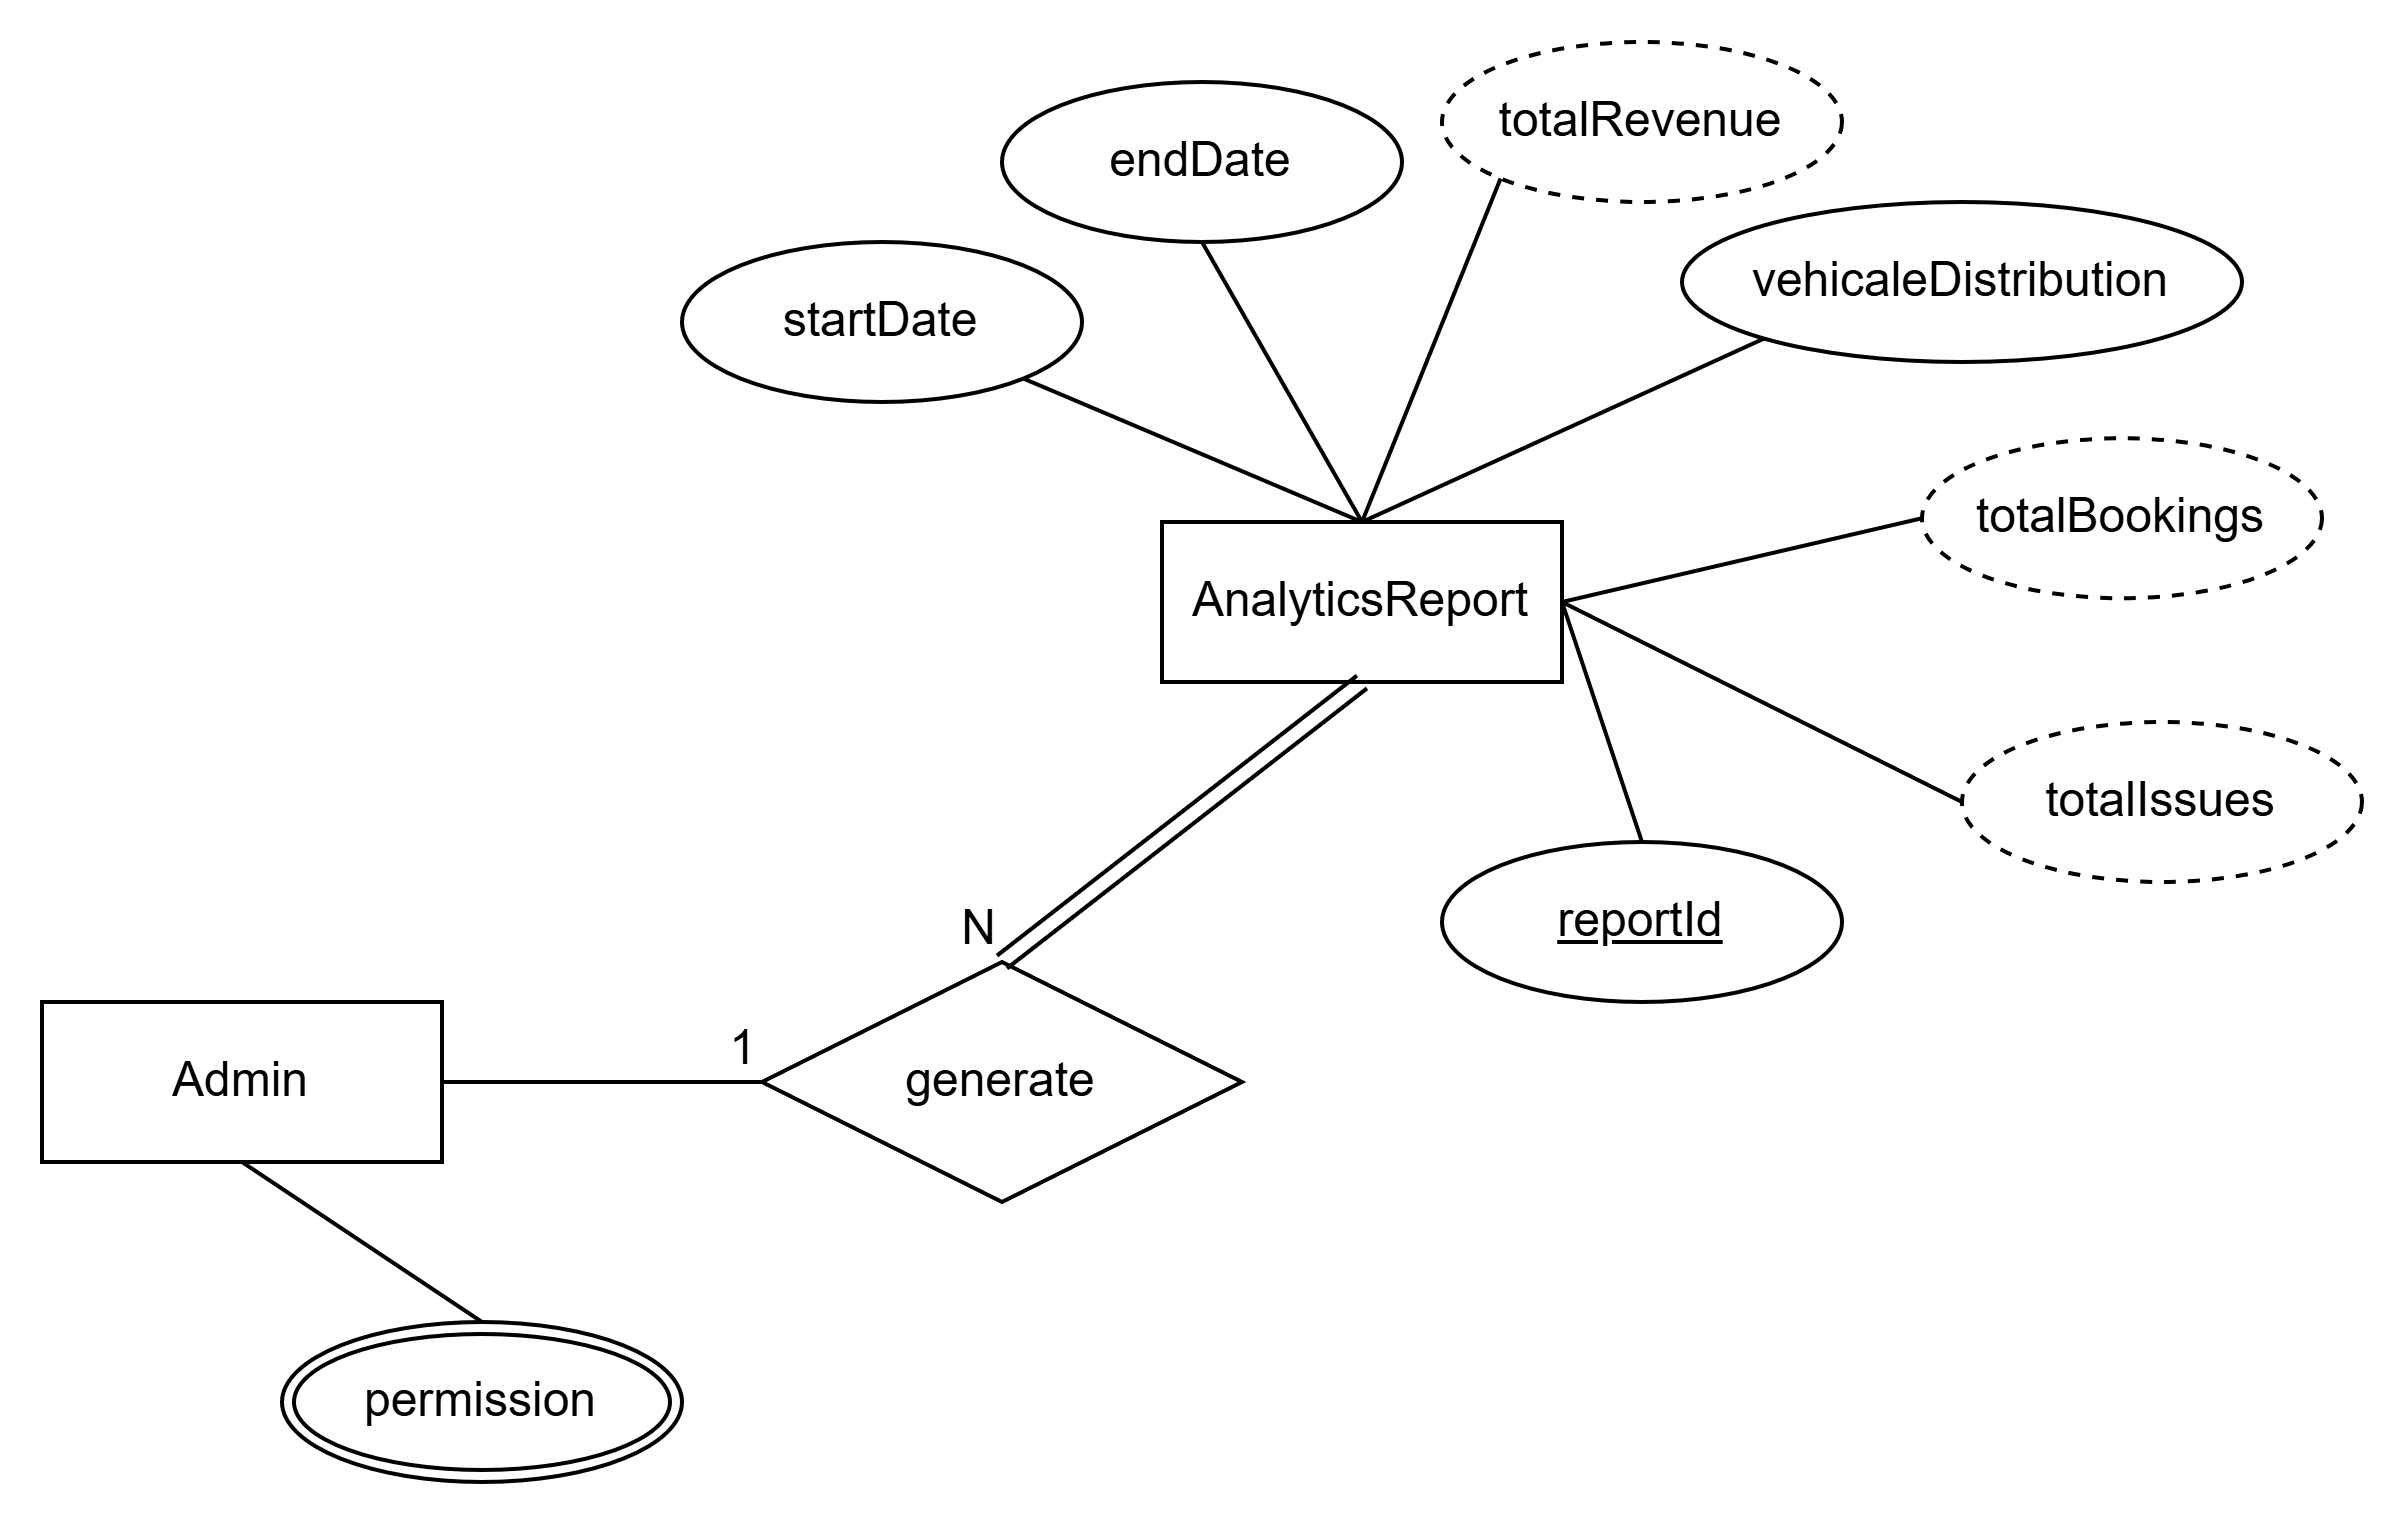
\includegraphics[width=0.8\textwidth]{Images/Design/DB/admin-report.png}
    \caption{Quan hệ giữa \texttt{Admin} và \texttt{AnalyticsReport} (1:N)}
    \label{fig:rel-admin-report}
\end{figure}

\vspace{10pt}

\textbf{(3) Owner -- Vehicle (1:N)} \\[4pt]
Mỗi \texttt{Vehicle} phải thuộc về đúng một \texttt{Owner} (tham gia bắt buộc). 
Một \texttt{Owner} có thể sở hữu nhiều xe hoặc chưa có xe nào (0..N). 
Foreign key \texttt{ownerId} trong bảng \texttt{Vehicle} với constraint NOT NULL.

\begin{figure}[H]
    \centering
    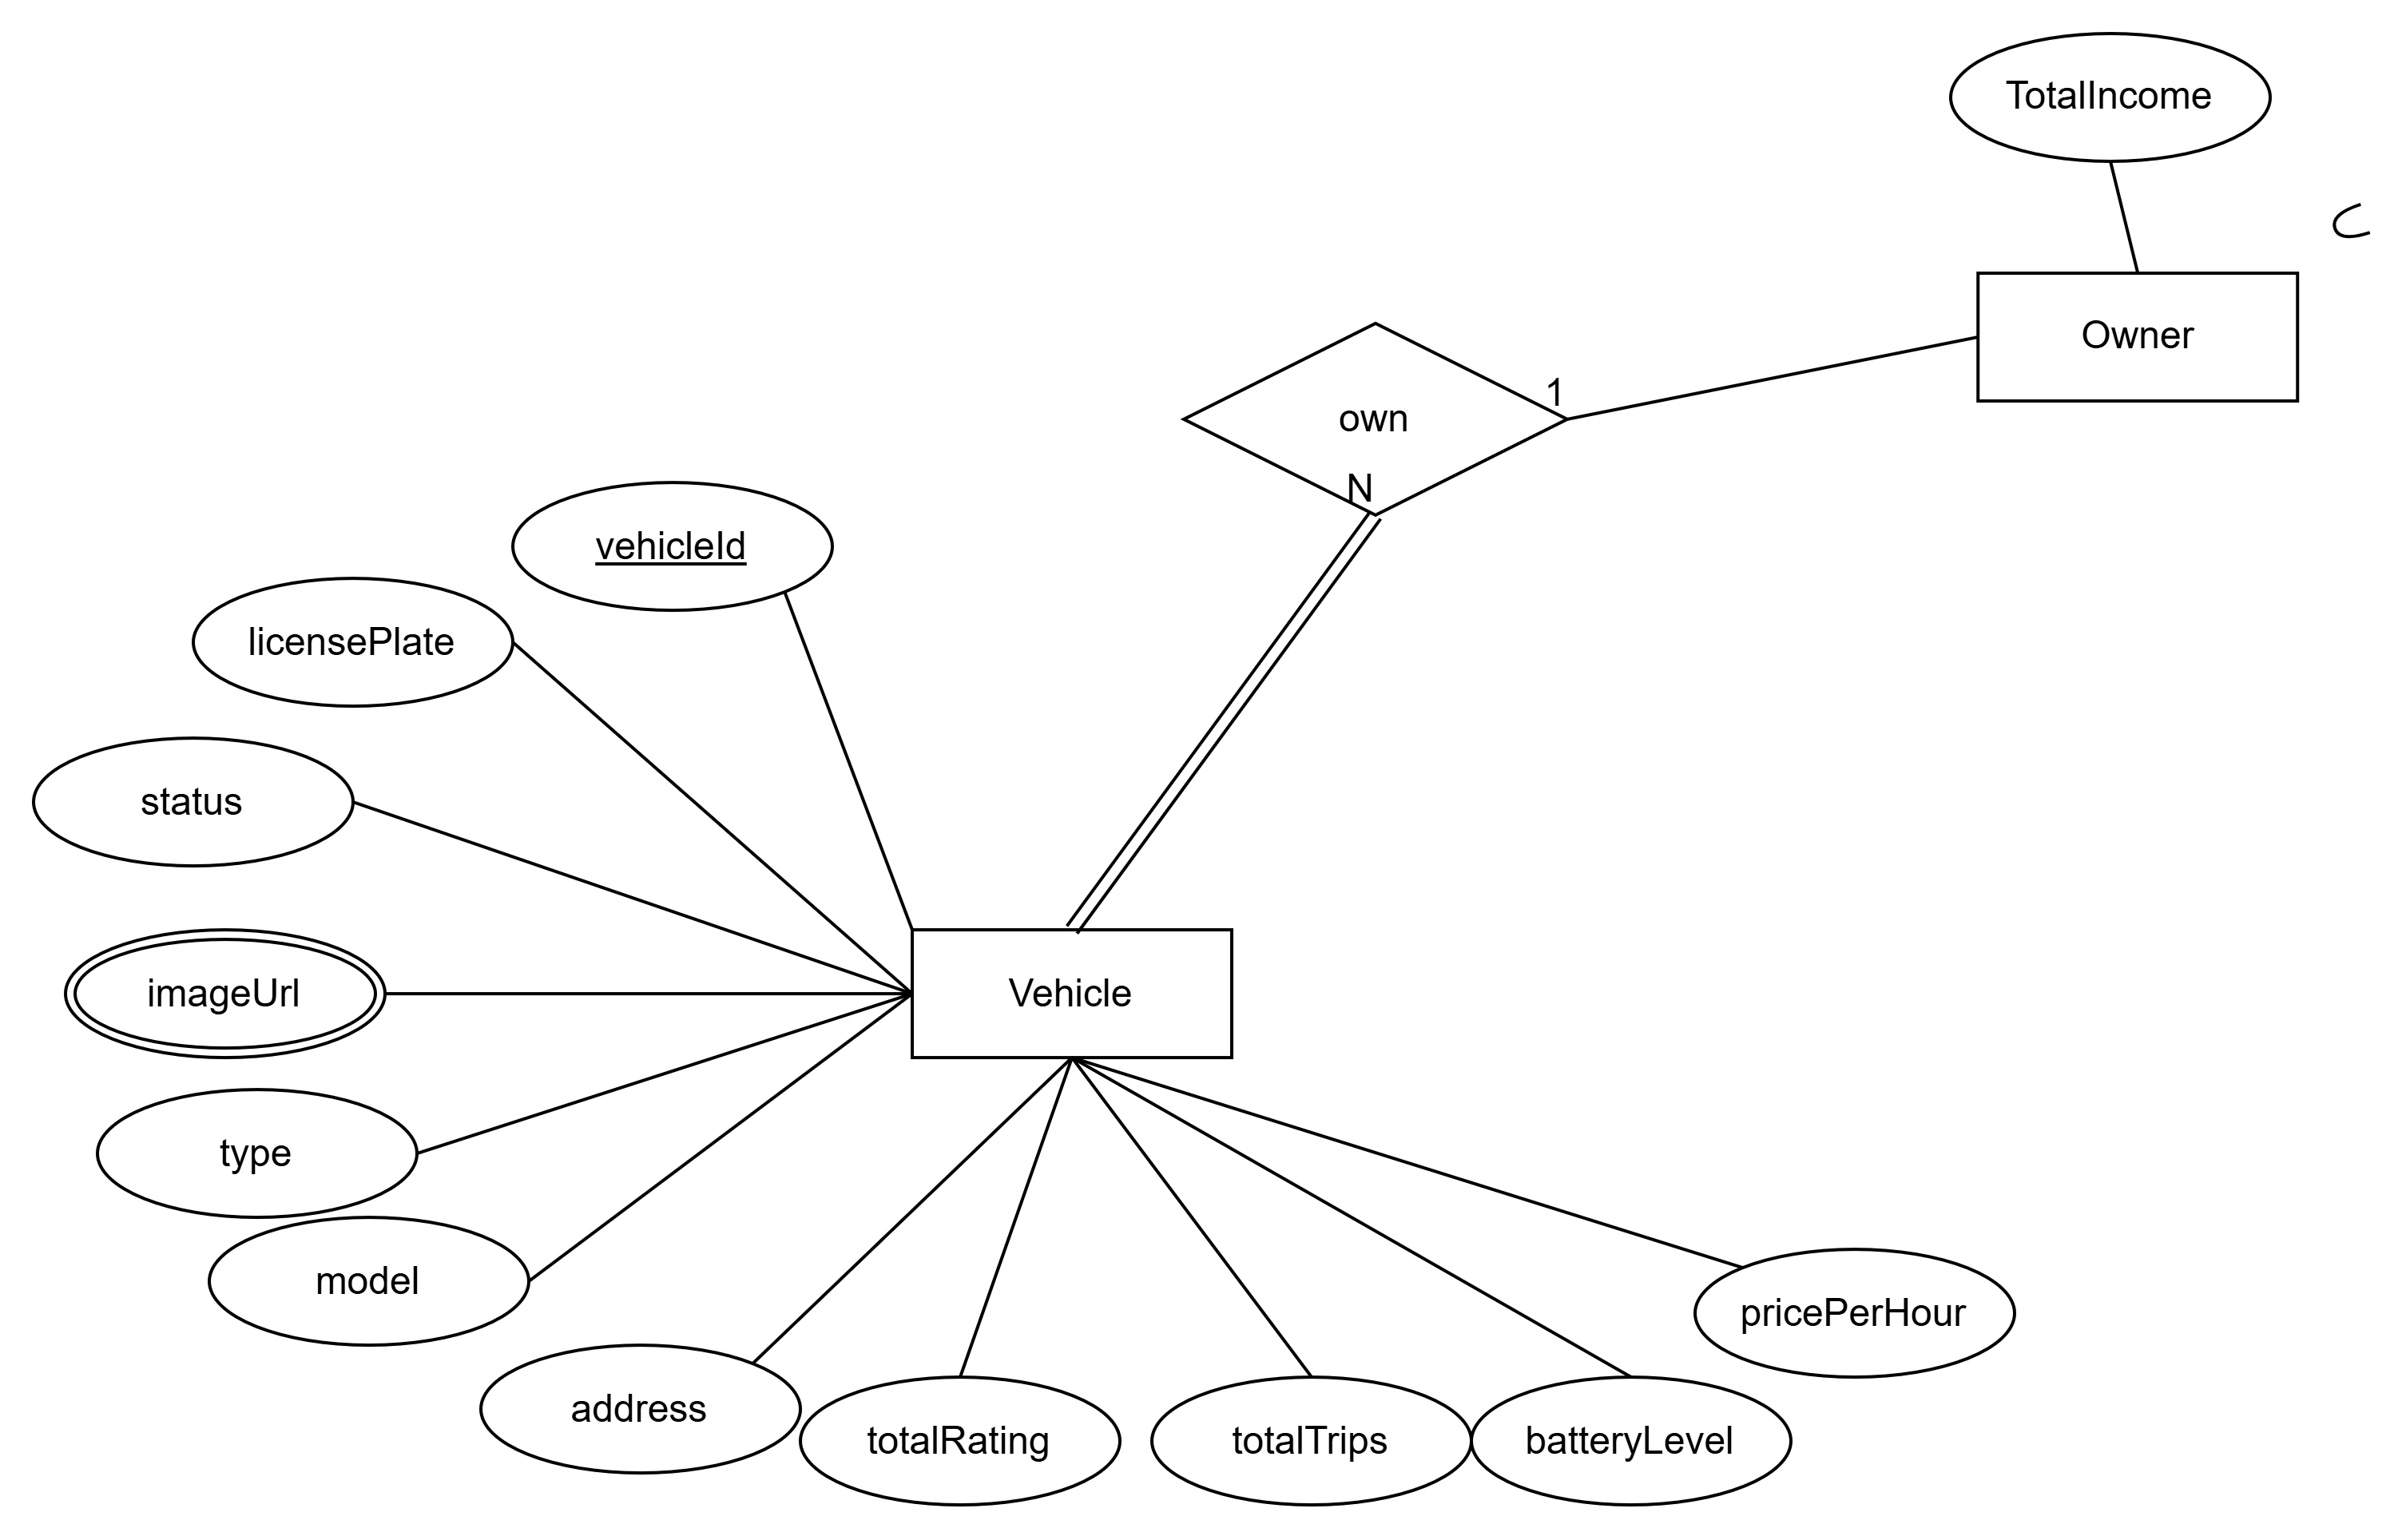
\includegraphics[width=0.8\textwidth]{Images/Design/DB/owner-vehicle.png}
    \caption{Quan hệ giữa \texttt{Owner} và \texttt{Vehicle} (1:N)}
    \label{fig:rel-owner-vehicle}
\end{figure}

\vspace{10pt}

\textbf{(4) Renter -- Booking (1:N)} \\[4pt]
Mỗi \texttt{Booking} được tạo bởi đúng một \texttt{Renter} (tham gia bắt buộc). 
Một \texttt{Renter} có thể tạo nhiều booking hoặc chưa có booking nào (0..N). 
Foreign key \texttt{renterId} trong bảng \texttt{Booking} với constraint NOT NULL.

\begin{figure}[H]
    \centering
    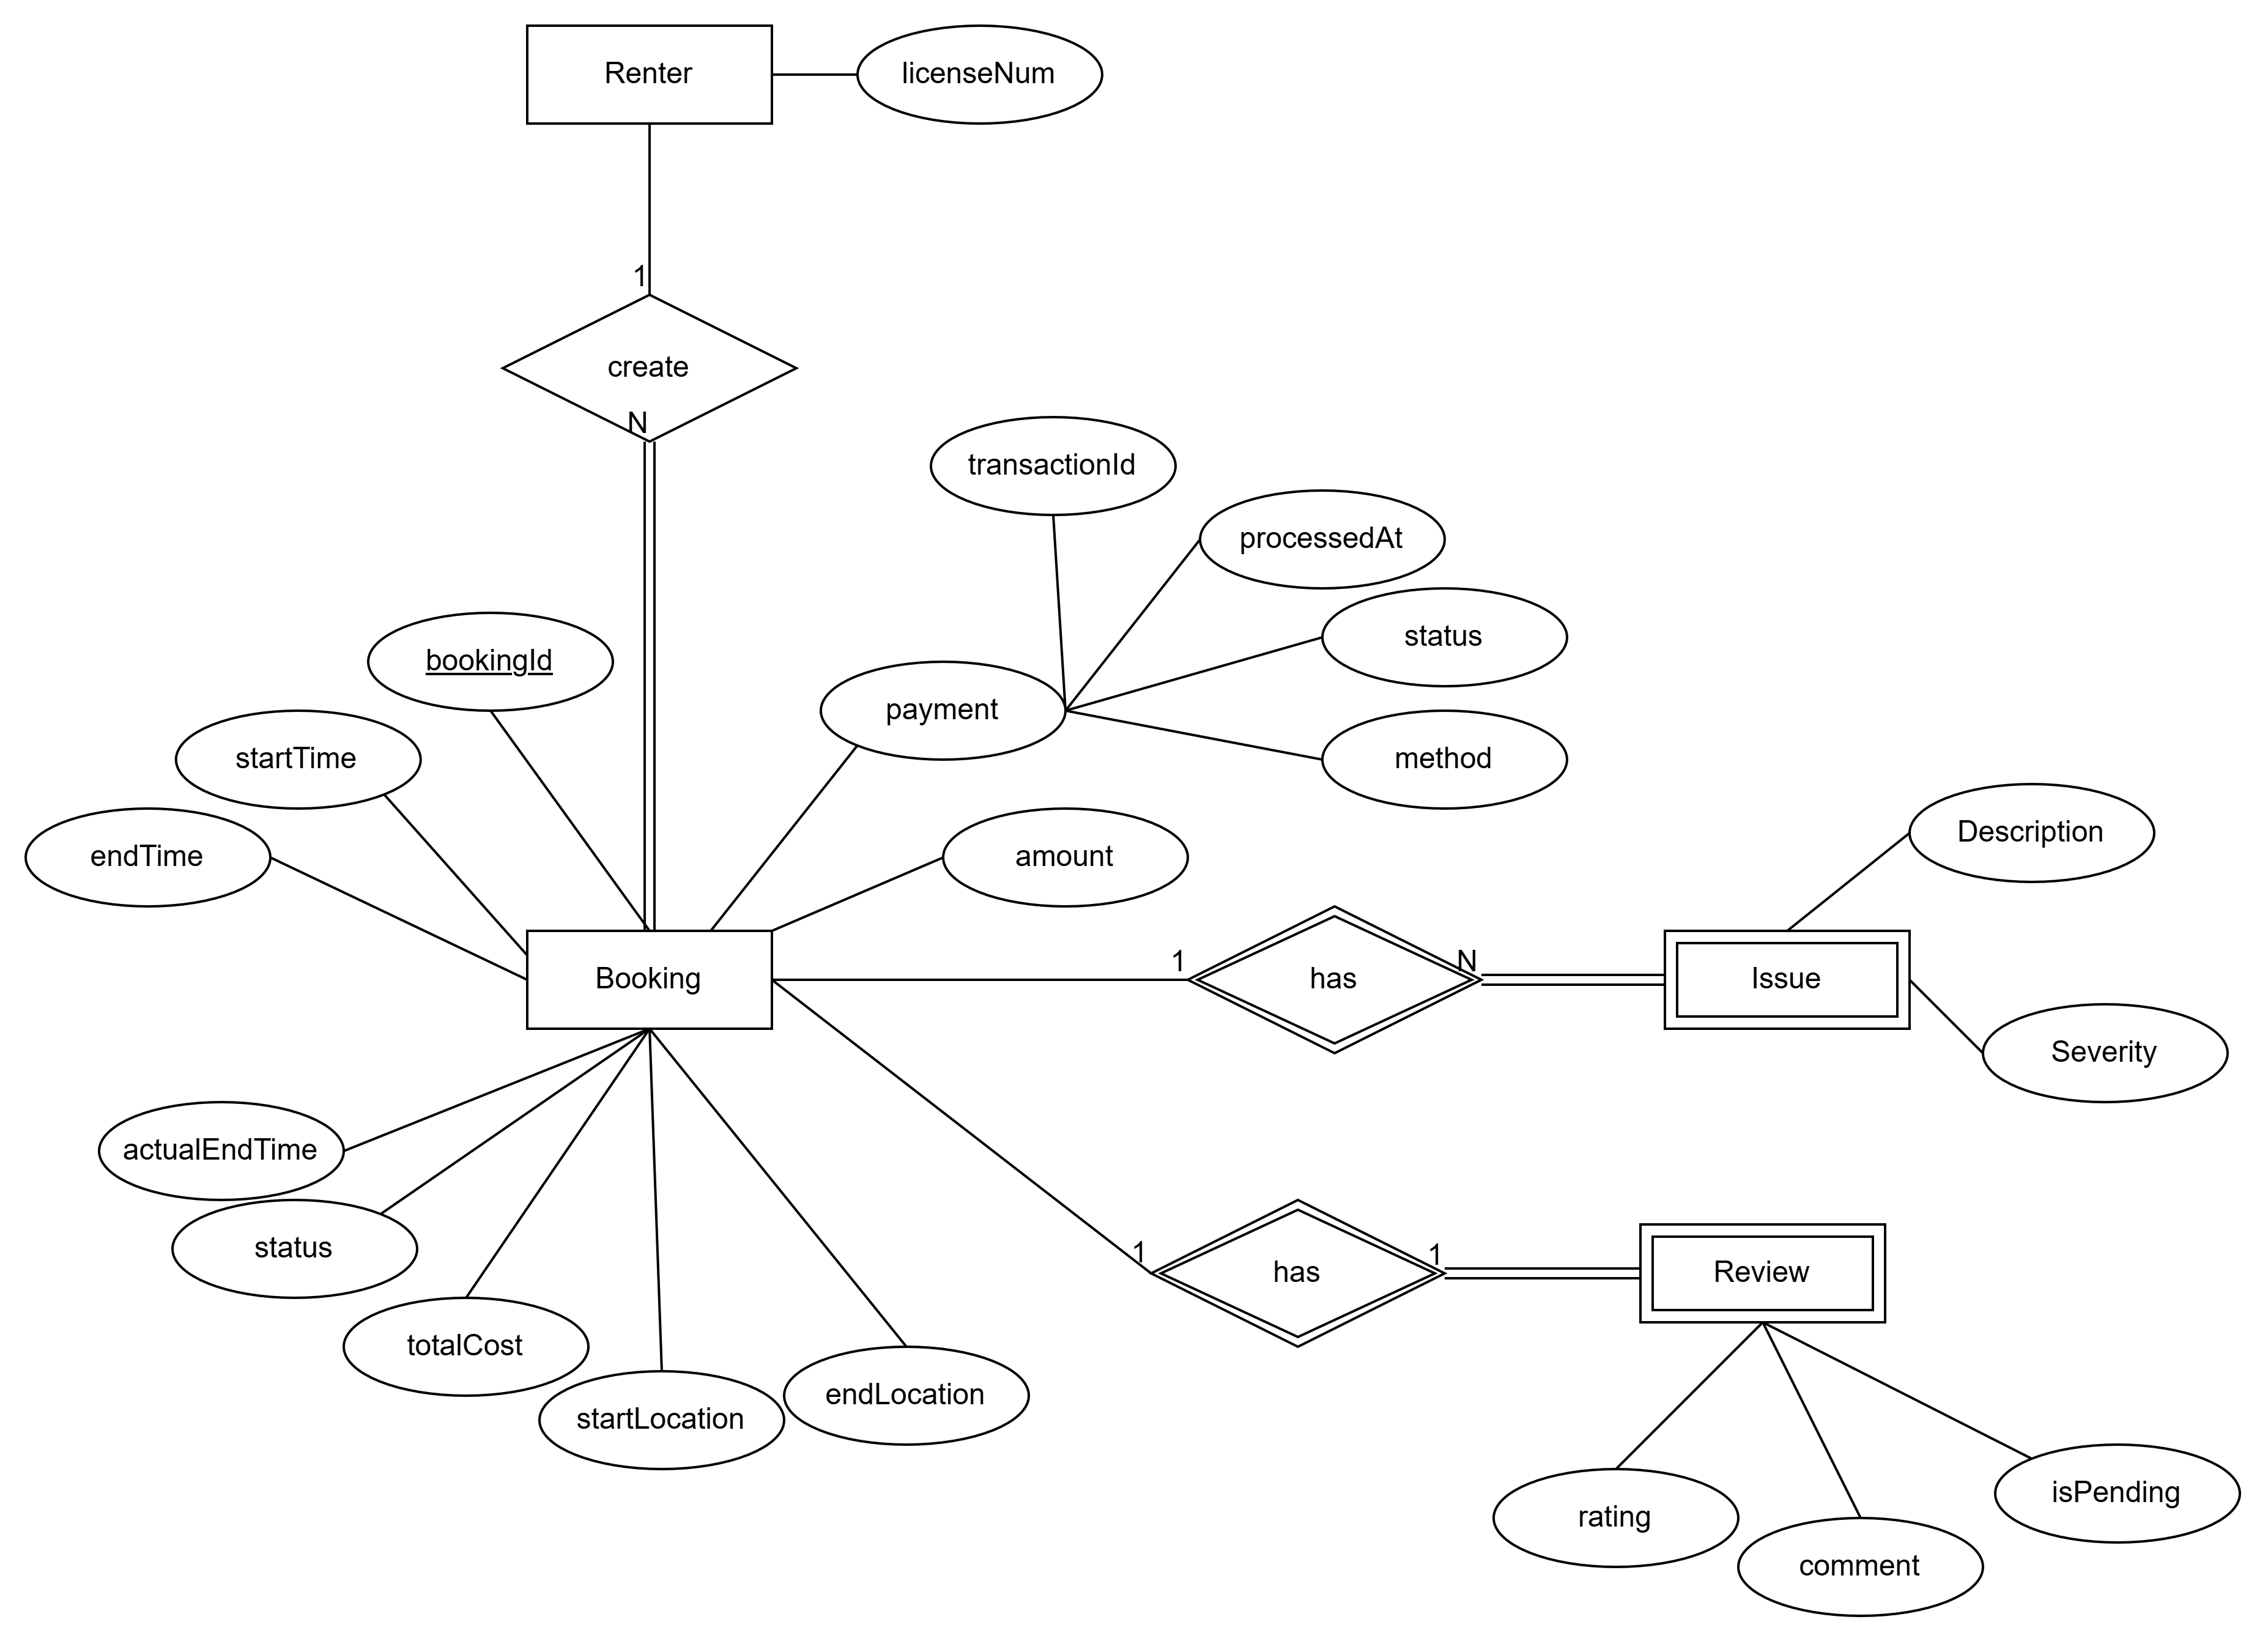
\includegraphics[width=0.8\textwidth]{Images/Design/DB/renter-booking.png}
    \caption{Quan hệ giữa \texttt{Renter} và \texttt{Booking} (1:N)}
    \label{fig:rel-renter-booking}
\end{figure}

\vspace{10pt}

\textbf{(5) Vehicle -- Booking (1:N)} \\[4pt]
Mỗi \texttt{Booking} phải gắn với đúng một \texttt{Vehicle} (tham gia bắt buộc). 
Một \texttt{Vehicle} có thể có nhiều booking hoặc chưa được thuê (0..N). 
Foreign key \texttt{vehicleId} trong bảng \texttt{Booking} với constraint NOT NULL. 
Hỗ trợ kiểm tra xung đột thời gian thuê xe.

\begin{figure}[H]
    \centering
    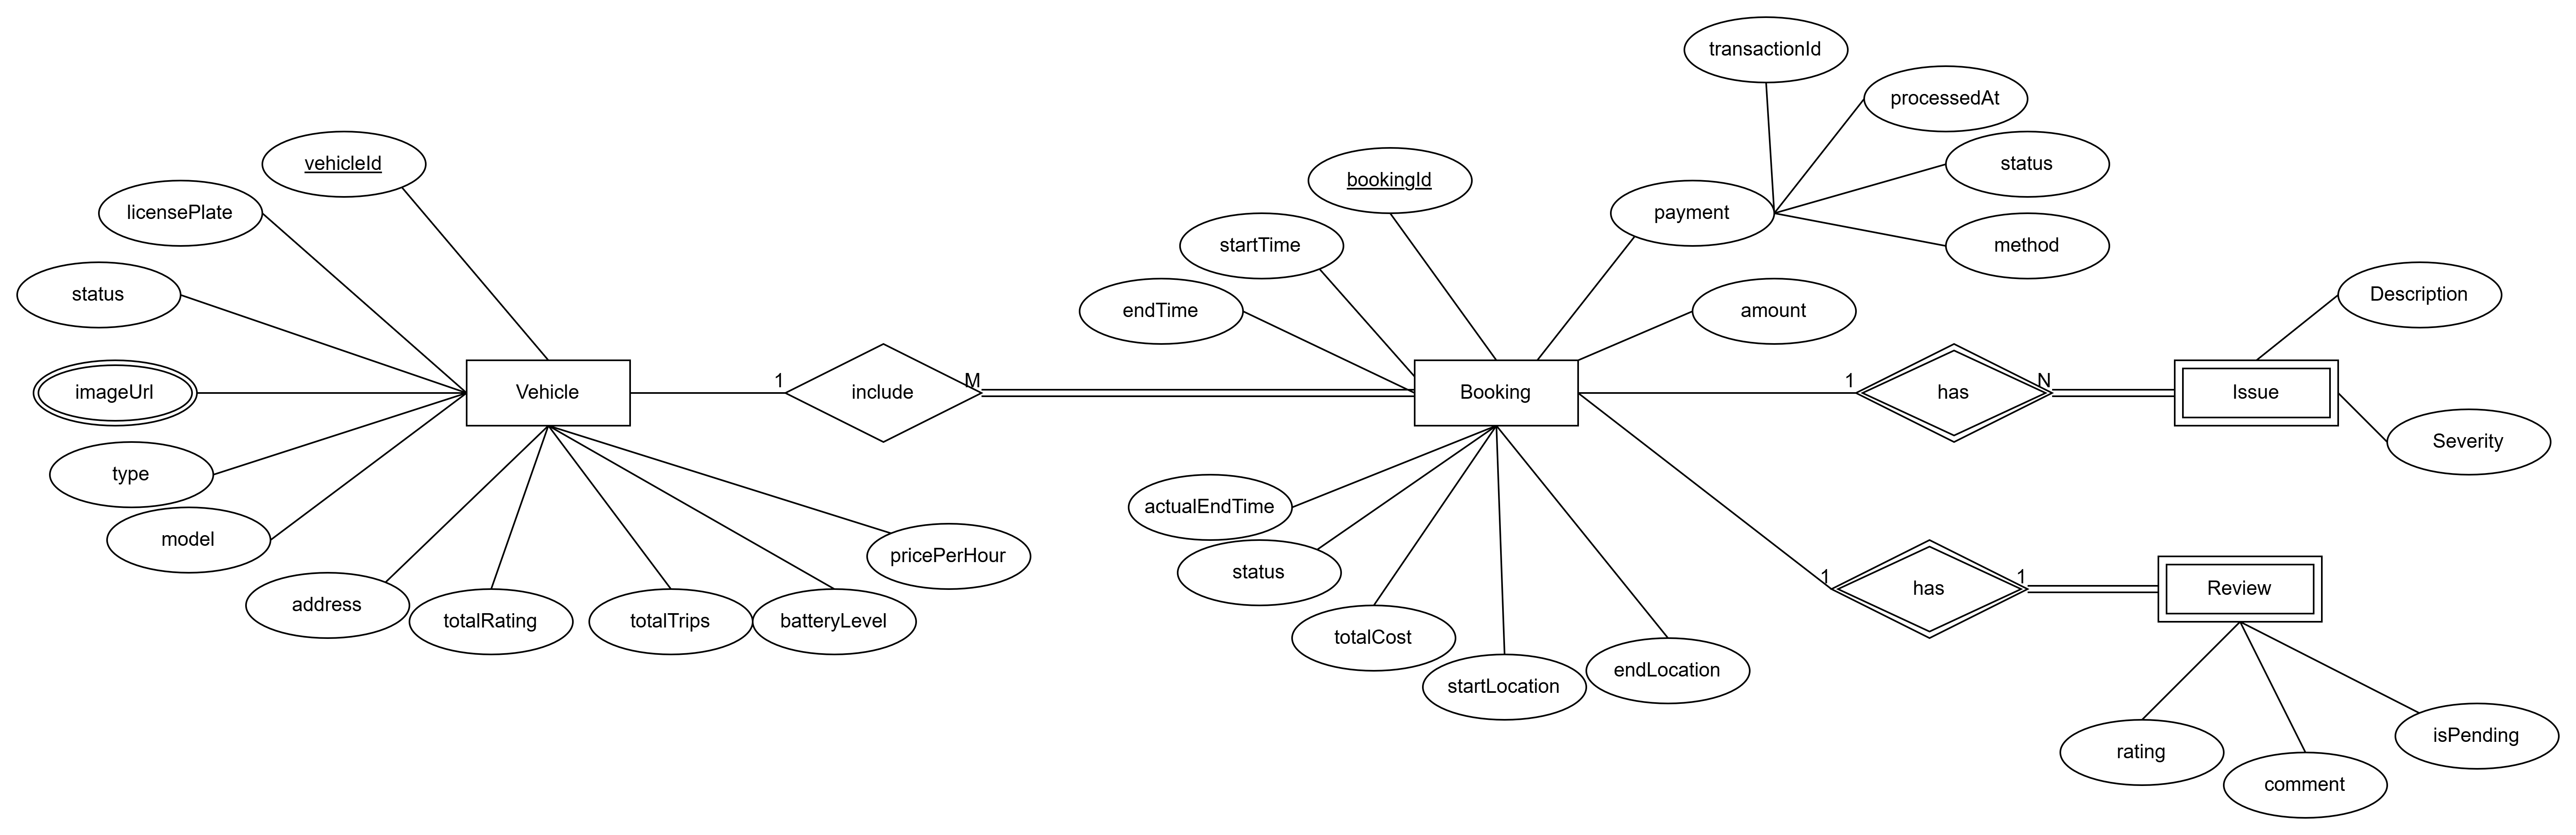
\includegraphics[width=1.0\textwidth]{Images/Design/DB/vehicle-booking.png}
    \caption{Quan hệ giữa \texttt{Vehicle} và \texttt{Booking} (1:N)}
    \label{fig:rel-vehicle-booking}
\end{figure}

\vspace{10pt}

\textbf{(6) Booking} \\[4pt]
\begin{figure}[H]
    \centering
    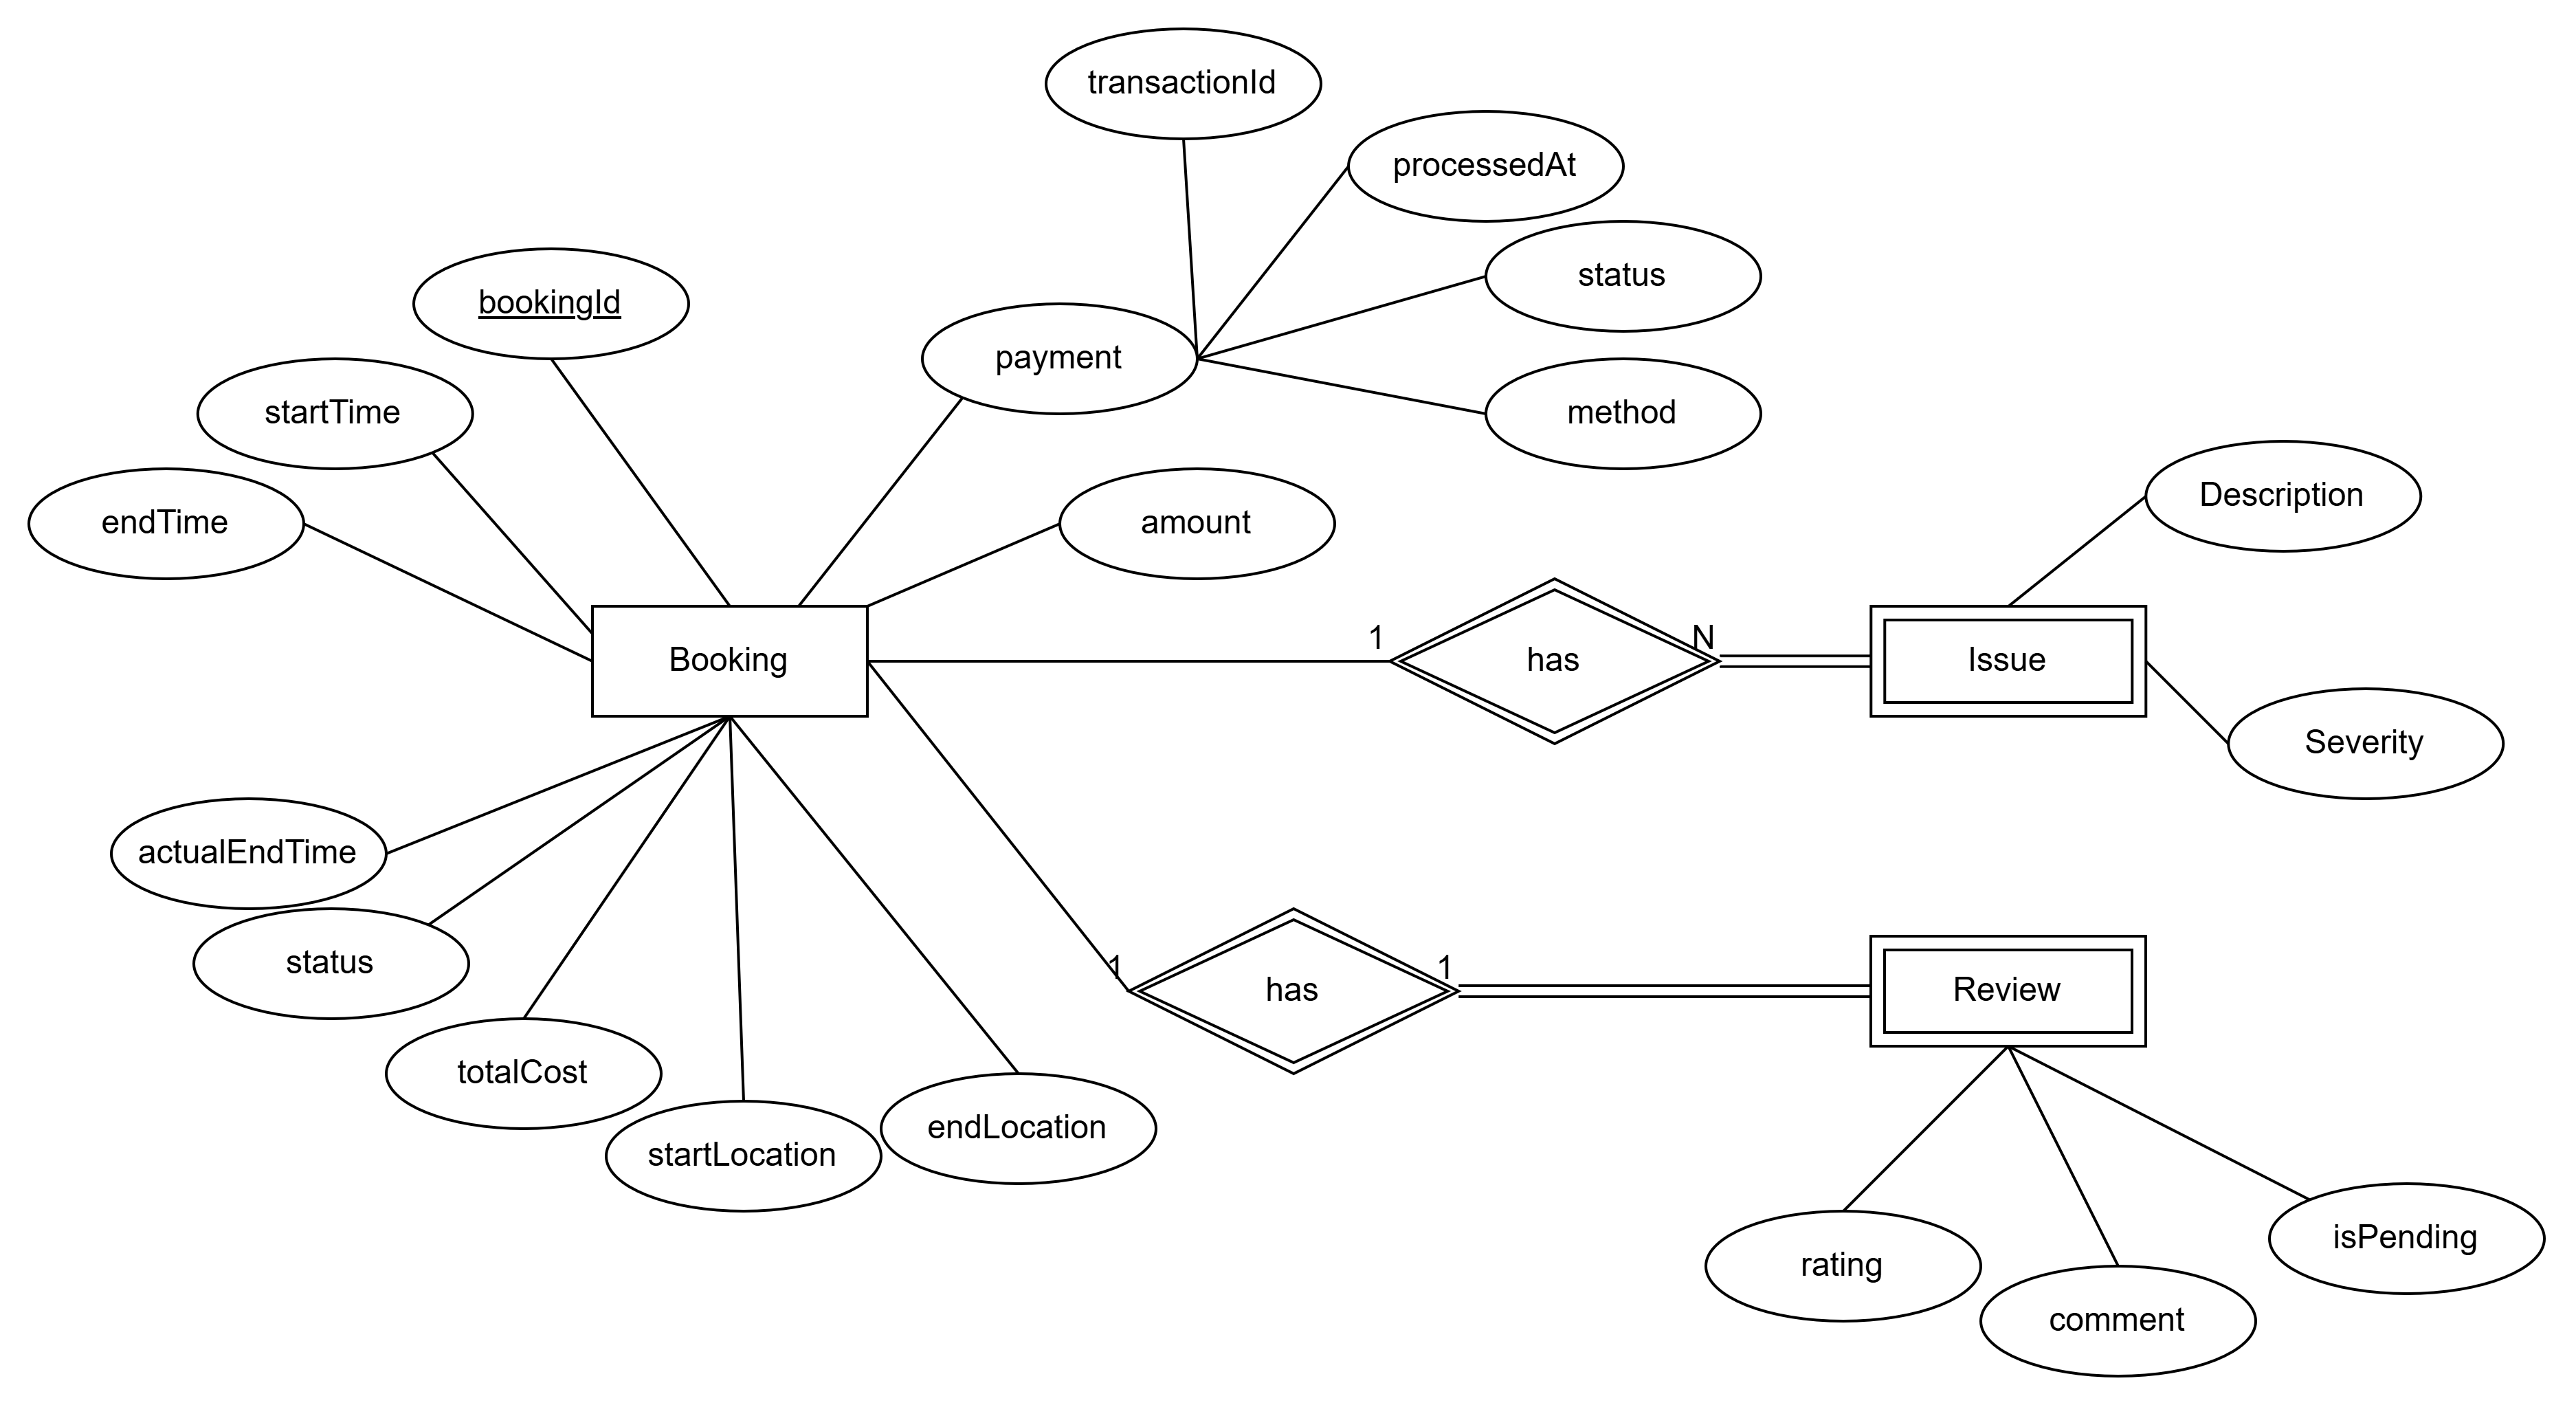
\includegraphics[width=0.8\textwidth]{Images/Design/DB/booking-payment.png}
    \caption{Quan hệ giữa \texttt{Booking} và \texttt{Payment} (1:N)}
    \label{fig:rel-booking-payment}
\end{figure}

\begin{itemize}
    \item[(6.1)] \textbf{Booking -- Review (1:1)} \\[4pt]
    Mỗi \texttt{Review} phải gắn với đúng một \texttt{Booking} (tham gia bắt buộc). 
    Mỗi \texttt{Booking} có đúng một \texttt{Review} (tham gia bắt buộc, quan hệ 1:1). 
    Foreign key \texttt{bookingId} trong bảng \texttt{Review} với constraint NOT NULL và UNIQUE để đảm bảo mỗi booking chỉ có một đánh giá.
    \item[(6.2)] \textbf{Booking -- Issue (1:N)} \\[4pt]
    Một \texttt{Booking} có thể phát sinh nhiều sự cố.  
    Một \texttt{Issue} phải thuộc về đúng một \texttt{Booking}.
\end{itemize}

\textbf{(8) Mối quan hệ kế thừa giữa các thực thể người dùng hệ thống} \\[4pt]
Mỗi \texttt{User} phải thuộc \textbf{đúng 1} trong 3 loại: \texttt{Renter}, \texttt{Owner}, hoặc \texttt{Admin}.
\texttt{Renter}, \texttt{Owner}, \texttt{Admin} chia sẻ \texttt{userId} (FK → User.id)

\begin{figure}[H]
    \centering
    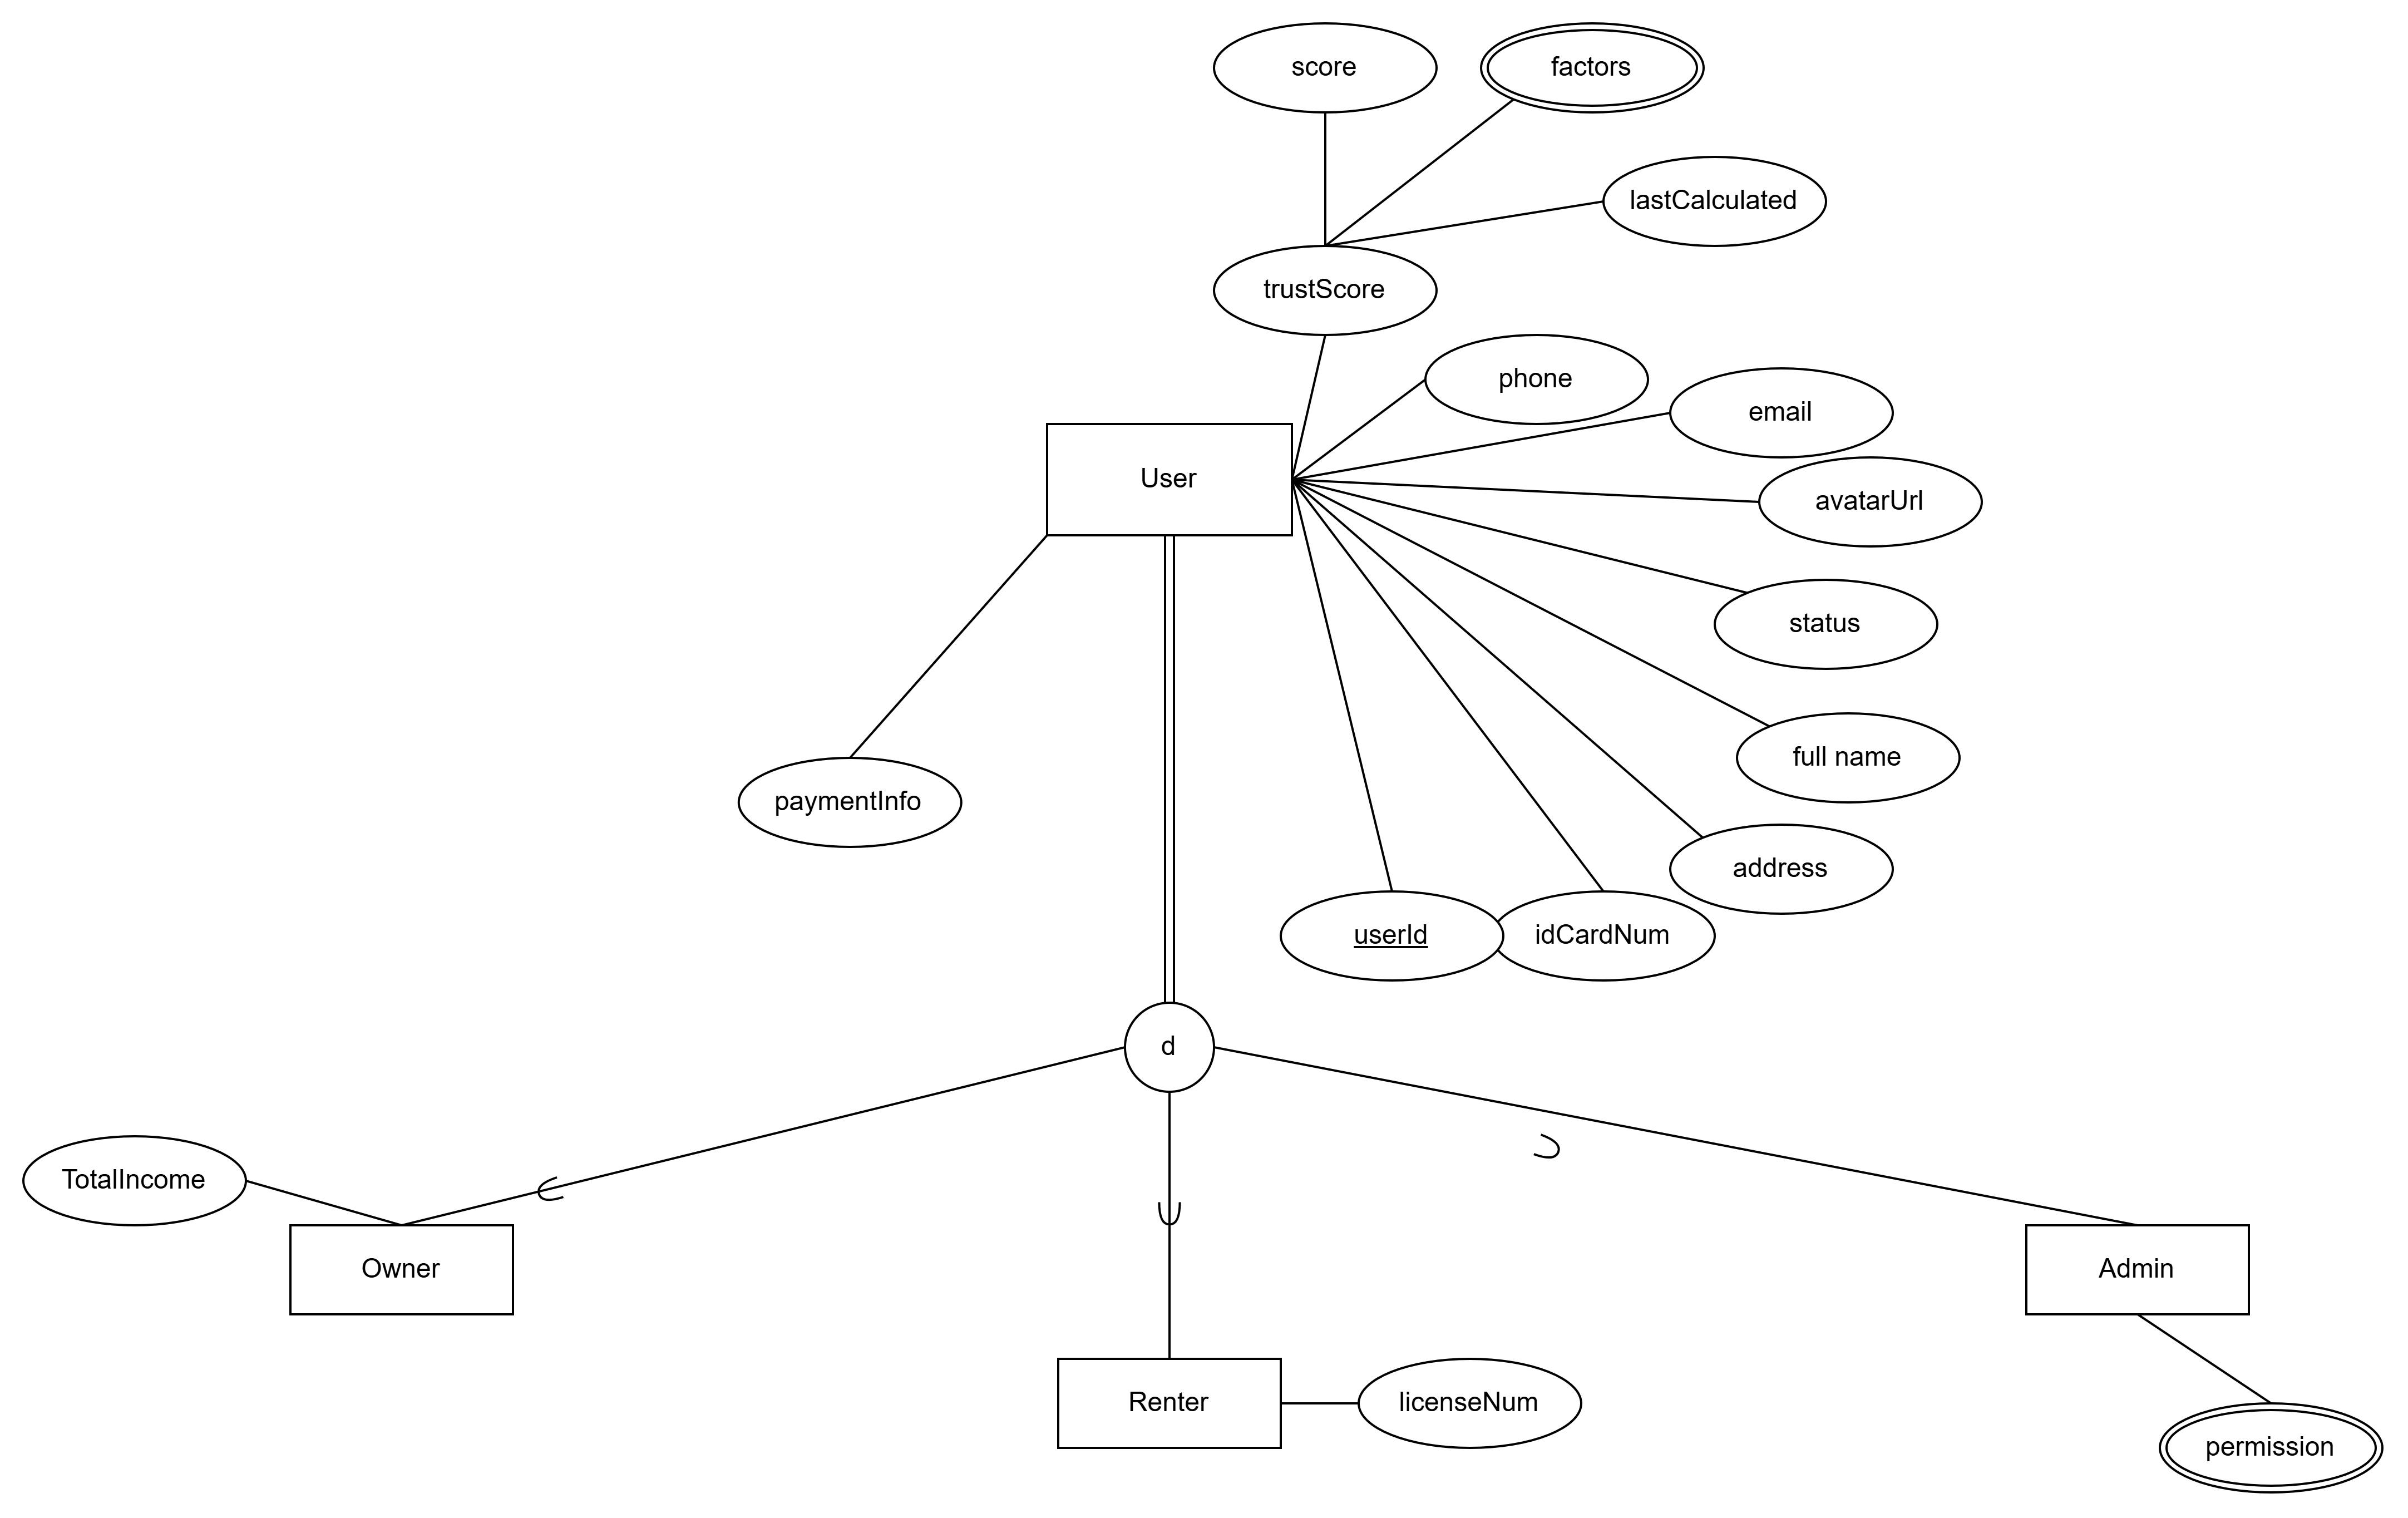
\includegraphics[width=0.8\textwidth]{Images/Design/DB/user.png}
    \caption{Quan hệ kế thừa giữa User với Renter, User, Admin}
    \label{fig:rel-inheritance}
\end{figure}

% \subsubsection*{Kế thừa (Inheritance)}

% Hệ thống sử dụng \textbf{discrete, mandatory inheritance}:
% \begin{itemize}[leftmargin=*]
%     \item Mỗi \texttt{User} phải thuộc \textbf{đúng 1} trong 3 loại: \texttt{Renter}, \texttt{Owner}, hoặc \texttt{Admin}
%     \item Triển khai: Table Per Concrete Class hoặc Single Table Inheritance với trường \texttt{role}
%     \item \texttt{Renter}, \texttt{Owner}, \texttt{Admin} chia sẻ \texttt{userId} (FK → User.id)
% \end{itemize}

% \subsubsection{Ràng buộc toàn vẹn}

% \begin{enumerate}[leftmargin=*]
%     \item \textbf{Notification}: Mỗi notification phải liên kết đến đúng 1 user (NOT NULL \texttt{userId})
%     \item \textbf{Vehicle ownership}: Mỗi vehicle phải có owner (NOT NULL \texttt{ownerId})
%     \item \textbf{Booking}: Mỗi booking phải có renter và vehicle (NOT NULL \texttt{renterId}, \texttt{vehicleId})
%     \item \textbf{Payment}: Mỗi payment phải gắn với 1 booking (NOT NULL \texttt{bookingId})
%     \item \textbf{Review}: Mỗi review phải gắn với 1 booking (NOT NULL \texttt{bookingId}, UNIQUE constraint)
%     \item \textbf{User role}: Mỗi user phải có \texttt{role} $\in$ \{renter, owner, admin\}
%     \item \textbf{Vehicle location}: \texttt{latitude} $\in$ [-90, 90], \texttt{longitude} $\in$ [-180, 180]
%     \item \textbf{Trust score}: \texttt{score} $\in$ [0, 100], \texttt{factors} là JSON array
%     \item \textbf{Booking time}: \texttt{startTime} $ \leqq $ \texttt{endTime}, \texttt{actualEndTime} $\geqq$ \texttt{endTime}
%     \item \textbf{Payment amount}: \texttt{amount} > 0
% \end{enumerate}

% \paragraph{Index và tối ưu hóa}

% \begin{itemize}[leftmargin=*]
%     \item \textbf{Spatial index}: \texttt{CREATE INDEX idx\_vehicle\_location ON vehicles USING GIST (location)}
%     \item \textbf{User queries}: Index trên \texttt{email}, \texttt{phone}, \texttt{status}
%     \item \textbf{Booking queries}: Composite index trên \texttt{(renterId, status)}, \texttt{(vehicleId, startTime)}
%     \item \textbf{Payment queries}: Index trên \texttt{bookingId}, \texttt{status}, \texttt{processedAt}
%     \item \textbf{Full-text search}: Index trên \texttt{Vehicle.model}, \texttt{Vehicle.type}
% \end{itemize}

% \subsection{Yêu cầu dữ liệu}

% \subsubsection{Tổng quan các thực thể dữ liệu}

% Hệ thống chia sẻ xe máy điện P2P quản lý mười thực thể dữ liệu chính, được phân loại thành ba nhóm: dữ liệu chủ (master data) đại diện cho các tham gia viên và tài nguyên hệ thống, dữ liệu giao dịch (transactional data) ghi lại các hoạt động vận hành, và dữ liệu phân tích (analytical data) hỗ trợ giám sát và cải tiến hệ thống.

% \textbf{Dữ liệu chủ} bao gồm User (người tham gia hệ thống với thông tin xác thực và hồ sơ), Renter (chuyên biệt hóa của User với lịch sử thuê và sở thích), Owner (chuyên biệt hóa của User với quyền sở hữu xe và thông tin tài khoản tài chính), Admin (quản trị viên hệ thống với quyền nâng cao), và Vehicle (xe máy điện khả dụng để chia sẻ, bao gồm thông số kỹ thuật và trạng thái hiện tại). Các thực thể này có tần suất cập nhật thấp nhưng tầm quan trọng tham chiếu cao, phục vụ như các mục tiêu khóa ngoại cho các bản ghi giao dịch.

% \textbf{Dữ liệu giao dịch} bao gồm Booking (thỏa thuận thuê xe giữa người thuê và chủ xe, bao gồm khoảng thời gian và tính toán chi phí), Payment (các giao dịch tài chính liên quan đến booking, hỗ trợ nhiều phương thức thanh toán và theo dõi trạng thái), và Review (đánh giá sau khi thuê đóng góp vào tính toán điểm tin cậy). Các thực thể này trải qua khối lượng chèn cao trong quá trình hoạt động hệ thống, tạo thành hồ sơ vận hành cho phép phân tích kinh doanh.

% \textbf{Dữ liệu phân tích và hỗ trợ vận hành} bao gồm Notification (cảnh báo thời gian thực và thông điệp hệ thống cho người dùng) và AnalyticsReport (thống kê tổng hợp được tạo bởi quản trị viên để giám sát hiệu suất hệ thống). Mặc dù không trực tiếp tham gia vào quy trình thuê xe cốt lõi, các thực thể này hỗ trợ trải nghiệm người dùng và các chức năng quản lý hệ thống.

% \subsubsection{Ước tính khối lượng dữ liệu}

% Dự báo khối lượng cung cấp thông tin cho việc lập kế hoạch dung lượng cơ sở dữ liệu và các chiến lược tối ưu hóa truy vấn. Các ước tính xuất phát từ định nghĩa phạm vi dự án: triển khai ban đầu trong 2-3 cộng đồng hỗ trợ khoảng 30-50 xe, 100-150 người dùng hoạt động và 300-500 giao dịch thuê trong giai đoạn thử nghiệm.

% \begin{table}[h]
% \centering
% \caption{Dự báo khối lượng dữ liệu ban đầu (giai đoạn thử nghiệm 6 tháng)}
% \begin{tabular}{|l|r|r|l|}
% \hline
% \textbf{Thực thể} & \textbf{Ban đầu} & \textbf{Tốc độ tăng} & \textbf{Tổng 6 tháng} \\
% \hline
% User & 100 & 10-15/tháng & 150-180 \\
% \hline
% Renter & 80 & 8-12/tháng & 120-150 \\
% \hline
% Owner & 35 & 2-3/tháng & 45-55 \\
% \hline
% Admin & 3 & 0/tháng & 3-5 \\
% \hline
% Vehicle & 40 & 3-5/tháng & 55-65 \\
% \hline
% Booking & 50 & 60-80/tháng & 400-500 \\
% \hline
% Payment & 100 & 120-160/tháng & 800-1,000 \\
% \hline
% Review & 30 & 40-60/tháng & 270-350 \\
% \hline
% Notification & 200 & 300-500/tháng & 2,000-3,200 \\
% \hline
% AnalyticsReport & 0 & 4-8/tháng & 24-48 \\
% \hline
% \end{tabular}
% \end{table}

% Ước tính dung lượng lưu trữ tính đến dữ liệu văn bản, metadata JSON và tham chiếu hình ảnh:

% \begin{itemize}[leftmargin=*]
%     \item \textbf{Thực thể người dùng} (User, Renter, Owner, Admin): Trung bình 2 KB/bản ghi (các trường văn bản, dữ liệu hồ sơ, JSON điểm tin cậy) $\times$ 180 người dùng = 360 KB
%     \item \textbf{Thực thể xe}: Trung bình 5 KB/bản ghi (thông số kỹ thuật, dữ liệu vị trí, tham chiếu hình ảnh) $\times$ 65 xe = 325 KB
%     \item \textbf{Thực thể đặt xe}: Trung bình 1.5 KB/bản ghi (timestamps, tọa độ vị trí, giá) $\times$ 500 bookings = 750 KB
%     \item \textbf{Thực thể thanh toán}: Trung bình 1 KB/bản ghi (dữ liệu giao dịch) $\times$ 1,000 payments = 1 MB
%     \item \textbf{Thực thể đánh giá}: Trung bình 2 KB/bản ghi (xếp hạng, văn bản bình luận) $\times$ 350 reviews = 700 KB
%     \item \textbf{Thực thể thông báo}: Trung bình 0.5 KB/bản ghi (văn bản thông điệp, metadata) $\times$ 3,200 notifications = 1.6 MB
%     \item \textbf{Thực thể báo cáo phân tích}: Trung bình 10 KB/bản ghi (thống kê tổng hợp, tóm tắt JSON) $\times$ 48 reports = 480 KB
% \end{itemize}

% Tổng kích thước cơ sở dữ liệu xấp xỉ 5.2 MB cho dữ liệu có cấu trúc, cộng với khoảng 200-300 MB cho các tệp hình ảnh liên quan (ảnh xe, avatar người dùng). Bao gồm các chỉ mục (ước tính 30\% overhead) và transaction logs, tổng yêu cầu lưu trữ vẫn dưới 1 GB—nằm trong dung lượng của các cơ sở dữ liệu phát triển tiêu chuẩn.

% Đối với các kịch bản mở rộng sản xuất (500 xe, 2,000 người dùng, 10,000 bookings hàng tháng), phép ngoại suy tuyến tính gợi ý tăng trưởng cơ sở dữ liệu lên khoảng 100-150 MB dữ liệu có cấu trúc hàng năm, vẫn có thể quản lý được cho các triển khai PostgreSQL đơn phiên bản hỗ trợ lên đến 100,000 kết nối đồng thời.

% \subsubsection{Yêu cầu chất lượng dữ liệu}

% Các đặc tả chất lượng dữ liệu đảm bảo độ tin cậy hệ thống và niềm tin người dùng thông qua các tiêu chuẩn chính xác, đầy đủ, nhất quán và kịp thời rõ ràng:

% \textbf{Yêu cầu về độ chính xác.} Dữ liệu không gian địa lý phải đạt độ chính xác GPS trong vòng ±10 mét đối với tọa độ vị trí xe để cho phép tìm kiếm gần đáng tin cậy. Các giao thức thử nghiệm xác minh độ chính xác vị trí so với các vị trí ground truth được đo bằng thiết bị GPS cấp khảo sát. Báo cáo mức pin yêu cầu độ chính xác ±5\%, được xác thực thông qua tương quan với các số đọc hệ thống quản lý pin (BMS) thực tế khi có sẵn. Các tính toán tài chính phải đạt độ chính xác thập phân chính xác để ngăn chặn lỗi làm tròn trong các tình huống đa tiền tệ hoặc thanh toán phân số.

% \textbf{Yêu cầu về tính đầy đủ.} Các thực thể cốt lõi thực thi các ràng buộc trường bắt buộc để ngăn chặn các bản ghi không đầy đủ làm giảm chức năng hệ thống:

% \begin{table}[h]
% \centering
% \caption{Yêu cầu trường bắt buộc theo thực thể}
% \small
% \begin{tabular}{|p{3cm}|p{11cm}|}
% \hline
% \textbf{Thực thể} & \textbf{Các trường bắt buộc} \\
% \hline
% User & fullName, email, phone, role, status, createdAt \\
% \hline
% Vehicle & licensePlate, ownerId, status, type, batteryLevel, pricePerHour, location (lat/lng) \\
% \hline
% Booking & renterId, vehicleId, startTime, endTime, status, totalCost \\
% \hline
% Payment & bookingId, amount, method, status, processedAt \\
% \hline
% Review & bookingId, rating (1-5), createdAt \\
% \hline
% \end{tabular}
% \end{table}

% Việc thực thi schema cơ sở dữ liệu thông qua các ràng buộc NOT NULL ngăn chặn việc chèn bản ghi không đầy đủ. Xác thực tầng ứng dụng cung cấp phản hồi người dùng ngay lập tức khi các trường bắt buộc vẫn chưa được điền, cải thiện chất lượng thu thập dữ liệu tại nguồn.

% \textbf{Yêu cầu về tính nhất quán.} Các ràng buộc toàn vẹn tham chiếu duy trì các mối quan hệ logic giữa các thực thể: bookings tham chiếu đến xe và người thuê hợp lệ thông qua các ràng buộc khóa ngoại với chính sách xóa CASCADE để ngăn chặn các bản ghi mồ côi. Các giá trị trường trạng thái xuất phát từ các bảng liệt kê được xác định trước (ví dụ: Vehicle.status $\in$ \{available, rented, maintenance, inactive\}) được thực thi thông qua các ràng buộc CHECK cơ sở dữ liệu và xác thực tầng ứng dụng.

% Các quy tắc nhất quán giữa các thực thể bao gồm: (1) một xe không thể có các bookings chồng chéo ở trạng thái 'active', được thực thi thông qua các chỉ mục một phần duy nhất trên (vehicleId, status) WHERE status = 'active'; (2) số tiền thanh toán phải khớp với tính toán totalCost của booking trong dung sai chấp nhận được (±0.01), được xác minh thông qua các hàm trigger hoặc các assertion tầng ứng dụng; (3) xếp hạng đánh giá đóng góp vào xếp hạng tổng hợp xe và chủ xe, được duy trì thông qua trigger cơ sở dữ liệu hoặc cập nhật theo lô theo lịch trình.

% \textbf{Yêu cầu về tính kịp thời.} Các đặc tả độ tươi dữ liệu thay đổi theo loại thực thể và mẫu sử dụng:

% \begin{itemize}[leftmargin=*]
%     \item \textbf{Vị trí xe}: Cập nhật mỗi 10 giây trong các chuyến thuê hoạt động, được đệm thông qua bộ nhớ cache Redis để giảm tải ghi cơ sở dữ liệu. Dữ liệu vị trí cũ vượt quá 60 giây kích hoạt cảnh báo "vị trí không khả dụng" trong UI.
%     \item \textbf{Tính khả dụng xe}: Cập nhật thời gian thực khi có thay đổi trạng thái booking. Thông báo WebSocket đảm bảo UI phản ánh tính khả dụng trong vòng 2 giây sau các chuyển đổi trạng thái.
%     \item \textbf{Mức pin}: Cập nhật mỗi 30 giây trong các chuyến thuê hoạt động, hoặc theo yêu cầu khi người dùng yêu cầu chi tiết xe.
%     \item \textbf{Điểm tin cậy}: Được tính toán lại bất đồng bộ trong vòng 5 phút sau khi gửi đánh giá mới, cân bằng khả năng phản hồi với hiệu quả tính toán.
%     \item \textbf{Báo cáo phân tích}: Được tạo theo yêu cầu hoặc qua các công việc theo lịch trình (hàng ngày/hàng tuần), với độ cũ chấp nhận được lên đến 24 giờ cho số liệu thống kê tóm tắt.
% \end{itemize}

% \subsubsection{Bảo mật và quyền riêng tư dữ liệu}

% Các đặc tả bảo mật và quyền riêng tư phù hợp với các nguyên tắc GDPR (mặc dù bối cảnh bảo vệ dữ liệu của Việt Nam đang phát triển) để thiết lập các thực hành có thể bảo vệ được:

% \textbf{Phân loại Thông tin Nhận dạng Cá nhân (PII).} Các yếu tố dữ liệu được phân loại thành các cấp độ nhạy cảm:

% \begin{itemize}[leftmargin=*]
%     \item \textbf{Độ nhạy cao}: Thông tin xác thực (password hashes), chi tiết tài khoản tài chính (bankAccount), số nhận dạng (idCardNum, licenseNum), lịch sử vị trí chính xác. Các trường này yêu cầu mã hóa khi lưu trữ và truyền tải, với quyền truy cập hạn chế chỉ cho các quy trình được ủy quyền.
%     \item \textbf{Độ nhạy trung bình}: Thông tin liên lạc (email, phone), tên, hồ sơ sở hữu xe. Được bảo vệ thông qua kiểm soát truy cập nhưng không được mã hóa trong cơ sở dữ liệu (để cho phép tìm kiếm hiệu quả).
%     \item \textbf{Độ nhạy thấp}: Thống kê tổng hợp, mẫu sử dụng ẩn danh, thông số kỹ thuật xe. Phù hợp cho phân tích mà không cần bảo vệ bổ sung.
% \end{itemize}

% \textbf{Đặc tả mã hóa.} Dữ liệu nhạy cảm sử dụng nhiều lớp bảo vệ: (1) Transport Layer Security (TLS 1.3) mã hóa tất cả các giao tiếp client-server; (2) Lưu trữ mật khẩu sử dụng băm bcrypt với hệ số chi phí 12, ngăn chặn các cuộc tấn công bảng rainbow; (3) Mã hóa cấp cột cơ sở dữ liệu (sử dụng phần mở rộng pgcrypto của PostgreSQL) bảo vệ chi tiết tài khoản tài chính và số nhận dạng; (4) API tokens sử dụng JWT với chữ ký RS256 và hết hạn 24 giờ, giảm thiểu rủi ro thỏa hiệp token.

% \textbf{Ma trận kiểm soát truy cập.} Kiểm soát truy cập dựa trên vai trò (RBAC) hạn chế khả năng hiển thị dữ liệu:

% \begin{table}[h]
% \centering
% \caption{Quyền truy cập dữ liệu theo vai trò}
% \small
% \begin{tabular}{|p{3.5cm}|p{3cm}|p{3cm}|p{3cm}|}
% \hline
% \textbf{Thực thể dữ liệu} & \textbf{Renter} & \textbf{Owner} & \textbf{Admin} \\
% \hline
% Hồ sơ User riêng & Đọc, Cập nhật & Đọc, Cập nhật & Đọc, Cập nhật \\
% \hline
% Hồ sơ User khác & Đọc (hạn chế) & Đọc (hạn chế) & Đọc, Cập nhật, Xóa \\
% \hline
% Bookings riêng & Đọc, Tạo, Hủy & Đọc & Đọc, Cập nhật \\
% \hline
% Bookings khác & Không & Đọc (xe riêng) & Đọc, Cập nhật \\
% \hline
% Vehicles & Đọc (tất cả), Đặt & Đọc, Tạo, Cập nhật & Đọc, Cập nhật, Xóa \\
% \hline
% Payments & Đọc (riêng) & Đọc (riêng) & Đọc (tất cả) \\
% \hline
% Reviews & Tạo (riêng) & Đọc (xe riêng) & Đọc, Cập nhật, Xóa \\
% \hline
% \end{tabular}
% \end{table}

% \textbf{Chính sách lưu giữ dữ liệu.} Các lịch trình lưu giữ cân bằng nhu cầu vận hành với các nguyên tắc quyền riêng tư: (1) Tài khoản người dùng hoạt động và dữ liệu liên quan tồn tại vô thời hạn trong khi tài khoản vẫn hoạt động; (2) Tài khoản không hoạt động (không đăng nhập trong 24 tháng) kích hoạt lưu trữ dữ liệu với ẩn danh hóa PII sau khi thông báo người dùng; (3) Hồ sơ booking và payment lưu giữ trong 36 tháng để hỗ trợ tuân thủ thuế và giải quyết tranh chấp, sau đó lưu trữ với sửa đổi PII; (4) Lịch sử vị trí tổng hợp thành tóm tắt hàng ngày sau 90 ngày, với tọa độ chính xác bị loại bỏ; (5) Thông báo hết hạn sau 30 ngày trừ khi được đánh dấu để lưu giữ bởi người dùng.

% \subsubsection{Yêu cầu tích hợp dữ liệu}

% Hệ thống tích hợp các nguồn dữ liệu bên ngoài và đồng bộ hóa trên các thành phần phân tán:

% \textbf{Nguồn dữ liệu bên ngoài.} Các tích hợp bên thứ ba đưa ra yêu cầu luồng dữ liệu:

% \begin{itemize}[leftmargin=*]
%     \item \textbf{API bản đồ} (Google Maps Platform): Geocoding cho chuyển đổi địa chỉ-sang-tọa độ, reverse geocoding cho hiển thị tọa độ-sang-địa chỉ, và tính toán tuyến đường để ước tính khoảng cách. Các phản hồi API cache trong 24 giờ để giảm thiểu tiêu thụ quota và cải thiện độ trễ phản hồi.
%     \item \textbf{Cổng thanh toán} (VNPay, Momo): Cập nhật trạng thái giao dịch đến qua webhook callbacks yêu cầu xử lý idempotent (ID giao dịch trùng lặp bị từ chối). Dữ liệu xác nhận thanh toán xác thực so với hồ sơ booking nội bộ trước khi đánh dấu giao dịch hoàn tất.
%     \item \textbf{Dịch vụ AI/ML} (tương lai): Công cụ khuyến nghị tiêu thụ các mẫu sử dụng ẩn danh (thời gian booking, vị trí, thời lượng) để tạo các đề xuất thời gian thuê. Xuất dữ liệu qua các công việc ETL theo lịch trình (hàng đêm) vào kho dữ liệu phân tích.
% \end{itemize}

% \textbf{Đồng bộ hóa di động-server.} Tính nhất quán dữ liệu client-server sử dụng nhiều chiến lược:

% \begin{itemize}[leftmargin=*]
%     \item \textbf{Cập nhật lạc quan}: UI client ngay lập tức phản ánh các hành động người dùng (yêu cầu booking, cập nhật hồ sơ) với các cuộc gọi API nền. Từ chối server kích hoạt rollback với thông báo người dùng.
%     \item \textbf{Đồng bộ hóa delta}: Dữ liệu thường xuyên (vị trí xe) chỉ truyền các thay đổi kể từ lần cập nhật cuối cùng, giảm 60-70\% tiêu thụ băng thông so với các chuyển trạng thái đầy đủ.
%     \item \textbf{Giải quyết xung đột}: Cập nhật đồng thời đối với tài nguyên chia sẻ (booking xe) giải quyết thông qua last-write-wins với so sánh timestamp booking. Các yêu cầu booking sớm hơn nhận được ưu tiên khi xung đột xảy ra trong cửa sổ 5 giây.
% \end{itemize}

% \textbf{Xử lý dữ liệu ngoại tuyến.} Các ứng dụng di động duy trì bộ nhớ cache local để hỗ trợ chức năng ngoại tuyến hạn chế:

% \begin{itemize}[leftmargin=*]
%     \item \textbf{Thao tác đọc}: Xe đã xem gần đây, lịch sử booking và hồ sơ người dùng cache local (lưu trữ SQLite) để xem ngoại tuyến. Độ cũ dữ liệu được chỉ ra thông qua timestamps UI.
%     \item \textbf{Thao tác ghi}: Yêu cầu booking ngoại tuyến xếp hàng local với thử lại định kỳ. Người dùng nhận cảnh báo về chức năng ngoại tuyến hạn chế cho các hoạt động giao dịch.
%     \item \textbf{Đồng bộ hóa}: Chuyển đổi foreground app kích hoạt đồng bộ hóa nền, tải lên các hoạt động đã xếp hàng và fetch các thay đổi phía server.
% \end{itemize}
\subsection{Thiết kế giao diện người dùng}

Giao diện người dùng được thiết kế và triển khai hoàn toàn bằng Flutter với BLoC pattern, tuân thủ Material 3 Design, tối ưu cho thiết bị di động (iOS \& Android).

Các màn hình được prototype trên Figma (xem phụ lục C).

\subsubsection{Onboarding}

\begin{figure}[H]
    \centering
    \begin{subfigure}[b]{0.32\textwidth}
        \centering
        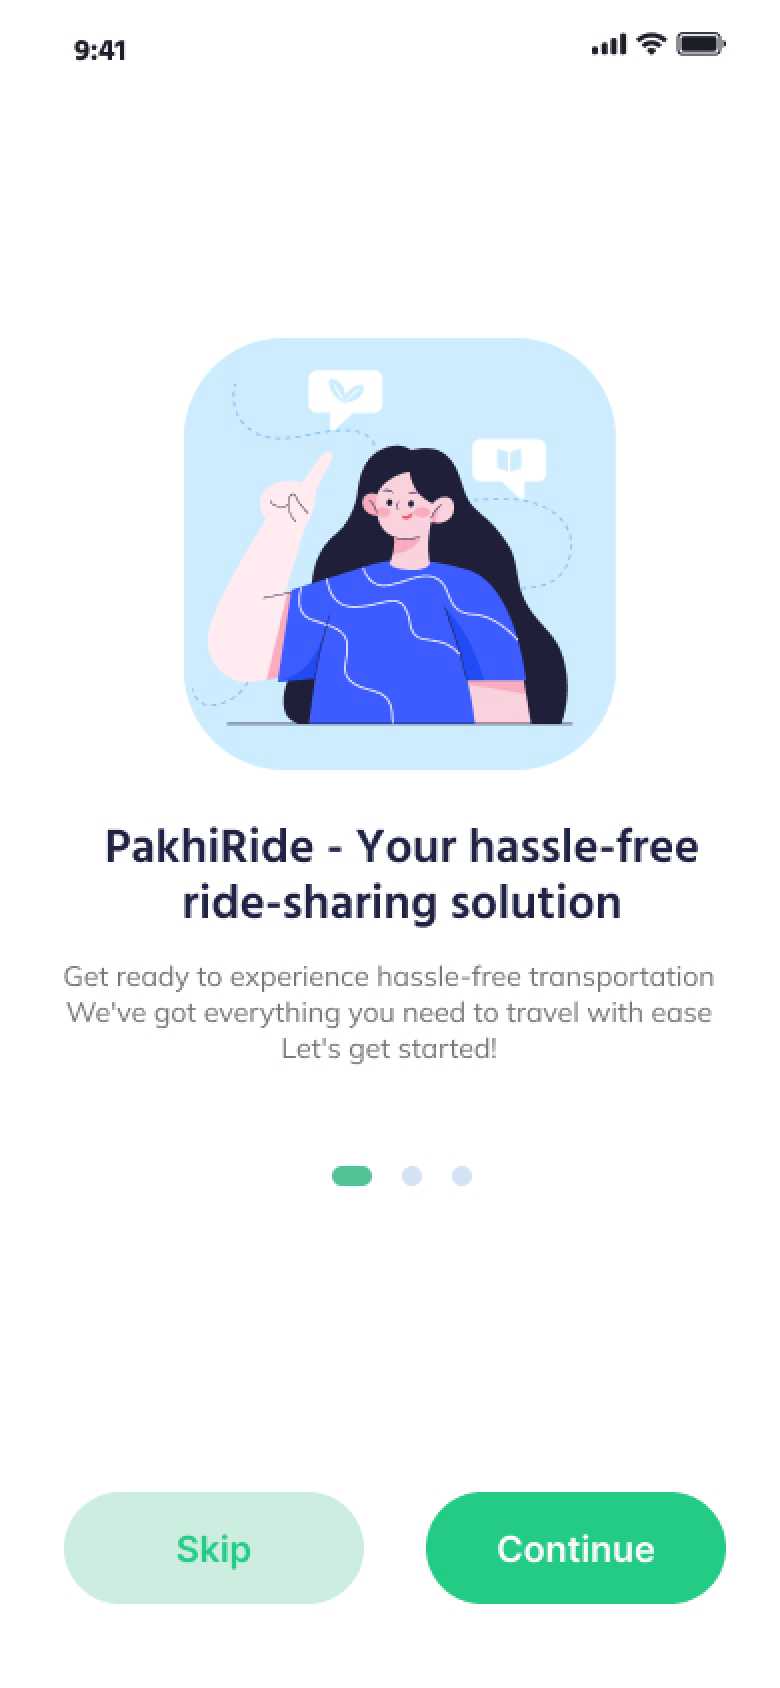
\includegraphics[width=\textwidth]{Images/Design/UIUX/onboard/ob1.png}
        \caption{Onboarding 1}
    \end{subfigure}
    \hfill
    \begin{subfigure}[b]{0.32\textwidth}
        \centering
        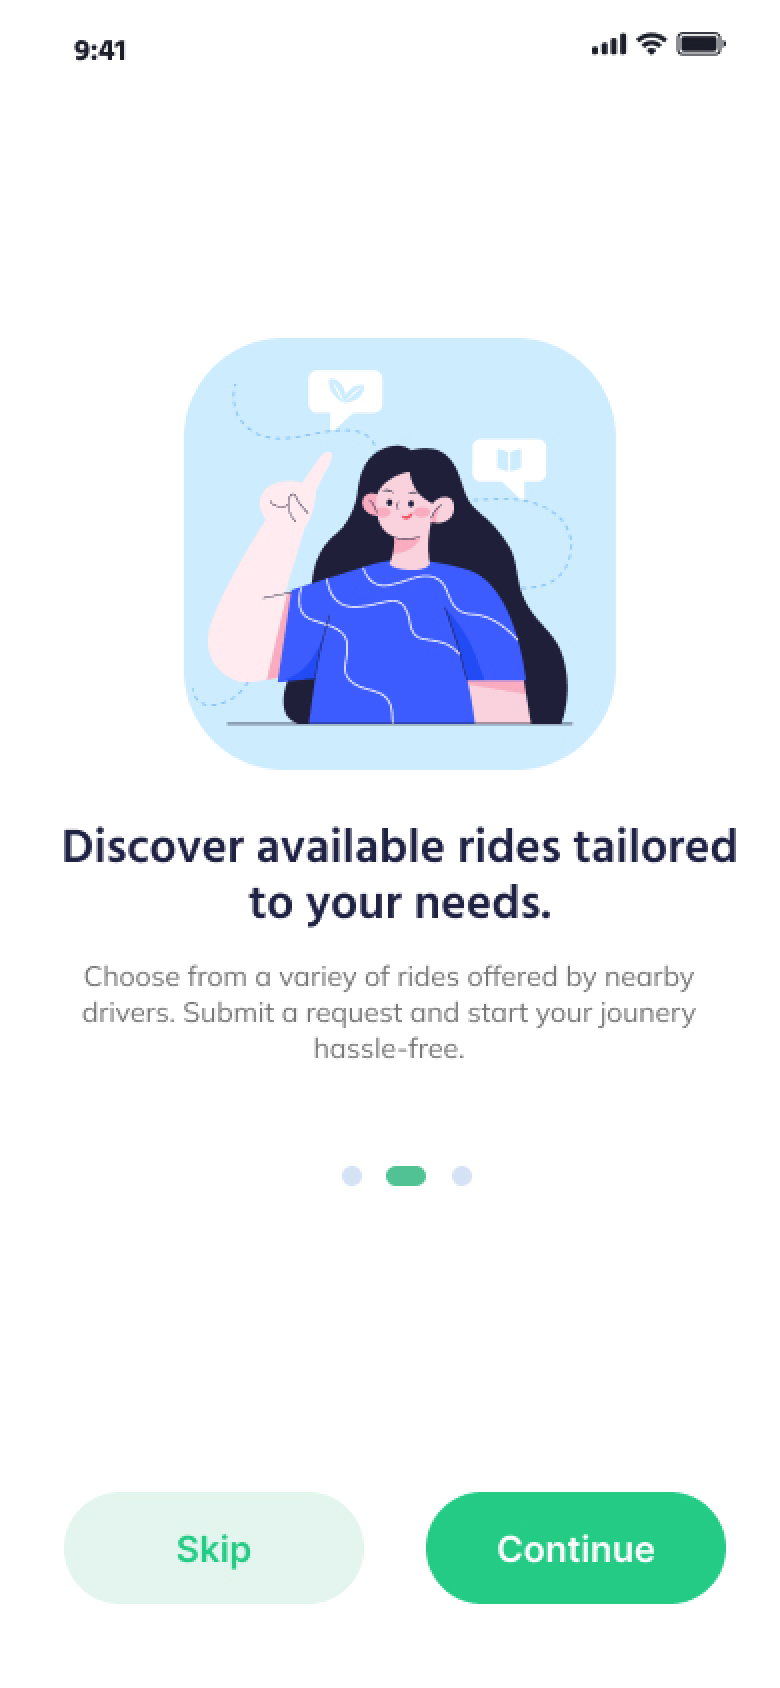
\includegraphics[width=\textwidth]{Images/Design/UIUX/onboard/ob2.png}
        \caption{Onboarding 2}
    \end{subfigure}
    \hfill
    \begin{subfigure}[b]{0.32\textwidth}
        \centering
        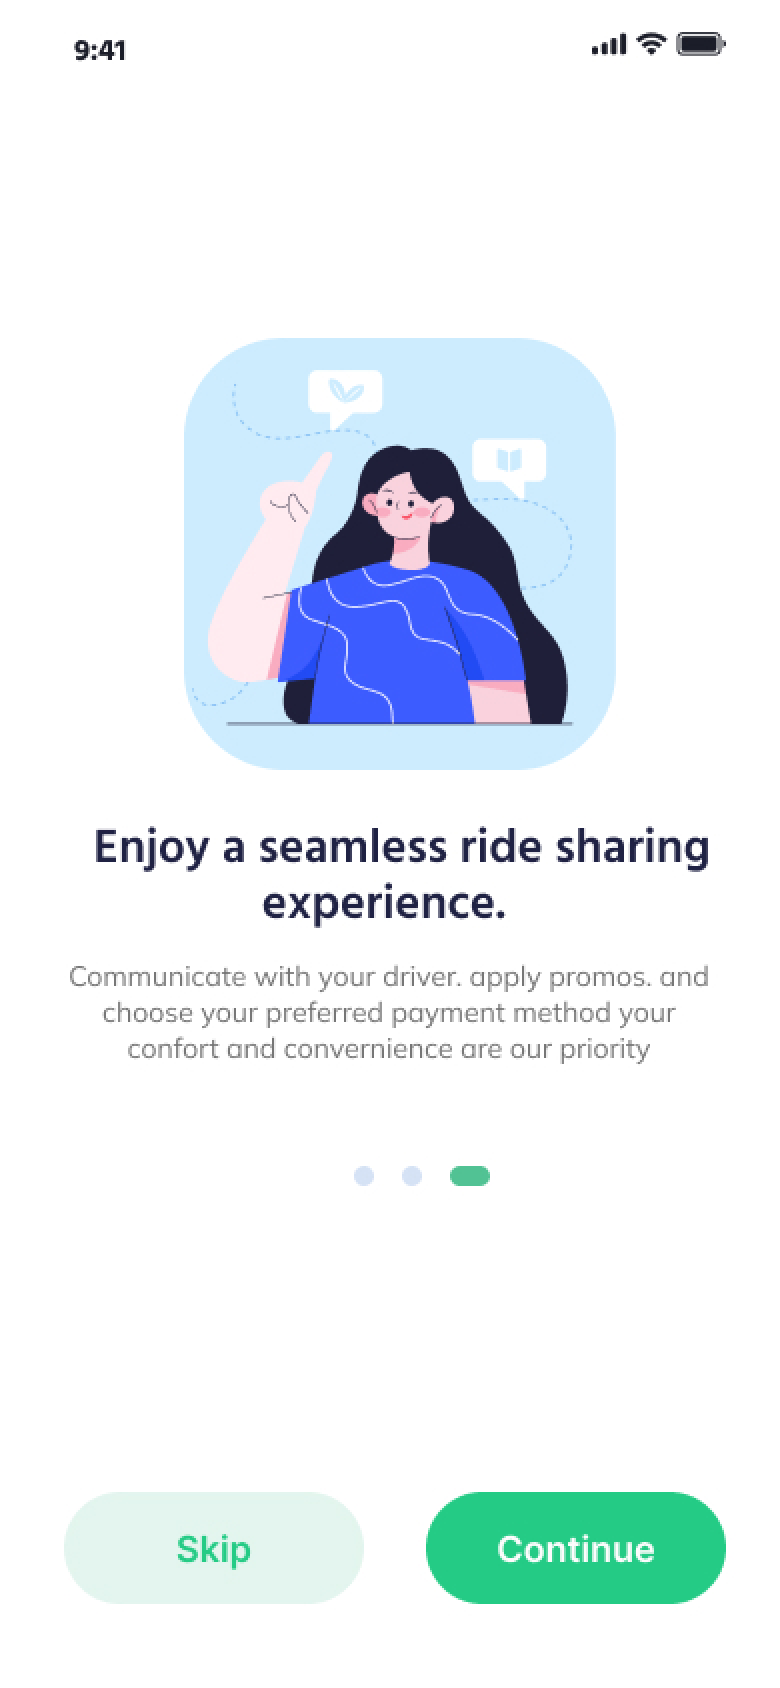
\includegraphics[width=\textwidth]{Images/Design/UIUX/onboard/ob3.png}
        \caption{Onboarding 3}
    \end{subfigure}
    \caption{Giao diện khởi tạo tài khoản (UC-01)}
    \label{fig:ui-onboard}
\end{figure}
Màn hình onboarding giới thiệu ngắn gọn mô hình chia sẻ P2P và lợi ích môi trường. 

\newpage
\subsubsection{Đăng nhập – Đăng ký}
\begin{figure}[H]
    \centering
    \begin{subfigure}[b]{0.32\textwidth}
        \centering
        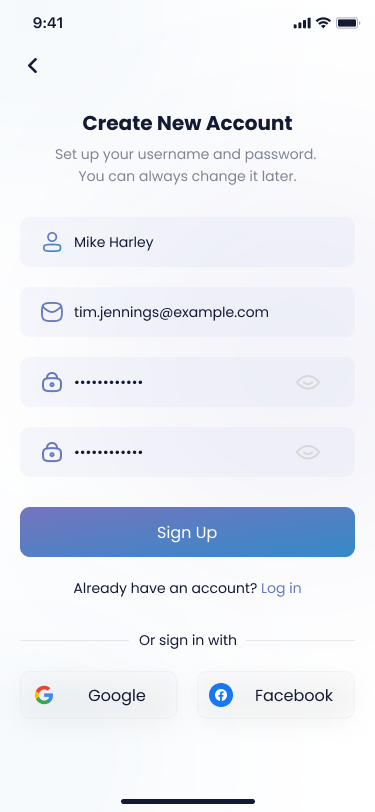
\includegraphics[width=\textwidth]{Images/Design/UIUX/auth/regis.png}
        \caption{Đăng ký}
    \end{subfigure}
    \hfill
    \begin{subfigure}[b]{0.32\textwidth}
        \centering
        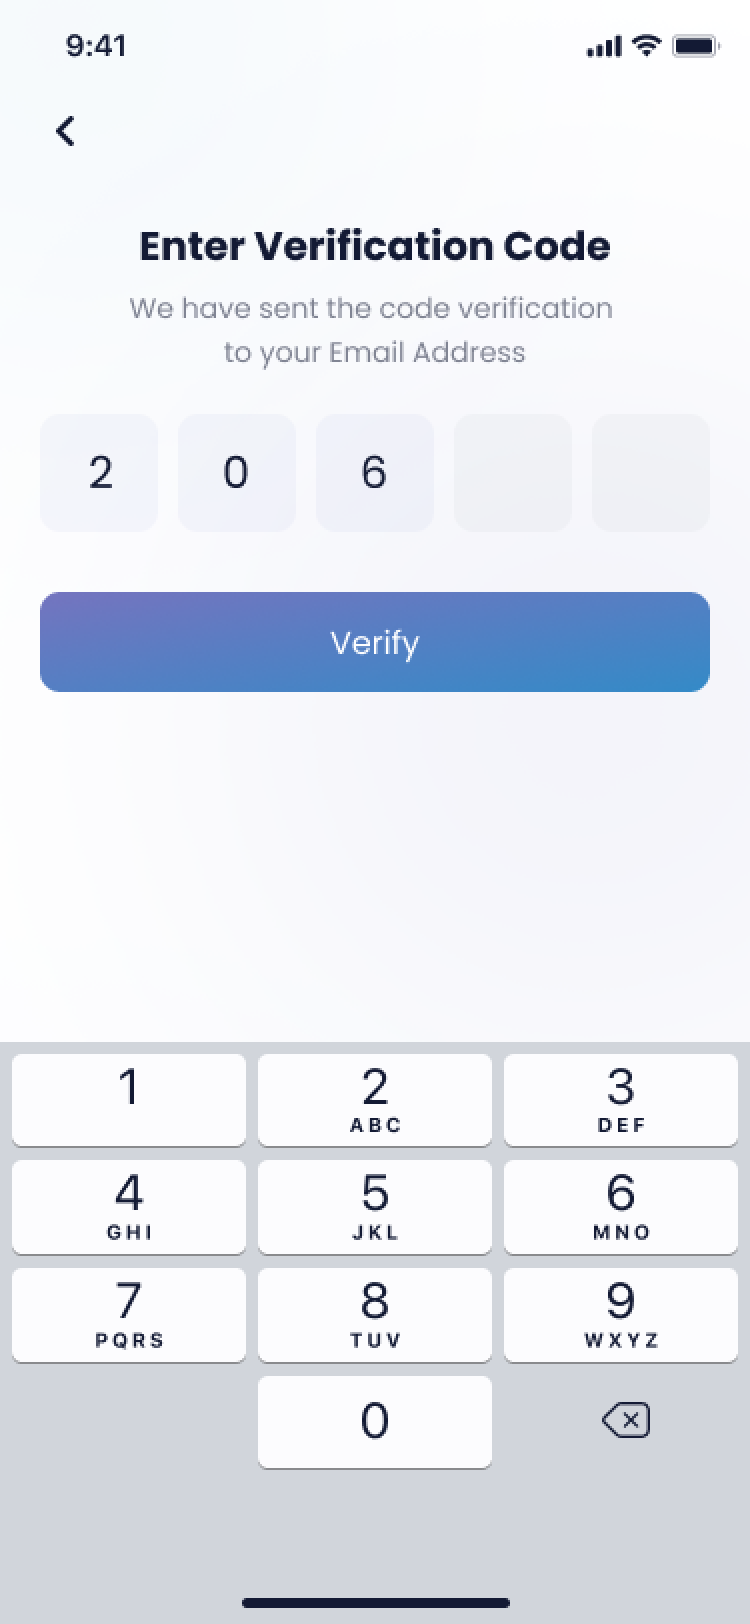
\includegraphics[width=\textwidth]{Images/Design/UIUX/auth/otp.png}
        \caption{OTP}
    \end{subfigure}
    \hfill
    \begin{subfigure}[b]{0.32\textwidth}
        \centering
        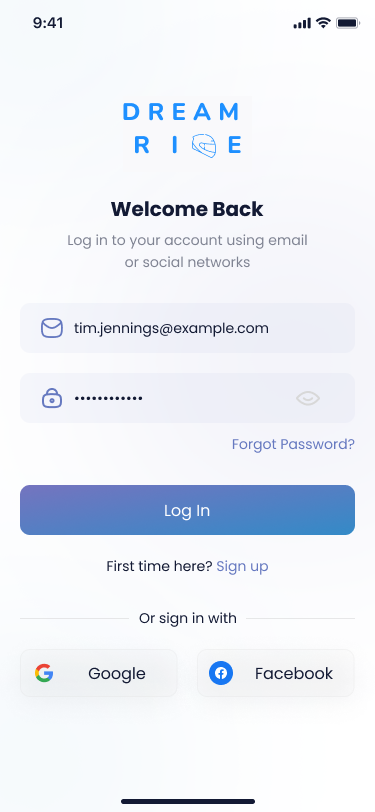
\includegraphics[width=\textwidth]{Images/Design/UIUX/auth/login.png}
        \caption{Đăng nhập}
    \end{subfigure}
    \caption{Giao diện khởi tạo tài khoản (UC-01)}
    \label{fig:ui-auth}
\end{figure}
Người dùng có thể đăng nhập nhanh bằng email/số điện thoại + OTP hoặc OAuth (Google/Zalo). Quy trình đăng ký yêu cầu xác minh CCCD và selfie để đảm bảo tính xác thực ngay từ đầu — yếu tố then chốt xây dựng niềm tin trong hệ thống chia sẻ ngang hàng. Giao diện tối giản, chỉ hiển thị một hành động chính tại một thời điểm, giảm tỷ lệ thoát người dùng mới.
\newpage

\subsubsection{Trang chủ \& Tìm kiếm xe}

\begin{figure}[H]
    \centering
    \begin{subfigure}[b]{0.32\textwidth}
        \centering
        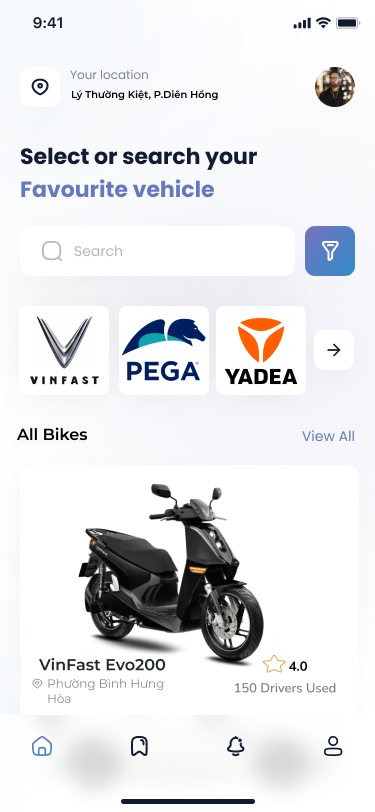
\includegraphics[width=\textwidth]{Images/Design/UIUX/Home/home.png}
        \caption{Home screen}
    \end{subfigure}
    \hfill
    \begin{subfigure}[b]{0.32\textwidth}
        \centering
        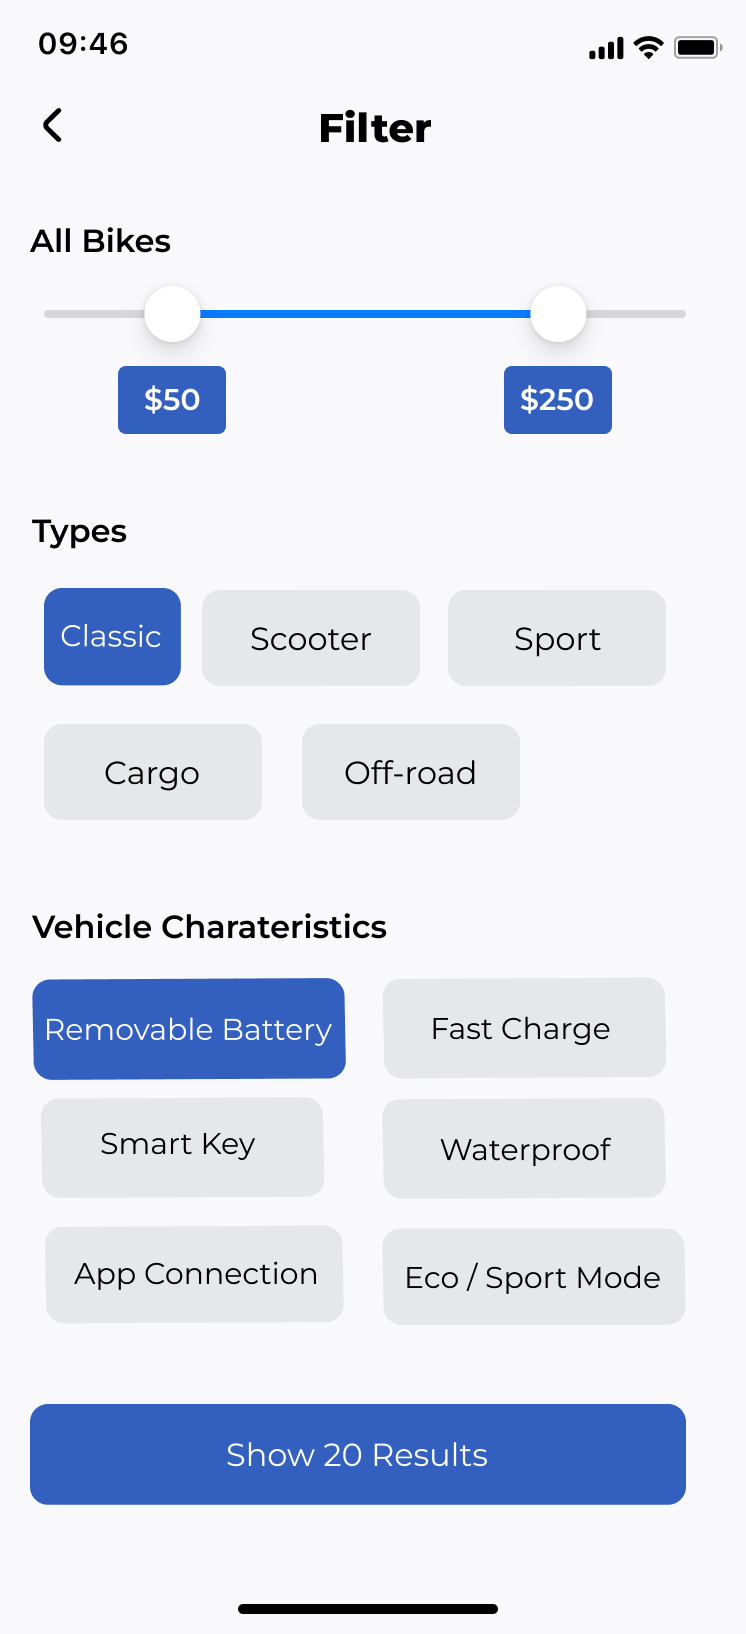
\includegraphics[width=\textwidth]{Images/Design/UIUX/Home/filter.png}
        \caption{Bộ lọc tìm kiếm}
    \end{subfigure}
    \hfill
    \begin{subfigure}[b]{0.32\textwidth}
        \centering
        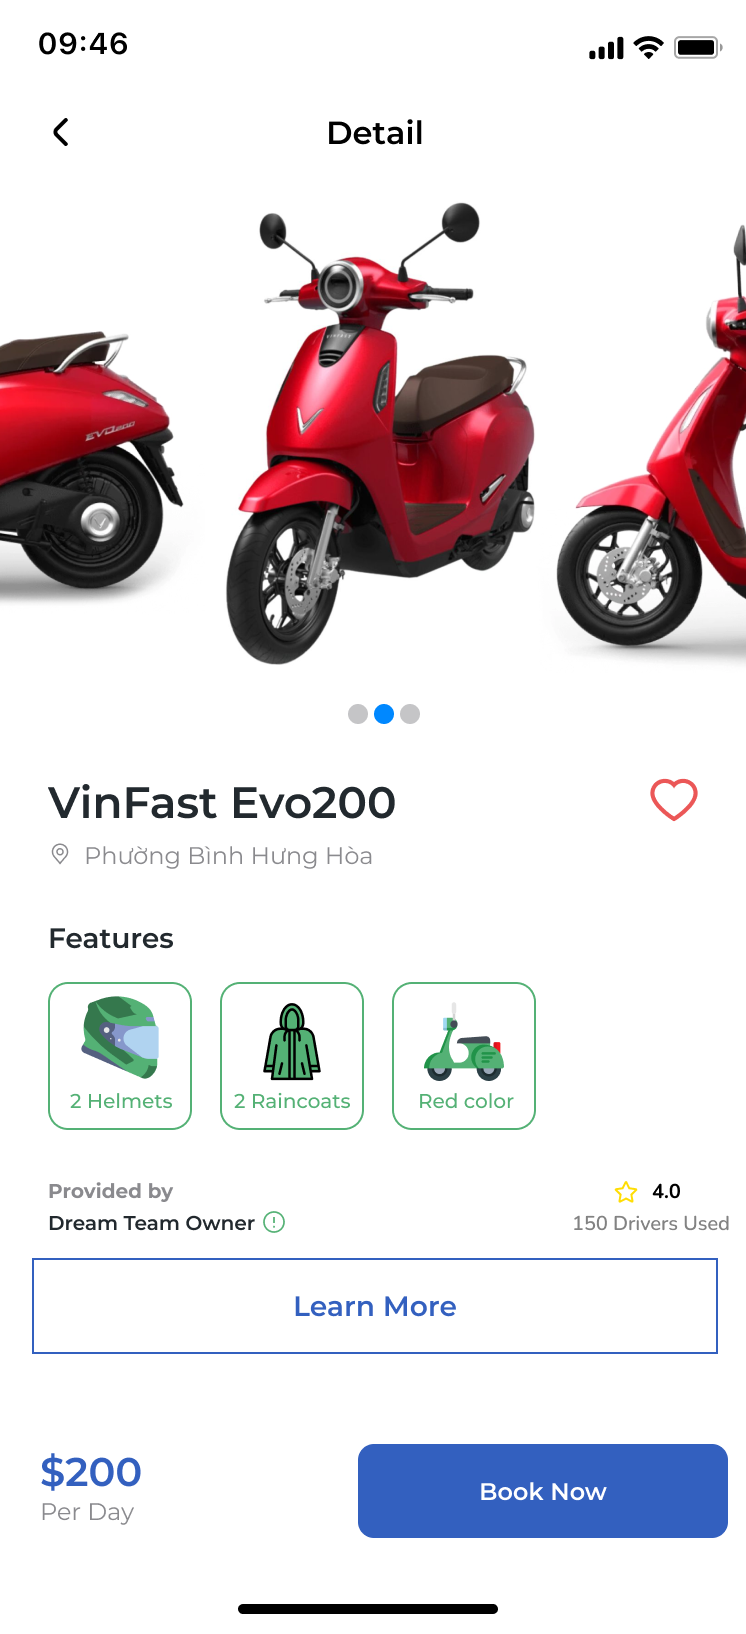
\includegraphics[width=\textwidth]{Images/Design/UIUX/Home/details.png}
        \caption{Chi tiết xe}
    \end{subfigure}
    \caption{Tìm kiếm và xem xe (UC-02, UC-03)}
    \label{fig:ui-search}
\end{figure}
Trang chủ hiển thị bản đồ Google Maps với các marker xe điện trong bán kính 3–5 km. Người dùng có thể kéo để thay đổi vùng tìm kiếm hoặc sử dụng bộ lọc nâng cao: mức pin $\geq 30\%$, giá/giờ, đánh giá chủ xe $\geq 4.0$, loại xe (VinFast Feliz, Yadea, DatBike...).
Màn hình chi tiết xe hiển thị hình ảnh thực tế, thông tin chủ xe (avatar, trust score), lịch sử đánh giá và nút “Đặt thuê ngay”. Thiết kế ưu tiên hình ảnh lớn và thông tin quan trọng ở vùng thumb zone.
\newpage
\subsubsection{Đặt thuê \& Thanh toán}

\begin{figure}[H]
    \centering
    \begin{subfigure}[b]{0.32\textwidth}
        \centering
        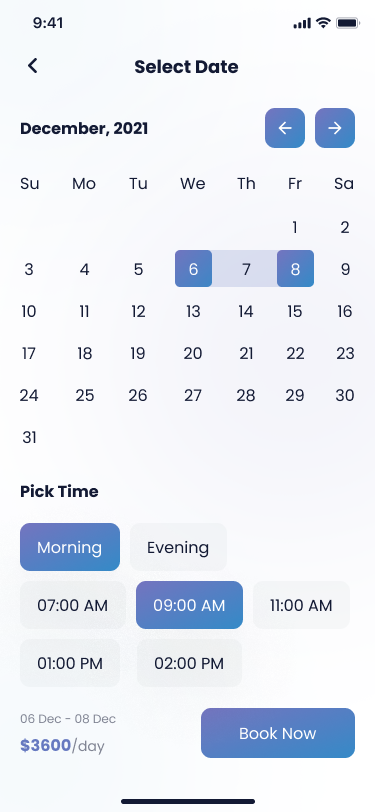
\includegraphics[width=\textwidth]{Images/Design/UIUX/renter/date.png}
        \caption{Chọn thời gian thuê}
    \end{subfigure}
    \hfill
    \begin{subfigure}[b]{0.32\textwidth}
        \centering
        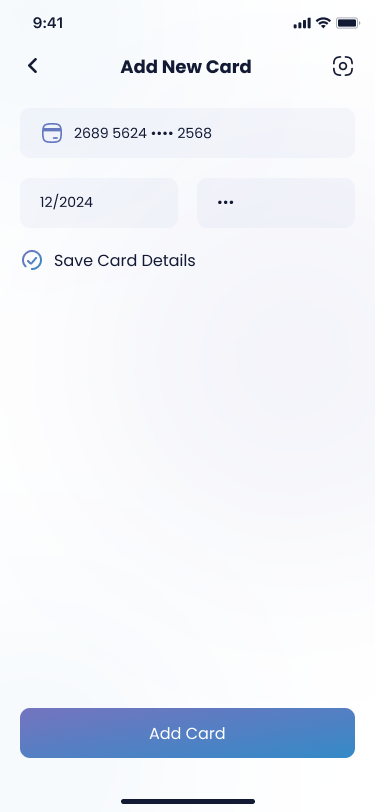
\includegraphics[width=\textwidth]{Images/Design/UIUX/renter/add-pay.png}
        \caption{Thêm ví thanh toán}
    \end{subfigure}
    \hfill
    \begin{subfigure}[b]{0.32\textwidth}
        \centering
        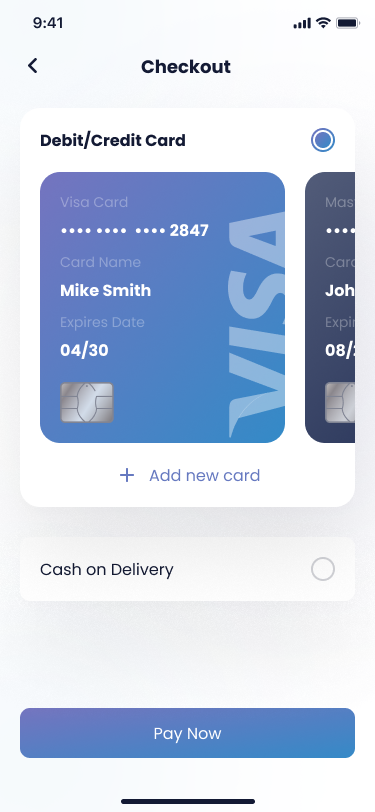
\includegraphics[width=\textwidth]{Images/Design/UIUX/renter/pay.png}
        \caption{Xác nhận \& Thanh toán}
    \end{subfigure}
    \caption{Quy trình đặt thuê xe (UC-04, UC-06)}
    \label{fig:ui-booking}
\end{figure}
Người dùng chọn thời gian thuê linh hoạt (tối thiểu 30 phút). Hệ thống AI gợi ý khung giờ “xanh” — khi xe ít được đặt và chủ xe đang online — giúp tăng tỷ lệ duyệt nhanh và giảm giá động. Màn hình thanh toán hiển thị rõ: phí thuê, phí nền tảng, tiền đặt cọc (hoàn lại 100\% nếu không hư hỏng), tổng tiền. Hỗ trợ nhiều phương thức: ví MoMo, ZaloPay, VNPay, thẻ tín dụng. Quy trình chỉ 3 bước, thời gian hoàn tất trung bình dưới 45 giây theo kết quả kiểm thử người dùng.
% \subsubsection*{4. Trong chuyến đi \& Trả xe}

% \begin{figure}[H]
%     \centering
%     \begin{subfigure}[b]{0.32\textwidth}
%         \centering
%         \includegraphics[width=\textwidth]{Images/UI/active_trip.png}
%         \caption{Theo dõi chuyến đi realtime}
%     \end{subfigure}
%     \hfill
%     \begin{subfigure}[b]{0.32\textwidth}
%         \centering
%         \includegraphics[width=\textwidth]{Images/UI/return_confirm.png}
%         \caption{Xác nhận trả xe}
%     \end{subfigure}
%     \hfill
%     \begin{subfigure}[b]{0.32\textwidth}
%         \centering
%         \includegraphics[width=\textwidth]{Images/UI/review.png}
%         \caption{Đánh giá sau chuyến}
%     \end{subfigure}
%     \caption{Theo dõi và kết thúc chuyến (UC-05, UC-07)}
%     \label{fig:ui-trip}
% \end{figure
\newpage
\subsubsection{Quản lý xe (dành cho chủ xe)}

\begin{figure}[H]
    \centering
    \begin{subfigure}[b]{0.32\textwidth}
        \centering
        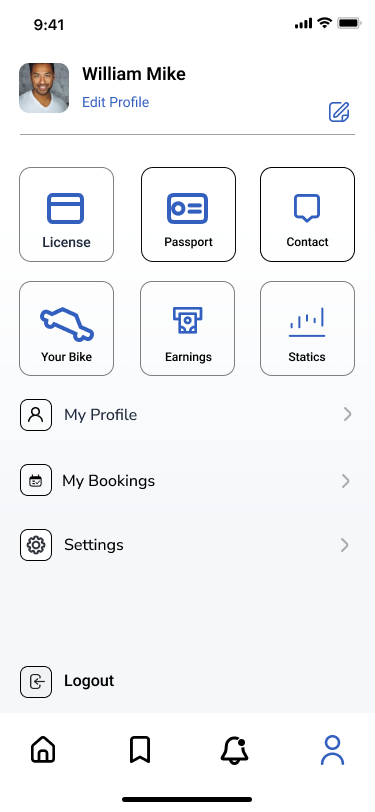
\includegraphics[width=\textwidth]{Images/Design/UIUX/owner/profile.png}
        \caption{Hồ sơ chủ xe}
    \end{subfigure}
    \hfill
    \begin{subfigure}[b]{0.32\textwidth}
        \centering
        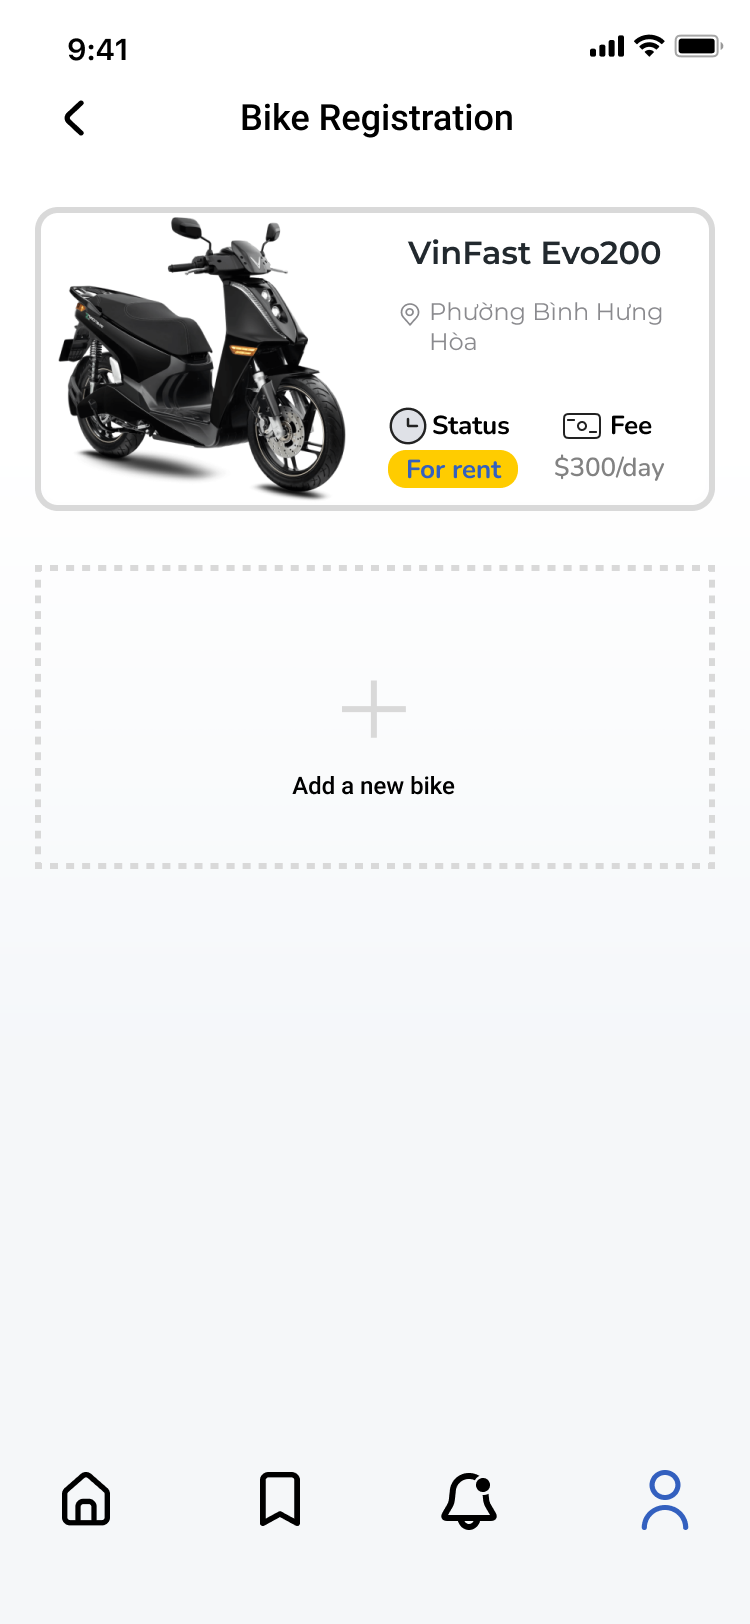
\includegraphics[width=\textwidth]{Images/Design/UIUX/owner/my-bike.png}
        \caption{Danh sách xe của tôi}
    \end{subfigure}
    \hfill
    \begin{subfigure}[b]{0.32\textwidth}
        \centering
        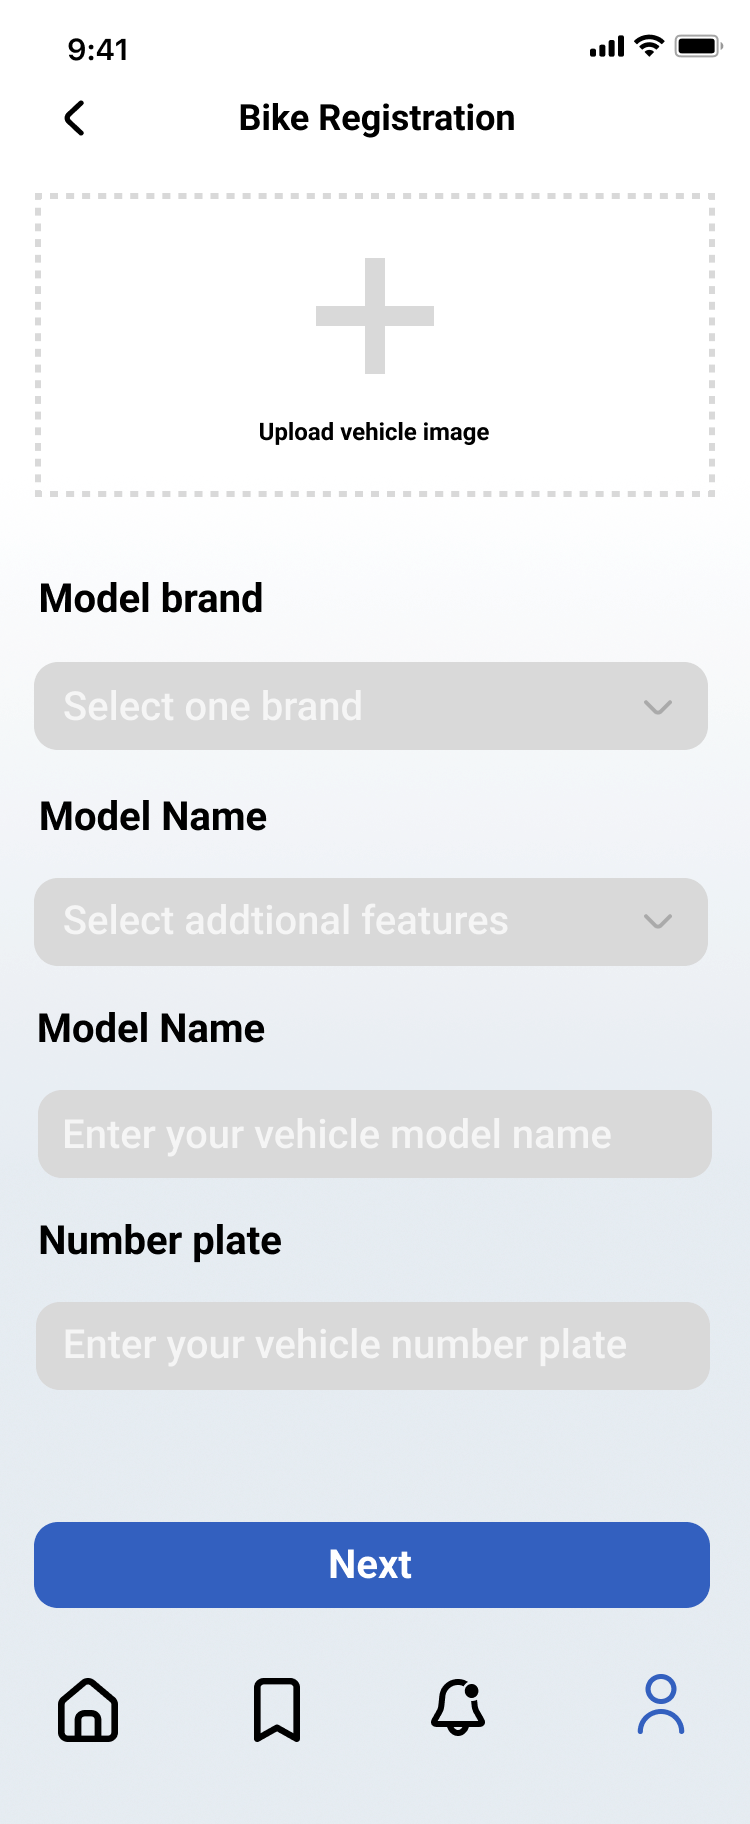
\includegraphics[width=\textwidth]{Images/Design/UIUX/owner/add.png}
        \caption{Đăng ký xe mới}
    \end{subfigure}
        \caption{Quản lý xe và thu nhập (UC-08, UC-09, UC-15)}

    \label{fig:ui-owner}
\end{figure}
Chủ xe có thể thêm xe mới chỉ trong 2 phút với các trường bắt buộc: biển số, hình ảnh 360°, giấy đăng ký xe. Màn hình danh sách xe hiển thị trạng thái realtime (khả dụng / đang thuê / bảo trì) và mức pin. Phần thu nhập thể hiện biểu đồ doanh thu theo ngày/tuần/tháng, tỷ lệ sử dụng xe giúp chủ xe tối ưu thời gian cho thuê.
% \subsubsection*{6. Dashboard quản trị viên (Web Admin – React.js)}

% \begin{figure}[H]
%     \centering
%     \begin{subfigure}[b]{0.45\textwidth}
%         \centering
%         \includegraphics[width=\textwidth]{Images/UI/admin_dashboard.png}
%         \caption{Tổng quan hệ thống}
%     \end{subfigure}
%     \hfill
%     \begin{subfigure}[b]{0.45\textwidth}
%         \centering
%         \includegraphics[width=\textwidth]{Images/UI/admin_vehicle_approval.png}
%         \caption{Duyệt xe chờ}
%     \end{subfigure}
%     \caption{Giao diện quản trị web}
%     \label{fig:ui-admin}
% \end{figure}

% Tất cả giao diện đều được thiết kế responsive, hỗ trợ chế độ tối (dark mode), tiết kiệm pin và dữ liệu di động theo yêu cầu phi chức năng đã nêu ở mục \ref{fig:non-functional}.

\newpage
\section{Triển khai}
\subsection{Tổng quan hệ thống}
\begin{figure}[H]
    \centering
    \includegraphics[width=1.0\textwidth]{Images/Arch/arch-w-tech.png}
    \caption{Sơ đồ triển khai hệ thống}
    \label{fig:implement-diagram}
\end{figure}
Hình \ref{fig:implement-diagram} trình bày sơ đồ triển khai hệ thống, thể hiện cách các thành phần được phân bố và tích hợp với công nghệ đã lựa chọn. 
% Kiến trúc Clean Architecture được áp dụng để đảm bảo tính tách biệt giữa các lớp: Entities (Domain Entities), Use Cases (Application Business Rules), Controllers/Presenters (Interface Adapters), và Frameworks/Drivers (Data Access, External Services). 

\subsubsection{Phía Client-side}
- Ứng dụng di động Flutter phục vụ cả hai vai trò chính: Renter và Owner. 
Người dùng kết nối qua WebSocket để nhận cập nhật realtime và qua HTTP để thực hiện các request thông thường.\\
- Giao diện quản trị Admin UI được triển khai riêng (có thể là web-based với React).

\subsubsection{Phía Server-side}
Hệ thống backend được xây dựng trên NestJS Application Server, tuân thủ nghiêm ngặt Clean Architecture với bốn lớp chính:\\
(1) \textbf{Domain}: Chứa Domain Entities – các thực thể nghiệp vụ cốt lõi (User, Vehicle, Booking, Payment, Review...).\\
(2) \textbf{Application Business Rules}: Bao gồm các Use Cases (AdminUseCase, RenterUseCase, OwnerUseCase) đại diện cho các quy tắc nghiệp vụ ứng dụng.\\
(3) \textbf{Interface Adapters}:\\
  - Controllers (AdminController, RenterController, OwnerController) xử lý HTTP requests từ API Gateway.\\
  - Presenters (AdminPresenter, RenterPresenter, OwnerPresenter) chuyển đổi dữ liệu từ Use Cases sang định dạng phù hợp để trả về client.\\
(4) \textbf{Frameworks \& Drivers}:\\
  - Data Access layer với InterfaceRepository và RepositoryImplementation sử dụng Prisma ORM để tương tác với PostgreSQL Database.\\
  - Redis Cache cho caching và hỗ trợ realtime.\\
  - External Services: PDF Export Service, MonitorService, GPS Service, File Upload Service, Map Service.

\subsubsection{Giao tiếp realtime và không đồng bộ}
- NestJS EventEmitter phát ra các Message (ví dụ: BookingEvent) đến Lightweight Event Bus\\
- WebSocket Gateway (Notify Module) xử lý kết nối realtime từ các Socket Client, nhận message là các Booking Event và xử lý tương ứng từ Booking Publisher.\\
- Mở rộng trong tương lại: AI Recommendation module (Python-based) được tích hợp qua Message Broker (RabbitMQ/Kafka), với các subscriber riêng cho 
File, Data Training và Updated Data. Publisher từ backend gửi dữ liệu đến Message Broker để AI xử lý.
\subsubsection{Lưu trữ và external integration}
- PostgreSQL là cơ sở dữ liệu chính, hỗ trợ đầy đủ transaction và relational data.\\
- Redis được sử dụng cho cache và pub/sub realtime.\\
- Các dịch vụ bên ngoài (GPS, Map, File Upload, Monitor, PDF Export) được gọi qua các adapter trong lớp Frameworks \& Drivers.
\subsection{MODULE 1: Authentication \& User Management}

\subsubsection{Mục tiêu}
Module Authentication đảm nhận việc xác thực người dùng và quản lý phiên làm việc trong toàn bộ hệ thống. Mục tiêu chính là tạo ra một cơ chế đăng nhập an toàn, hỗ trợ multi-role (RENTER, OWNER, ADMIN), và cho phép người dùng quản lý tài khoản của mình bao gồm cả việc nâng cấp vai trò.

\subsubsection{Công nghệ sử dụng}
Backend sử dụng NestJS với Passport JWT strategy để xác thực. Password được hash bằng bcrypt với salt rounds = 10. JWT token có thời gian sống 7 ngày, được verify tự động thông qua JwtAuthGuard. Email OTP được gửi qua NodeMailer với Gmail SMTP. Frontend Flutter lưu trữ token trong SharedPreferences và tự động attach vào mọi request thông qua Dio interceptor.

\subsubsection{Quy trình đăng ký người dùng}
Quy trình đăng ký bắt đầu khi người dùng điền form đăng ký trên mobile app. Hệ thống client thực hiện validation cơ bản (email format, phone format, password strength) trước khi gửi request đến backend.

Backend nhận request và thực hiện validation toàn diện hơn. Đầu tiên, hệ thống kiểm tra xem email đã tồn tại hay chưa bằng cách query database. Nếu email đã được sử dụng, trả về lỗi Conflict. Tương tự với số điện thoại - hệ thống đảm bảo mỗi số điện thoại chỉ được đăng ký một lần.

Khi validation thành công, password được hash sử dụng bcrypt. Hash được tính toán với 10 salt rounds để đảm bảo bảo mật. User record được tạo trong database với role mặc định là RENTER và status là ACTIVE. Trust score khởi tạo ở mức 100 điểm.

Sau khi tạo user thành công, hệ thống generate JWT token chứa userId, email và roles. Token này được trả về client cùng với thông tin user (không bao gồm password). Client lưu token vào local storage và sử dụng cho các request tiếp theo.

\subsubsection{Quy trình đăng nhập}
Người dùng nhập email và password vào form đăng nhập. Client gửi request đến endpoint \texttt{/auth/login} với credentials. Backend tìm user theo email trong database. Nếu không tìm thấy, trả về lỗi Unauthorized với message chung chung để tránh leak thông tin.

Khi tìm thấy user, hệ thống verify password bằng cách so sánh hash. Bcrypt tự động handle việc extract salt từ stored hash và compute hash của password input, sau đó so sánh. Nếu password không khớp, trả về lỗi tương tự như trường hợp không tìm thấy user.

Trước khi generate token, hệ thống kiểm tra user status. Nếu status là BLOCKED, từ chối đăng nhập và thông báo user liên hệ support. Nếu mọi thứ hợp lệ, JWT token được generate và trả về client.

Client nhận token và lưu vào storage. Từ thời điểm này, mọi request đến protected endpoints đều attach token vào Authorization header dưới dạng "Bearer \{token\}".

\subsubsection{Cơ chế xác thực JWT}
Mỗi khi client gửi request đến protected endpoint, NestJS JwtAuthGuard được trigger. Guard này extract token từ Authorization header, verify signature sử dụng JWT\_SECRET, và kiểm tra expiration time.

Nếu token hợp lệ, JwtStrategy được gọi. Strategy này decode payload để lấy userId, sau đó load user từ database. Hệ thống kiểm tra lại user status - nếu user đã bị block sau khi token được issue, request sẽ bị từ chối.

User object được attach vào request context thông qua CurrentUser decorator. Từ đây, controller có thể access user information một cách type-safe. Nếu ở bất kỳ bước nào token invalid hoặc user không hợp lệ, request bị reject với status 401 Unauthorized.

\subsubsection{Quy trình reset mật khẩu}
Người dùng quên mật khẩu và truy cập màn hình "Forgot Password", nhập email của mình. Client gửi request đến \texttt{/auth/forgot-password}. Backend verify email tồn tại trong database. Nếu không tồn tại, trả về lỗi 404 với message rõ ràng.

Hệ thống generate OTP code 5 chữ số random. OTP được lưu vào database với thông tin: code, userId, type (PASSWORD\_RESET), expiresAt (current time + 10 minutes), và isUsed flag (false). Trước khi tạo OTP mới, tất cả OTP cũ của user với type PASSWORD\_RESET được mark là isUsed = true để tránh tái sử dụng.

Email chứa OTP được gửi qua NodeMailer. Email template được format đẹp với branding và instruction rõ ràng. Trong development environment, nếu email service không được config, OTP được log ra console để developer test.

User nhận email, nhập OTP vào app. Client gửi OTP đến endpoint \texttt{/auth/verify-otp}. Backend tìm OTP record với điều kiện: userId khớp, code khớp, type là PASSWORD\_RESET, isUsed = false, và expiresAt > current time. Nếu không tìm thấy, trả về lỗi "Invalid or expired OTP".

Khi OTP valid, client cho phép user nhập mật khẩu mới. Request đến \texttt{/auth/reset-password} chứa email, OTP và new password. Backend thực hiện verify OTP lần nữa, hash password mới, update vào database, và mark OTP là isUsed. Transaction được sử dụng để đảm bảo cả hai operations (update password và mark OTP) đều thành công hoặc đều fail.

\subsubsection{Quy trình nâng cấp lên OWNER}
User với role RENTER muốn trở thành owner để đăng ký xe. User truy cập màn hình "Become Owner" trong app, điền form đăng ký xe đầu tiên (yêu cầu bắt buộc để trở thành owner). Form bao gồm thông tin xe: license plate, model, brand, giá thuê, ảnh xe, và giấy tờ xe.

Client gửi request đến \texttt{/auth/become-owner} với JWT token và vehicle data. Backend verify user đang đăng nhập, kiểm tra user chưa có role OWNER. Nếu đã là owner, trả về message thông báo không cần upgrade nữa.

Hệ thống thực hiện transaction: thêm role OWNER vào mảng roles của user, và tạo vehicle record với status PENDING\_APPROVAL. Cả hai operations phải thành công. Sau khi commit transaction, JWT token mới được generate với roles đã update (bây giờ bao gồm cả RENTER và OWNER).

Token mới được trả về client. Client update local storage với token mới này. User interface refresh để hiển thị các features dành cho owner như "My Vehicles", "Manage Bookings", etc.

\subsection{MODULE 2: Vehicle Management}

\subsubsection{Mục tiêu}
Vehicle Management module quản lý toàn bộ vòng đời của xe từ khi đăng ký, duyệt, cho thuê, bảo trì cho đến khi ngừng hoạt động. Module này phải đảm bảo chỉ owner được phép quản lý xe của mình, và admin có quyền kiểm soát toàn bộ xe trong hệ thống.

\subsubsection{Công nghệ sử dụng}
Backend sử dụng Prisma ORM để interact với PostgreSQL database. File uploads được xử lý bằng Multer middleware, lưu trữ tạm trong memory trước khi upload lên AWS S3 thông qua AWS SDK v3. Frontend sử dụng image\_picker package để chọn ảnh từ gallery hoặc camera, compress ảnh trước khi upload để tiết kiệm bandwidth.

\subsubsection{State machine của Vehicle}
Mỗi vehicle có một lifecycle rõ ràng được quản lý bởi state machine. State ban đầu khi owner đăng ký xe là PENDING\_APPROVAL. Ở state này, xe chưa visible cho renters, chỉ admin review và approve.

Admin có thể approve hoặc reject xe. Nếu approve, xe chuyển sang AVAILABLE và xuất hiện trong search results. Nếu reject, xe chuyển sang REJECTED với lý do từ chối được lưu lại. Owner có thể edit thông tin và submit lại để request approval.

Từ AVAILABLE, xe có thể chuyển sang nhiều states khác nhau. Khi có booking được confirm và trip bắt đầu, xe tự động chuyển sang RENTED. Owner không thể edit thông tin xe hoặc thay đổi availability khi đang RENTED.

Owner có thể chủ động chuyển xe từ AVAILABLE sang MAINTENANCE khi cần sửa chữa hoặc bảo trì. Ở state này, xe không xuất hiện trong search results. Sau khi bảo trì xong, owner chuyển lại AVAILABLE.

Admin có quyền lock vehicle bằng cách chuyển sang state LOCKED trong trường hợp vi phạm policy hoặc có dispute. State LOCKED cao hơn tất cả các states khác - owner không thể thay đổi gì cho đến khi admin unlock.

\subsubsection{Quy trình đăng ký xe mới}
Owner đã được upgrade role, truy cập màn hình "Register Vehicle". Form yêu cầu các thông tin bắt buộc: license plate (biển số xe theo format Việt Nam), model, brand, giá thuê theo giờ và theo ngày, địa chỉ đỗ xe, và ít nhất một ảnh xe.

Khi owner submit form, client thực hiện validation cơ bản. Với ảnh xe, client compress ảnh xuống dưới 1MB mỗi ảnh để tối ưu upload speed. Nếu có location permission, client tự động lấy GPS coordinates của owner để fill vào form.

Client gửi ảnh lên server trước thông qua endpoint \texttt{/upload/vehicle-images}. Request sử dụng multipart/form-data với max 10 files. Backend validate file types (chỉ chấp nhận jpg, png, webp, gif) và file size (max 5MB mỗi file).

Mỗi file được rename thành format \texttt{vehicles/\{uuid\}.\{extension\}} để tránh conflict. File được upload lên S3 bucket với public-read access. S3 trả về public URL cho mỗi ảnh. URLs này được collect lại và client sẽ submit trong vehicle registration payload.

Khi có đủ image URLs, client gửi request tạo xe đến \texttt{/vehicles}. Payload bao gồm tất cả thông tin xe và mảng image URLs. Backend verify user có role OWNER, kiểm tra license plate chưa tồn tại trong database (unique constraint).

Vehicle record được tạo với status PENDING\_APPROVAL và isAvailable = true. Owner được redirect đến "My Vehicles" page với message thông báo xe đang chờ duyệt. Notification được gửi cho admin về có xe mới cần review.

\subsubsection{Quy trình tìm kiếm xe}
Renter mở app, vào màn hình "Find Vehicle". Giao diện hiển thị search bar và filters. Client request location permission để lấy current location của renter. Nếu được cấp, location được sử dụng làm default search center.

Renter có thể filter theo: vehicle type (scooter, bike, motorcycle), brand, price range (min/max per hour), minimum rating, và distance radius (default 5km). Client build query parameters và gửi đến \texttt{/vehicles/available}.

Backend query database với điều kiện: status = AVAILABLE và isAvailable = true. Nếu có filters, thêm WHERE clauses tương ứng. Kết quả được sort theo distance từ search center (nếu có location) hoặc theo creation date mới nhất.

Pagination được implement với default limit = 20 items per page. Response bao gồm array vehicles, total count, và pagination metadata. Client hiển thị vehicles dưới dạng cards với ảnh đầu tiên, rating, price, và distance.

Renter tap vào một vehicle card để xem chi tiết. Client fetch full vehicle details từ \texttt{/vehicles/:id}. Response bao gồm đầy đủ vehicle info, owner info (name, avatar, trust score, response time), và array reviews. Owner password và sensitive info không được include trong response.

\subsubsection{Quy trình cập nhật thông tin xe}
Owner vào "My Vehicles", chọn một xe, tap "Edit". Form được pre-fill với thông tin hiện tại. Owner có thể thay đổi description, price, address, thêm hoặc xóa ảnh, và thay đổi availability status.

Một số fields không được phép edit: license plate (immutable), brand và model (nếu muốn đổi phải đăng ký xe mới). Owner cũng không thể tự thay đổi status thành RENTED hoặc LOCKED - chỉ có thể toggle giữa AVAILABLE và MAINTENANCE.

Khi submit, client gửi PATCH request đến \texttt{/vehicles/:id} với only changed fields (không gửi toàn bộ object). Backend verify ownership bằng cách check vehicle.ownerId === currentUser.id. Nếu không phải owner, trả về 403 Forbidden.

Backend validate status transition. Owner chỉ được phép: AVAILABLE $\rightarrow$ MAINTENANCE, MAINTENANCE $\rightarrow$ AVAILABLE. Mọi transition khác đều bị reject. Nếu xe đang RENTED, không được phép thay đổi status.

Update được apply vào database. Nếu có thay đổi về giá hoặc availability, hệ thống có thể emit event để notify users đang watch vehicle này. Response trả về updated vehicle object.

\subsubsection{Quy trình xóa xe}
Owner có thể xóa xe nếu xe không còn sử dụng hoặc đã bán. Trong "My Vehicles", owner tap menu và chọn "Delete". App hiển thị confirmation dialog warning rằng action này không thể undo.

Client gửi DELETE request đến \texttt{/vehicles/:id}. Backend verify ownership như thường lệ. Quan trọng nhất là check vehicle status - không được phép xóa xe đang RENTED. Nếu đang có active booking, trả về error message yêu cầu đợi booking kết thúc.

Hệ thống cũng check xem có booking nào trong tương lai không. Nếu có confirmed bookings sắp tới, cũng không cho phép xóa để tránh impact đến renters. Owner cần cancel hết bookings trước khi có thể delete xe.

Khi validation pass, vehicle record bị xóa khỏi database. Cascade delete được config trong database schema để tự động xóa related records như reviews và bookings đã hoàn thành. Ảnh trên S3 không bị xóa ngay mà được giữ lại cho audit log.

\subsection{MODULE 3: Booking System}

\subsubsection{Mục tiêu}
Booking System là trái tim của toàn bộ platform. Module này quản lý vòng đời booking từ khi renter tạo request, owner approve/reject, đến khi trip hoàn thành. Mục tiêu là tạo ra một flow trơn tru, rõ ràng, và an toàn cho cả hai bên tham gia giao dịch.

\subsubsection{Công nghệ sử dụng}
Backend sử dụng NestJS EventEmitter để implement event-driven architecture, tách biệt booking logic và notification logic. Database transactions được sử dụng ở mọi operation có nhiều bước để đảm bảo data consistency. Frontend implement optimistic updates để UI responsive ngay lập tức, sau đó sync với server state.

\subsubsection{State machine của Booking}
Booking lifecycle bắt đầu ở state PENDING khi renter tạo request. Từ PENDING, có ba possible transitions: CONFIRMED (owner approve), REJECTED (owner reject), hoặc CANCELLED (renter cancel hoặc booking timeout).

Từ CONFIRMED, booking chuyển sang ONGOING khi renter start trip ở pickup time. ONGOING là state active - vehicle đang được sử dụng. Từ ONGOING chỉ có một way forward: COMPLETED khi trip kết thúc thành công.

CANCELLED và COMPLETED là terminal states - không có transition nào từ đây. REJECTED cũng là terminal state, nhưng có một exception: admin có thể manually move từ REJECTED về PENDING nếu có dispute.

Mỗi state transition đều được log với timestamp và actor (ai thực hiện action). Audit trail này quan trọng cho dispute resolution và analytics.

\subsubsection{Quy trình tạo booking}
Renter đã chọn xe và time slot, tap "Book Now" ở vehicle detail page. Client mở booking form hiển thị summary: vehicle info, selected time range, calculated price (hourly hoặc daily rate), và deposit amount.

Form cho phép renter nhập optional notes cho owner (ví dụ: "Tôi cần xe để đi du lịch Đà Lạt"). Client validate time range: start time phải sau current time, end time phải sau start time, và duration phải reasonable (không quá 30 ngày).

Khi renter confirm, client gửi POST request đến \texttt{/bookings} với vehicleId, startTime, endTime, và notes. Backend bắt đầu một series validations quan trọng.

Đầu tiên, verify renter không phải là chủ xe. Nếu user.id === vehicle.ownerId, trả về error "You cannot book your own vehicle". Check này tránh circular booking và gaming system.

Tiếp theo, check vehicle availability. Vehicle phải có status = AVAILABLE và isAvailable = true. Nếu không, trả về error với current vehicle status để renter hiểu lý do.

Quan trọng nhất là check time conflicts. Backend query database tìm tất cả bookings của vehicle này với status là PENDING, CONFIRMED, hoặc ONGOING. Với mỗi existing booking, check xem có overlap với requested time range không.

Overlap detection sử dụng logic: (start1 < end2) AND (start2 < end1). Nếu condition này true, có conflict. Hệ thống trả về error "Vehicle already booked for this time slot" kèm với suggested alternative times.

Khi validations pass, system calculate total price. Nếu duration >= 24 hours, sử dụng daily rate. Nếu < 24 hours, sử dụng hourly rate. Total price = (rate $\times$ duration) rounded up. Deposit được lấy từ vehicle.deposit field.

Booking record được create với status = PENDING, calculated prices, và link đến user, owner, và vehicle. Ngay sau khi create, hệ thống emit event "booking.created" với booking details.

Response được trả về renter với booking object. Client show success message và navigate đến booking detail page. Renter thấy status PENDING với message "Waiting for owner approval".

\subsubsection{Quy trình owner approve booking}
Owner nhận real-time notification (thông qua WebSocket hoặc FCM) về có booking request mới. Notification payload chứa bookingId và basic info. Owner tap notification để mở booking detail page.

Page hiển thị đầy đủ thông tin: renter profile (name, avatar, trust score, số trips đã hoàn thành), vehicle info, requested time range, pricing breakdown, và renter's notes. Owner có context đầy đủ để quyết định.

Owner có hai buttons: "Approve" (green) và "Reject" (red). Nếu tap Approve, một confirmation dialog xuất hiện cho phép owner nhập optional message cho renter (ví dụ: "Welcome! Please arrive on time").

Khi confirm approve, client gửi PATCH request đến \texttt{/owner/bookings/:id/approve} với optional message. Backend verify ownership: booking.ownerId phải match currentUser.id. Nếu không match, trả về 403.

Backend check booking status = PENDING. Nếu booking đã bị cancel hoặc reject, trả về error "Booking is no longer available for approval". Race condition này có thể xảy ra nếu renter cancel cùng lúc owner approve.

Hệ thống re-validate time conflicts một lần nữa. Trong khoảng thời gian từ khi booking được tạo đến khi owner approve, có thể có booking khác đã được approve cho cùng time slot (nếu owner approve nhiều bookings cùng lúc). Check này đảm bảo không có double booking.

Nếu validation pass, transaction bắt đầu: update booking status từ PENDING sang CONFIRMED, set confirmedAt timestamp, và save owner's message. Transaction commit, event "booking.approved" được emit với booking details.

Response trả về owner với updated booking object. Client update UI ngay lập tức để reflect confirmed status. Owner thấy booking move từ "Pending" sang "Confirmed" tab.

\subsubsection{Quy trình owner reject booking}
Owner review booking và quyết định reject. Có thể vì: time không convenient, renter trust score quá thấp, hoặc đơn giản là owner không muốn cho thuê nữa. Owner tap "Reject" button.

Dialog xuất hiện yêu cầu nhập lý do reject (required field). Lý do này sẽ được gửi cho renter để họ hiểu tại sao. Common reasons: "Vehicle not available at that time", "Need vehicle for personal use", "Renter profile concerns".

Client gửi PATCH request đến \texttt{/owner/bookings/:id/reject} với reason text. Backend verify ownership và status = PENDING như flow approve. Transaction update booking status sang REJECTED, set cancellationReason, và cancelledAt timestamp.

Event "booking.rejected" được emit. Response trả về owner. Client update UI và show success message "Booking rejected". Booking move sang "History" tab với REJECTED badge.

\subsubsection{Quy trình renter cancel booking}
Renter có thể cancel booking ở status PENDING hoặc CONFIRMED (trước khi trip start). Trong booking detail page, renter thấy "Cancel Booking" button. Tap button mở confirmation dialog warning về cancellation.

Dialog yêu cầu nhập cancellation reason. Client gửi PATCH request đến \texttt{/bookings/:id/cancel} với reason. Backend verify booking.renterId === currentUser.id và status cho phép cancel (PENDING hoặc CONFIRMED).

Transaction update status sang CANCELLED với cancellation metadata. Event "booking.cancelled" được emit với info về ai cancel (renter) và reason. Notification được gửi cho owner thông báo renter đã cancel.

Nếu booking ở gần pickup time (ví dụ: < 2 hours), system có thể apply cancellation penalty hoặc mark flag trên renter profile để track cancellation behavior. Policy này được define ở business level.

\subsubsection{Auto-expiry của pending bookings}
Backend chạy scheduled job (cron) mỗi 15 phút để scan pending bookings. Nếu booking đã pending quá X hours (ví dụ: 24 hours) mà chưa được approve, tự động cancel.

Job query bookings với status = PENDING và createdAt < (now - 24 hours). Với mỗi booking, update status sang CANCELLED với reason "Expired - no response from owner". Event được emit để notify renter.

Auto-expiry đảm bảo renters không phải đợi vô thời hạn và có thể book xe khác. Nó cũng giúp keep booking list của owners clean.

\subsection{MODULE 4: Notification System}

\subsubsection{Mục tiêu}
Notification System đảm bảo users luôn được thông báo kịp thời về mọi sự kiện quan trọng. Mục tiêu là delivery notification trong vòng < 1 second khi user online, và đảm bảo không miss notification khi offline thông qua FCM push.

\subsubsection{Công nghệ sử dụng}
Backend sử dụng Socket.IO cho WebSocket connections, NestJS EventEmitter cho event bus, Firebase Admin SDK cho push notifications. Frontend Flutter sử dụng socket\_io\_client cho WebSocket, firebase\_messaging cho FCM, và local notifications plugin cho in-app toasts.

\subsubsection{Kiến trúc Hybrid}
Notification system được thiết kế theo mô hình hybrid với ba channels: Database storage, WebSocket real-time, và FCM push. Ba channels này work together để đảm bảo zero message loss và optimal delivery time.

Database channel lưu trữ mọi notifications như permanent records. Mỗi notification có: id, receiverId, senderId, type, title, message, bookingId (optional), isRead flag, createdAt, và readAt timestamps. Database serve như source of truth và inbox history.

WebSocket channel deliver notifications real-time cho users đang online. Khi notification được tạo, system check nếu receiver đang có active WebSocket connection. Nếu có, notification được emit immediately đến client. Client hiển thị toast và update badge count.

FCM channel đảm bảo delivery cho offline users. Mọi notification đều được gửi qua FCM bất kể user online hay offline. FCM xử lý việc queue messages và deliver khi device online trở lại. System track FCM tokens trong database và handle token refresh automatically.

\subsubsection{Event-driven notification flow}
Notification flow bắt đầu từ business events. Khi có sự kiện xảy ra trong system (booking created, trip started, payment completed), service emit event thông qua EventEmitter. Event payload chứa đầy đủ context: actor, target, action, và related entities.

Event listeners được register ở notification module. Mỗi listener handle một loại event cụ thể. Ví dụ: BookingEventListener handle tất cả booking-related events như booking.created, booking.approved, booking.rejected, booking.cancelled.

Khi listener receive event, nó extract thông tin cần thiết, determine recipients (ai nên nhận notification), và compose notification content. Content được customize dựa trên recipient role và event type. Ví dụ: khi booking created, owner nhận "New booking request", còn admin nhận "New booking requires review".

Notification record được create trong database với all metadata. Ngay sau đó, system check xem recipient có đang online không bằng cách lookup trong WebSocket connection map. Nếu online, notification được emit qua WebSocket. Parallel với đó, FCM notification được trigger.

Flow này đảm bảo: notifications được persist (không mất), delivery nhanh nếu possible (WebSocket), và fallback robust nếu user offline (FCM). Architect tách biệt business logic và notification logic, make system dễ extend và maintain.

\subsubsection{WebSocket connection management}
Khi Flutter app start, SocketService được initialize trong main(). Service extract JWT token từ local storage và establish WebSocket connection đến server với token trong handshake auth.

Server-side NotificationGateway receive connection request. Gateway extract token từ handshake, verify token bằng JwtService. Nếu token invalid, connection bị reject immediately. Nếu valid, userId được extract từ token payload.

Gateway maintain một Map<userId, Set<socketId>> để track connections. Một user có thể có nhiều active connections nếu login từ nhiều devices. Khi connection established, socketId được add vào Set của user đó.

Client socket được join vào personal room với name format \texttt{user\_\$\{userId\}}. Room concept trong Socket.IO cho phép broadcast message đến tất cả sockets trong room. Khi cần send notification đến user, server emit đến room này, và tất cả devices của user receive message.

Server gửi confirmation message "connected" với userId về client. Client setup event listeners cho các notification types: booking\_request, booking\_confirmed, booking\_rejected, booking\_cancelled, trip\_started, trip\_completed, payment\_success.

Connection monitoring được implement. Nếu connection drop, client tự động reconnect với exponential backoff. Server track connection state và clean up Map khi socket disconnect.

\subsubsection{Notification delivery flow}
Khi notification được tạo, NotificationService execute delivery flow parallel. Flow bắt đầu bằng save notification to database. Database insert return generated id và timestamps.

Parallel task 1: Check user online status bằng NotificationGateway.isUserOnline(userId). Method này check xem userId có trong connection Map không. 
Nếu online, call gateway.sendToUser(userId, eventType, payload). Gateway emit message đến room \texttt{user\_\$\{userId\}}. 
All active sockets của user receive message instantly.

Parallel task 2: Query FCM tokens của user từ database. User có thể có nhiều tokens từ nhiều devices. 
Filter tokens với isActive = true. Compose FCM message với notification (title, body) và data payload (bookingId, type, etc).

FCM message được send qua Firebase Admin SDK. Method sendEachForMulticast() send đến multiple tokens cùng lúc và return results. 
Results indicate success/failure cho mỗi token. Failed tokens được check: nếu error code là invalid-token hoặc registration-token-not-registered, mark token as inactive trong database.

Client-side, WebSocket message được receive bởi SocketService. Service emit message vào notificationStream. 
NotificationListenerWidget listen stream này, trigger NotificationBloc reload, show toast notification, và play sound (optional).

FCM message được receive bởi FirebaseMessaging. Nếu app foreground, onMessage handler được trigger. Nếu background, onBackgroundMessage handler được trigger. 
Payload được parse và local notification được show với action buttons.

\subsubsection{Badge count management}
Badge count represent số lượng unread notifications. Count này được display trên notification icon trong app bar. 
Count phải update real-time khi có notification mới hoặc khi user đọc notifications.

Initial load: Khi app start, client gửi GET \texttt{/notifications/unread-count}. Server query database với condition \texttt{receiverId = userId AND isRead = false}, return count. 
Client lưu count vào NotificationBloc state.

Real-time update: Khi notification mới arrive qua WebSocket, NotificationListenerWidget trigger NotificationBloc reload. 
Bloc gọi repository fetch notifications, trong đó có unreadCount. New state được emit với updated count. Badge widget rebuild và animate count increase.

Mark as read: Khi user tap notification item để view detail, hoặc tap "Mark all as read", client gửi PATCH \texttt{/notifications/read} hoặc \texttt{/notifications/read-all}. 
Server update isRead = true và set readAt timestamp. Response confirm success. Client trigger bloc reload để fetch updated count.

Badge animation: Khi count increase, badge widget thực hiện scale animation để draw attention. Animation được control bởi AnimationController với duration 300ms và curve elasticOut.

% \subsection{MODULE 5: Trip Management}

% \subsubsection{Mục tiêu}
% Trip Management module quản lý physical usage của vehicle từ lúc renter nhận xe đến lúc trả xe. Module capture essential metrics: location, distance, battery usage, duration, và issues encountered. Data này serve multiple purposes: billing verification, dispute resolution, và vehicle maintenance scheduling.

% \subsubsection{Công nghệ sử dụng}
% Backend implement Haversine formula để calculate distance giữa start và end coordinates. Flutter sử dụng geolocator package để get GPS location và location permission. Location tracking có thể được enhance sau này với background tracking cho live trip monitoring.

% \subsubsection{Quy trình start trip}
% Booking đã được confirmed, pickup time đến. Renter mở app, vào booking detail page. Page hiển thị pickup location và "Start Trip" button. Button chỉ enabled khi current time trong khoảng [startTime - 15 minutes, startTime + 2 hours] để allow flexibility.

% Renter tap "Start Trip". App request location permission nếu chưa có. Nếu user deny, show educational message explain why location needed và retry request. Nếu có permission, app get current location với desired accuracy = high.

% Form hiển thị với pre-filled data: current location (latitude, longitude, address reverse-geocoded from coordinates), và input field cho battery level. User được instruct đọc battery level từ vehicle dashboard và nhập vào form.

% Optional: User có thể chụp ảnh vehicle từ nhiều góc độ để document initial condition. Photos serve như evidence nếu có dispute về damages. Photos được upload tương tự như vehicle registration flow.

% Khi user confirm, client gửi POST request đến \texttt{/trips/start} với bookingId, start coordinates, start battery level, và optional photo URLs. Backend validate booking thuộc về user, booking status = CONFIRMED, và current time reasonable so với booking startTime.

% Trip record được create với status = ONGOING, start location, start battery, start timestamp. Transaction update booking status từ CONFIRMED sang ONGOING. Vehicle status update sang RENTED. Event "trip.started" được emit.

% Owner nhận notification "Renter has started the trip" với link đến trip tracking page. Renter được navigate đến active trip screen showing trip timer, current battery (estimate), và button "End Trip".

% \subsubsection{Trip monitoring}
% Trong suốt trip, renter có trip screen open hoặc minimized. Screen display:
% \begin{itemize}
% \item Elapsed time (counted từ startedAt)
% \item Estimated distance (nếu có background tracking)
% \item Current battery level (estimate dựa trên initial và time elapsed)
% \item Button "Report Issue" để report problems
% \end{itemize}

% Renter có thể report issues bất cứ lúc nào. Issues có thể là: vehicle malfunction, accident, flat tire, battery depleted unexpectedly. Reporting issue không cancel trip nhưng create record trong database.

% Issue report form có: severity (Low/Medium/High), description (text), và optional photos. Report được submit qua PATCH \texttt{/trips/:id/report-issue}. Backend save issue info và send notification cho owner immediately.

% Owner có thể contact renter để resolve issue. Trong serious cases, owner hoặc renter có thể decide end trip early. System support này thông qua admin intervention nếu cần.

% \subsubsection{Quy trình end trip}
% Khi renter trả xe, tap "End Trip" button. Form tương tự như start trip nhưng capture end state: end location, end battery level, issue report (nếu có). User được remind check vehicle condition và report mọi damages discovered.

% Client submit POST request đến \texttt{/trips/:id/end} với end data. Backend validate trip status = ONGOING và time elapsed reasonable (không thể end trip sau 2 phút start - likely error).

% Backend calculate trip metrics:
% \begin{itemize}
% \item Distance: Haversine formula between start và end coordinates, return khoảng cách theo km
% \item Duration: (endedAt - startedAt) converted to hours and minutes
% \item Battery used: (startBattery - endBattery) as percentage
% \end{itemize}

% Transaction update trip status sang COMPLETED, save end data và calculated metrics. Booking status update sang COMPLETED. Vehicle status update lại AVAILABLE. Vehicle.totalTrips increment by 1.

% Event "trip.completed" được emit. Notification được gửi cho cả owner và renter với trip summary. Renter được navigate đến trip summary page hiển thị all metrics và prompt rate vehicle.

% Owner receive notification và có thể review trip details. Nếu có issues reported, owner follow up với renter. Deposit được return hoặc deduct based trên vehicle condition.

% \subsubsection{Distance calculation}
% Haversine formula được dùng để calculate great-circle distance giữa hai points trên sphere. Formula account cho Earth's curvature, accurate cho distances up to $\sim$500km (sufficient cho motorbike trips).

% Formula steps:
% \begin{enumerate}
% \item Convert latitudes và longitudes từ degrees sang radians
% \item Calculate differences: dLat = lat2 - lat1, dLon = lon2 - lon1
% \item Calculate a = $\sin^2$(dLat/2) + $\cos$(lat1) $\times$ $\cos$(lat2) $\times$ $\sin^2$(dLon/2)
% \item Calculate c = 2 $\times$ atan2($\sqrt{a}$, $\sqrt{1-a}$)
% \item Distance = Earth radius (6371 km) $\times$ c
% \end{enumerate}

% Implementation trong backend service được test với known distances để ensure accuracy. Distance được round đến 1 decimal place (0.1 km) cho display purposes.

% \subsection{MODULE 6: Payment System}

% \subsubsection{Mục tiêu}
% Payment module handle financial transactions giữa renter và owner, với platform collecting fee. Mục tiêu là tạo flow payment đơn giản, secure, và support multiple payment methods popular ở Vietnam (VNPay, MoMo, Credit Card).

% \subsubsection{Công nghệ sử dụng}
% Backend integrate với payment gateways thông qua REST APIs. Each gateway có SDK riêng và webhook endpoint để receive callbacks. Payments được record trong database với full audit trail. Future enhancements có thể add escrow service để hold funds until trip completion.

% \subsubsection{Fee structure}
% Platform áp dụng fee structure: Renter pay total amount (rental cost + deposit). Platform take 15\% commission từ rental cost. Owner receive 85\% rental cost + full deposit back (assuming no damages).

% Example calculation:
% \begin{itemize}
% \item Rental: 200,000 VND (8 hours $\times$ 25,000/hour)
% \item Deposit: 300,000 VND
% \item Total renter pays: 500,000 VND
% \item Platform fee: 200,000 $\times$ 0.15 = 30,000 VND
% \item Owner receives: 170,000 + 300,000 = 470,000 VND
% \end{itemize}

% Fee được calculate tại booking creation time nhưng actual payment xảy ra khi trip confirmed hoặc completed (depending on business policy).

% \subsubsection{Quy trình payment}
% Booking confirmed, renter được prompt create payment. Flow có thể trigger immediately sau approval hoặc khi renter decide pay (before trip start). Trong booking detail page, "Proceed to Payment" button được enable.

% Renter tap button, được navigate đến payment method selection page. Page hiển thị available methods: VNPay, MoMo, Credit Card, Cash (cash chỉ available trong certain cases). Renter chọn preferred method.

% Client gửi POST request đến \texttt{/payments} với bookingId và selected method. Backend validate booking status appropriate cho payment và chưa có payment record. Payment record được create với status = PENDING, amount, platform fee, owner amount, method, và timestamps.

% Backend call payment gateway API để initiate payment session. Gateway return payment URL hoặc QR code. Client handle redirection hoặc display based on method:
% \begin{itemize}
% \item VNPay/MoMo: Redirect to gateway website trong webview
% \item Credit Card: Display card input form (PCI-compliant)
% \item QR Code: Display code cho user scan với banking app
% \end{itemize}

% User complete payment trên gateway. Gateway process transaction và redirect back to app với transaction result. Callback URL được hit với transaction status và verification signature.

% Backend verify callback authenticity bằng signature check. Nếu valid và transaction successful, update payment status từ PENDING sang COMPLETED, set transactionId và paidAt timestamp. Event "payment.success" được emit.

% Notifications được gửi cho both parties. Renter see success screen với receipt. Owner receive notification "Payment received" với payout details. Payment record được use cho generating invoices và financial reports.

% \subsubsection{Failure handling}
% Payment có thể fail vì nhiều reasons: insufficient funds, card declined, network timeout, user cancel. Mỗi failure có treatment khác nhau.

% Nếu payment failed, gateway callback indicate error với code. Backend update payment status sang FAILED, save error details trong gatewayResponse field. Renter được notified với user-friendly error message và option retry payment.

% User có thể retry payment multiple times. Each retry create new payment record linked to same booking. Previous failed payments kept cho audit but marked inactive. User được instruct fix issue (add funds, use different card) và try again.

% Nếu payment không completed before trip start time, booking có thể bị auto-cancel (business policy). Renter được notified trước khi cancel để có chance complete payment.

% Refunds được handle qua admin panel. Nếu trip cancelled sau payment, refund được initiate thông qua gateway refund API. Refund status được track separately và notification sent khi refund completed.

% \subsection{MODULE 7: Review System}

% \subsubsection{Mục tiêu}
% Review system cho phép renters rate và review vehicles sau khi complete trips. Reviews help future renters make informed decisions và incentivize owners maintain vehicles properly. System cũng track owner's response time và reliability.

% \subsubsection{Công nghệ sử dụng}
% Reviews được store trong relational database với foreign keys đến users và vehicles. Rating aggregation được calculate bằng simple average nhưng có thể enhance với weighted average dựa trên recency. Review moderation có thể được add sau này để filter spam hoặc inappropriate content.

% \subsubsection{Quy trình tạo review}
% Trip completed, renter được prompted rate vehicle. Prompt có thể show ngay trong trip completion screen hoặc via notification sau vài hours. Renter tap "Rate this vehicle" để mở review form.

% Form gồm hai parts:
% \begin{itemize}
% \item Rating: 1-5 stars với mô tả cho mỗi level (1 = Very Poor, 5 = Excellent)
% \item Comment: Text field cho detailed feedback (optional nhưng encouraged)
% \end{itemize}

% Renter submit review. Client gửi POST request đến \texttt{/reviews} với vehicleId, rating, và comment. Backend validate:
% \begin{itemize}
% \item User đã complete ít nhất một trip với vehicle này (query trips table)
% \item User chưa review vehicle này trước đó (one review per user per vehicle)
% \end{itemize}

% Nếu validations pass, review record được create. Immediately sau đó, system trigger recalculation của vehicle's average rating. Query tất cả reviews của vehicle, calculate average rating và count total reviews. Update vehicle.totalRating và vehicle.reviewCount.

% Owner được notified về có review mới. Review được display trên vehicle detail page cho tất cả users. Reviews được sort theo newest first, với option sort by highest/lowest rating.

% \subsubsection{Review display và filtering}
% Vehicle detail page có dedicated "Reviews" section. Section hiển thị:
% \begin{itemize}
% \item Overall rating (average với 1 decimal place, ví dụ: 4.7)
% \item Total review count
% \item Rating distribution (số lượng reviews cho mỗi star level)
% \item Individual reviews (paginated)
% \end{itemize}

% Mỗi review card show: reviewer name (hoặc anonymous), avatar, rating stars, comment text, và time ago. Owner có thể respond to reviews (future feature) để address concerns hoặc thank positive feedback.

% Users có thể filter reviews by rating (show only 5-star, 4-star, etc.) hoặc sort by newest/oldest. Search functionality có thể được add để find reviews mention specific keywords (ví dụ: "battery", "comfortable").

% Review system contribute đến trust building trong platform. High-rated vehicles get more bookings. Low-rated vehicles được flagged cho owner attention. Aggregate statistics được use trong search ranking algorithm.

\newpage
\section{Kế hoạch dự kiến cho giai đoạn 2 - Đồ Án Tốt Nghiệp}

Giai đoạn 2 (thời gian dự kiến từ tháng 1/2026 đến tháng 6/2026) nhóm sẽ tập trung hoàn thiện hệ thống, kiểm thử và triển khai. Lịch trình chi tiết được minh họa qua biểu đồ Gantt (Hình \ref{fig:gantt-chart}), với các giai đoạn chính:

\begin{itemize}
    \item \textbf{Tháng 1-2:} Refactor code theo Clean Architecture; hoàn thiện frontend cho quản lý chuyến đi, thanh toán và đánh giá (UC-02 đến UC-07, UC-13).
    \item \textbf{Tháng 2-3:} Tích hợp bản đồ Google Maps/API; xây dựng dashboard admin và hỗ trợ đa nền tảng iOS/Android (UC-10 đến UC-12).
    \item \textbf{Tháng 3-4:} Thực hiện kiểm thử đơn vị, tích hợp và end-to-end; kiểm toán bảo mật.
    \item \textbf{Tháng 4-5:} Triển khai backend/frontend; cập nhật tài liệu và báo cáo với chương triển khai, ảnh chụp màn hình.
    \item \textbf{Tháng 5-6:} Thu thập phản hồi demo, điều chỉnh; đo lường metrics và hoàn tất báo cáo cuối cùng.
\end{itemize}

Tổng thời gian: 6 tháng, với trọng tâm đảm bảo hệ thống ổn định (uptime >99.9\%) và trải nghiệm người dùng tối ưu.

\begin{figure}[H]
    \centering
    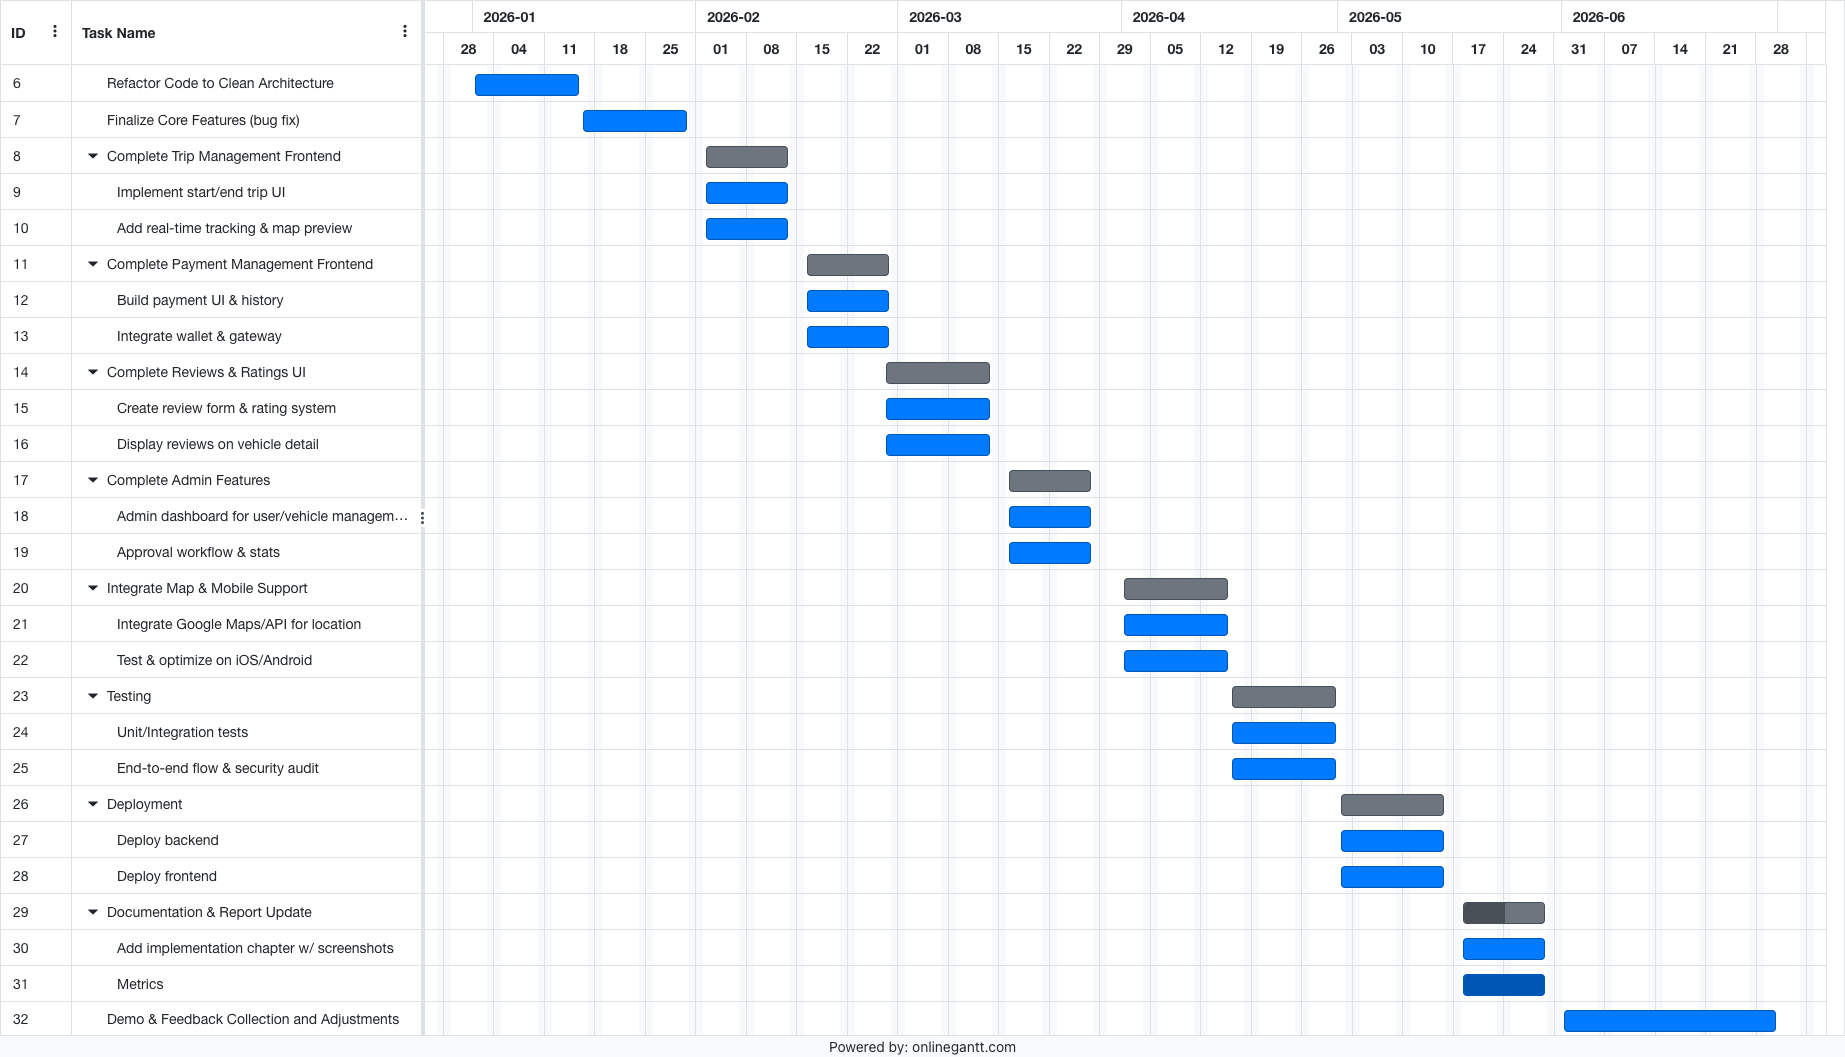
\includegraphics[width=1\textwidth]{Images/gantt-chart.png}
    \caption{Biểu đồ Gantt kế hoạch đồ án kỳ sau}
    \label{fig:gantt-chart}
\end{figure}

% \newpage
% \section{System Evaluation}

% \newpage
% \section{Conclusion}
% \subsection{Achievements}

% \subsection{Limitations}
% \subsection{Further improvements}

% \newpage
% % % \section{Tài liệu tham khảo}
% \sloppy
% \begin{thebibliography}{99}

% \bibitem{flipkartCCC2025}
% Flipkart Commerce Cloud, 
% \textit{``The Ultimate Guide to Building a Peer-to-Peer Marketplace,''} 
% Flipkart Commerce Cloud, 2025. 
% Available: \url{https://www.flipkartcommercecloud.com/guide-to-building-a-peer-to-peer-marketplace/}. 
% (Truy cập ngày 10/10/2025)

% \bibitem{dantri2023}
% Dân trí, 
% \textit{``Việt Nam có tỷ lệ người sử dụng xe máy cao nhất khu vực Đông Nam Á,''} 
% 14 Tháng 12, 2023. 
% Available: \url{https://dantri.com.vn/o-to-xe-may/viet-nam-co-ty-le-nguoi-su-dung-xe-may-cao-nhat-khu-vuc-dong-nam-a-20231214114542532.htm}

% \bibitem{kevesko2023}
% Kevesko, 
% \textit{``Việt Nam 'phá đảo' tỷ lệ người dùng xe máy tại Đông Nam Á,''} 
% 20 Tháng 12, 2023. 
% Available: \url{https://kevesko.vn/20231220/viet-nam-pha-dao-ty-le-nguoi-dung-xe-may--tai-dong-nam-a-27203888.html}

% \bibitem{phs2023}
% PHS, 
% \textit{``Chính sách xe điện ở Việt Nam đã đủ thúc đẩy người dân chuyển đổi,''} 
% 2023. 
% Available: \url{https://www.phs.vn/tin-tuc/chinh-sach-xe-dien-o-viet-nam-da-du-thuc-day-nguoi-dan-chuyen-doi/6250648}

% \bibitem{vnbusiness2023}
% VnBusiness, 
% \textit{``Xuất hiện cú hích, thị trường xe máy điện vẫn thiếu hai yếu tố quan trọng,''} 
% 2023. 
% Available: \url{https://vnbusiness.vn/thi-truong/xuat-hien-cu-hich-thi-truong-xe-may-dien-van-thieu-hai-yeu-to-quan-trong-1108286.html}

% \bibitem{chen2022}
% Y.~Chen, X.~Li, and M.~Qiu, 
% \textit{``Buying to share: How prosumption promotes purchases in peer-to-peer asset sharing,''} 
% ResearchGate, 2022. 
% Available: \url{https://www.researchgate.net/publication/358322592_Buying_to_share_How_prosumption_promotes_purchases_in_peer-to-peer_asset_sharing}

% \bibitem{ert2016}
% O.~Ert, A.~Fleischer, and N.~Magen, 
% \textit{``Trust in the Sharing Economy,''} 
% ResearchGate, 2016. 
% Available: \url{https://www.researchgate.net/publication/299812647_Trust_in_the_Sharing_Economy}

% \end{thebibliography}


\newpage
\printbibliography

\newpage
\section*{Phụ lục}
\addcontentsline{toc}{section}{Phụ lục}

Phần phụ lục này cung cấp liên kết đến các tài liệu hỗ trợ cho báo cáo, bao gồm chính sách pháp lý, khảo sát nhu cầu người dùng và các tài liệu thiết kế bổ sung.

\subsection*{A. Tài liệu pháp lý liên quan}
\addcontentsline{toc}{subsection}{A. Tài liệu pháp lý liên quan}

Các quy định pháp lý được sử dụng làm cơ sở để đánh giá tính hợp lệ của mô hình cho thuê xe máy điện, giao dịch điện tử và xử lý dữ liệu cá nhân:

\url{https://drive.google.com/file/d/17tyYIoYQgS55XRo3lMkTFauNXceZZbh2/view?usp=drive_link}

\vspace{10pt}

\subsection*{B. Kết quả khảo sát nhu cầu cộng đồng}
\addcontentsline{toc}{subsection}{B. Kết quả khảo sát nhu cầu cộng đồng}

Khảo sát được thực hiện để đánh giá mức độ quan tâm đối với mô hình thuê xe máy điện theo giờ, các tính năng người dùng mong muốn và thói quen sử dụng phương tiện di chuyển.

\begin{itemize}
    \item Form khảo sát (Google Form):
    
    \url{https://docs.google.com/forms/d/e/1FAIpQLScdU2fNqEeZQIFWnPs1rlXdPqpPLl07l_Q1lZIT_emHEnrG8g/viewform?usp=dialog}

    \item Bảng tổng hợp kết quả khảo sát (Google Sheets):  
    
    \url{https://drive.google.com/file/d/1qalHs-whOtyt8GSPV6-ShBEndhdr-MAg/view?usp=sharing}
\end{itemize}

\vspace{10pt}

\subsection*{C. Tài liệu thiết kế bổ sung}
\addcontentsline{toc}{subsection}{C. Tài liệu thiết kế bổ sung}

Bao gồm các tài liệu không đưa đầy đủ vào phần nội dung chính của báo cáo.

\begin{itemize}
    \item Prototype giao diện trên Figma:  
    
    \url{https://www.figma.com/proto/PM7XgY1isY4DmazIL1I40o/P2P-Electric-Scooter-Sharing-App?node-id=0-1&t=xyMUibPTbahANB60-1}

    % \item Sơ đồ ERD phiên bản đầy đủ:  
    % \url{https://drive.google.com/your-erd-link}

    % \item Tài liệu API (OpenAPI/Swagger):  
    % \url{https://your-api-docs-link}
\end{itemize}

\vspace{10pt}

\subsection*{D. Mã nguồn hệ thống}
\addcontentsline{toc}{subsection}{D. Mã nguồn hệ thống}

Toàn bộ mã nguồn của hệ thống được quản lý tập trung trong một tổ chức GitHub, bao gồm mã nguồn phía máy chủ (backend), ứng dụng người dùng (mobile app) và giao diện quản trị (admin web).  
Mã nguồn được công bố nhằm phục vụ mục đích tham khảo, đánh giá kỹ thuật và phát triển mở rộng trong tương lai.

\url{https://github.com/DACN-P2P-Electric-Motorbike}


\end{document}
